\documentclass[a4paper, 12pt, openany, twoside]{book} %oneside

\usepackage[utf8]{inputenc}
\usepackage[russian]{babel}
\usepackage{setspace}
\usepackage[left=30mm, top=20mm, right=15mm, bottom=20mm, nohead, footskip=10mm]{geometry} % настройки полей документа
\usepackage{lscape}
\usepackage{graphicx}
\usepackage{graphics}
\usepackage{subfigure}
\usepackage{indentfirst}
\usepackage[margin=10pt,font=small,labelfont=bf, labelsep=endash]{caption}
\usepackage{multirow}
\usepackage{amssymb}
\usepackage{amsmath}
\usepackage{xfrac}

\usepackage{siunitx}

\usepackage{stackengine}

\usepackage{fancyhdr}
\pagestyle{plain}

\usepackage{array}
\usepackage{makecell}

\usepackage{import}
\usepackage{example}

\usepackage{wrapfig}

% подключаем hyperref (для ссылок внутри  pdf)
\usepackage[unicode, pdftex]{hyperref}
\hypersetup{
    colorlinks,
    citecolor=black,
    filecolor=black,
    linkcolor=black,
    urlcolor=black
}

\usepackage{stackengine, amsmath, bm}

% tensor 2:
\newcommand{\tend}[1]{\hbox{\oalign{$\bm{#1}$\crcr\hidewidth$\scriptscriptstyle\bm{\sim}$\hidewidth}}}
%tensor 4:
\newcommand{\tenq}[1]{\hbox{\oalign{$\bm{#1}$\crcr\hidewidth$\scriptscriptstyle\bm{\approx}$\hidewidth}}}


\renewcommand\theadalign{bc}
\renewcommand\theadfont{\bfseries}
\renewcommand\theadgape{\Gape[4pt]}
\renewcommand\cellgape{\Gape[4pt]}
\newcommand\xrowht[2][0]{\addstackgap[.5\dimexpr#2\relax]{\vphantom{#1}}}

% Переносы математики.
\begingroup
\catcode`\+\active\gdef+{\mathchar8235\nobreak\discretionary{}{\usefont{OT1}{cmr}{m}{n}\char43}{}}
\catcode`\-\active\gdef-{\mathchar8704\nobreak\discretionary{}{\usefont{OMS}{cmsy}{m}{n}\char0}{}}
\catcode`\=\active\gdef={\mathchar12349\nobreak\discretionary{}{\usefont{OT1}{cmr}{m}{n}\char61}{}}
\catcode`\<\active\gdef<{\mathchar"313C\nobreak\discretionary{}{\usefont{OML}{cmm}{m}{n}\char60}{}}
\catcode`\>\active\gdef>{\mathchar"313E\nobreak\discretionary{}{\usefont{OML}{cmm}{m}{n}\char62}{}}
\endgroup
\def\times{\mathchar8706\nobreak\discretionary{}{\usefont{OMS}{cmsy}{m}{n}\char2}{}}
\def\subset{\mathchar"321A\nobreak\discretionary{}{\usefont{OMS}{cmsy}{m}{n}\char26}{}}
%\supset,\subseteq,\notin
\def\supset{\mathchar"321B\nobreak\discretionary{}{\usefont{OMS}{cmsy}{m}{n}\char27}{}}
\def\subseteq{\mathchar"3212\nobreak\discretionary{}{\usefont{OMS}{cmsy}{m}{n}\char18}{}}
\def\neq{\not=\nobreak\discretionary{}{\usefont{OMS}{cmsy}{m}{n}\char54\usefont{OT1}{cmr}{m}{n}\char61}{}}
\def\sim{\mathchar"3218\nobreak\discretionary{}{\usefont{OMS}{cmsy}{m}{n}\char24}{}}
\def\in{\mathchar"3232\nobreak\discretionary{}{\usefont{OMS}{cmsy}{m}{n}\char50}{}}
\def\to{\mathchar"3221\nobreak\discretionary{}{\usefont{OMS}{cmsy}{m}{n}\char33}{}}
\def\?#1{#1\nobreak\discretionary{}{\hbox{$\mathsurround=0pt #1$}}{}}
% Конец переносов математики.


\onehalfspacing
\sloppy
\hyphenpenalty=100000
\renewcommand{\thesubfigure}{(\asbuk{subfigure})}
\begin{document} % начало документа

% Восстанавливаем после amsmath.
\begingroup \catcode`\"=12
\gdef\newmcodes@{\mathcode`\'39\mathcode`\*42\mathcode`\."613A%
\mathcode`\-"8000\mathcode`\/47\mathcode`\:"603A\relax}%
\endgroup
\mathcode`\=="8000 \mathcode`\+="8000 \mathcode`\-="8000
\mathcode`\<="8000 \mathcode`\>="8000

\graphicspath{{images/}}

\title{Билеты к ГосЭкзамену}
\date{25 мая 2023}

\maketitle

\pagebreak
\hspace{0pt}
\vfill
\begin{center}
    \textbf{Над написанием билетов работали:} \href{https://vk.com/daria_belikovaa}{Беликова Д.Е.}, \href{https://vk.com/a.kapelushnikov}{Капелюшников А.С.}, \href{https://vk.com/mashkaplina}{Каплина М.Д.}, \href{https://vk.com/karpovivan2}{Карпов И.А.}, \href{https://vk.com/id113521669}{Кирьянова А.В.}, \href{https://vk.com/annadkrot}{Крот А.Д.}, \href{https://vk.com/kir_kuzya}{Кузнецов К.М.}

    \textbf{Над оформлением работали:} \href{https://vk.com/a.kapelushnikov}{Капелюшников А.С.}, \href{https://vk.com/mashkaplina}{Каплина М.Д.}, \href{https://vk.com/karpovivan2}{Карпов И.А.}
\end{center}

\vfill
\hspace{0pt}
\pagebreak

\tableofcontents

%
\chapter{Химия и технология материалов}

\section{Щелочные металлы и их соединения в технике и технологии. Щелочноземельные
металлы и их соединения в современных материалах.} % каждый section это 1 билет. Если нужны подразделы, то \paragraph{}
\underline{\textbf{Щелочные металлы:}}
\par 1) Na-K эвтектика (теплоносители в АЭС)
\par 2) регенерация воздуха на подлодках: $\rm 4KO_2 + 2CO_2 = 2 K_2CO_3 + 3O_2 \uparrow$
\par 3) натриевые лампы (газовый разряд в парах Na)
\par 4) Топливо в термоядерной бомбе: \par $\rm {}_6^3Li + {}_0^1n \rightarrow {}_1^3H+{}_2^4He$ \par ${}_1^3H + {}_1^2H \rightarrow {}_2^4He + {}_0^1n$
\par 5) калийные удобрения ($\rm KNO_3$)
\par 6) физраствор NaCl
\par 7) цезиевые фотоэлементы
\par 8) магнитогидродинамический генератор на цезиевой плазме (струя холодной 1000 К плазмы гонится по трубе в мощном поперечном магнитном поле, сила Лоренца раскидывает разноимённые заряды к разным сторонам трубы, мы снимаем напряжение)
\par 9) стёкла ($\rm Na_2O\cdot CaO \cdot 6SiO_2$ - оконное, $+SiO_2$ - пирекс)
\par10) Na-ионные батареи
\par
\underline{\textbf{Щелочноземельные металлы:}}
\par \underline{Be}: в 1,5 раза легче Al $\Rightarrow$ беррилиевые моторы для F-1
\par - бериллиевые бронзы (Cu+2-3\% Be) - лёгкость, износоустойчивость, упругость
\par - окна для рентгеновских трубок (слабо поглощает рентген)
\par -  замедлитель нейтронов
\par - покрытия космических кораблей, беррилизация стали (10-15 часов при 1000 $^\circ$ C в порошке бериллия)
\par -  $\rm Be_2O3$ - хорошо проводит тепло, при этом огнеупор.
\par \underline{Mg}:
\par - лёгкие сплавы
\par - зажигательные снаряды, трассирующие пули, осветительные ракеты
\par - слабительное $\rm MgSO_4\cdot 7H_2O$
\par - реактивы Гриньяра, металлотермия (получение Ti, V, Cr, Zr)
\par - магнезиальный цемент (цемент Сорреля): $\rm MgCl_2 + MgO$
\par бактерицидные, фунгицидные свойства, огнеупор, маслостойкость, солестойкость
\par \underline{Ca}:
\par - гипс $CaSO_4\cdot 2 H_2O$
\par - $\rm CaCl_2$ - осушитель
\par - восстановитель
\par - геттер в вакуумной технике
\par - стёкла (CaO)
\par - цементы (CaO)
\par - $\rm {}_{20}^{48}Ca$ для синтеза трансурановых элементов
\par \underline{Sr}: 
\par - пиротехника (ярко-красный)
\par - $\rm {}^{90}Sr$ - бета-излучатель
\par - SrO хорошо поглощает рентгеновское излучение (добавка к стёклам старых телевизоров для защиты от излучения кинескопов)
\par \underline{Ba}:
\par - $\rm BaSO_4 $ - поглотитель рентгеновских лучей (медицина)
\par - пиротехника (жёлто-зелёный)
\par - $\rm BaTiO_3$ - сегнетоэлектрик
\par - ВТСП-керамика
\section{Бор, алюминий, галлий, индий, таллий и их соединения в современной
технике и технологии.}
\underline{B}:
\par - борная кислота $\rm B(OH)_3$ - дезинфекция
\par - $\rm Na_2B_4O_7$ - восстановитель, удобрения
\par - $\rm B_4C$  - абразивы, бронежилеты, поглотитель нейтронов
\par - BN - абразив
\par - $\rm BF_3$ - катализатор в органическом синтезе (ядовит!)
\par \underline{Al}:
\par - фольга
\par - лёгкие сплавы (дюраль, силумин, авиаль)
\par - провода (трескаются, ибо металл хрупкий)
\par - керамические материалы, ювелирные изделия (шпинель $\rm MgAl_2O4$)
\par - сапфировые монокристаллические подложки
\par - катализатор Фриделя-Крафтса ($\rm AlCl_3$)
\par - активный восстановитель
\par - анодированный алюминий для неорганических мембран, 1D-структур, катализаторов, корпусных материалов
\par \underline{Ga}:
\par - полупроводники $\rm A^{III}B^{V}$
\par - сплавы с Bi, Pb, Sn, Cd в термопредохранителях
\par - высокотемпературные термометры ($T_\text{пл}<100^\circ C$)
\par - покрытия для высокоотражающих зеркал
\par - легкоплавкие сплавы в термометрах вместо ртути (галинстан, $T_\text{пл}=-19,5^\circ C$)
\par - теплоноситель в АЭС
\par - материал для создания ионных пучков
\par \underline{In}:
\par - полупроводники $\rm A^{III}B^{V}$
\par - антифрикционные покрытия
\par - поглотитель нейтронов
\par - покрытия для высокоотражающих зеркал
\par - ITO (In Sn O) - прозрачный проводник
\par - легкоплавкий припой с высокой адгезией
\par \underline{Tl}: крайне токсичен!
\par - полупроводники $\rm A^{III}B^{V}$
\par - галогениды таллия - линзы в ИК-диапазоне
\par - низкотемпературные термометры (Tl+Hg: $T_\text{пл}=-61^\circ C$)
\par - ВТСП
\par - активатор в стинцилляторах на основе NaI
\section{Материалы на основе d- и f- элементов. Материалы на основе 3d-элементов}
5f-элементы все радиоактивны. Большое практическое применение у $\rm {}^{238}U$ (атомное топливо) и Pu (оружейный). \par
4f-элементы используются в люминесцентных материалах, магнитах, катализе (Ce), лазерных материалах
\par На  основе d-металлов изготавливают магнитные материалы, катализаторы (Rh-Au), жаропрочные сплавы (W), высокопрочную керамику ($\rm ZrO_2$), топливные элементы, легированные стали
\par \underline{\textbf{3d}}
\par \underline{Sc}: сплавы, высокотвёрдые материалы (легирование WC), рентгеновские зеркала $\rm Sc_2O_3$ - жаростойкая прочная керамика, добавка в ртутные лампы, чтобы спектр был ближе к солнечному
\par \underline{Ti}: импланты, корпуса подлодок, геттер в вакуумной технике, нитинол (Ni+Ti), легированные стали, TiN (покрытия), $\rm TiO_2$ (фотокатализатор, УФ-фильтр, белый пигмент), ячейки Гретцеля. Обладает рекордными значениями удельной прочности, коррозионно стоек, биосовместим.
\par \underline{V}: прочные стали для военной техники, раскислитель сталей, катализатор окисления $\rm SO_2$, катодные материалы для Li-ion (ванадаты). Ядовит!
\par \underline{Cr}: легирование сталей (нержавейка, 13 \% Cr), сплавы (хромель, нихром, фехраль), антикоррозионные покрытия, материалы для лопаток газовых турбин, $\rm Cr_2O_3$ - зелёный пигмент, абразив, катализатор. $\rm FeCr_2O_4$ - хрупкий огнеупор, $\rm LaCrO3$ - высокоточные нагреватели
\par \underline{Mn}: легированные стали, манганин (слабая зависимость сопротивления от Т, материал для реостатов). $\rm MnO_2$ - окислитель ("гопкалитовые патроны"), $\rm KMnO_4$ - окислитель. $\rm LiMn_2O_4$ - катоды в Li-ion. Сталь Гатфилда (танковые гусеницы).
\par \underline{Fe}: стали, чугуны, коричневый пигмент ($\rm Fe_2O_3$), магнитные материалы (ферриты)
\par \underline{Co}: коррозионностойкие сплавы, $\gamma$-нож (${}^{60}Co$),  ${}^{57}Co$ в Мёссбауэровской спектроскопии, синие пигменты, катоды в Li-ion, производство витамина B12
\par \underline{Ni}: монетные сплавы, тонкие защитные покрытия, металл-гидридные аккумуляторы, катализ, сплавы: мельхиор, нихром, пермаллой (сплав с нулевой магнетострикцией, для трансформаторных пластин), инвар (не удлиняется при нагреве), монель-металл. 
\par \underline{Cu}: провода, сплавы (латунь, бронза, монетные сплавы), ювелирные изделия, фунгицид $\rm CuSO_4$, поделочный камень малахит ($\rm Cu_2(OH)_2CO_3$), CuO для окраски стекла,ВТСП, полупроводник - $\rm Cu_2O$.
\par \underline{Zn}: защитные покрытия, латунь, ZnO - белый пигмент, фотокатализатор, полупроводники $\rm ZnB^{VI}$
\section{Точечные дефекты, квазихимическая модель. Дислокации (векторное и
континуальное описание). Вектор Бюргерса. Упругая энергия и плотность
дислокаций}
\underline{Точечный дефект} - локальное нарушение порядка в кристалле (отсутствие атома в узле решётки, атом в междоузлии, инородный атом в узле решётки). Выделяют точечные дефекты по Френкелю (атом из узла смещён в междоузлие с образованием пары "вакансия + атом в междоузлии) и по Шоттки (атом из узла удалён из кристалла, образовалась вакансия). В рамках квазихимической модели считается, что точечные дефекты образуют идеальный раствор в объёме кристалла (строго говоря, это не так, на самом деле дефекты взаимодействуют). \par
\underline{Обозначения по Крёгеру-Винку:} $V_M^X,V_X^X$ - незаряженная вакансия; $M_i^{\cdot}, X_i^{'}$ - катион/анион в междоузлии; $e^{'}$ - электрон, $h^{\cdot}$ - дырка. \par
С использованием этих обозначений записываются квазихимические уравнения, с помощью которых можно описывать процессы в твёрдом теле, зная константы соответствующих равновесий.
\par
Доминирующий тип дефектов (Шоттки/Френкель) определяется структурой кристалла, соотношением размеров катиона и аниона. Точечные дефекты формируют в материале быстро затухающие поля напряжений и деформаций $\sigma, \varepsilon \sim \frac{1}{r^3}$. \par
\underline{Дислокация} - протяжённый дефект, представляющий собой нарушение упорядоченного расположения атомных плоскостей в кристалле. Представить дислокацию удобно при помощи континуального описания (т.н. дислокации Вольтерра, (рис. \ref{fig:volterra_dislocation})
\begin{figure}[h!]
\centering
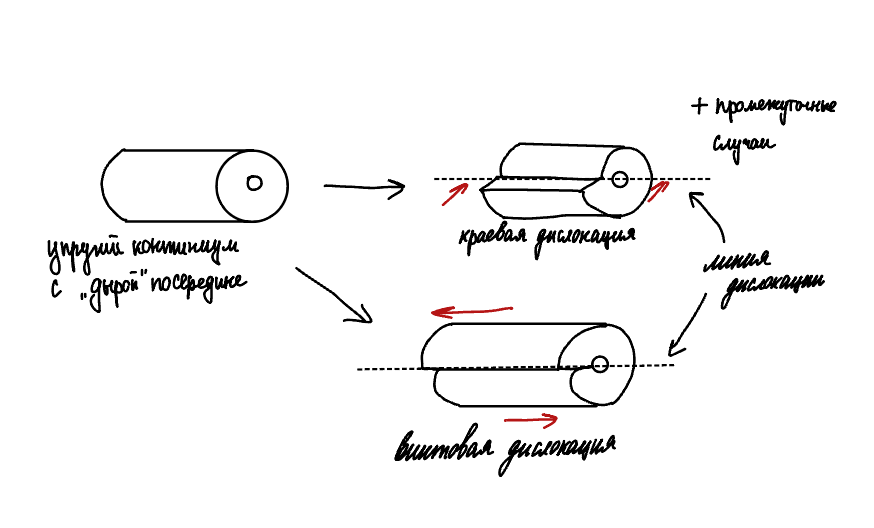
\includegraphics[width=0.55\textwidth]{volterra_dislocation.png}\caption{Дислокации Вольтерра} \label{fig:volterra_dislocation}
\end{figure} 
Сдвигом упругого континуума к оси цилиндра мы получаем краевую дислокацию, а сдвигом вдоль оси цилиндра - винтовую. Возможны и смешанные варианты.\par
Краевая дислокация представляет собой внедрение дополнительной атомной плоскости в кристалл (рис. \ref{fig:edge_dislocation}). Вдоль линии дислокации разупорядочение структуры максимально.
\begin{figure}[h!]
\centering
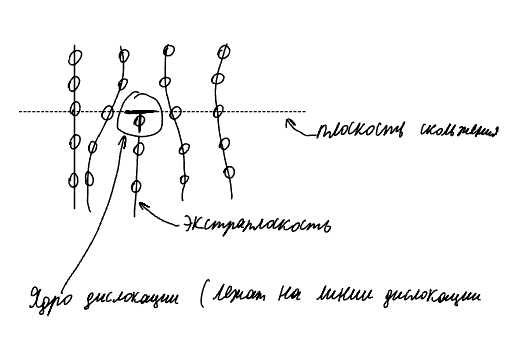
\includegraphics[width=0.55\textwidth]{edge_dislocation.png}\caption{Краевая дислокация}\label{fig:edge_dislocation}
\end{figure} 
\par
Дислокации удобно описывать при помощи вектора Бюргерса $\vec{b}$. Это вектор невязки между завершённым контуром в идеальном кристалле и аналогичным ему завершённым контуром, захватывающим дислокацию в реальном кристалле (рис. {\ref{fig:Burgers_vector}}).
\begin{figure}[h!]
\centering
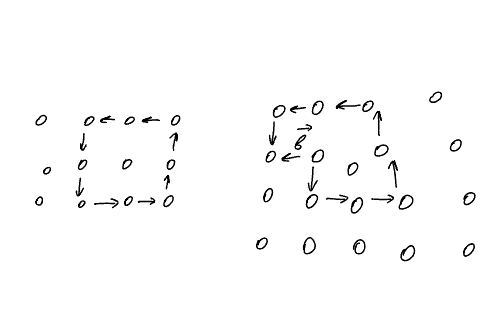
\includegraphics[width=0.55\textwidth]{Burgers_vector.png}\caption{К определению вектора Бюргерса} \label{fig:Burgers_vector}
\end{figure} 
\par
Краевая дислокация: $\vec{b}\perp$ линии дислокации\par
Винтовая дислокация: $\vec{b}\parallel$ линии дислокации\par
Вдоль линии дислокации $\vec{b}=const\Rightarrow$ дислокация не может оборваться внутри кристалла, должна либо замкнуться, либо расщепиться, либо выйти на поверхность.\par
Дислокации существенным образом искажают решётку, вызывая значительное поле напряжений и деформаций. Для винтовой дислокации 
\begin{equation}
    \varepsilon \sim \frac{b}{2\pi r}, \sigma \sim \frac{Gb}{2\pi r}
\label{eq:dislocation_force_field} %так как все билеты в последствии будут собираться в book, то картинки и ссылки должны называться осмысленно 
\end{equation}
В случае краевой дислокации возникает зависимость $\varepsilon$ и $\sigma$ от угла, хотя в целом $\varepsilon, \sigma \sim \frac{1}{r}$, то есть, поле затухает медленно.
\begin{equation}
   E_{\text{дислокации}}=E_{\text{ядра}}+E_{\text{упр}}
\label{eq:dislocation_energetics} 
\end{equation}
\begin{equation}
   E_{\text{упр}}=\frac{Gb^2}{4\pi}\ln \frac{r}{r_0} \text{ для винтовой дислокации}
\label{eq:screw_dislocation_energetics} 
\end{equation}
\begin{equation}
   E_{\text{упр}}=\frac{Gb^2}{4\pi(1-\nu)}\ln \frac{r}{r_0} \text{ для краевой дислокации}
\label{eq:edge_dislocation_energetics} 
\end{equation}
Здесь $\nu$ - коэффициент Пуассона, $r_0$ - размер ядра дислокации ($r_0 \sim 5-10 b$). \par
Плотность дислокаций определяется выражением \ref{eq:density_dislocation}:
\begin{equation}
   \rho=\frac{l}{V}
\label{eq:density_dislocation} 
\end{equation}
Здесь $l$ - полная длина дислокаций в образце объёмом $V$. В хорошо отожжённых металлах $\rho \sim 10^6-10^8$ см$^{-2}$. В полупроводниках $\rho \sim 10-10^5$ см$^{-2}$. После пластической деформации металла плотность дислокаций может достигать $\rho \sim 10^12-10^14$ см$^{-2}$. Для определения $\rho$ можно протравить шлиф, определить число ямок травимости - это точки выхода дислокаций на поверхность - и посчитать $\rho=\frac{N}{S}$.
\section{Плоское скопление дислокаций. Дефекты упаковки, двойниковые дефекты.
Оценка энергии дефекта упаковки по ширине растянутой дислокации}
\underline{Плоское скопление дислокаций} - это структура, представляющая собой n дислокаций, расположенных в одной плоскости скольжения перед дефектом, тормозящим скольжение дислокаций (напр. - граница зерна). Математическое описание такой структуры составляет суть задачи Набарро-Херринга. Можно получить, что положениям дислокаций в плоском скоплении соответствуют нули полинома Лагера. 
\begin{figure}[h!]
\centering
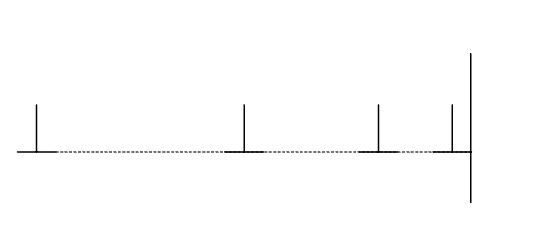
\includegraphics[width=0.55\textwidth]{dislocation_pile.png}\caption{Плоское скопление дислокаций}\label{fig:dislocation_pile}
\end{figure} 
\par Эта структура возникает вследствие отталкивания дислокаций одного знака. В головном скоплении на дислокацию действует сила $F=nF_d=n\tau b$, где $\tau$ - внешнее касательное напряжение, $b$ - вектор Бюргерса, $F_d$ - сила по формуле Мотта. \par
Это означает, что с ростом числа дислокаций существенно возрастает напряжение на границе зерна, так что при некотором значении $\tau$ дислокации начнут проскакивать через границу $\Rightarrow$ наблюдаем предел текучести на кривой нагружения. \par 
Можно получить, что число дислокаций $n\sim D \tau$, где $D$ - размер зерна. Тогда напряжение на границе $\tau^* = n\tau \sim D\tau^2$
\begin{equation}
  \Rightarrow \tau = \frac{k}{\sqrt{D}}+\tau_0
\label{eq:Hall-Petch} 
\end{equation}
Выражение \ref{eq:Hall-Petch} - это формула Холла-Петча. Описывает зависимость предела текучести в изотропном материале от размера зерна. Часто используется для оценки временного сопротивления разрыву. Слагаемое $\tau_0$ описывает порог напряжений, необходимый, чтобы сдвинуть ядро дислокации (т.н. Барьер Пайерлса).
\par
\underline{Дефект упаковки} - это нарушение порядка следования атомных слоёв в структуре. Например - отсутствие, или, наоборот, дополнительный слой в ГЦК: \par АВСАB:ABC - дефект вычитания 
\par АВСА\textbf{С}ВСАВС - дефект внедрения
\par Образование дефекта упаковки можно описать в терминах частичных дислокаций. Полная краевая дислокация в ГЦК обладает двойной экстраплоскостью, так что при её скольжении в плоскости {111} последовательность укладки слоёв не нарушается (рис. \ref{fig:partial_dislocation}). 
\begin{figure}[h!]
\centering
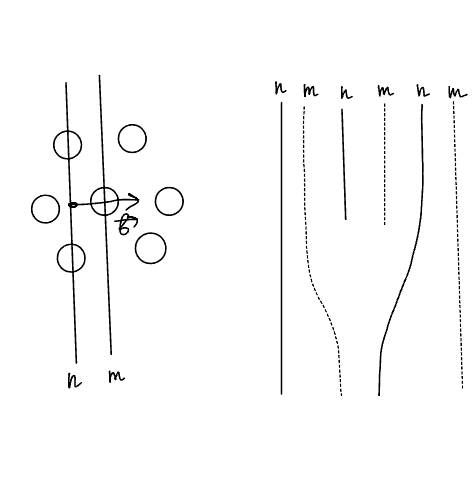
\includegraphics[width=0.55\textwidth]{partial_dislocation.png}\caption{Строение и перемещение краевой дислокации в ГЦК}\label{fig:partial_dislocation}
\end{figure} 
\begin{figure}[h!]
\centering
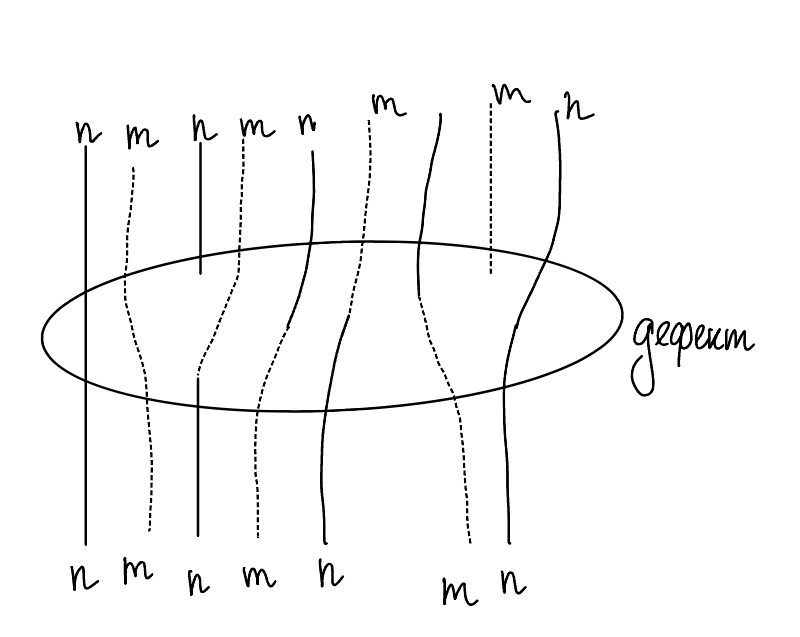
\includegraphics[width=0.55\textwidth]{partial_dislocation_full_view.png}\caption{Дефект упаковки между двумя частичными дислокациями} \label{fig:partial_dislocation_full_view}
\end{figure} 
При движении полной дислокации атомы смещаются между симметрически эквивалентными положениями в структуре. Однако атомы экстраплоскости могут начать перемещаться, "перекатываясь" между ложбинками в укладке слоя. В результате нарушается порядок следования слоёв, образуется дефект упаковки, ограниченный двумя частичными дислокациями (рис. \ref{fig:partial_dislocation_full_view}) с нетрансляционными векторами Бюргерса:
\begin{equation}
  \vec{b}=\vec{b_1}+\vec{b_2}, \text{ }\vec{b_1}\widehat{  }\text{ }\vec{b_2} = 60^\circ
\label{eq:partial_dislocation} 
\end{equation}
Образование дефекта упаковки (т.н. растянутой дислокации) энергетически выгодно, суммарная энергия двух частичных дислокаций меньше, чем энергия одной краевой. Частичные дислокации отталкиваются, однако с увеличением размеров дефекта упаковки растёт его упругая энергия, в результате чего можно говорить о некотором "равновесном" размере дефекта. Упругую энергию дефекта упаковки можно оценить по формуле \ref{eq:Energy_mispacking}.
\begin{equation}
  \gamma = \sigma_1b_2= \frac{G(\vec{b_1},\vec{v_2})}{2\pi l (1-\nu)}
\label{eq:Energy_mispacking} 
\end{equation}
Здесь $\sigma_1$ - поле напряжений, создаваемое первой частичной дислокацией, $l$ - размер дефекта, $\nu$ - коэффициент Пуассона.
\par
\underline{Двойниковый дефект} - это зеркальное расположение атомных плоскостей относительно некоторой плоскости (т.н. двойниковой границы). Может возникать как в результате деформации хрупкого тела, так и непосредственно в ходе роста кристалла. Двойниковые границы называют специальными границами, искажения на таких границах минимальны, равно как и энергия таких границ.
\par ABCBA
\section{Взаимодействие различных дефектов. Модели строения границ зерен.
Сегрегация примесей в поликристаллическом материале.}
Точечные и протяжённые дефекты взаимодействуют друг с другом. Движущая сила этого взаимодействия - минимизация упругой энергии деформации кристаллической решётки. точечные дефекты притягиваются друг к другу. Соприкосновение вакансий выгодно, поскольку снижает число разорванных в веществе связей. Дефекты по Френкелю притягиваются, так как сближение двух пар "междоузельный атом + вакансия" позволяет уменьшить деформацию, создаваемую каждым дефектом в отдельности. Точечные дефекты (в т.ч. атомы примеси) имеют тенденцию скапливаться вблизи протяжённых дефектов в сильнодеформированных областях с образованием атмосферы Коттрелла вокруг дислокаций и атмосферы Судзуки вокруг дефектов упаковки. точечные дефекты могут осаждаться на экстраплоскость, вызывая её переползание перпендикулярно плоскости скольжения дислокации.
\par
Дислокации взаимодействуют друг с другом, знак этого взаимодействия определяется положением дислокаций друг относительно друга. Если поля напряжений и деформаций двух дислокаций гасят друг друга, то такое взаимодействие энергетически выгодно, дислокации притягиваются. В противном случае дислокации отталкиваются. В одной плоскости скольжения дислокации одного знака отталкиваются, разных знаков - притягиваются. Возможны устойчивые конфигурации дислокаций - например, плоское скопление или стенка дислокаций (рис. \ref{fig:dislocation_configurations}).
\begin{figure}[h!]
\centering
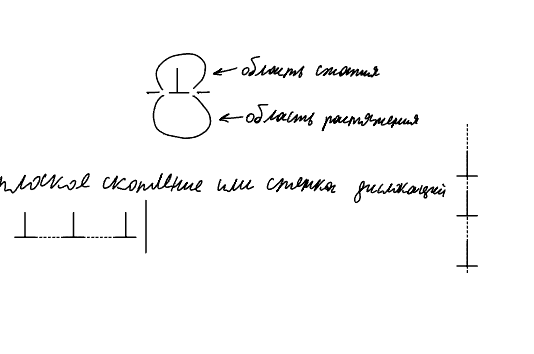
\includegraphics[width=0.55\textwidth]{dislocation_configurations.png}\caption{Примеры устойчивых конфигураций + напряжения вокруг краевой дислокации} \label{fig:dislocation_configurations}
\end{figure} 
\par
Стенка дислокаций фомрирует так называемую малоугловую границу между зёрнами кристалла. Это т.н. граница наклона, когда два зерна развёрнуты друг относительно друга на угол разупорядочения $\theta$ (рис. \ref{fig:misfit_angle}).

\begin{figure}[h!]
\centering
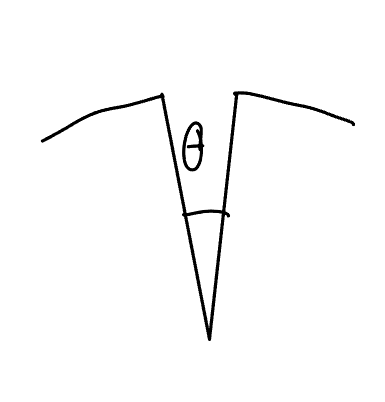
\includegraphics[width=0.3\textwidth]{misfit_angle.png}\caption{Угол разупорядочения} \label{fig:misfit_angle}
\end{figure} 
Существуют также малоугловые границы кручения, образованные серткой винтовых дислокаций. 
\par
При малых углах разориентировки для границ наклона справедлива формула Билби-Франка:
\begin{equation}
 h \approx \frac{b}{\theta}
\label{eq:Bilbi-Frank} 
\end{equation}
Здесь h -расстояние между соседними дислокациями в стенке. При малых $\theta < 15^\circ$ h велико, и ядра дислокаций не перекрываются. Удельная поверхностная энергия такой границы может быть описана формулой 
\begin{equation}
\gamma = \frac{Gb\theta}{4\pi (1-\nu)} \left(\ln \frac{b}{r_0} - \ln \theta \right)
\label{eq:boundary_energetics} 
\end{equation}
Для высокоугловых границ эта модель неприменима, энергия границы зависит от угла, как показано на рис. \ref{fig:boundary_energetics}.
\begin{figure}[h!]
\centering
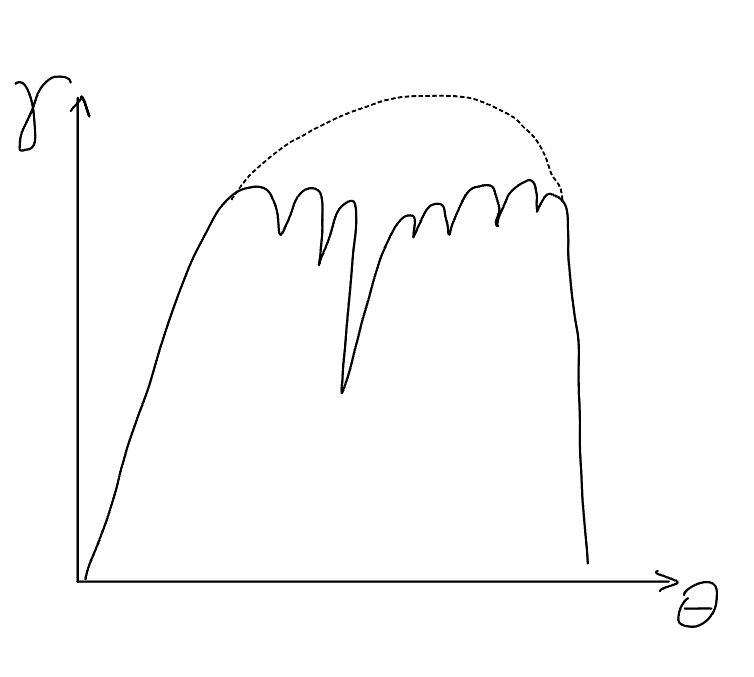
\includegraphics[width=0.3\textwidth]{boundary_energetics.png}\caption{Энергия границы} \label{fig:boundary_energetics}
\end{figure} 
Резкие минимумы энергии отвечают специальным, двойниковым высокоугловым границам. На таких границах наблюдается \underline{решётка совпадающих узлов} с некоторым периодом n. Специальные границы обозначают символом $\Sigma n$, где n -период РСУ. Такое взаиморасположение зёрен требует значительно меньших деформаций, энергетически это выгодно. Между минимумами энергии расположены точки, соответствующие несовершенным высокоугловым границам, для них нет РСУ, просто часть узлов решётки должны совпасть. 
\par
Для описания высокоугловых границ часто используют понятие зернограничных дислокаций, обеспечивающих скольжение зёрен друг относительно друга. Строится решётка зернограничных сдвигов (часть узлов - пусты, в остальных узлах - все атомы, и входящие в РСУ, и не входящие в РСУ). Зернограничные дислокации вводятся в этой решётке и перемещаются в ней. 
\par Вследствие расхождения кристаллических решёток, на границе зерён есть множество мест, в которых энергетически выгодно расположиться крупным примесным атомам (рис. \ref{fig:boundary_sites}).
\begin{figure}[h!]
\centering
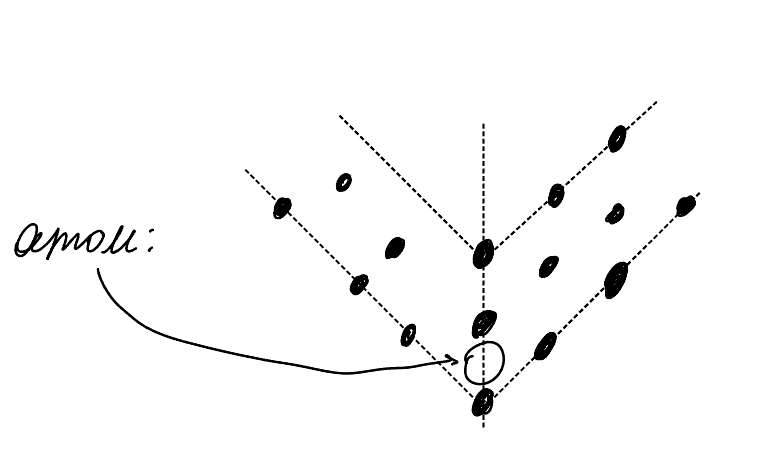
\includegraphics[width=0.3\textwidth]{boundary_sites.png}\caption{К размещению примеси на границе зерён} \label{fig:boundary_sites}
\end{figure} 
\par
Не все примеси склонны сегрегировать к границам зёрен (преимущественно располагаться на них), хотя большинство примесей сегрегирует к границе, такие примеси называют горофильными. Сегрегация примеси обычно описывается уравнением адсорбции Гиббса ($c_i$ - объёмная концентрация вблизи границы):
\begin{equation}
 \Gamma_i = - \frac{c_i}{RT} \left(\frac{\partial \gamma}{\partial c_i} \right)_S
\label{eq:Gibbs_adsorbtion} 
\end{equation}
Чем хуже растворима примесь в веществе, тем сильнее она сегрегирует к границам зёрен. В рамках чисто упругой модели концентрация примеси вблизи границы рассчитывается по формуле 
\begin{equation}
 c_i=c_0e^{-\frac{E}{kT}} \text{, где } E\sim \varepsilon^2
\label{eq:elastic_model_concentrarion} 
\end{equation}
В более сложной модели среднего поля учитывается взаимодействие атомов примеси друг с другом. В этом случае используется изотерма Гугенхейма-Фаулера:
\begin{equation}
 \frac{x}{1-x} = \frac{c_0}{1-c_0}\exp (-\frac{\Delta f +2z\theta x}{kT})
\label{eq:elastic_model_concentrarion}  
\end{equation}
Здесь x - доля занятых позиций на границе, z - КЧ на границе, $\theta = \frac{1}{2} (E^{BB} + E^{AA} - 2E^{AB})$, $\Delta f$ - энергия обмена атомом А на границе с атомом В в объёме. \par
В случае сильного взаимодействия атомов примеси может наблюдаться образование разных поверхностных фаз, напр. - кластеров.
\section{Механизмы зарождения и размножения дислокаций. Механизмы
пластической деформации и разрушения материалов} 
1) Дислокации могут возникать вследствие пластической деформации кристалла. для того, чтобы породить дислокацию, необходимо преодолеть энергетический барьер Пайерлса. Для этого нужно приложить напряжение $\tau>\frac{Gb}{2\pi r_c}$, где $r_c$ - некоторый критический размер ядра дислокации, по достижении которого дислокация образуется.
\par 2) Дислокации могут порождаться вследствие структурного несоответствия двух контактирующих фаз (плёнка+подложка). Это так называемые дислокации несоответствия. Они возникают при превышении толщиной плёнки некоторого критического значения $h_c\approx \frac{b}{9.9 f}$, где $f=\frac{\Delta a}{a}$ - параметр несоответствия.
\par
3) Дислокации возникают при кристаллизации поликристалла с произвольной ориентацией центров кристаллизации вследствие структурного несоответствия на границах зёрен.
\par 4) дислокации могут размножаться, например -  по механизму источника Франка-Рида (рис. \ref{fig:Frank-Reed}). В качестве такого источника выступает закреплённая в двух точках дислокация. Она выгибается под действием внешнего напряжения, пока не примет форму полуокружности при напряжении $\tau \approx \frac{Gb}{L}$, где L - расстояние между точками закрепления.
\begin{figure}[h!]
\centering
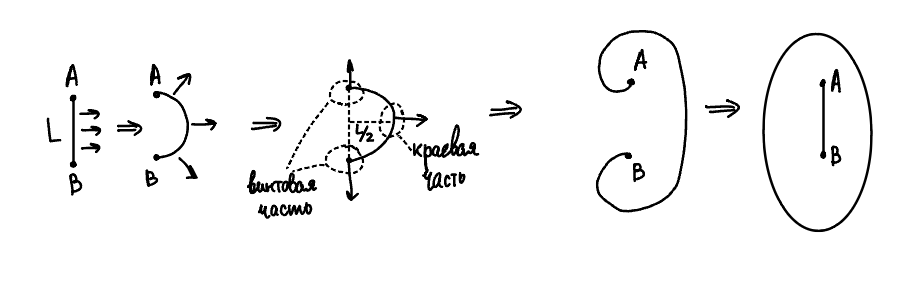
\includegraphics[width=0.9\textwidth]{Frank-Reed.png}\caption{Источник Франка-Рида} \label{fig:Frank-Reed}
\end{figure} 
После этого дислокация самопроизвольно расширяется, пока два участка петли не столкнутся и не с аннигилируют. В результате образуется дислокация между точками АВ и дислокационная петля вокруг источника. Эта петля распространяется по кристаллу, пока не выйдет на его поверхность.
\par
5) Также дислокации могут расщепляться с образованием полных или частичных дислокаций, либо возникать в результате столкновения частичных или полных дислокаций.
\par
Основной механиз пластической деформации - это скольжение дислокаций по плоскостям скольжения. В этом случае на поверхности деформируемого материала наблюдается серия полос (рис. \ref{fig:deformation_patterns}). Хрупкие материалы деформируются за счёт двойникования.
\begin{figure}[h!]
\centering
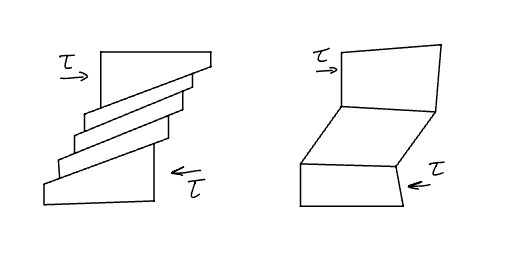
\includegraphics[width=0.5\textwidth]{deformation_patterns.png}\caption{Пластический (слева) и хрупкий (справа) деформацированный материал} \label{fig:deformation_patterns}
\end{figure} 
В случае пластической деформации по механизму скольжения дислокаций, могут активироваться разные системы скольжения. Число возможных систем скольжения определяется кристаллической структурой материала (12 в ГЦК, 3 или 6 в ГПУ). Чем больше возможных систем, тем пластичнее материал. Для каждой плоскости скольжения есть свой  предел текучести:
\begin{equation}
\tau_R = \sigma \cos \varphi \cos \lambda
\label{eq:Schmidt-Boas}  
\end{equation}
Это закон Шмида-Боаса (проекция внешнего напряжения на плоскость скольжения).
\begin{figure}[h!]
\centering
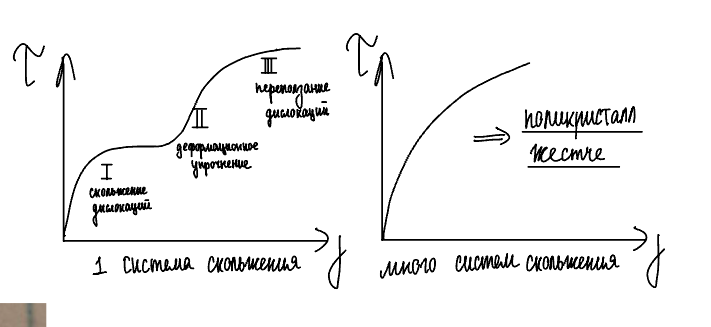
\includegraphics[width=0.7\textwidth]{tension_curve.png}\caption{Кривые нагружения для одной системы скольжения и многих систем скольжения (поликристалл)} \label{fig:tension_curve}
\end{figure} 
Деформационное упрочнение соответствует образованию плоских скоплений дислокаций вблизи границ зёрен.\par
При высоких температурах может наблюдаться  т.н. \underline{высокотемпературная ползучесть} (creep), когда при постоянной нагрузке происходит увеличение $\varepsilon$, поскольку диффузия облегчена (рис. \ref{fig:creep}).
\begin{figure}[h!]
\centering
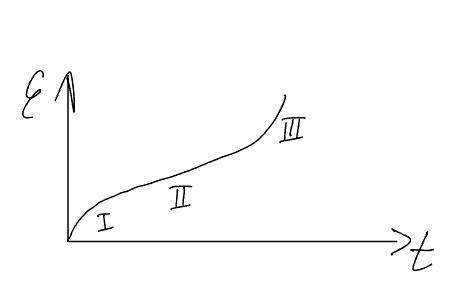
\includegraphics[width=0.3\textwidth]{creep.png}\caption{Зависимость деформации от времени} \label{fig:creep}
\end{figure} 
На рисунке \ref{fig:creep} область I соответствует неустановившейся ползучести (скольжение и генерации дислокации), область II - установившаяся ползучесть (генерация), III - переползание дислокаций, материал разрушается.
\par
В нанокристаллических материалах может наблюдаться сверхпластичность за счёт смещения зёрен друг относителньо друга. 
\par При существенном увеличении $\sigma$ в пластических материалах может наблюдаться диффузионная ползучесть Коббла (по границам зёрен), а при $T\uparrow \uparrow$ - ползучесть Набарро-Херринга, когда деформация происходит засчёт массопереноса в зерне. 
\par
\underline{Разрушение} материалов обычно протекает с образованием трещины. В пластичных материалах в области шейки копятся вакансии, образуются поры, сливаются в трещину, и происходит разрушение. Хрупкие тела разрушаются вокруг опасного дефекта (трещины), без образования шейки. Трещина - это концентратор напряжений, стремится раскрыться, чтобы снизить свою упругую энергию. Однако при раскрытии трещины повышается её поверхностная энергия, поэтому при относительно небольших напряжениях трещина достигает равновесного размера и далее не растёт.
\begin{equation}
\sigma_{\Gamma} = \sqrt{\frac{2E\gamma}{\pi a}}, \text{ где 2a - размер трещины, $\gamma$ - пов. плотн. энергии, Е - модуль Юнга}
\label{eq:Griffits}  
\end{equation}
Однако если в материале есть трещина длиной 2а, а приложенное напряжение превышает критическое напряжение по Гриффитсу ( ур. \ref{eq:Griffits}), то происходит резкий неконтролируемый рост трещины, материал разрушается. Прежде чем достигнуть критического размера, трещина медленно растёт за счёт эффекта среды - разрыва хим. связей в области трещины под малой нагрузкой. \par 
Зародиться трещина может вследствие столкновения дислокаций. 
\par Если материал подвергается знакопеременным нагрузкам, то возможно утсалостное разрушение. В этом случае сперва происходит рост усталостной трещины, например, по механизму Вуда (рис. \ref{fig:Wood_crack}). Трещина достигает критического размера, после чего происходит разрушение. Торец образца выглядит, как на рисунке \ref{fig:crack_fractography}.
\begin{figure}[h!]
\centering
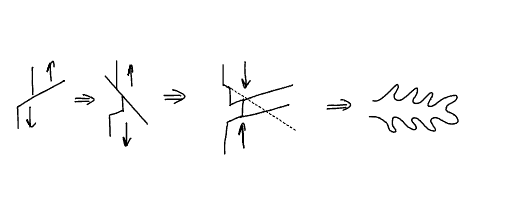
\includegraphics[width=0.7\textwidth]{Wood_crack.png}\caption{Механизм Вуда} \label{fig:Wood_crack}
\end{figure} 
\begin{figure}[h!]
\centering
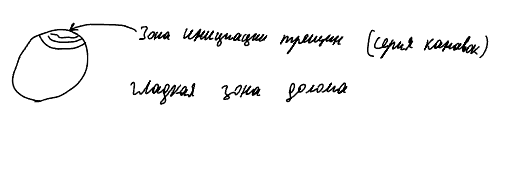
\includegraphics[width=0.7\textwidth]{crack_fractography.png}\caption{Шлиф образца, разрушенного по усталостному механизму}\label{fig:crack_fractography}
\end{figure} 
\section{Механизмы атомно-молекулярных процессов кристаллизации. Зависимости
скорости роста от величины пересыщения в случае нормального роста, спирального
роста (БКФ-механизм), механизма с образованием зародышей (ФКС-механизм).}
Выделяют 3 механизма атомно-молекулярных процессов кристаллизации:\par
1) нормальный рост (подошедшие к поверхности атомы сразу же садятся на шероховатости пов-ти)
\par 2) рост с образованием зародышей (ФКС-механизм, кристалл растёт слой за слоем)
\par3) спиральный рост (БКФ-механизм, атомы садяться во внутренние углы ступенек вышедшей на поверхность винтовой дислокации, кристалл растёт послойно с образованием ростового холма)
\par В случае нормального роста изменение энтропии при кристаллизации невелико, $\Delta_f S < R$. Для этого поверхность кристалла должна быть шероховатой на атомном уровне. Считая, что скорость роста определяется скоростью соударений атомов с поверхностью, можно получить следующее выражение для скорости роста:
\begin{equation}
v = \frac{D_L}{d}(1-e^{-\frac{\Delta G_f}{kT}})
\label{eq:Normal_growth}  
\end{equation}
Это уравнение Вилсона-Френкеля. Здесь $D_L$ - коэффициент диффузии, d - молекулярный/атомный диаметр, $\Delta G_f$ - энергия Гиббса кристаллизации. \par
При малых величинах переохлаждения оно может быть записано в виде 
\begin{equation}
v = \frac{D_L \Delta H_f}{dkT^2}\Delta T \sim \Delta T
\label{eq:Normal_growth_approximation}  
\end{equation}
В случае спирального роста, скорость роста 
\begin{equation}
u \sim f_g \left(1 - \exp \left(-\frac{\Delta H_f \Delta T}{T_m R T} \right) \right)
\label{eq:Spiral_growth}  
\end{equation}
где $f_g \approx \frac{\Delta T}{2 \pi T_m}$ - доля предпочтительных для зародышеобразования мест (сайтов). При малых $\Delta T$ скорость роста $u\sim\Delta T^2$\par
В случае ФКС-механизма (образование зародышей на поверхности, изменение энтропии при кристаллизации весьма велико), атомы могут садиться только в выборочных сайтах. Рост кристалла начинается только при достаточно больших пересыщениях, зависимость скорости роста от $\Delta T$ нелинейная.
\begin{figure}[h!]
\centering
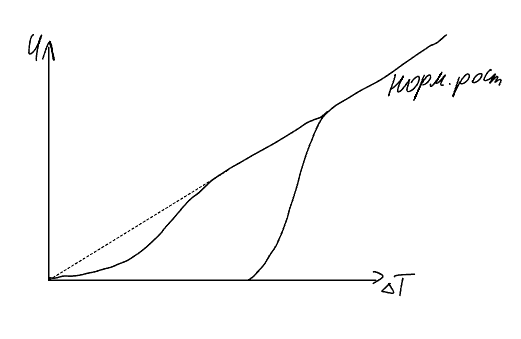
\includegraphics[width=0.4\textwidth]{crystal_growth.png}\label{fig:crystal_growth}\caption{Зависимость скорости роста кристалла от пересыщения для разных механизмов}
\end{figure}
\section{Развитие граней кристалла: теорема Гиббса-Вульфа, габитус кристалла с
точки зрения РВС-теории.}
Скорость роста граней кристалла может быть описана законом Браве: "скорость роста грани обратно пропорциональна плотности её узловой сетки". Огранка кристалла определяется гранями с наименьшими скоростями роста. Быстрорастущие грани как бы <<вытягивают>> медленные (рис. \ref{fig:edge_growth}). Медленнорастущие грани обладают малыми значениями индексов Миллера hkl.
\begin{figure}[h!]
\centering
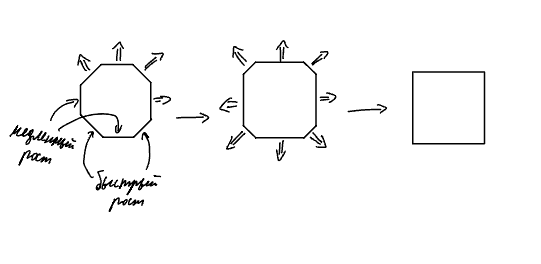
\includegraphics[width=0.5\textwidth]{edge_growth.png}\caption{Влияние скорости роста граней на огранку кристалла}\label{fig:edge_growth}
\end{figure}
Можно рассмотреть термодинамически равновесную огранку кристалла. Для этого решается вариационная задача по минимизации энергии Гиббса образующегося кристалла. В результате можно получить, что
\begin{equation}
\frac{\sigma_i}{r_i} = const \text{ для каждой грани}
\label{eq:Gibbs-Woolf_theorem}  
\end{equation}
Здесь $r_i$ - расстояние от центра кристалла до i-й грани, $\sigma_i$ - удельная поверхностная энергия грани. Это условие носит название \underline{теоремы Гиббса-Вульфа}.\par
В то же время в условиях относительно больших пересыщений включается не термодинамический, а кинетический контроль, существенную роль начинает играть шероховатость растущей грани, определяющая механизм и, следовательно, скорость её роста. Реальная огранка кристалла может отличаться от равновесной. Для описания кинетически контролируемого роста кристаллов построена теория периодической цепи связей (PBC-Theory). В структуре растущего кристалла можно выделить цепочки наиболее интенсивных химических связей, так называемые PBC-цепочки. Чем больше PBC-цепочек в грани, тем более гладкой является грань. Вводится классификация граней:
\par
1) 2 и более PBC-цепочки $\Rightarrow$ F-грани, гладкие, медленнорастущие (ФКС-механизм)
\par
2) 1 PBC-цепочка $\Rightarrow$ S-грани, менее гладкие, реже встречаются в огранке, ибо растут быстрее
\par
3) ни одной PBC-цепочки $\Rightarrow$ K-грани, высокошероховатые, быстро растут по нормальному механизму, в огранке не встречаются.
\begin{figure}[h!]
\centering
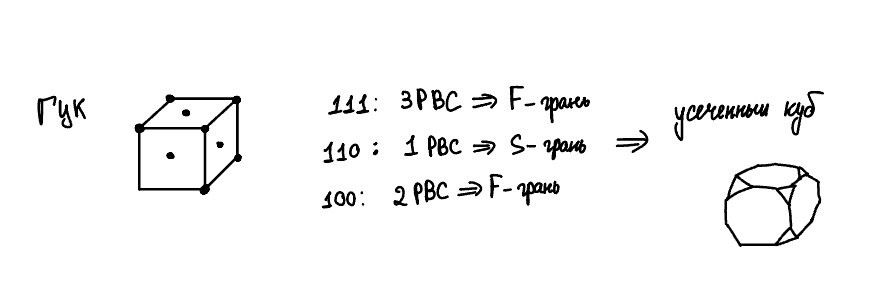
\includegraphics[width=0.7\textwidth]{example_PBC_theory.png}\caption{Пример применения PBC-теории для оценки огранки кристалла} \label{fig:example_PBC_theory}
\end{figure}
\section{Термодинамика выделения фазы, принцип Данкова-Конобеевского.
Гетерогенное зародышеобразование. Переохлаждение и кривизна ростового фронта}
Выделение новой фазы - это фазовый переход I рода, сопровождается скачком первых производных термодинамических потенциалов по интенсивным параметрам:
\begin{equation}
\left(\frac{\partial G}{\partial T}\right)_p = -S; \quad \left(\frac{\partial G}{\partial p}\right)_T = V 
\label{eq:first_derivatives_G_S}  
\end{equation}
Движущая сила процесса - минимизация энергии Гиббса системы. При этом может наблюдаться образование метастабильных фаз, если кинетический фактор (энергетический барьер, связанный с перестройкой структуры) играет значительную роль. Это так называемое правило ступеней Оствальда. 
\par
Изменение энергии Гиббса складывается  из объёмной, поверхностной и упругой составляющих:
\begin{equation}
\Delta G = \underset{<0}\Delta G_{\text{объёмн.}} + \underset{>0}\Delta G_{\text{ поверхн.}} + \underset{>0}\Delta G _{\text{упр.}}
\label{eq:DeltaG_phase_transitions}  
\end{equation}
Поскольку образование новой фазы неизбежно связано с возникновением новых границ раздела, $\Delta G_{\text{поверхн.}}>0$. Для минимизации вклада поверхностной энергии зерно новой фазы стремится к такой ориентации по отношению к исходной фазе, чтобы  рассогласование кристаллических решёток было минимальным. В этом и заключается так называемый \underline{принцип Данкова-Конобеевского}. При образовании новой фазы из расплава $\Delta G_{\text{упр.}}=0$, поэтому конкурируют только объёмная и поверхностная энергии. В случае \underline{гетерогенного зародышеобразования} в системе изначально присутствуют поверхности, обладающие избытком свободной энергии. В результате $\Delta G_{\text{поверхн.}}$ меньше, чем в случае гомогенного зародышеобразования, и рост кристаллов происходит при меньших значениях переохлаждения $\Delta T$.
\par
При гомогенном зародышеобразовании $\Delta G_{\text{объёмн.}}$ не сразу может преодолеть вклад от $\Delta G_{\text{поверхн.}}$, в результате зародыш обладает избытком энергии Гиббса, и кристаллизация идёт через потенциальный барьер (см. рис. \ref{fig:crystallization_barrier}):
\begin{equation}
\Delta G_c \sim \frac{1}{\Delta T}, r_c \sim \frac{1}{\Delta T}
\label{eq:crystallization_energy_barrier}  
\end{equation}
\begin{figure}[h!]
\centering
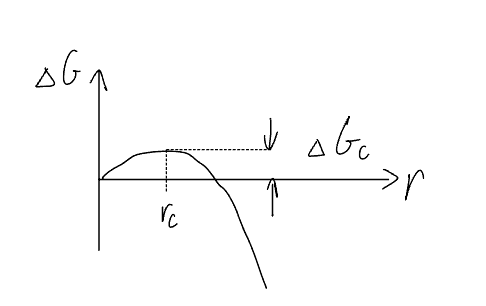
\includegraphics[width=0.3\textwidth]{crystallization_barrier.png}\caption{Потенциальный барьер кристаллизации} \label{fig:crystallization_barrier}
\end{figure}
$r>r_c \Rightarrow$ кристалл растёт, $r<r_c \Rightarrow$ зародыш растворяется.
\par При гетерогенном зародышеобразовании $r_c$ не меняется, а величина барьера уменьшается и становится равной
\begin{equation}
\Delta G_{het} = \Delta G_c (2-3\cos \theta + \cos^3\theta)
\label{eq:heterocrystallization_energy_barrier}  
\end{equation}
Здесь $\theta$ - это угол смачивания между зародышем и подложкой. Необходимо добиться такой величины $\Delta T$, чтобы случайно образующиеся зародыши могли вырасти.
\par
В то же время, высокие значения $\Delta T$ способны привести к нестабильности ростового фронта. Для роста искривлённой поверхности требуется меньшее пересыщение, чем для роста прямой поверхности. Малые выступы, образующиеся на ростовом фронте, превышают критический размер и начинают расти, поверхность роста искривляется. Чем сильнее изгибается фронт, тем меньшие переохлаждения требуются для его дальнейшего роста. Соответственно, тем больше получается актуальное переохлаждение вблизи границы. В результате происходит рост дендритов (рис. \ref{fig:dendrites_growth}) с последующим отрывом их от ростовой поверхности кристалла. Процесс нежелательный.
\begin{figure}[h!]
\centering
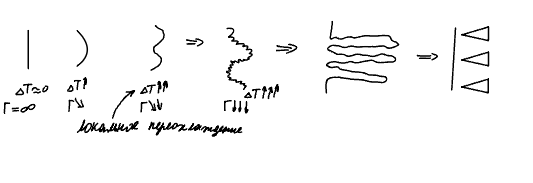
\includegraphics[width=0.85\textwidth]{dendrites_growth.png}\caption{Рост дендритов} \label{fig:dendrites_growth}
\end{figure}
\section{Распределение примеси по длине растущего из расплава кристалла.
Техническое оформление основных методов роста кристаллов из расплава.}
Вследствие несовпадения составов расплава и растущего кристалла (линии ликвидуса и солидуса на фазовой диаграмме не совпадают), состав расплава по мере роста кристалла непрерывно меняется (рис. \ref{fig:liquation_crystal_growth}). 
\begin{figure}[h!]
\centering
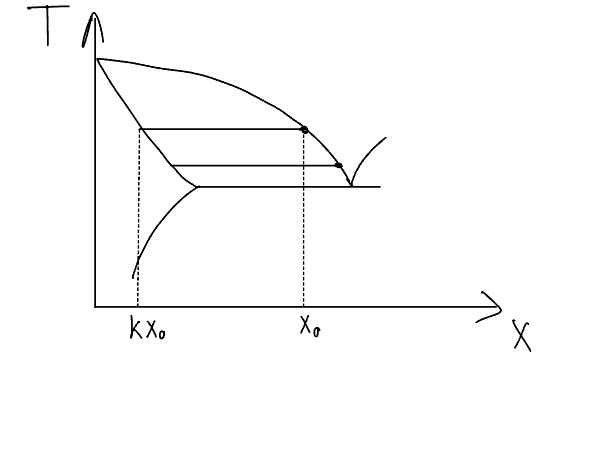
\includegraphics[width=0.3\textwidth]{liquation_crystal_growth.png}\caption{Причина непостоянства концентрации примеси в кристалле}\label{fig:liquation_crystal_growth}
\end{figure}
\begin{figure}[h!]
\centering
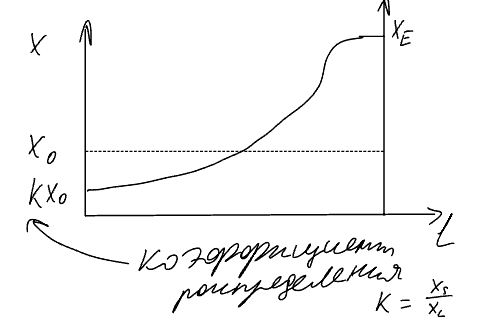
\includegraphics[width=0.5\textwidth]{c(x)_crystal.png}\caption{Зависимость концентрации примеси в кристалле от координаты}\label{fig:c(x)_crystal}
\end{figure}
В результате непрерывно меняется и состав растущего кристалла, так что в конечном итоге распределение примеси по кристаллу имеет вид, показанный на рис. \ref{fig:c(x)_crystal}. 
\par Коэффициент распределения $k=\frac{x_s}{x_L}\approx const$ для линейных ликвидуса и солидуса. Вид кривой x(l) получается при интегрировании выражения 
\begin{equation}
(x_L-x_S)df_S=(1-f_S)dx_L \text{   - принцип сохранения примеси}
\label{eq:impurity_conservation}  
\end{equation}
Здесь $f_S$ - объёмная доля кристалла (по сути - координата границы раздела). В результате получаем уравнение темпа кристаллизации:
\begin{equation}
x_S = kx_0 (1-f_S)^{k-1} = kx_0 (1-l)^{k-1} 
\label{eq:crystallization_rate}  
\end{equation}
Для того, чтобы избежать столь существенных неоднородностей состава (рис. \ref{fig:c(x)_crystal}), можно осуществлять подпитку расплава примесью, загружая в расплав шихту смеси компонентов состава $x_0$. В этом случае с учётом диффузии в расплаве получаем следующее распределение примеси по расплаву (рис. \ref{fig:c(x)_fusion}):
\begin{figure}[h!]
\centering
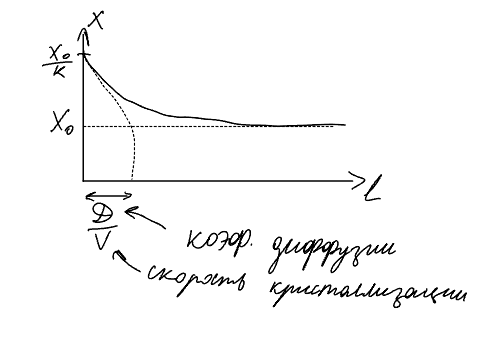
\includegraphics[width=0.5\textwidth]{c(x)_fusion.png}\caption{Зависимость концентрации примеси в расплаве от координаты}\label{fig:c(x)_fusion}
\end{figure}
\parИ, как следствие, такое распределение примеси по кристаллу (рис \ref{fig:c(x)_crystal_normal}):
\begin{figure}[h!]
\centering
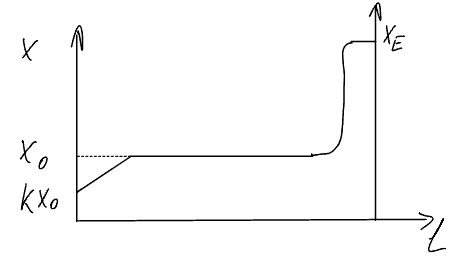
\includegraphics[width=0.5\textwidth]{c(x)_crystal_normal.png}\caption{Зависимость концентрации примеси в кристалле от координаты с учётом диффузии в расплаве}\label{fig:c(x)_crystal_normal}
\end{figure}
\par Начальная и конечная области отрезаются, остаётся однородный кристалл.
\par \underline{Основные методы роста кристаллов из расплава}:
\par 1) Бриджмен-Стокбаргер (движение расплава в температурном градиенте, рис. \ref{fig:Bridgeman_Stockbarger})
\par 2) Чохральский (вытягивание вращающейся затравки из расплава, рис. \ref{fig:Bridgeman_Stockbarger})
\par 3) Зонная плавка (рис. \ref{fig:zone_fusion})
\par 4) Вернейль (в пламени, для тугоплавких материалов, рис. \ref{fig:zone_fusion})
\par 5) Массовая и спонтанная кристаллизация 
\begin{figure}[h!]
\centering
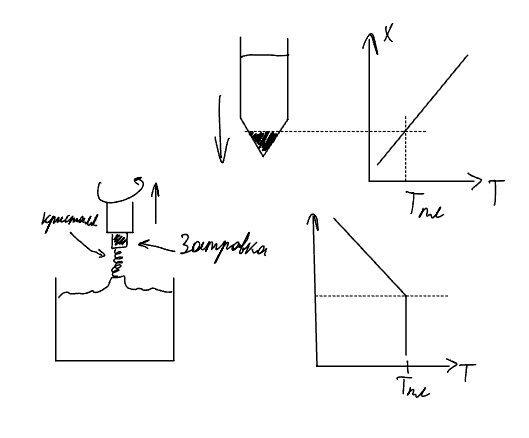
\includegraphics[width=0.4\textwidth]{Bridgeman-Stockbarger.png}\caption{Метод Бриджмена (сверху) и Чохральского (снизу)}\label{fig:Bridgeman_Stockbarger}
\end{figure}
\begin{figure}[h!]
\centering
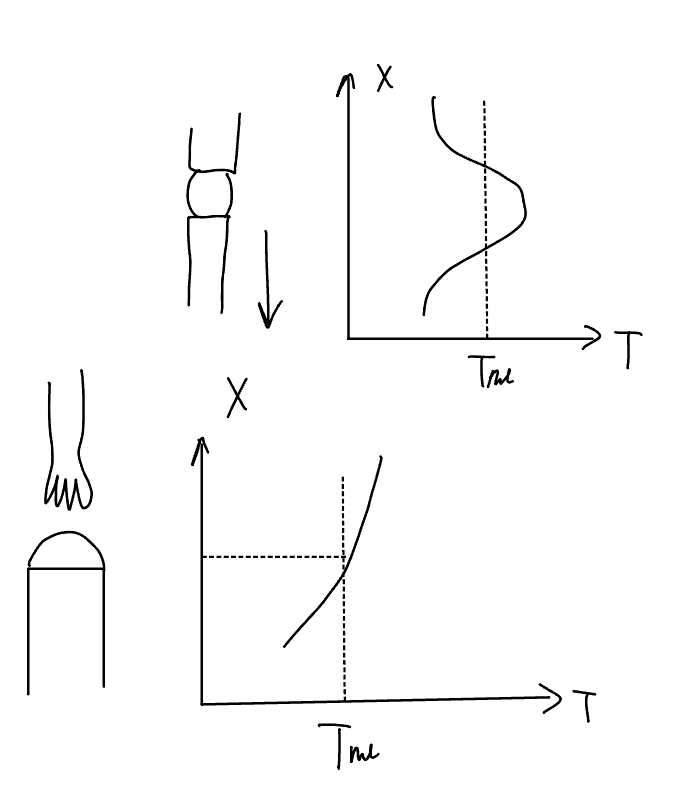
\includegraphics[width=0.4\textwidth]{zone_fusion.png}\caption{Метод зонной плавки (сверху) и Вернейля (снизу)}\label{fig:zone_fusion}
\end{figure}
\section{Направленная кристаллизация. Условие стабильности интерфейса при
направленной кристаллизации. Теория эвтектического роста.}
Направленная кристаллизация осуществляется следующим образом. на границу раздела кристалл/расплав подаётся температурный градиент, через который с некоторой скоростью v протягивается образец. v соответствует скорости кристаллизации. Важно, чтобы переохлаждение вблизи границы раздела было невелико, в противном случае можно получить нестабильность ростового фронта ($R\sim \frac{1}{\Delta T}$, R - радиус кривизны, $\Delta T$ - локальное переохлаждение). Для этого тепло должно отводиться через кристалл.
\par В случае направленной кристаллизации распределение примеси по расплаву имеет следующий вид (рис. \ref{fig:x(l)_crystal_melt}):
\begin{figure}[h!]
\centering
\centering
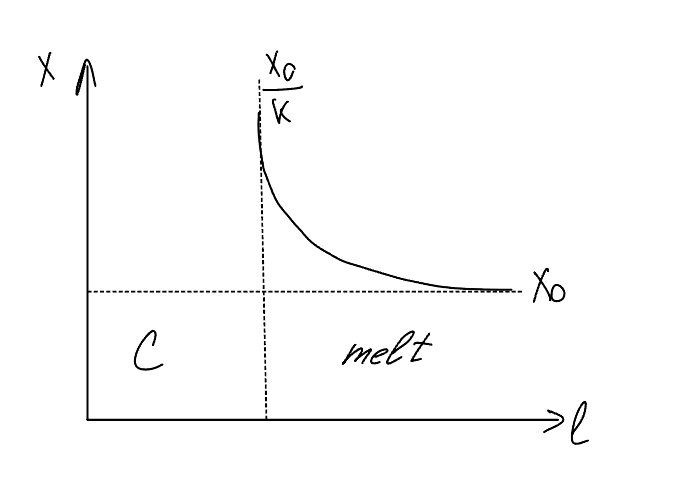
\includegraphics[width=0.2\textwidth]{x(l)_crystal_melt.png}\caption{Распределение примеси в кристалле и в расплаве вблизи границы раздела} \label{fig:x(l)_crystal_melt}
\end{figure}
\par  Каждой концентрации примеси можно сопоставить равновесную температуру, отвечающую данному составу на фазовой диаграмме. Если наложенный температурный градиент слишком мал (рис. \ref{fig:concentrational_undercooling}), то вблизи поверхности раздела раствор пересыщен, наблюдается так называемое концентрационное переохлаждение, которое способно привести к нестабильности ростового фронта точно также, как и обычное термическое. 
\begin{figure}[h!]
\centering
\centering
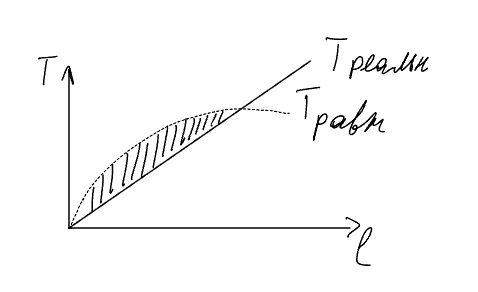
\includegraphics[width=0.3\textwidth]{concentrational_undercooling.png}\caption{К понятию концентрационного переохлаждения} \label{fig:concentrational_undercooling}
\end{figure}
\par Для стабильности ростового фронта важно, чтобы при росте кристалла скорость кристаллизации и температурный градиент были сбалансированы во избежание концентрационного переохлаждения. Условие стабильности ростового фронта записывается следующим образом:
\begin{equation}
\frac{\nabla T}{v}\geq \frac{-m_Lx_0(1-k)}{D_L} 
\label{eq:growth_stability}  
\end{equation}
Здесь $D_L$ - коэффициент диффузии в расплаве, $k=\frac{x_S}{x_L}$ - коэффициент распределения, $m_L<0$ - наклон ликвидуса (в линейной модели ликвидуса и солидуса).
\par
\underline{Кристаллизация эвтектик} описывается теорией Джексона-Ханта. В рамках этой теории распределение примеси по кристаллу описывается уравнением
\begin{equation}
\frac{\partial^2C}{\partial^2x}+\frac{\partial^2C}{\partial^2y}+\frac{v}{D}\frac{\partial C}{\partial z} = 0
\label{eq:Jackson-Hant_concentration}  
\end{equation}
Это означает, что распределение примеси по кристаллу в направлении z периодично. При кристаллизации эвтектики расплав пересыщен относительно обеих фаз сразу (рис. \ref{fig:eutectic_crystal}), так что обе фазы кристаллизуются одновременно с образованием стопки пластин-ламелей с дифференцировкой $\lambda$. 
\begin{figure}[h!]
\centering
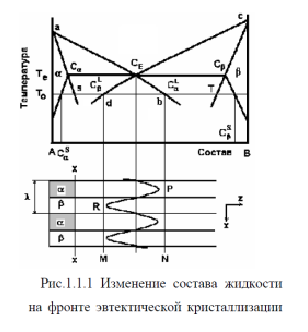
\includegraphics[width=0.5\textwidth]{eutectic_crystal.png}\caption{Переохлаждение и кристаллизация эвтектики}\label{fig:eutectic_crystal}
\end{figure}
\par Для того, чтобы движущая сила кристаллизации была отлична от нуля, требуется некоторое переохлаждение на границе, которое складывается из концентрационного переохлаждения (при образовании пластины одной фазы раствор обогащается вторым компонентом) и переохлаждения, связанного с кривизной ростового фронта:
\begin{equation}
\Delta T = Av\lambda + \frac{B}{\lambda}
\label{eq:eutectic_undercooling}  
\end{equation}
Первое слагаемое отвечает концентрационному переохлаждению, второе - переохлаждению за счёт кривизны ростового фронта.
\par Условие планарности ростового фронта эвтектического кристалла ($\Delta T \rightarrow min$): 
\begin{equation}
\lambda^2v=const
\label{eq:eutectic_planar_face1}  
\end{equation}
\begin{equation}
\frac{(\Delta T)^2}{v}=const
\label{eq:eutectic_planar_face2}  
\end{equation}
\begin{equation}
\Delta T \lambda = const
\label{eq:eutectic_planar_face3}  
\end{equation}
\section{Фазовые равновесия. Основные понятия: система, компонент, фаза,
степень свободы. Условия равновесия фаз. Правило фаз Гиббса. Фазовые
диаграммы Т-х двухкомпонентных систем.}
Фазовые равновесия - это равновесия между фазами в термодинамической системе. \underline{Термодинамическая система} - это материальный объект, выделенный из окружающей среды с помощью реально существующей или воображаемой границы. \underline{Компонентами} называют минимальный набор составляющих (реальные вещества/частицы, образующие систему), достаточный для описания состава системы.
\par
\underline{Пр.} $\rm CO, CO_2, O_2 \Rightarrow$ 3 составляющих, 2 компонента (ибо $\rm CO + \frac{1}{2}O_2=CO_2$)
\par
\underline{Фаза} - гомогенная часть гетерогенной системы, отделённая от других частей границей раздела, при переходе через которую свойства системы меняются скачком. \par
\underline{Степень свободы} - это параметр, который можно независимо менять, оставаясь при этом в пределах одной и той же фазы. Число степеней свободы (ЧСС) - количество таких независимых параметров.
\par С течением времени система может прийти в состояние термодинамического равновесия, когда внутри системы  не будет наблюдаться потоков вещества и энергии, и характеристики системы станут постоянными. В этом случае для фаз, составляющих систему, можно записать частные условия равновесия:
\begin{equation}
T^\alpha=T^\beta; p^\alpha = p^\beta; \mu_i^\alpha = \mu_i^\beta
\label{eq:partial_equilibrium_conditions}  
\end{equation}
То есть, во всех фазах должно соблюдаться равенство температур (термическое равновесие), давлений (механическое равновесие) и химических потенциалов каждого из компонентов (химическое равновесие). 
\par Правило фаз Гиббса связывает число степеней свободы $f$ с количеством равновесных фаз Ф в К-компонентной системе:
\begin{equation}
f=K-\Phi+N
\label{eq:Gibbs_rule}  
\end{equation}
Здесь N - число внешних управляющих факторов (p, T, $\vec{B}$, $\vec{g}$...). Обычно N=2, так как ключевую рлль играют p и Т.
\par ДЛя описания двухкомпонентных систем часто прибегают к использованию Т-х диаграмм, представляющих собой сечения р-Т-х диаграмм при постоянном давлении (обычно 1 атм.). В этом случае $f=K-\Phi+1$. Общий вид Т-х диаграммы показан на рисунке \ref{fig:T-x_diagram}.
\begin{figure}[h!]
\centering
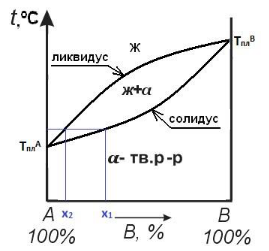
\includegraphics[width=0.3\textwidth]{T-x_diagram.png}\caption{Фазовая диаграмма двухкомпонентной системы}\label{fig:T-x_diagram}
\end{figure}
Для примера приведена Т-х диаграмма, описывающая систему двух неограниченно растворимых друг в друге компонентов. В областях ж и $\alpha$ $\Phi=1 \Rightarrow f=2$, можно менять Т и состав. В области двухфазного равновесия $f=1$, независимо можно менять только температуру, составы фаз жёстко связаны друг с другом.
\section{Основные виды конгруэнтных и инконгруэнтных равновесий. Правило
рычага. Способы графического изображения фазовых диаграмм
трехкомпонентных систем. Квазибинарные разрезы. Принцип триангуляции.} 
Равновесие называется конгруэнтным, если составы равновесных фаз совпадают. В противном случае равновесие называют инконгруэнтным. Трёхфазные равновесия делят на два больших типа: эвтектические (фаза при охлаждение распадается на две) и перитектический (фаза при нагревании распадается на две). В зависимости от состояния фаз (тв., ж., г.) различают следующие равновесия (рис. \ref{fig:phase_equilibrium_types}):
\begin{figure}[h!]
\centering
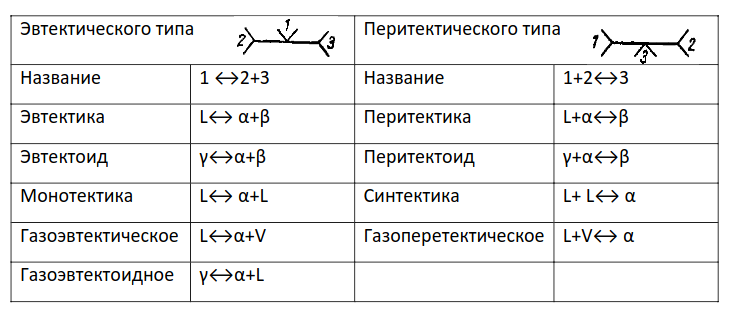
\includegraphics[width=0.8\textwidth]{phase_equilibrium_types.png}\caption{Типы трёхфазных равновесий}\label{fig:phase_equilibrium_types}
\end{figure}
\par Правило рычага позволяет найти соотношение между количеством двух равновесных фаз и их составом (рис. \ref{fig:lever_rule}, n - количество фазы, моль. x - мольная доля одного из компонентов):
\begin{figure}[h!]
\centering
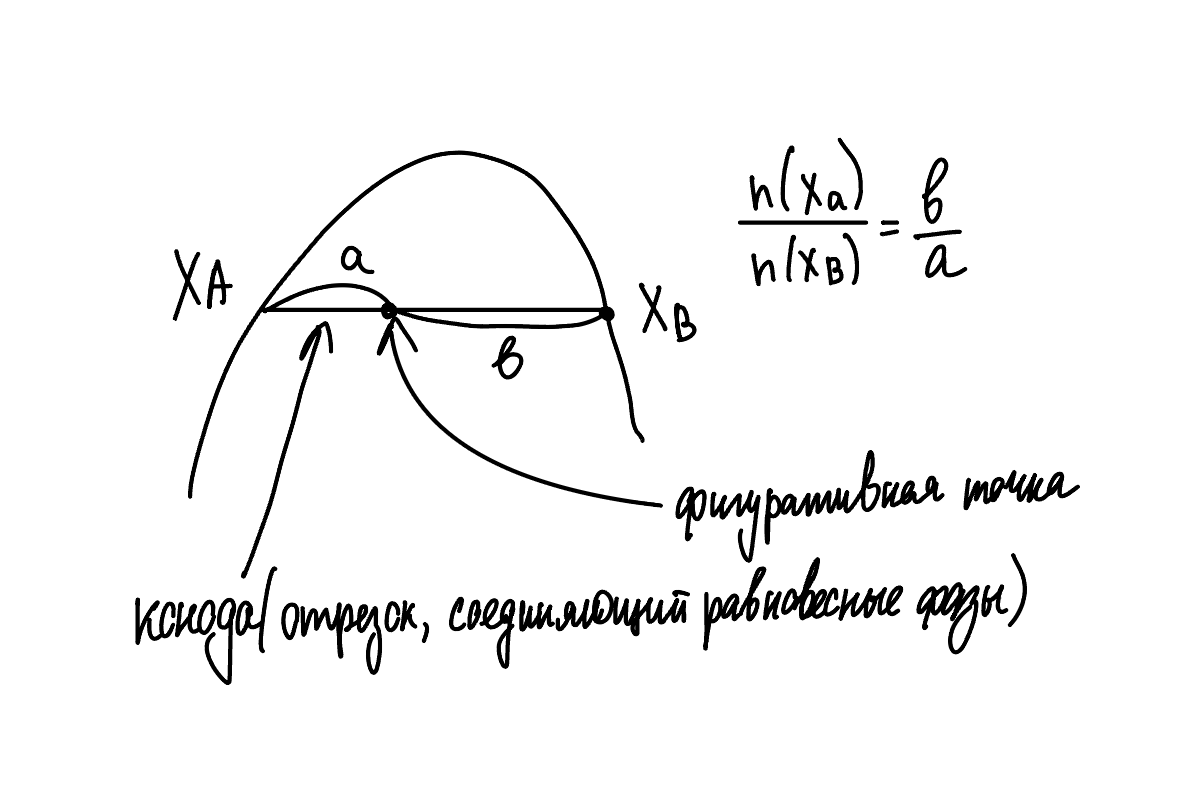
\includegraphics[width=0.6\textwidth]{lever_rule.png}\caption{Правило рычага}\label{fig:lever_rule}
\end{figure}
\par Для изображения фазовых диаграмм трёхкомпонентых систем часто используют треугольник составов Гиббса-Розенбома, который помещают в основание трёхмерной Т-х1-х2-х3 диаграммы при р=const (обычно 1 атм.). Чаще всего пользуются изотермическими сечениями таких диаграмм. Ещё используют развёртки трёхмерных диаграмм, а также их политермические разрезы. 
\par \underline{Квазибинарный разрез} - это политермический разрез, построенный вдоль отрезка, соединяющего на треугольнике составов два конгруэнтно плавящихся соединения, сосуществующих в данной системе (рис. \ref{fig:quasibinary}).
\begin{figure}[h!]
\centering
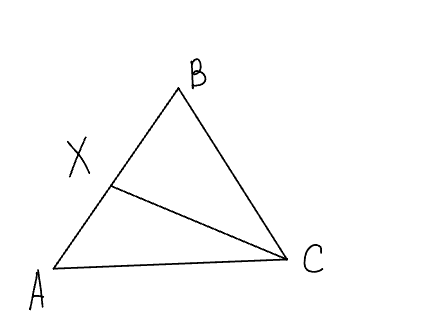
\includegraphics[width=0.3\textwidth]{quasibinary.png}\caption{Квазибинарный разрез}\label{fig:quasibinary}
\end{figure}
\par Можно показать, что смешением С и Х можно получить только точки, принадлежащие отрезке СХ, так что квазибинарное сечение по сути представляет собой двухкомпонентную фазовую диаграмму. При этом важно, чтобы фазы С и Х могли сосуществовать пр данных условиях (т.н. термодинамический критерий выбора квазибинарного разреза). В отдельных случаях при превышении некоторого температурного предела квазибинарный разрез может перестать быть таковым, ибо пройдут процессы химического превращения С и Х с образованием новых фаз.
\par Для изотермических сечений используется принцип триангуляции. Поскольку $p=const, T=const$, то $f=K-\Phi \Rightarrow max\Phi=K=3$. Это означает, что в равновесии может находиться не более трёх фаз. Если в результате некоторого процесса в системе К1-К2-К3 (рис. \ref{fig:triangulation}) получен образец (точка М), содержащий фазы А,В и С, отвечающие некоторым конгруэнтно плавящимся соединениям, присутствующим в данной системе, то треугольник АВС представляет собой область нонвариантного равновесия и не содержит иных фаз, кроме А, В и С. 
\par Такой подход к изучению фазовых диаграмм позволяет разбивать их на простейшие треугольники с тройной эвтектикой, проводить триангуляцию. Этот метод требует больших временных затрат, но позволяет максимально подробно описывать систему.
\begin{figure}[h!]
\centering
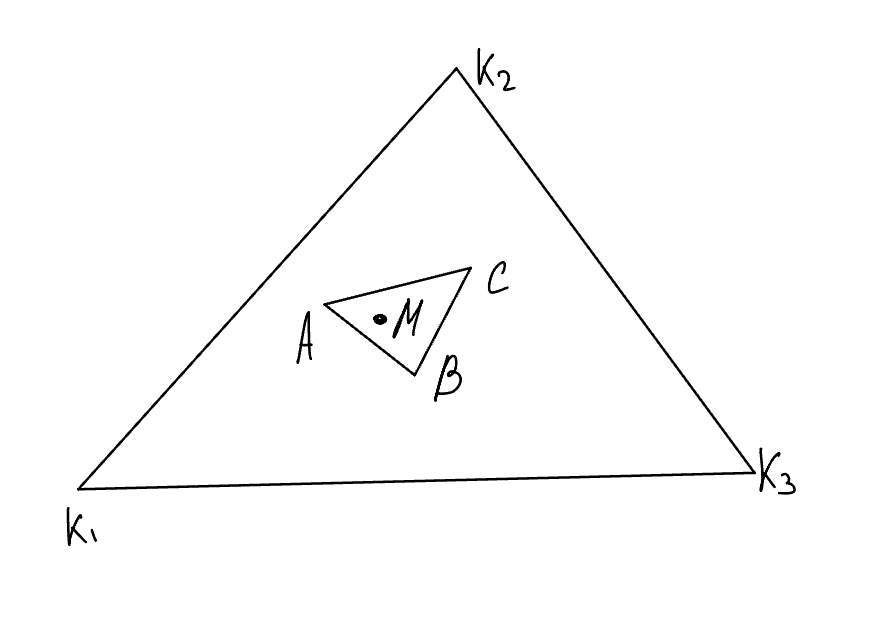
\includegraphics[width=0.4\textwidth]{triangulation.png}\caption{Процесс триангуляции} \label{fig:triangulation}
\end{figure}
\section{Фазовая диаграмма и микроструктура материала. Микроструктура
эвтектических и перитектических композитов. Ликвация и ее влияние на
микроструктуру материала}
По фазовой диаграмме системы можно понять последовательность процессов, происходящих при охлаждении расплава заданного состава $x_0$. Например, если кристаллизация проводится в системе с эвтектикой по пути, показанному на рис. \ref{fig:crystallization_path_eutectic}, то сперва кристаллизуются зёрна фазы $\alpha$, причём состав зерна меняется от ядра к поверхности.
\begin{figure}[h!]
\centering
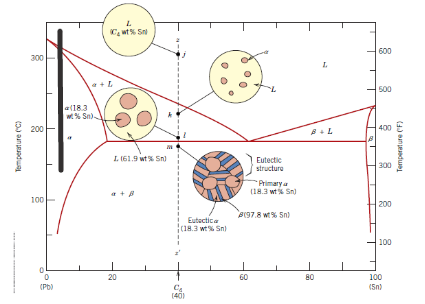
\includegraphics[width=0.6\textwidth]{crystallization_path_eutectic.png}\caption{Кристаллизация сплавов в системе с эвтектикой}\label{fig:crystallization_path_eutectic}
\end{figure}
По достижении температуры эвтектики между зёрнами фазы $\alpha$ кристаллизуется композит эвтектического состава. В результате сплав обладает микроструктурой, показанной на рис. \ref{fig:crystallization_path_eutectic} и характеризуется повышенной прочностью. 
\par
Если кристаллизацию вести по другому пути (рис. \ref{fig:crystallization_path_eutectic}, жирная чёрная линия слева), то будет получен однофазный пластичный материал из зёрен фазы $\alpha$. Если кристаллизуется эвтектический состав, будет получен чисто эвтектический композит \textit{(микроструктура как на рисунке, только без зёрен фазы $\alpha$, просто пластинки в зёрнах)}
\par
Если в системе есть перитектическое равновесие (например - перитектоид, как на рис. \ref{fig:crystallization_path_peritectic}), то по мере охлаждения расплава сперва будут образовываться зёрны фазы $\alpha$, а затем в них произойдёт выделение мелких зёрен фазы $\beta$, в результате чего прочность материала вырастет, а микроструктура будет иметь вид, показанный на рис. \ref{fig:crystallization_path_peritectic}.
\begin{figure}[h!]
\centering
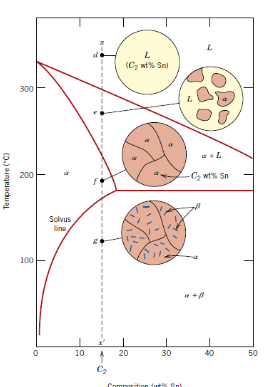
\includegraphics[width=0.4\textwidth]{crystallization_path_peritectic.png}\caption{Кристаллизация сплавов в системе с перитектоидом}\label{fig:crystallization_path_peritectic}
\end{figure}
\par Вследствие несовпадения составов расплава и растущего кристалла (линии солидуса и ликвидуса не совпадают) состав кристалла по мере роста непрерывно меняется (рис. \ref{fig:liquation}).
\begin{figure}[h!]
\centering
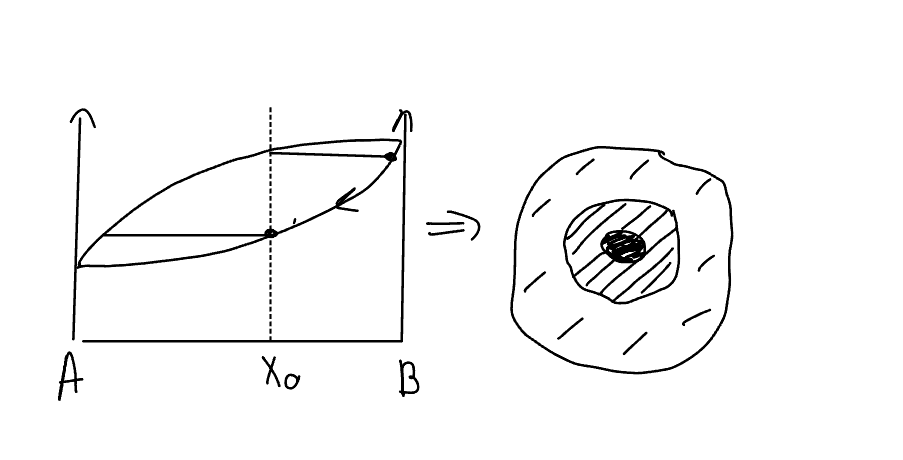
\includegraphics[width=0.8\textwidth]{liquation.png}\caption{Ликвация}\label{fig:liquation}
\end{figure}
В результате ядро зерна обогащено компонентом В, а внешняя область - обеднена, чтобы в среднем состав соответствовал $x_0$. Неоднородность распределения примеси, вызванная различной растворимостью примеси в кристалле и расплаве, наз. ликвацией. Особенно заметно это явление в массивных отливках, где кристаллизация идёт от стенок и дна формы к верхней части. Ликвация приводит к снижению прочности материала, бороться с ней можно путём диффузионного отжига либо замедленного литья.
\section{Закалка без полиморфного превращения. Закалка на мартенсит.
Кристаллогеометрия и термодинамика мартенситного превращения.}
Закалка без полиморфного превращения - это резкое охлаждение образца, при котором замораживаются диффузионные процессы и фиксируется высокотемпературный фазовый и химический состав, а также распределение дефектов. Для достижения этого эффекта металлические сплавы обычно закаляют со скоростями $\sim 1000 ^\circ C/\text{сек}$. для сохранения метастабильной аморфной структуры стекла требуются значительно меньшие скорости закалки. Закалка, проводимая непосредственно из расплава, позволяет избежать ликвации.
\par
В некоторых случаях ($\gamma$-Fe, $\rm ZrO_2$) при закалке происходит бездиффузионное, деформационное превращение с образованием новой фазы того же хим. состава. Кристаллы новой фазы растут со скоростями порядка скорости звука в твёрдом теле. Такое превращение называют мартенситным переходом. Этот процесс наблюдается в определённом интервале температур $T_\text{н}-T_\text{к}$ и полностью протекает только при достижении $T_\text{к}$, что не всегда возможно. 
\par
Мартенситный переход (МП) - деформационный, связан с малыми смещениями атомов кристаллической решётки исходной фазы. Соответственно, мартенситная фаза строго ориентирована по отношению к исходной. Плоскость сопряжения кристаллический решёток фаз при этом не деформируется (МП - т.н. "превращение с инвариантной плоскостью"). В зависимости от того, какой последовательностью девормаций описывается МП, вводятся различные ориентационные соотношения, связывающие некоторые направления и плоскости в исходной и мартенситной фазе. В частности, известны ориентационные соотношения Бейна, Курдюмова-Закса, Нишиямы и т.д.
\par \underline{Пр.} Соотношения Курдюмова-Закса: $(111) \parallel (101)$, то есть плоскости плотнейшей упаковки в ГЦК и ОЦТ параллельны.
\par
Энергия Гиббса МП может быть записана в виде
\begin{equation}
\Delta G_{\text{МП}} = \underset{<0}\Delta G_{\text{объёмн.}} + \underset{>0}\Delta G_{\text{ поверхн.}} + \underset{\gg 0}\Delta G _{\text{упр.}}
\label{eq:Gibbs_martensite}  
\end{equation}
В равновесии $\Delta G_{\text{объёмн.}}+ \Delta G_{\text{поверхн.}}= -\Delta G _{\text{упр.}}$. Управляя внешней нагрузкой, наложенной на материал, можно управлять количеством мартенситной фазы (через изменение $T_\text{н}$).
\section{Мартенситные превращения в металлических и неметаллических
системах, их влияние на механические свойства материалов (изменение
механических характеристик сталей при закалке, трансформационное
упрочнение керамики на основе $\rm ZrO_2$).}
МП - это резкий ($v\sim 1$ км/с) рост кристаллов новой метастабильной фазы внутри зёрен исходной фазы, протекающий при закалке материала ниже некоторой температуры $T_\text{н}$. Мартенситное превращение имеет деформационный характер, связано с малыми смещениями атомов в кристаллической решётки исходной фазы. 
\par Зёрна мартенситной фазы имеют вид протяжённых плоскостей (высокоуглеродистые стали) или плотноупакованных реек (легированные малоуглеродистые стали), разрезающих зерно исходной фазы. В результате происходит существенное повышение прочностных характеристик материала, таких как твёрдость по Бринеллю или временное сопротивление разрыву.
\par
Механизм упрочнения: 1) По Холлу-Петчу 2) дислокационное упрочнение на границах зёрен (МП приводит к значительному увеличению количества дислокаций и двойниковых дефектов в материале). \par С ростом доли углерода в сталях прочность и твёрдость растут, но при выходе за эвтектоидный состав выходят на плато, а прочность может демонстрировать даже падение. Это вызвано образованием зёрен хрупкого цементита $\rm Fe_3C$ (закалка ведётся из двухфазной области, если $x>x_E$).
\par Закалённая сталь - очень напряжённый и потому хрупкий материал. Для дальнейшего использования сталь обычно остаривают, вследствие чего доля мартенсита снижается, равно как и твёрдость с прочностью. зато получается менее хрупкий материал.
\par
МП могут протекать не только в сталях. Примеры: графит$\rightarrow$алмаз, NiTi (ОЦК$\rightarrow$ромбоэдр), BN(гекс.$\rightarrow$куб.), $\beta$-Sn$\rightarrow$$\alpha$-Sn (тетрагон.$\rightarrow$куб. при 13,2 $^\circ C$).
\par В некоторых случаях такие МП вредны (оловянная чума), но могут быть и весьма полезны. Например, МП приводит к деформационному упрочнению $\rm ZrO_2$. В диоксиде циркония возможен МП от тетрагональной фазы к моноклинной. Когда в керамике на основе $\rm ZrO_2$ начинает распространяться трещина, вблизи её края деформации вызывают МП в зёрнах $\rm ZrO_2$. В результате трещина упирается в зерно мартенситной моноклинной фазы, образующееся вследствие МП поле упругих напряжений стремится схлопнуть трещину, и её рост замедляется. Это позволяет использовать $\rm ZrO_2$ в качестве шаров в шаровых мельницах, керамических режущих инструментов и т.д.
\section{Фазовые превращения с норма льной кинетикой. Перлитное
превращение в сталях. ТТТ-диаграмма. Основные разновидности отжига 2 -го
рода}
К фазовым превращениям с нормальной кинетикой (не деформационное, а относительно медленное превращение) относится перлитное превращение в сталях. Это переход аустенита в перлит (эвтектический композит феррита $\alpha$-Fe и цементита $\rm Fe_3C$) при охлаждении. Если распадается аустенит гипо- или гиперэвтектоидного состава, то помимо эвтектоидного композита будут наблюдаться крупные зёрна $\alpha$-Fe или пластинчатые зёрна $\rm Fe_3C$, соответственно. Пластинки цементита играют роль концентраторов напряжений, поэтому для заэвтектоидных сталей характерно снижение прочности (хотя в доэвтектоидных с ростом доли С прочность растёт).
\par Положением эвтектоидной точки можно управлять, добавляя легирующие добавки.
\par Mn, Ni, Co: $T_E\downarrow$ 
\par Cr, Ti, W, Mo, Si: $T_E\uparrow$
\par Ti: $x_E\downarrow \downarrow$
\par Ni, Cr: $x_E\downarrow$
\par
\begin{equation}
\Delta G_{\text{МП}} = \underset{<0}\Delta G_{\text{объёмн.}} + \underset{>0}\Delta G_{\text{ поверхн.}} + \underset{>0}\Delta G _{\text{упр.}}
\label{eq:Gibbs_perlite}  
\end{equation}
Необходимо, чтобы $|\Delta G_{\text{объёмн.}}|$ было достаточно велико. Для этого требуются пониженные температуры ($T \ll T_E$). Но при низких T заторможены процессы диффузии! В результате $\exists$ некая оптимальная Т, при которой скорость превращения максимальна (рис. \ref{fig:perlite_speed}).
\begin{figure}[h!]
\centering
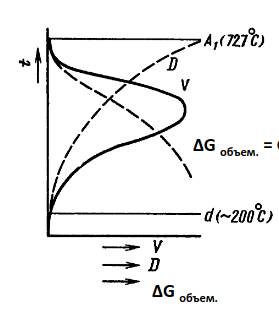
\includegraphics[width=0.6\textwidth]{perlite_speed.png}\caption{Зависимость скорости перлитного превращения (сплошная линия) от температуры}\label{fig:perlite_speed}
\end{figure}
\par Кинетика перлитного превращения описывается уравнение Колмогорова-Аврами (JMAK):
\begin{equation}
y=1-e^{-kt^n}
\label{eq:JMAK}  
\end{equation}
Здесь y - степень превращения, t - время, n - эмпирический параметр.
\begin{figure}[h!]
\centering
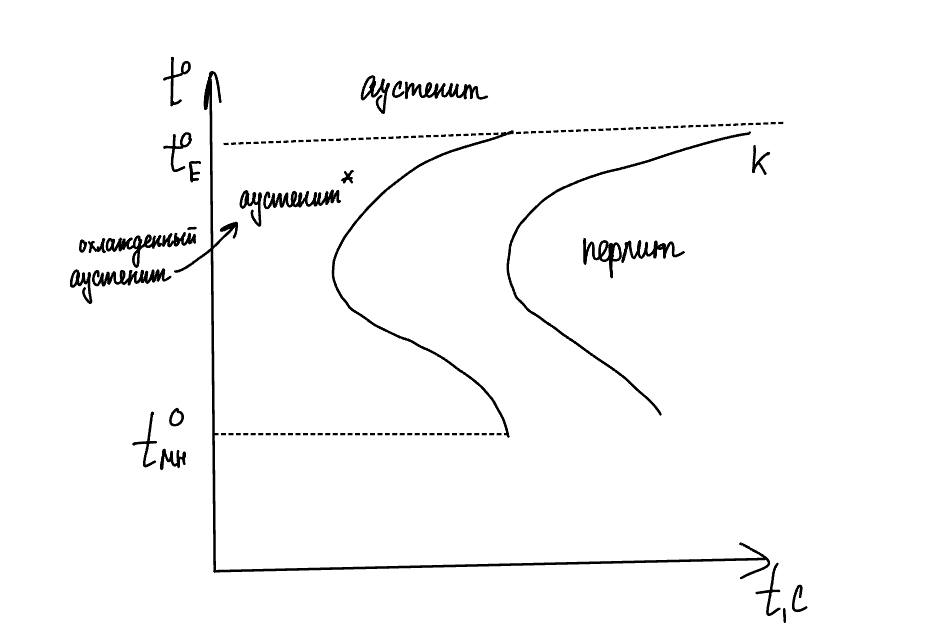
\includegraphics[width=0.4\textwidth]{TTT-diagram.png}\caption{Общий вид ТТТ-диаграммы}\label{fig:TTT-diagram}
\end{figure}
\par Для описания фазовых превращений часто используют изотермические ТТТ-диаграммы (time-transformation-temperature), выглядящие следующим образом (рис. \ref{fig:TTT-diagram}). На рисунке использованы следующие обозначения: н - кривая начала перлитного превращения, к - кривая завершения перлитного превращения, $t_{\text{МП}}^\circ$ - температура начала мартенситного перехода. 
\par На ТТТ-диаграммах удобно выбирать режимы термообработки. Если кривая охлаждения не заходит в перлитную область, то осуществляется закалка на мартенсит. Дифференцировка перлита (перлит, сорбит, троостит - $\lambda \downarrow$) зависит от профиля охлаждения (рис. \ref{fig:cooling_profile}).
\begin{figure}[h!]
\centering
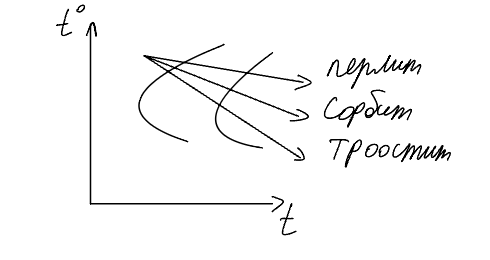
\includegraphics[width=0.4\textwidth]{cooling_profile.png}\caption{Дифференцировка перлита и профиль охлаждения}\label{fig:cooling_profile}
\end{figure}
По ТТТ-диаграммам удобно иллюстрировать различные виды отжига 2-го рода (рис. \ref{fig:annealing2_types}).
\begin{figure}[h!]
\centering
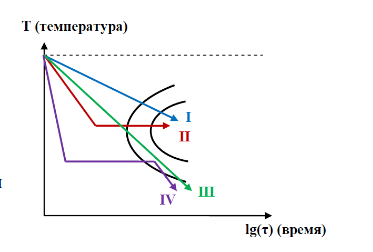
\includegraphics[width=0.4\textwidth]{annealing2_types.png}\caption{Основные виды отжига 2-го рода}\label{fig:annealing2_types}
\end{figure}
На рисунке \ref{fig:annealing2_types} 1 - полный отжиг (медленно, в грубый перлит), 2 - изотермический отжиг (в грубый перлит), 3 - нормализация (в сорбит), 4 - патентирование (в троостит). \par\textit{ИМХО, автор рисунка ошибся с 3 и 4. Кривые следует аккуратно заканчивать в перлитной области, а то это уже не троосит с сорбитом, а бейнит какой-то}

\section{Отжиг 1-го рода. Рекристаллизация. Основные модели процесса спекания.}

\textbf{Отжиг первого (I) рода} --- без фазовой перекристаллизации --- применяется для приведения металла в более равновесное структурное состояние: снимается наклёп, понижается твёрдость, возрастают пластичность и ударная вязкость, снимаются внутренние напряжения (в связи с процессами отдыха и рекристаллизации). \textbf{отжиг первого (I) рода} направлен на возвращение в равновесное состояние металла, подвергнутого предварительной пластической деформации.

\textbf{Виды + характеристика на примере стали}



 \textbf{1. Диффузионный (гомогенизирующий) отжиг.} Применяется для устранения ликвации, выравнивания химического состава сплава. В его основе --- диффузия. В результате нагрева выравнивается состав. Применяется, в основном, для легированных сталей. Полностью снимает внутренние напряжения. Температура гомогенизации должна быть достаточно высокой, однако нельзя допускать пережога, оплавления зерен.

Недостаток: Сопровождается ростом зерна и окалиной. Температура нагрева зависит от температуры плавления, $\text{Т}_\text{н}=0,8* \text{Т}_\text{пл}$, $\mathrm{t}=1100-1200^{\circ} \mathrm{C}$. Продолжительность выдержки: $\tau \approx 8-20$~ч (десятки часов).

\textit{// Это необязательно//} Если допустить пережог, то кислород воздуха окисляет железо, проникая в толщу его, образуются кристаллиты, разобщенные окисными оболочками. Пережог устранить нельзя, поэтому пережженные заготовки являются окончательным браком. Диффузионный отжги стали обычно приводит к слишком сильному укрупнению зерна, что следует исправлять последующим полным отжигом (на мелкое зерно). В стальных слитках в результате диффузионного отжига достигается более равномерное распределение фосфора, углерода и легирующих элементов в объеме зерен твердого раствора. Если температура отжига достаточно высока, отжиг приводит к более благоприятному распределению сульфидов.

\textbf{2. Рекристаллизационный отжиг.} Проводится для снятия напряжений после холодной пластической деформации. Цель: устранение наклепа, созданного холодной пластической деформацией, понижение прочности и восстановление пластичности деформированного металла, получение определенной кристаллографической текстуры, создающей анизотропию свойств, и получение заданного размера зерна. Отжиг первого рода проходит в две стадии: 1) возврат, 2) рекристаллизация.

1) Возврат --- нагрев металла до относительно низких температур. Результат искаженная форма кристаллов сохраняется, снимаются внутренние напряжения в структуре. В результате твердость и прочность незначительно уменьшаются, уменьшается склонность к хрупкому разрушению.

2) Рекристаллизация --- нагрев до высоких температур: \textbf{чистые металлы} --- до $\mathrm{t}_{\mathrm{p}}= 0,2 - 0,3 \cdot \text{Т}_\text{пл}$; \textbf{чистые сплавы} --- до $t_p=0,5-0,6 \cdot \text{Т}_\text{пл}$; \textbf{технические сплавы} --- до $t_p= 0,8-0,9 \cdot \text{Т}_\text{пл}$. Под действием высоких температур происходит полная перестройка кристаллической структуры металла. Вместо деформированных кристаллов в твердом состоянии происходит зарождение и рост новых равновесных кристаллов. Свойства металла возвращаются к исходным --- бывшим до деформации.

\textit{В процессе рекристаллизационного отжига} происходит образование зародышей новых зерен и последующий рост этих зародышей. Постепенно старые деформированные зерна исчезают. Количество дефектов в кристаллической решетке уменьшается, наклеп устраняется, и металл возвращается в исходное состояние.


\textbf{3. Отжиг на полигонизацию} проводят при температуре, которая ниже температуры начала рекристаллизации. Соответственно при такой температуре происходит лишь частичное устранение наклепа за счет процессов возврата второго рода, т.е. происходит уменьшение плотности дефектов кристаллической решетки, образование ячеистой дислокационной структуры без изменения формы зерен. Степень уменьшения наклепа зависит, прежде всего, от температуры. Чем ближе температура к порогу рекристаллизации, тем меньше наклеп, тем больше пластичность и наоборот.


\textbf{4. Отжиг для снятия напряжений} Устранение внутренних напряжений производится с помощью специальных видов отжига. Этот отжиг проводится при температурах ниже температуры рекристаллизации: $\text{Т}_\text{н}= 0,2-0,3 \cdot \text{Т}_\text{пл}$. Повышенная температура облегчает скольжение дислокаций и, под действием внутренних напряжений, происходит их перераспределение, т.е. из мест с повышенным уровнем внутренних напряжений дислокации перемещаются в области с пониженным уровнем. Происходит как бы разрядка внутренних напряжений. При нормальной температуре этот процесс будет длиться в течение нескольких лет. Увеличение температуры резко увеличивает скорость разрядки, и продолжительность такого отжига составляет несколько часов.

\textbf{Спекание}

Спекание --- уплотнение поликристаллических веществ при термообработке (Исключение уменьшение плотности при аномальном росте зерен при рекристаллизации, например керамических и <<литых>> образцов Вi2212 ВТСП при <<спекании>> за счет роста длинных игольчатых кристаллов) Процессы, протекающие при спекании (повышение прочности и плотности):

\begin{itemize}
    \item Уменьшение объема пор,
    \item Увеличение площади контакта между кристаллами
    \item Рост зёрен, изменение их формы и укладки
\end{itemize}

Основной вклад в движущую силу --- уменьшение свободной энергии межфазных границ $\sigma$ (кристалл--газ, жидкость--кристалл, кристалл--кристалл).


\textbf{Основные механизмы}

\textbf{Жидкостное спекание:} плавни, минерализаторы, эвтектики, перитектики (стягивание частиц за счет высокого радиуса кривизны жидкостной прослойки --- перешейка между частицами, быстрый диффузионный перенос компонентов через жидкость, рекристаллизация кристаллитов, изменение реологических свойств во время спекания ползучесть и пр., часто --- понижение температуры спекания)

\textbf{Стадии жидкофазного спекания:}

\begin{enumerate}
    \item Перегруппировка частиц путем взаимного проскальзывания
    \item Перенос материала через жидкую фазу, при этом насыщение жидкой фазы происходит за счет ратворения мелких частич и контактных участков, химический потенциал которых повышен из-за напряжений и пр.
    \item Образование жесткого скелета, залечивание пор
\end{enumerate}

\textbf{Твердофазное спекание} (пластическая деформация частиц (обычно эффективен при приложении внешнего давления), испарение-конденсация - перемещение вещества с поверхности к вогнутой поверхности перешейка между кристаллитами и его «залечивание» - может протекать практически без усадки, диффузионный перенос вещества через перешеек - важно наличие Пространственных и точечных дефектов)

\textbf{Спекание под давлением} (<<горячее прессование>>)

\textbf{Реакционное спекание} (протекание химической реакции и образование новых фаз).

\begin{wrapfigure}{r}{0.2\textwidth}
    \begin{center}
        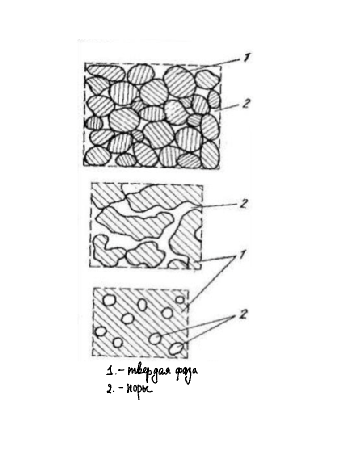
\includegraphics[width=0.2\textwidth]{chem_19_1.png}
    \end{center}
\end{wrapfigure}

\textbf{Ниже представлены основные стадии спекания.}



\textbf{Стадии спекания}


\begin{enumerate}
    \item стадия. \textbf{Припекание}. Создаются и увеличиваются контакты между соседними частицами, но границы зёрен сохраняются. \textit{Движущая сила спекания} --- избыток свободной энергии, связанной с дисперсностью порошка.
    \item стадия. \textbf{Обособление <<фазы вещества>> и <<фазы пустоты>>}. Частицы как бы сливаются, но замкнутых пор ещё не образуется. \textit{Движущая сила спекания} --- избыток энергии свободных поверхностей пор и межзёренных границ.
    \item стадия. Образуются замкнутые поры. \textit{Движущая сила спекания} --- уменьшение протяжённости границы раздела пор кристалла и удаление пор.
    \item студия. Удаления замкнутых пор.
\end{enumerate}


Явления, сопровождающие отжиг 1-го рода:

\begin{enumerate}
    \item Возврат (recovery) --- совокупность процессов самопроизвольного изменения плотности и распределения дефектов (и соответствующих им полей напряжений) в неравновесных (в частности, деформированных) кристаллах до начала рекристаллизации
    \begin{enumerate}
        \item возврат 1-го рода (отдых) --- без миграции малоугловых границ (дислокаций)
        \item возврат 2-го рода (полигонизация) --- миграция малоугловых границ (дислокаций)
    \end{enumerate}
    \item Рекристаллизация --- возникновение новых зерен, рост зерен (grain growth), сопровождающиеся движением высокоугловых границ
    \item Уплотнение (densification) --- уменьшение доли и размера пор
    \item Коалесценция пор (coarsening) --- укрупнение пор без изменения их общего объема
\end{enumerate}

\begin{figure}[h!]
    \centering
    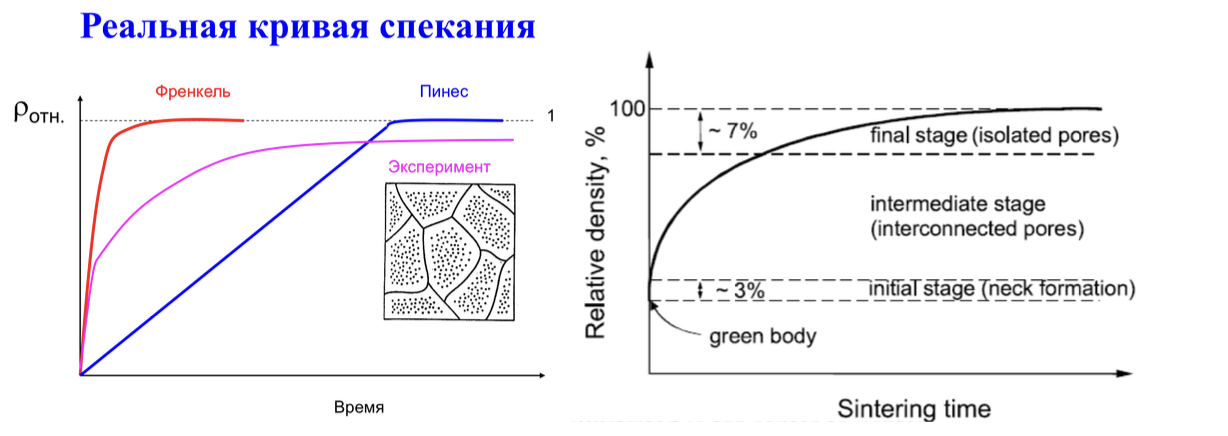
\includegraphics[width=0.8\textwidth]{chem_19_2.png}
\end{figure}


\section{Распад пересыщенного твердого раствора по спинодальному механизму и механизму образования и роста зародышей. Термодинамика процессов распада, роль упругой энергии. Старение материалов естественное и искусственное (на примере дуралюмина).}


\begin{wrapfigure}{r}{0.5\textwidth}
    \begin{center}
        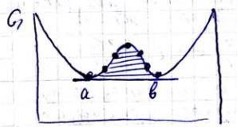
\includegraphics[width=0.4\textwidth]{chem_20_2.jpg}
    \end{center}
\end{wrapfigure}

Термодинамика: фазовая диаграмма и зависимость $G$ от состава. Если в пересыщенном растворе возникает флуктуация состава (в точке К), то в дальнейшем процесс будет происходить самопроизвольно (неустойчивое равновесие в очке К).

\begin{figure}[h!]
    \centering
    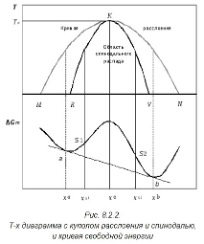
\includegraphics[width=0.4\textwidth]{chem_20_1.jpg}
\end{figure}


Флуктуация состава неравновесна, термодинамически выгоден распад: будет спонтанный постепенный распад на а и b --- \textbf{спинодальный распад} (граница растворимости в твердом состоянии):





\begin{wrapfigure}{r}{0.5\textwidth}
    \begin{center}
        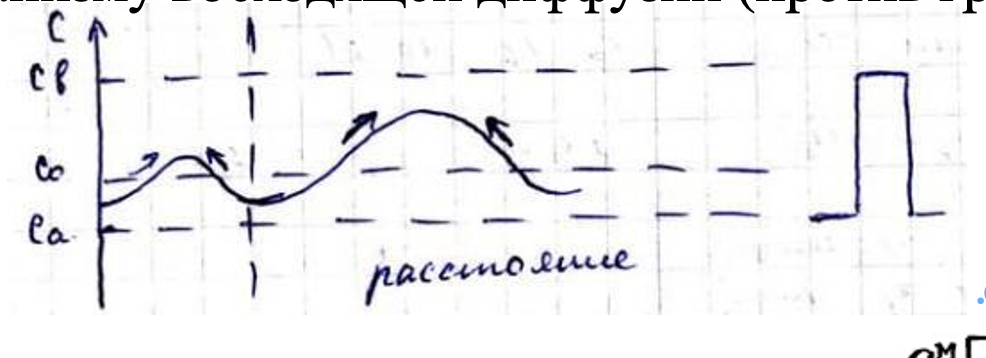
\includegraphics[width=0.4\textwidth]{chem_20_3}
    \end{center}
\end{wrapfigure}

Процесс протекает по механизму восходящей диффузии (против градиента концентраций). Справа --- состав, каким он будет по прошествии бесконечно большого интервала времени.

\textbf{Образование и рост зародышей }

\begin{wrapfigure}{r}{0.4\textwidth}
    \begin{center}
        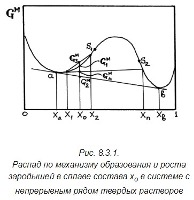
\includegraphics[width=0.4\textwidth]{chem_20_4}
    \end{center}
\end{wrapfigure}

Если происходит распад раствора, отвечающего точке $X_0$, то видно, что малые флуктуации состава термодинамически не выгодны, энергия системы кристаллов выше, чем у исходного раствора (ситуация 1). 

% \begin{wrapfigure}{r}{0.3\textwidth}
%     \begin{center}
%         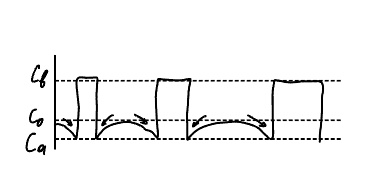
\includegraphics[width=0.4\textwidth]{chem_20_5}
%     \end{center}
% \end{wrapfigure}

\textbf{Для распада} (на $b$ и состав от $a$ до $X_0$) надо преодолеть некий энергетический барьер, необходимо присутствие зародышей новой фазы. Зародыши могут образовываться за счет сегрегации одного из компонентов на дислокациях, границах зерен и других дефектов. Этот процесс не захватывает весь объем, протекает по механизму нисходящей диффузии (по градиенту концентрации).


\pagebreak
\textbf{Сравнение двух процессов}

\begin{table}[h!]
    \centering
    \resizebox{\textwidth}{!}{
    \begin{tabular}{|c|c|}
    \hline
    Спинодальный распад & Образование и рост зародышей \\ \hline
    Флуктуации возникают где угодно & \makecell{Рост зародыша происходит в \\ выделенной зоне (поверхность границы зёрен)} \\ \hline \xrowht{15pt}

    $\frac{\partial ^2 C}{\partial C^2} = 0$ & $0=\frac{\partial G}{\partial C} \leftarrow C\frac{\partial ^2 C}{\partial C^2}$ \\ \hline

    \makecell{$D<0$, против градиента концентрации \\ восходящая дифузия} &  \makecell{$D>0$, по градиенту концентрации \\ нисходящая дифузия} \\ \hline

    Малые флуктуации состава & Зародыш новой фазы\\ \hline

    Состав фазы меняется & $C_a, C_b = const$ \\ \hline
    Размытая граница & Резкая граница \\ \hline

    \makecell{Когерентная граница \\ (сопряжение двух кристаллических решёток)} & $\pm$ \\ \hline

    $\pm$ & \makecell{Наступает термодинамическое \\ равновесие} \\ \hline

    \makecell{Закономерная пространственная \\ ориентация фаз} & $\pm$ \\ \hline
    
\end{tabular}}
\end{table}

\textbf{Термодинамика процессов распада, роль упругой энергии}

\begin{wrapfigure}{r}{0.5\textwidth}
    \begin{center}
        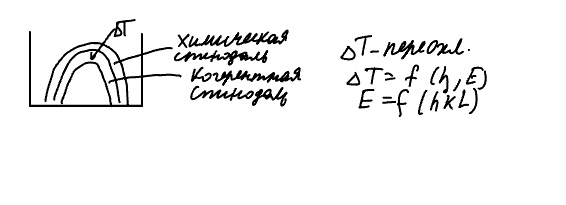
\includegraphics[width=0.5\textwidth]{chem_20_6}
    \end{center}
\end{wrapfigure}

Энергетика процесса спинодального распада определяется вкладом 3х компонент: объемной, поверхностной и упругой: $G= G^\text{об} + G^\text{пов} + G^\text{упр}$. Чем больше удельное изменение параметров решетки, с изменением состава  = $1/a \cdot da dc $ и чем жестче решетка (жесткость решётки определяется E --- модулем Юнга(!)) , тем больше вклад $ G^\text{упр}$. Энергия, выделяющаяся при распаде тратится на деформацию, поскольку изменяются параметры кристаллической решетки. Поэтому в реальности вместо химической спинодали наблюдается когерентная, которая лежит ниже по температуре. 

\textbf{Старение материалов: }
\begin{itemize}
    \item Естественное остаривание: при комнатной температуре, рост выделений внутри зерен.
    \item Искусственное остаривание: при комнатной температуре, рост выделений по границам зерен.  
\end{itemize}


\textbf{На примере дюралюминия (Сплав Cu-Al)}

Только что приготовленный дюралюмин мягкий. При выдерживании его в течение некоторого времени (остаривании) происходит распад твёрдого раствора (спинодальный), при этом возникают мелкие области (20-50~\si{\angstrom} неоднородности), обогащенные медью --- зоны Гинье-Престона (зоны Гинье-Престона --- см. следующий билет) (медь собирается в кластеры --- дискообразные частицы). Медь локализуется в дискообразных кластерах, решетка деформируется. Попадание внутрь купола (см. ниже) --- появление зон Гинье-Престона. Состав неравновесных кластеров может сильно различаться. При остаривании материал упрочняется. Сплав Cu-Al обладает повышенной твердостью и тягучестью (после остаривания).

\textbf{Реальная морфология:}

\begin{figure}[h!]
    \centering
    \includegraphics[width=0.9\textwidth]{chem_20_7}
\end{figure}


\section{Зональная стадия распада твердого раствора; термодинамика и кинетика образования и строение зон Гинье-Престона. Природа упрочнения при дисперсионном старении.}

\textbf{Остаривание} --- (в билете 20) выдерживание материала при невысокой температурах длительное время.

2 основных механизма: 

\begin{enumerate}
    \item \textbf{химический:} при пластической деформации некоторые дислокации проходят через область  зоны, 	поэтому 	будет 	осуществляться пластический сдвиг (дислокация <<перерезает>> зону)
   \includegraphics[width=0.5\textwidth]{chem_21_1}

    \item \textbf{механизм Орована:} образуется скопление частиц --- дислокация подходит к частицам и <<выгибается>>.
    
    \includegraphics[width=0.3\textwidth]{chem_21_2}
\end{enumerate}




При высоких температурах зависимость проходит через максимум. Увеличивается количество частиц, они разрастаются и коалисцируют.

\begin{figure}[h!]
    \centering
    \includegraphics{chem_21_3}
\end{figure}



При высоких температурах механизм Орована вносит незначительный вклад, так как при коалисцировании уменьшается общее число частиц. 


\begin{wrapfigure}{r}{0.4\textwidth}
    \begin{center}
        \includegraphics{chem_21_4}
    \end{center}
\end{wrapfigure}

\textbf{Упрочнение:}
\begin{enumerate}
    \item Выделяющаяся частица имеет больший модуль сдвига, что останавливает дислокации.
    \item Количество выделений (механизм Орована). Дислокации могут остановиться и могут пройти (схема на рисунке).
    \item Зависимость от температуры: сначала прочность растет (выделение мелких частиц), затем снижается (рост включений).
\end{enumerate}

\begin{figure}[h!]
    \centering
    \includegraphics[width=0.6\textwidth]{chem_21_5}
\end{figure}



\section{Принципы химико--термической обработки. Виды термомеханической обработки материалов.}

\textbf{Типичные виды химико--термической обработки}

\begin{enumerate}
    \item цементация (закалка) (насыщение стали углеродом на поверхности). Закалка осуществляется в разной степени в зависимости от содержания углерода.
    \item азотирование (насыщение стали азотом).
    \item цеонирование 	(азотирование и цементация).
    
\end{enumerate}

\textbf{Механизм ХТО}

\begin{enumerate}
    \item выдерживание стальной болванки в соответствующей атмосфере.
    \item Происходит насыщение металла углеродом и (или) азотом --- 
диффузионный процесс.
    \item В результате получаем градиентный материал (состав разный на разном расстоянии от поверхности).  
\end{enumerate}

\textbf{Виды термомеханической обработки (ТМО) материалов}

\begin{enumerate}
    \item ВТМО --- высокотемпературная ($T>T_\text{эвтект}$) --- непосредственно после горячего воздействия давлением (пока аустенитная структура), проводится закалка. Не успевает произойти рекристаллизация.
    \begin{itemize}
        \item \textit{Наклёп} --- упрочнение металлов и сплавов в процессе пластической деформации при температуре ниже температуры рекристаллизации.
        \item \textit{Штамповкой} --- способ изготовления деталей давлением при металлических форм, очертания которых соответствуют очертаниям изготовляемых деталей. 
        \item \textit{Прокаткой} --- обработка давлением путем пропускания его в горячем или в холодном состоянии между вращающимися валками прокатного станка. 
        \item \textit{Рекристаллизация} --- процесс образования и роста (или только роста) одних кристаллических зёрен (кристаллитов) поликристалла за счёт других.
    \end{itemize}
    Наклеп и упрочнение не устраняются и остаются в материале после его остывания.  Чем короче промежуток времени между окончанием всех процессов, когда сталь имеет высокую температуру, тем больше сохранится дислокаций и тем больше будет эффект упрочнения.

    \begin{figure}[h!]
        \centering
        \includegraphics{chem_21_6}
    \end{figure}

    \item НТМО --- низкотемпературная ($T<T_\text{эвтект}$) 
    При низкотемпературной термомеханической обработке металл нагревают до аустенитного состояния, затем охлаждают ниже температуры рекристаллизации, но выше температуры начала мартенситного превращения, то есть температурный интервал пластической деформации составляет примерно 400--600~$\rm ^\circ C$. 
    
\end{enumerate}




Деформация, как и при ВТМО, вызывает наклеп аустенита, рекристаллизации же в этих условиях не происходит. Затем проводится закалка: образуется мартенсит, который, как и в предыдущем способе, наследует дислокации, а значит и упрочнение, полученное при низкотемпературной термомеханической обработке стали. Здесь устранен недостаток первого способа, так как рекристаллизация практически отсутствует и потому наиболее полно используется эффект упрочнения от наклепа.

ТМО позволяет получить достаточно высокую прочность ($\sigma _\text{в}= 2200-3000$~МПа) при хорошей пластичности и вязкости ($\delta= 6 -8\%, \psi = 50-60\%)$. 


\chapter{Физика материалов}

\section{Колебания атомов одномерной двухатомной решетки. Акустические и оптические фононы, температура Дебая. Колебания атомов трехмерной 
решетки (зоны Бриллюэна, законы дисперсии и поверхности постоянной частоты).}

Рассмотрим одномерную решетку Бравэ с двумя ионами в элементарной ячейке, равновесные положения которых есть $na$ и $na+d$. Считаем, что оба иона идентичны, но что $d \leq a/2$, поэтому сила между соседними ионами зависит от того, равно ли это расстояние между ними $d$ или же $a-d$. 

\begin{figure}[h!]
    \includegraphics[width=\textwidth]{phys_1_1.png}
\end{figure}

Предположим, что взаимодействуют ближайшие соседи, причем сила взаимодействия больше для пар с расстоянием $d$, чем для пар с расстоянием $a-d$. Гармоническую потенциальную энергию можно представить в виде:

\begin{equation}
    U^{\text {harm }}=\frac{K}{2} \sum\left[u_1(n a)-u_2(n a)\right]^2+\frac{G}{2} \sum\left[u_2(n a)-u_1([n+1] a)\right]^2
\end{equation}

\noindent где через $u_1(na)$ обозначено смещение иона, совершающего колебания вблизи узла na, а через $u_2(na)$ --- смещение иона, колеблющегося вблизи узла na+d. Положим $K>=G$. Уравнения движения 

\begin{equation}
    \begin{aligned}
    M \ddot{u}_1(n a) & =-\frac{\partial U^{h a r m}}{\partial u_1(n a)}=-K\left[u_1(n a)-u_2(n a)\right]-G\left[u_1(n a)-u_2([n-1] a)\right] \\
    M \ddot{u_2}(n a) & =-\frac{\partial U^{h a r m}}{\partial u_2(n a)}=-K\left[u_2(n a)-u_1(n a)\right]-G\left[u_2(n a)-u_1([n+1] a)\right]
    \end{aligned}
\end{equation}


Ищем решение, представляющее собой волну с частотой $\omega$ и волновым вектором $k$: $u_1(n a)=\varepsilon_1 e^{i(k n a-\omega \mathrm{t})}$ и $u_2(n a)=\varepsilon_2 e^{i(k n a-\omega t)}$. Здесь $\epsilon_1$ и $\epsilon_2$ --- требующие определения постоянные, отношение которых дает относительные амплитуды и фазу колебаний ионов в каждой элементарной ячейке. Как и в моноатомном случае, периодическое граничное условие Борна-Кармана приводит к $N$ неэквивалентным значениям $k$. 

\begin{figure}[h!]
    \begin{center}
        \includegraphics[width=0.7\textwidth]{phys_1_2}
    \end{center}
\end{figure}


\begin{equation}
    k=\frac{1\pi}{a} \frac{n}{N}
\end{equation}

Граничное условие (формулировка для линейной цепочки): соединяем два противоположных конца цепочки с помощью одной такой же <<пружинки>>, как и те, которые соединяют ионы внутри цепочки. 

Из полученных выше выражений получим 

\begin{equation}
    \begin{gathered}
    {\left[M \omega^2-(K+G)\right] \varepsilon_1+\left(K+G e^{-i k a}\right) \varepsilon_2=0} \\
    {\left[M \omega^2-(K+G)\right] \varepsilon_2+\left(K+G e^{i k a}\right) \varepsilon_1=0}
    \end{gathered}
\end{equation}

Данная пара уравнений имеет решение, если обращается в нуль детерминант, составленный из их коэффициентов, т.е. если выполняется условие 

\begin{equation}
    \left[M \omega^2-(K+G)\right]^2=\left|K+G e^{-i k a}\right|^2=K^2+G^2+2 K G \cos k a
\end{equation}

Данные уравнение выполняется для двух положительных значений $\omega$, для которых 

\begin{equation}
    \omega^2=\frac{K+G}{M} \pm \frac{1}{M} \sqrt{K^2+G^2+2 K G \cos k a}
\end{equation}
Причем $\displaystyle \frac{\varepsilon_1}{\varepsilon_2}=\mp \frac{K+G e^{-i k a}}{\left|K+G e^{-i k a}\right|}$

Для каждого из $N$ значений $k$ имеется, таким образом, 2 решения, что дает в целом $2N$ нормальных мод, ка и должно быть при $2N$ степенях свободы (по 2 иона в каждой из N элементарных ячеек). Две кривые зависимости $\omega$ от $k$ носят название 2 ветвей закона дисперсии.

Частота первой ветви $\omega$ пропорциональна $k$ при малых $k$, а на краях зоны Бриллюэна кривая становится почти горизонтальной. Эту ветвь называют акустической, так как ее закон дисперсии при малых $k$ имеет форму $\omega=ck$, характерную для звуковых волн. Вторая ветвь начинается при $k=0$ от значения  $\omega = \sqrt{2(K+G)/M}$ и опускается вниз с ростом $k$, достигая значения $\sqrt{2K/M}$ на границе зоны. Ее называют оптической ветвью, поскольку длинноволновые оптические моды в ионных кристаллах могут взаимодействовать с электромагнитным излучением. 

\textbf{Модель Дебая}

\begin{itemize}
    \item Колебания решетки рассматриваются как фононный газ
    \item Закон дисперсии фононов предполагается изотропным и линейным, то есть $\omega=u_sk$ ($u_s = const$)
    \item Первая зона Бриллюэна, которая представляет собой многогранник в пространстве волновых векторов, заменяется на шар того же объема. Его радиус $q_0$ находится из условия равенства объемов: $V_{\text{з.Бp.}}=\frac{4 \pi q_0^3}{3} \Rightarrow q_0=\left(\frac{6 \pi^2}{V_{\text {яч. }}}\right)^{1 / 3}$
    \item $0<\omega<\omega_{max}=\omega_D$
\end{itemize}

Для сплошной среды число состояний на элемент $dk$: 
\begin{equation}
    \frac{V 4 \pi k^3 d k}{(2 \pi)^3}
\end{equation}

При $\mathrm{T} \gg \Theta_{\mathrm{D}}$, где $\Theta_{\mathrm{D}}=\hbar \omega_{\mathrm{D}}$, температура Дебая, все осцилляторы допускают классическое описание.

$\mathrm{T} \ll \Theta_{\mathrm{D}}$, всегда найдутся осцилляторы, чье движение можно описывать классическими формулами, но остальные требуется описать квантово. 

\section{Спектральная плотность фононов. Модели Эйнштейна и Дебая. 
Теплоемкость кристаллической решетки.}

\textbf{Спектральная плотность колебаний решетки} (фононов) или плотность фононных состояний: $v(\omega)=\frac{1}{V} \frac{d N \omega}{d \omega}$, где $dN_\omega$ --- число фононных мод с частотами, лежащими в интервале ($\omega$; $\omega + d \omega$).

Спектральная плотность удовлетворяет условию нормировки $\displaystyle \int_0^{\infty} v(\omega) d \omega=\frac{3 N}{V_{\text {ячейки }}}$ (здесь $N$
--- число атомов в элементарной ячейке $3D$ кристалла, то есть $3N$ --- число степеней свободы). Зная законы дисперсии фононных ветвей, можно определить плотность фононных состояний как $\displaystyle v(\omega)=\sum_p \int \frac{d^3 \bar{k}}{(2 \pi)^2} \delta\left(\omega-\omega_p(\bar{k})\right)$, где $\delta(\omega)$ --- дельта-функция Дирака. Интеграл взят по первой зоне Бриллюэна. 

\begin{equation}
    \delta(\omega)=\left\{\begin{array}{c}
    +\infty, x=0 \\
    0, x \neq 0
    \end{array}\right.
\end{equation}

\textbf{Модель Эйнштейна}

\begin{itemize}
    \item Атомы в решетке ведут себя как $3N_a$ гармонических осцилляторов, не
    взаимодействуя друг с другом;
    Частота колебаний всех осцилляторов одинакова: $\omega_p(\bar{k})=\omega_E=const$. Модель качественно описывает оптические ветви, для которых $\omega_{\min}<\omega_p(\bar{k})<\omega_{\max}$, причем $\omega_{\min}$ и $\omega_{\max}$ --- величины одного порядка

    Для акустических ветвей модель Эйнштейна в области низких температур неприменима

    \item $\hbar \omega_p(\bar{k}) \geq T$. Так как $\omega_E=const$, $\nu(\omega)=3N\delta(\omega-\omega_E)$
\end{itemize}

\textit{Теплоемкость:}

Вычислим среднюю энергию осциллятора с частотой $\omega_i$ и полную энергию набора осцилляторов, так как фононы подчиняются статистике Бозе-Эйнштейна. 

\begin{equation}
    \bar{\varepsilon}_l=\frac{\hbar \omega_i}{e^{\hbar \omega_i / T}-1} ; \quad E_{\text {полн }}=\sum_{i=1}^{3 N} \frac{\hbar \omega_i}{e^{\hbar \omega_i / T}-1}
\end{equation}

Среднее число заполнения: $\langle n\rangle=\frac{1}{e^{\frac{\hbar \omega_i}{T}}-1}$

\begin{equation}
    E_{\text {полн }}=\int_0^{\omega_{\max }} \frac{\hbar \omega_i}{e^{\frac{\hbar \omega_i}{T}}-1} v(\omega) \mathrm{d} \omega = \int_0^{\omega_{\max }=\omega_E} \frac{\hbar \omega_i * 3 N}{e^{\frac{\hbar \omega_i}{T}}-1} \delta\left(\omega-\omega_E\right) \mathrm{d} \omega= \frac{\hbar \omega_E * 3 N}{e^{\hbar \omega_i / T}-1}
\end{equation}



\begin{equation}
    C_v=\frac{\partial E}{\partial T}=\frac{\hbar \omega_E \cdot 3 N-e^{\frac{\hbar \omega_E}{T}} \cdot \frac{\hbar \omega_E}{T^2}}{\left(e^{\frac{\hbar \omega_E}{T}}-1\right)^2}
\end{equation}


\textbf{Модель Дебая}

\begin{itemize}
    \item Колебания решетки рассматриваются как фононный газ.
    \item Закон дисперсии фононов предполагается изотропным и линейным, то есть $\omega = u_{s}k$, $(u_s=const)$.
    \item Первая зона Бриллюэна, которая представляет собой многогранник в пространстве волновых векторов, заменяется на шар того же объема. Его радиус $q_0$ находится из условия равенства объемов: $V_{\text{з.Бp.}}=\frac{4 \pi q_0^3}{3} \Rightarrow q_0=\left(\frac{6 \pi^2}{V_{\text {яч. }}}\right)^{1 / 3}$
    \item $0<\omega<\omega_{max}=\omega_D$
\end{itemize}

Для сплошной среды число состояний на элемент $dk=\frac{V 4 \pi k^3 d k}{(2 \pi)^3}$. Усредним $\omega=\overline{u_s}k$; $\frac{3}{\overline{u_{s}}^3} = \frac{1}{\overline{u_{e}}^3}+\frac{2}{\overline{u_{t}}^3}$, ($\omega_t=\overline{u_t}k$, $\omega_c=\overline{u_c}$ --- продольные и поперечные волны).
Тогда $\displaystyle \frac{V 4 \pi k^3 d k}{(2 \pi)^3} \rightarrow \frac{V 3 \omega^2 d \omega}{2 \pi^2 \bar{u}_s{ }^3} \rightarrow \nu(\omega)=\left\{\begin{array}{c}\frac{3}{2 \pi^2} \cdot \frac{\omega^2}{\overline{u_s}^3} \omega \leqslant \omega_D \\ 0, \quad \omega>\omega_D\end{array}\right.$

\textit{Теплоёмкость}

\begin{equation}
    C_v=\int_0^{\omega_D} \frac{(-1)  e^{\hbar \omega / T} \cdot \left(\frac{1}{T^2}\right) *(h \omega)^2}{\left(e^{\hbar \omega / T}-1\right)^2} v(\omega) d \omega,
\end{equation}

Новая переменная $\displaystyle \left\{\begin{array}{c}\varkappa=\frac{\hbar \omega}{T} \quad \mid \omega \rightarrow 0 \; \varkappa \rightarrow 0 \\ d \varkappa=\frac{\hbar}{T} d \omega \quad \mid \omega \rightarrow \omega_D \; \varkappa \rightarrow \frac{\Theta_D}{T}\end{array}\left(\Theta_D=\omega_D \hbar\right)\right.$

Тогда 
\begin{equation}
    \begin{aligned} & \left.C_v=\int_0^{\theta_D / T} \frac{e^\chi \chi^2}{\left(e^x-1\right)^2} * \frac{3 T^2 \varkappa^2}{2 \pi^2 \overline{u}_s{ }^2 \hbar^2} * \frac{T}{\hbar} d \varkappa=\frac{3 T^3}{2 \pi^2 \overline{u}^3 \mathrm{\hbar}^3} \int_0^{\theta_D / T} \frac{e^\chi \varkappa^4}{\left(e^x-1\right)^2}=\left( \begin{array}{l} \omega_D=\overline{u}_s k_D \\ \overline{u}_s=b\omega_D / k_D  \end{array}\right. \right) = \\ & =\frac{3}{2 \pi^2} *\left(\frac{T}{\theta_D}\right)^3 k_D{ }^3\left\{\begin{array}{c}T \ll \theta_D \Rightarrow \theta_D / T \rightarrow \infty \Rightarrow \int_0^{\infty} \varkappa^2 d \varkappa=\frac{4 \pi^2}{15} \\ T \gg \theta_D \Rightarrow \int_0^{\theta_D / T} e^{\varkappa} \varkappa^2 d \varkappa \approx \int_0^{\theta_D / T} \varkappa^2 d \varkappa=\frac{1}{3}\left(\frac{\theta_D}{T}\right)^3\end{array}\right. \\ & \end{aligned}
    \end{equation}
    
\begin{equation}
    C_v=\left\{\begin{array}{c}T \ll \theta_D \Rightarrow \frac{3}{2 \pi}\left(\frac{T}{\theta_D}\right)^3 k_D{ }^3 \frac{4}{15} \pi^2=\frac{2 \pi}{5}\left(\frac{T}{\theta_D}\right)^3 k_D{ }^3 \\ T \gg \theta_D \Rightarrow \frac{k_D{ }^3}{2 \pi} \Rightarrow\left\langle\int_0^{\omega_D} v(\omega) d \omega=3 N\right\rangle \Rightarrow \frac{3 N \pi^2}{2 \pi^2}=9 N\end{array}\right. 
\end{equation}


\section{Приближение почти свободных электронов. Поверхности Ферми металлов. Метод Харрисона.}

\begin{figure}[h!]
    \centering
    \includegraphics[width=0.8\textwidth]{phys_1_3.png}
\end{figure}

Применим для металлов; Электроны ведут себя почти как свободные; $U(r)$ мало 
(значительно меньше кинетической энергии); Используются методы теории возмущений 

Рассматривается движение электронов в линейной цепочке прямоугольных потенциальных ям шириной $a$, отделённых барьерами толщиной $b$ и высотой U0. Длина цепочки $L$, период $a+b$.
Решение уравнения Шрёдингера $\frac{\partial^2 \psi}{\partial x^2}+\frac{2 m}{\hbar^2}(E-U) \psi=0$ разбивается на две части

\begin{enumerate}
    \item $\mathrm{U}=0$, волновая функция представляется в виде $\psi_1(x)=A e^{i \alpha x}+B e^{-i \alpha x}$ (первое слагаемое - прямая волна, второе - отраженная от барьера)
    \item $\mathrm{U}=\mathrm{U}_0$, волновая функция: $\psi_2(x)=C e^{\beta x}+B e^{-\beta x}$.
    При этом $\alpha=\sqrt{\frac{2 m e}{\hbar^2}} \quad; \beta=\sqrt{\frac{2 m e\left(U_0-E\right)}{\hbar^2}}$.
\end{enumerate}

Подставляя в одномерную функцию Блоха $\psi(x)=U(x) \exp (i k x)$
$$
U_1(x)=A e^{(\alpha-i k) x}+B e^{-(\alpha+i k) x} ; \quad U_2(x)=C e^{(\beta-i k) x}+B e^{-(\beta+i k) x} .
$$
Oпределим A, B, C, D из непрерывности $U(x)$ и $U^{\prime}(x)$ в местах скачка потенциала. Т.е. для $\mathrm{x}=0$
$$
U_1(0)=U_2(0) ;\left(\frac{\partial U_1}{\partial x}\right)_{x=0}=\left(\frac{\partial U_2}{\partial x}\right)_{x=0}
$$ 

Также воспользуемся периодичностью $U(x): U_1(a)=U_2(-b) ;\left(\frac{\partial U_1}{\partial x}\right)_{x=a}=\left(\frac{\partial U_2}{\partial x}\right)_{x=-b}$

\begin{figure}[h!]
    \centering
    \includegraphics{phys_2_1}
\end{figure}


Подставляя в уравнения для $U_i(x)$, получим
$$
\frac{\beta^2-\alpha^2}{2 \alpha \beta} \mathrm{sh} (\beta b) \sin (\alpha a)+\mathrm{ch}(\beta b) \cos (\alpha a)=\cos k(a+b)
$$

Рассмотрим предельный случай $b \rightarrow 0, U_0 \rightarrow \infty$ при $b U_0= const =\frac{\hbar^2}{m a} P$. $\displaystyle P=\frac{m a}{h^2 b v_0}$ ($\mathrm{P}$ --- прозрачность барьера). Тогда: $\displaystyle P \frac{\sin (\alpha a)}{a d}+\cos (\alpha a)=\cos (k a) \text {. }$

Так как $-1<\cos<1$, левая часть уравнения от -1 до 1. Это и определяет область разрешённых состояний.

Таким образом, при построении зон Бриллюэна в приближении ПСЭ рассматривается чередование запрещенных и разрешенных зон. При этом

\begin{itemize}
    \item на границе $\displaystyle \frac{\partial E}{\partial k} =0$
    
    \includegraphics[width=0.4\textwidth]{phys_2_2} \includegraphics[width=0.2\textwidth]{phys_2_5}
    
    \item размеры зон одинаковы, поэтому число состояний в зонах конечно и одинаково
    \item в расширенной схеме каждая зона повторяется при трансляции на $\bar{a}$ : схема периодична, первая зона --- приведенная зонная схема 
\end{itemize}

\textbf{Заполнение зон Бриллюэна электронами в металлах:}

\begin{enumerate}
    \item Двухкомпонентная квадратичная решётка: 1-я зона --- куб (квадрат), 2-я зона --- призма (4 треугольника)
    \item $E_{\min} ^2 < E_{\max} ^1$ --- металлы Mg, Be (двухзонные). Проводимость: электронная по второй зоне, дырочная по первой (вторая зона заполняется после первой).
\end{enumerate}

\begin{figure}[h!]
    \centering
    \includegraphics[width=0.5\textwidth]{phys_2_3}
\end{figure}



\textbf{Поверхность Ферми} --- поверхность с энергией Ферми, отделяющая пустые состояния от занятых.

\begin{itemize}
    \item Металлы 1-й группы. Na, Li, K, Au, Ag, Cu: первая зона заполнена на половину: $\displaystyle R^2 \pi=\frac{\pi^2}{2 a^2} \Rightarrow R^2=\frac{\pi}{2 a^2} \Rightarrow R=\frac{\pi}{a} \frac{1}{\sqrt{2 \pi}}$, $\displaystyle \mathrm{K}_{\mathrm{F}}=\frac{\pi}{a} \frac{1}{\sqrt{2 \pi}}$
    \item Металлы 2-й группы. Mg, Be, Zn, Cd: $R^2 \pi= \frac{4\pi^2}{a^2} \Rightarrow R^2=\frac{4 \pi}{a^2} \Rightarrow K_F=\frac{2 \sqrt{\pi}}{a}$

\end{itemize}

\begin{figure}[h!]
    \centering
    \includegraphics[width=0.2\textwidth]{phys_2_4}
\end{figure}

\textbf{Метод Харрисона построения поверхностей Ферми металлов}

\begin{figure}[h!]
    \centering
    \includegraphics[width=0.4\textwidth]{phys_2_6}
\end{figure}


\begin{enumerate}
    \item Построение мозаики зон Бриллюэна
    \item Расчёт размеров и построение сфер Ферми с центрами из каждого элемента мозаики
    \item Корректировка границ сфер (пересечение с границами зон под прямым углом)
    \item Классификация полученных объёмов по зонам Бриллюэна (вогнутые поверхности --- к сферам $k+1$-й зоне (дырочные); выпуклые --- электронные в $k$-й зоне)
\end{enumerate}


\section{Предположения и следствия метода сильной связи. Заполнение энергетических зон электронами (металлы, полупроводники и диэлектрики, полуметаллы).}

\begin{figure}[h!]
    \centering
    \includegraphics[width=0.8\textwidth]{phys_1_3.png}
\end{figure}

\textbf{Метод сильной связи:} электрон в твёрдом теле ведёт себя так же, как в изолированном атоме.

\begin{figure}[h!]
    \centering
    \includegraphics{phys_3_1}
\end{figure}

$\displaystyle -n=1,2,3 \ldots\left(H: E=-\frac{R_y}{n^{2}}\right)$ ($E=E(n, \;l)$ в отсутствие полей)

$\displaystyle -l=0,1,2 \ldots \mathrm{n}-1\left(M_{e}=\hbar \sqrt{l(l+1}\right)$

$\displaystyle -m=-l \ldots 0 \ldots l$ ($(2 l+1)$ значений)

$\displaystyle -s= \pm 1(1 / 2)$ (s-подуровень --- вырожден, $p-$ --- трёхкратно вырожден)

Рассмотрим на примере атома натрия.

При переходе от набора изолированных атомов к кристаллу 3s-подуровень оказывается выше барьера. Поэтому движение электронов этого подуровня по всему кристаллу не ограничено. К снижению потенциальных барьеров привело перекрытие волновых функций.

\begin{wrapfigure}{R}{0.4\textwidth}
    \includegraphics[width=0.4\textwidth]{phys_3_2}
\end{wrapfigure}

Уравнение Шрёдингера $\quad\left\{-\frac{\hbar^{2}}{2 m} \nabla^{2}+U(\bar{r})\right\} \psi(\bar{r})=E \psi(\bar{r}) \quad$ для изолированного атома с номером $g$ будет принимать вид $\left\{-\frac{\hbar^{2}}{2 m} \nabla^{2}+U_g(\bar{r})\right\} \psi_{g}\left(\bar{r}-\overrightarrow{R_{g}}\right)=E_{a} \psi_{g}\left(\bar{r}-\overrightarrow{R_{g}}\right)$ ($\overrightarrow{R_{g}}$ --- радиус-вектор узла решётки).

В качестве предполагаемого вида $\psi(\bar{r})$ выберем линейную комбинацию $\sum \limits_{g} a_{g} \psi_{g}$.

Тогда $\psi(\bar{r})=\sum \limits_{g} a_{g} \psi_{g}=\sum \limits_{g} e^{i k \overrightarrow{R_{g}}} \psi_{g}\left(\bar{r}-\overrightarrow{R_{g}}\right)$. При этом около узла $g$ $\psi(\bar{r}) \approx e^{i k \overrightarrow{R_{g}}} \psi_{g}\left(\bar{r}-\overrightarrow{R_{g}}\right)$

$\sum \limits_{g}\left\{\left[-\frac{\hbar^{2}}{2 m} \nabla^{2}+U_g(\bar{r})\right]+\left[U(\bar{r})-U_{g}(\bar{r})\right]-E\right\} e^{i k \overrightarrow{R_{g}}} \psi_{g}=0 \quad$ (вид, $\quad$ чтобы $\quad$ был $\quad$ известный гамельтониан $\Rightarrow \sum \limits_{g}\left\{\left(E_{a}-E\right)+W(\bar{r})\right\} e^{i k \overrightarrow{R_{g}}} \psi_{g}=0$.

$\displaystyle \int \psi_{g}^{*} \psi_{g} d \bar{r}=S\left(R_{g}-R_{g}{ }^{\prime}\right)$ --- интеграл перекрытия


$\displaystyle \int \psi_{g}^{*} w(\bar{r}) \psi_{g} d \bar{r}=A\left(R_{g}-R_{g}{ }^{\prime}\right)$ --- обменный интеграл 

Тогда $\displaystyle \sum \limits_{g} e^{i k \overrightarrow{R_{g}}}\left\{\left(E_{a}-E\right) S\left(\overrightarrow{R_{g}}-\overrightarrow{{R_{g}}^{\prime}}\right)+A\left(\overrightarrow{R_{g}}-\overrightarrow{R_{g}}\right)\right\}=0$.

И, вводя $\bar{q}=\overrightarrow{R_{g}}-\overrightarrow{R_{g}}:\left(E_{a}-E\right) \sum \limits_{g} e^{i k \bar{q}} S(\bar{q})+\sum \limits_{g} A(\bar{q}) e^{i k \bar{q}}=0$,

\noindent где $E$ периодичная по волновому вектору добавка: $E=E_{a}+\frac{\sum \limits_{g} A(\bar{q}) e^{i k \vec{q}}}{\sum \limits_{g} S(\bar{q}) e^{i k \vec{q}}}$.

В суммы входят сначала слагаемые I-го типа (ближайшие соседа, т.е. I сфера), затем вторая сфера и так далее. В числителе учитывается перекрывание волновых функций соседи, в знаменателе для простоты перекрывание не учитывается:

$
\displaystyle
\sum \limits_{g} S(\bar{q}) e^{i k \bar{q}} \int \psi_{g}^{*} \psi_{g} d \bar{r}+\cdots=1$ (остальные слагаемые не учитываются)

$
\displaystyle
\sum_{g} A(\bar{q}) e^{i k \bar{q}} \int \limits _{\bar{q}=0}^{\bar{q}=0} \psi_{g}^{*} w(\bar{r}) \psi_{g} d \bar{r} * 1+A_{1} \sum_{i k} e^{i \bar{k} \bar{q}}$  (второе слагаемое отвечает за соседей из первой координационной сферы)


\begin{figure}[h!]
    \centering
    \includegraphics[width=0.2\textwidth]{phys_3_3}
\end{figure}

Конечное уравнение для $E(\bar{k}) = E_a+\underbrace{C}_{<0}+A_1 \sum e^{i\bar{k} \bar{q}}$.  В простой кубической решётке $E(\bar{k}) = E_a+C+A_1 \left( e^{i k_x a} + e^{-i k_x a} + e^{i k_y a} + e^{-i k_y a} + e^{i k_x a} + e^{-i k_z a}\right) = E_a+C+2A_1 \left( \cos k_x a + \cos k_y a + \cos k_z a\right) $

Следствия МСС:

\begin{enumerate}
    \item При образовании кристаллов из изолированных атомов каждый атомный уровень движется вниз и расширяется $\Rightarrow$ образуются зоны.
    
    \begin{figure}[h!]
        \centering
        \includegraphics[width=0.4\textwidth]{phys_stripes}
    \end{figure}

    \item Каждая зона ограничена $\mathrm{E}_{\min }$ и $\mathrm{E}_{\max .}$
    
    $$
    \begin{aligned}
    & E_{\min }=E_{a}+C-6|A| \quad (\mathrm{C}<0) \\
    & E_{\max }=E_{a}+C+6|A| .
    \end{aligned}
    $$


    Таким образом, ширина зоны $12 \mathrm{~A}_{1}$ $\left(\Delta \mathrm{E}=12\left|\mathrm{~A}_{1}\right|\right)$


    \item  При движении по энергии вверх (при переходе от нижних уровней к верхним) ширина разрещённых зон растёт (внешние оболочки перекрываются сильнее, чем внутренние). При этом ширина запрещенных зон уменьшается.
    \item Разрешённые и запрещенные зоны чередуются, возможно перекрытие зон.
    \item $E(k)$ --- чётная по $k$.
    \item Качественное изменение внешних условий
    
    $\mathrm{T} \uparrow \rightarrow \mathrm{a} \uparrow \rightarrow\left|\mathrm{A}_{1}\right| \downarrow \rightarrow \Delta \mathrm{E} \downarrow \rightarrow \mathrm{E}_{\mathrm{g} \uparrow}$

    $\mathrm{P} \uparrow \rightarrow \mathrm{a} \downarrow \rightarrow\left|\mathrm{A}_{1}\right| \uparrow \rightarrow \Delta \mathrm{E} \uparrow \rightarrow \mathrm{Eg}_{\mathrm{g}} \downarrow$

    \item Вырождение может честично или полностью сниматься при образовании кристалла из атомов.
    \item Заполнение энергетических зон.
\end{enumerate}







C ростом энергии растёт ширина разрешённых зон, а ширина запрещённых зон уменьшается. Из-за высокого положения уровней в какой-то момент возможно перекрывание. При образовании кристаллов вырождение может частично или даже полностью сниматься. Отсюда качественное понимание, как меняются свойства при изменении внешних условий:

$\mathrm{T} \uparrow \rightarrow \mathrm{a} \uparrow \rightarrow\left|\mathrm{A}_{1}\right| \downarrow \rightarrow \Delta \mathrm{E} \downarrow \rightarrow \mathrm{E}_{\mathrm{g} \uparrow}$

$\mathrm{P} \uparrow \rightarrow \mathrm{a} \downarrow \rightarrow\left|\mathrm{A}_{1}\right| \uparrow \rightarrow \Delta \mathrm{E} \uparrow \rightarrow \mathrm{Eg}_{\mathrm{g}} \downarrow$

\textbf{Заполнение энергетических зон: металлы, диаэлектрики, полупроводники}

\begin{table}[h!]
    \centering
    \resizebox{\textwidth}{!}{\begin{tabular}{|c|c|}
        \hline
        N изолированных атомов & Кристалл из N атомов \\
        \hline
        $N * 2(2 l+1)$ & $2 N(2 l+1)$ (число состояний сохраняется) \\
        \hline
        \multicolumn{2}{|c|}{Число уровней сохраняется+сохраняется степень заполнения состояний}  \\
        \hline
        \end{tabular}}
\end{table}

Если в системе из N атомов уровень был заполнен наполовину, то и в кристалле зона будет заполнена наполовину.

Целиком заполненная зона не даёт вклада в проводимость.

\textbf{Классификация твёрдых тел}

\begin{figure}[h!]
    \centering
    \includegraphics[width=0.8\textwidth]{images/phys_3_4.png}
\end{figure}

Полупроводник отличается от диэлектрика только размером запрещённой зоны (у диэлектрика $E_g > 5$эВ, у полупроводника $E_g < 5$эВ).


\section{Волновая функция электрона в кристалле. Теорема Блоха. Квазиимпульс электрона в кристалле. Зоны Бриллюэна.}

Для одного электрона, движущегося в кристалле, уравнение Шрёдингера имеет вид:
$$
\begin{aligned}
& \left\{-\frac{\hbar^{2}}{2 m} \nabla^{2}+U(\bar{r})\right\} \psi(\bar{r})=E \psi(\bar{r}) \\
& U\left(\bar{r}+\bar{a}_{n}\right)=U(\bar{r}), \quad \bar{a}_{n}=n_{1} \bar{a}_{1}+n_{2} \bar{a}_{2}+n_{3} \overline{a_{3}}
\end{aligned}
$$

\noindent U --- потенциал кристаллической решётки, объединяет в себе взаимодействие с решёткой и взаимодействие с другими электронами, $\bar{a_n}$ --- период кристаллической решётки. 

\textbf{Теорема Блоха:} волновая функция электрона в поле периодичного потенциала (в частности в кристалле) может быть предстравлена в виде произведения плоской волны и функции, обладающей той же периодичностью, что и кристаллическая решётка.

$$
\psi_{n k}=e^{i k r} U_{n k}(r), \quad U_{n k}(\bar{r}+\bar{a})=U_{n k}(\bar{r}) \text { --- блоховская функция }
$$

\noindent $\bar{a}$ --- период кристаллической решётки, $n$ --- номер зоны.

$\psi(\bar{r}+\bar{a})=e^{i \bar{k} \bar{a}} \psi(\bar{r})$ --- условие трансляционной симетрии для волновой функции в кристалле.

%$\psi _{\bar{k}} (\bar{r})=e ^{i \bar{k} \bar{a}} U_{\bar{k}} (\bar{r})$ --- будем искать решения уравнения Шрёдингера в виде $\widehat{H} \psi=\varepsilon \psi$

% $
% \begin{aligned}
% & U_{\bar{k}}(\bar{r})=U_{\hat{k}}(\bar{r}+\bar{a}) \text {--- периодичность функции} \\
% & \widehat{H} \psi_{\bar{k}}(\bar{r})=\hat{H} e^{i \bar{k} \bar{r}} U_{k}(\bar{r})=\hat{H} \varepsilon e^{i \bar{k} \bar{r}} U_{k}(\bar{r}) %\\
% & e^{-i \bar{k} \bar{r}} \widehat{H} e^{i \bar{k} \bar{r}} U_{\bar{k}}(\bar{r})=e^{-i \bar{k} \bar{r}} \hat{H} \varepsilon e^{i \bar{k} \bar{r}} U_{k}(\bar{r}) \\
% & \widehat{H}_{k}\left(U_{\bar{k}}(\bar{r})\right)=\varepsilon(\bar{k}) U_{\bar{k}}(\bar{r})\text { (1) (новая задача) }
% \end{aligned}
% $

% Представление волновой функции : 
% $$\psi _{n\bar{k}} = e ^{i\bar{k}\bar{r}} U_{n \bar{k}} (\bar{r}) $$


\textbf{Квазиимпульс в кристалле}


    
% $\hat{\bar{v}}=\frac{\hat{\bar{p}}}{m}=-i \frac{\hbar}{m} \nabla$

Скорость свободного электрона $ \displaystyle \langle\bar{V}\rangle=\int \limits_V A e^{-i \bar{k} \bar{r}}\left(-i \frac{\hbar}{m} \nabla\right) A e^{i \bar{k} \bar{r}} d r =  \frac{-i\hbar}{m}(i k) \underbrace{\int\limits _V A e^{-i \bar{k} \bar{r}} A e^{i \bar{k} \bar{r}} d r}_1 =\frac{\hbar k}{m}=\frac{p}{m}$

p--- импульс.


Скорость электрона в кристалле $\langle \bar{V} \rangle=\int \limits_V \psi^*(\bar{r}) \hat{\bar{V}} \psi(\bar{r}) d \bar{r}$

$\displaystyle \langle\bar{V}\rangle=\int u_k^*(\bar{r}) e^{-i \bar{k} \bar{r}}\left(-i \frac{\hbar}{m} \nabla\right) U_k(\bar{r}) e^{i \bar{k} \bar{r}} d r=  -\left(i \frac{\hbar}{m}\right)(i k) \int u_k^*(r) e^{-i k r} u_k(r) e^{i k r} d r+  \left(-i \frac{\hbar}{m}\right) \int u_k^*(r) e^{-i k r} e^{i k r} \nabla u_k(r) d r= \frac{\hbar k}{m}-i \frac{\hbar}{m} \int u_k^*(r) \nabla u_k(r) d r \neq \frac{p}{m}$

\bigskip

Для описания поведения электрона в кристалле вводится квазиимпульс $P$ такой, что $\displaystyle V=\frac{dE}{dP}$. Вместе с квазиимпульсом вводится квазиволновой вектор $k=P/\hbar$. Далее кразиимпульс будем обозначать $p$.

\textbf{Свойства квазиимульса:}
\begin{enumerate}
    \item $\displaystyle \frac{dp}{dt}=F=\nabla U$, причём $F$ --- внешняя сила.
    \item При отсутствии внешних сил квазиимпульс сохраняется.
    \item Любое искажение периодичности решётки, приводящее к процессам рассеяния электронов на дефектах, можно представить как наложение локальной внешней силы.
    \item Квазиимпульс дискретен ($\Delta p = 2\pi \hbar /a$).
    \item Квазиимпульс изменяется в пределах зоны Бриллюэна (в то время как импульс свободного электрона может принимать значения $[0; +\infty)$)
\end{enumerate}

Возьмём большой кристалл ($L \gg a$). Внутреннюю область разбиваем на блоки размером $L_x$, $L_y$, $L_z$.
$\psi(x; y; z) = \psi(x +L_x; y; z) = \psi(x; y+L_y; z) = \psi(x; y; z+L_z)$

$\psi(x+L_x)=\psi(x) \Rightarrow U_{k}(x+L_x)e^{ik_{x} (x+L_x)}=U_k(x)e^{ik_{x} x}$

Так как $e^{ik_{x} L_x}=1$, то $k_x L_x=2 \pi n$ ($n$ --- целое). Из этого следует дискретность квазиволнового вектора, так как $p=\hbar k$, то и дискретность квазиимпульса.

\textbf{Зона Бриллюэна} --- отображение ячейки Вигнера-Зейтса в обратном пространстве. В приближении Блоха волновая функция электрона для периодического потенциала решетки полность описывается ее поведением в 1 зоне Бриллюэна. 1я зона Бриллюэна содержит точку $k=0$ (2я зона непосредственно прилегает к 1 и так далее); она может быть построена как объем, ограниченный плоскостями, которые отстоят на равные расстояния от рассматриваемого узла обратной решетки до соседних узлов. Для простой кубической решетки зона Бриллюэна --- кубооктаэдр (14-граник).

\begin{figure}[h!]
    \centering
    \includegraphics[width=0.8\textwidth]{phys_4_1.png}
\end{figure}

Число разрешённых (возможных) состояний квазиволнового вектора в зон Бриллюэна конечно. Число разрешённых состояний в кристалле с параметром решётки $a$ и периодичностью квазиволнового вектора $2\pi /L$: $\frac{2\pi}{a} / \frac{2\pi}{L} = 2 L/a = 2N$. $N$ --- количество атомов в атомной решётке, 2 из-за возможных ориентаций спина.

Все зоны Бриллюэна имеют одинаковый объём.



\section{Закон дисперсии, изоэнергетическая поверхность, эффективная масса электрона в кристалле}

\textbf{Закон дисперсии} --- зависимость энергии от квазиимпульса в разрешенной зоне ($E(p)$).

\textit{Классификация:}

\begin{enumerate}
    \item Квадратичные ($E \sim p^2$)
    \begin{enumerate}
        \item Квадратичный изотропный $E=\frac{p^2}{2 m^*}$ (изоэнергетическая поверхность --- сфера, $R=\sqrt{2m^*E}$)
        \item Квадратичный анизотропный $E=\frac{p_x^2}{2 m_x}+\frac{p_y^2}{2 m_y}+\frac{p_z^2}{2 m_z}$ (изоэнергетическая поверхность --- трёхосный эллипсоид. Для случая $m_x=m_y$ --- эллипсоид вращения).
    \end{enumerate}
    \item Неквадратичные ($E \nsim p^2$, $m^* \neq const \quad m^* \uparrow \uparrow E$)
    \begin{enumerate}
        \item Закон Кейна (изотропный) $E(1+\frac{E}{E_g})=\frac{p^2}{2m^*}$ (изоэнергетическая поверхность в близи экстремума --- сфера $R=\sqrt{2m^*(0)E(1+E/E_g)}$)
        \item Закон дисперсии в методе сильной связи (для ПКР) $E=E_a+C+2 A_1\left(\cos \left(k_x a\right)+\cos \left(k_y a\right)+\cos \left(k_z a\right)\right)$ (В окрестностях экстремумов выраждается в квадратичный закон $E=|A_1|a^2k^2$, изоэнергетическая поверхность в близи экстремума --- сфера $R=\sqrt{E/(|A_1|a^2)}$)
    \end{enumerate}
\end{enumerate}

\textbf{Эффективная масса электрона}

Введение эффективной массы электрона позволяет описывать его движение в кристалле при помощи законов механики. $\displaystyle \frac{1}{m^*} = \frac{d^2E}{dp^2}$. В близи минимума энергии $m^*>0$, в близи максимума энергии $m^*<0$. 

В трёхмерном случае $m^*$ --- тензор, который можно диагонализировать правильным выбором точки отсчёта.


$$
    \widetilde{m^*}^{-1}=\left(\begin{array}{ccc}
    \frac{\partial^2 E}{\partial p_x^2} & \frac{\partial^2 E}{\partial p_x \partial p_y} & \frac{\partial^2 E}{\partial p_x \partial p_z} \\
    \frac{\partial^2 E}{\partial p_y \partial p_x} & \frac{\partial^2 E}{\partial p_y^2} & \frac{\partial^2 E}{\partial p_y \partial p_z} \\
    \frac{\partial^2 E}{\partial p_z \partial p_x} & \frac{\partial^2 E}{\partial p_z \partial p_y} & \frac{\partial^2 E}{\partial p_z^2}
    \end{array}\right) \rightarrow \left(\begin{array}{ccc} m_1^{-1} & 0 & 0 \\ 0 & m_2^{-1} & 0 \\ 0 & 0 & m_3^{-1} \end{array}\right)
$$

$\bar{F}_\text{внеш} =  \widetilde{m^*}\bar{a}$

\section{$\rm k \cdot p$--метод. Энергетический спектр электрона в однозонном приближении. Правила сумм. Взаимодействие энергетических зон}

\textbf{$\rm k \cdot p$--метод.}

Методы расчёта <<из первых принципов>> не обладают достаточной точностью для расчёта энергетических зон узкощелевых полупроводников так как:

\begin{enumerate}
    \item $E_g$ в данных материалах может быть <0,1эВ (или 0эВ)
    \item Результат получается в численном виде (таблица с числами в пределах зоны Бриллюэна). В УЩПП необходимо знать закон дисперсии в окрестности экстремумов зон ($E_c (k)$ и $E_v (k)$) в аналитическом виде.
\end{enumerate}

Преимущество $\rm k \cdot p$--метода --- при расчёте используются экспериментальные данные, а в результате получается аналитический вид закона дисперсии.

\textbf{Предположения:}

\begin{itemize}
    \item $\psi _{n k_0}(\bar{r})$ --- волновые функции в экстремумах зон
    \item $E_n(\bar{k_0})$ --- энергия краёв зон
    \item Матричные элементы оператора импульса (из эксперимента)
\end{itemize}
 То есть известны решения уравнения Шрёдингера $\displaystyle \left\{\frac{\widehat{\bar{p}^2}}{2 m}+U(\bar{r})\right\} \psi_{n k_0}(\bar{r})=E_n\left(\bar{k}_0\right) \psi_{n k_0}(\bar{r})$. Можно найти $\displaystyle \left\{\frac{\widehat{\bar{p}^2}}{2 m}+U(\bar{r})\right\} \psi_{n k_0}(\bar{r})=E_n\left(\bar{k}_0\right) \psi_{n k}(\bar{r})$ в малых окрестностях экстремумов зон $k_0$. То есть можно найти законы дисперсии.

 \begin{figure}[h!]
    \centering
    \includegraphics[width=0.2\textwidth]{phys_7_1}
    
 \end{figure}

 \begin{enumerate}
    \item Переход от уравнения для $\psi_{nk}$ к уравнению $U_{nk}$. 
    
    $\psi_{n k}(\bar{r})=U_{n k}(\bar{r}) e^{i \bar{k} \bar{r}}$ 
    
    $\displaystyle \psi_{n k}(\bar{r})=U_{n k}(r) e^{i \bar{k} \bar{r}} \hat{\bar{p}}\left(U_{n k} e^{i \bar{k} \bar{r}}\right)=e^{i \bar{k} \bar{r}} \hat{\bar{p}} \left( U_{n k} \right) + U_{n k} \hat{\bar{p}} \left( e^{i \bar{k} \bar{r}} \right) =e^{i \bar{k} \bar{r}} \hat{\bar{p}} \left( U_{n k} \right)+ \hbar k  e^{i \bar{k} \bar{r}}U_{n k}= e^{i \bar{k} \bar{r}}(\hat{\bar{p}}+\hbar \bar{k}) U_{n k}$
    
    $\hat{\bar{p}} \left( \hat{\bar{p}}\left(u_{n k} e^{i \bar{k} \bar{r}}\right) \right) =\ldots=e^{i \bar{k} \bar{r}}(\hat{\bar{p}}+ \hbar \bar{k})^2 U_{n k}$
    
    $\displaystyle \underbrace{\left\{\frac{(\hat{\bar{p}}+\hbar k)^2}{2 m}+U(\bar{r})\right\}}_{\hat{H}_k} U_{nk}(\bar{r}) =E_n(\bar{k}) U_{n k}(\bar{r})$


    $\hat{\bar{p}} \overset{\psi_{nk} \rightarrow U_{nk}}{\longrightarrow} (\hat{p}+\hbar k)$

    $\left\{\frac{(\hat{\hat{p}}+\hbar k)^2}{2 m}+U(\bar{r})\right\}=\hat{\mu}_k$

    \item Выделение оператора $\hat{H}_{k_0}$ и дополнительного возмущения зависящего от $(k-k_0)$
    
    $\displaystyle \hat{H}_k=\frac{\hat{\bar{p}}^2}{2 m}+\frac{\hbar}{m} \bar{k}\bar{p}+\frac{\hbar^2 k^2}{2 m} +U(\bar{r})$
    
    $\displaystyle \hat{H}_k=\hat{H}_{k_0}+\hat{V}$
    
    $\displaystyle \hat{H}_k=\hat{H}_{k_0}+\frac{\hbar}{m}\left(\bar{k}-\hat{k}_0\right) \hat{\bar{p}}+\frac{\hbar^2}{2 m}\left(\bar{k}-\bar{k}_0\right)$
    
    $\displaystyle \hat{V}=\frac{\hbar}{m}\left(\bar{k}-\bar{k}_0\right) \hat{\bar{p}}+\frac{\hbar^2}{2}\left(\bar{k}-\bar{k}_0\right) $

    $\hat{V}$ --- возмущение.

    $\displaystyle \hat{V}$ возрастает при удалении $\bar{k}$  от $\bar{k}_0$.

    \item Применяем теорию возмущений. Разложение $U_{nk}(\bar{r})$ в ряд по известным $U_{nk_0}(\bar{r})$. Подставляем в уравнение, умножаем на $U^*_{nk_0}$, интегрируем по элементарной ячейке. Переходим к системе уравнений относительно $C_{nn^\prime}$
    
    $\sum_{n^{\prime}} C_{n n^{\prime}}\left[\int U_{n k_0}^* \hat{H}_{k_0} U_{n^{\prime} k_0} d \bar{r}\right. +\frac{\hbar}{m}\left(\bar{k}-\bar{k}_0\right) \int U_{n k_0}^* \hat{\bar{p}} U_{n^{\prime} k_0} d \bar{r}^*\left.+\frac{\hbar^2}{2 m}\left(\bar{k^2}- \bar{k^2}_0\right) \int U_{n k_0}^* U_{n^{\prime} k_0} d r\right]= \sum_{n^{\prime}} C_{n n^{\prime}} E_n(\bar{k}) \underbrace{\int U_{n k_0}^* U_{n^{\prime} k_0} d r}_{\delta_{n n_1}}$

    $\int U_{n k_0}^* \hat{H}_{k_0} U_{n^{\prime} k_0} d \bar{r} = E_n (\bar{k}_0)\delta_{nn^\prime}$
    
    $\left\langle U_{n k_0}|\hat{\bar{p}}| U_{n^{\prime} k_0}\right\rangle=p_{n n^{\prime}}\left(\bar{k}_0\right)$ --- матричный оператор импульса.

    \item Определитель системы должен быть равен <<0>>
    
    $\mathrm{det} \Bigg| \left[\left\{E_1(\bar{k}_0)-E_n(\bar{k})+\frac{\hbar^2}{2 m} \right\} \delta_{n n^{\prime}}+\frac{\hbar}{m}(\bar{k}-\bar{k}_0) p_{n n^{\prime}}(\bar{k}_0)\right]  \Bigg| =0$

    В общем случае $n=\infty$

 \end{enumerate}

Решая определитель можно получить законы дисперсии для $E_n(\bar{k})$. Мешает то, что надо знать много значений оператора импульса и наличие большого количества зон.

\textbf{Однозонное приближение}

1 зона с номером $n$. В идём в конец 3 пункта, $n=n^\prime$. $E(\bar{k}_0) - E(\bar{k}) + \frac{\hbar}{2m}(\bar{k}^2 - \bar{k}^{2}_0) + \frac{\hbar}{m}(\bar{k} - \bar{k}_0)\bar{p}_{nn}(\bar{k}_0)=0$

Воспользовавшись $p_{A n}(k_0)=-\hbar k_0$ получаем $E(\bar{k})=E\left(\bar{k}_0\right)+\frac{\hbar^2\left(\bar{k}-\bar{k}_0\right)^2}{2 m}$.

\textbf{Правила сумм}

Вернёмся в конец пункта 2.

$\mathrm{H}=\hat{H}_{k_0}+\frac{\hbar}{m}\left(\bar{k}-\bar{k}_0\right) \hat{\bar{p}}+\frac{\hbar^2}{2 m}\left(\bar{k}^2-\bar{k}_0^2\right)$

В теории возмущений для невырожденных состояний 

$\left(\hat{H_0}+\hat{U}\right) \psi=E \psi \quad E=E_0+E_1+E_2+\ldots$

$E_1=V_{n n}=\int \psi_n^* \hat{V} \psi_n d r$

$E_L=\sum_{n^{\prime} \neq n} \frac{V_{n n^{\prime}} \cdot V_{n^{\prime} n}}{E_n(0)-E_{n^{\prime}}(0)}$

$E_n(\bar{k})=E_n\left(\bar{k}_0\right)+\underbrace{\frac{\hbar}{m}\left(\bar{k}-\bar{k}_0\right) \int U_n^* \hat{М} U_n d r+\frac{\hbar^2}{2 m}\left(k^*-k_0^2\right) \int U^* U d r}_{E_1} + \underbrace{\frac{\hbar^2}{m^2} \sum_{n^{\prime} \neq n} \frac{\left(k-k_0\right) p_{n n^{\prime}}\left(\bar{k}_0\right) \cdot\left(k-k_0\right) p_{n^{\prime} n}\left(\bar{k}_0\right)}{\left(E_n \bar{k}_0\right)-E_{n^{\prime}}\left(\bar{k}_0\right)}}_{E_2} + E_3+ \ldots$

$\hbar (\bar{k}-\bar{k}_0)=\bar{p}$ --- квазиимпульс.

$E=E_n\left(E_0\right)+\frac{p^2}{2 m^*}$

$\displaystyle 
\left.\begin{array}{l}\frac{1}{m^*}=\frac{1}{m}+\frac{2}{m^2} \sum \frac{p_{n n}\left(\bar{k}_0\right) p_{n^\prime n}\left(k_0\right)}{E_n\left(k_0\right)-E_{n^{\prime}}\left(k_0\right)}+\ldots \\ E_n(\bar{k})=E_n\left(\bar{k}_0\right)+\frac{p^2}{2 m}+\frac{1}{m^2} \sum_{n^\prime \neq n} \frac{\bar{p} \bar{p}_{n^\prime n}\left(k_0\right) \cdot \bar{p} \bar{p}_{n^\prime n }\left(k_0\right)}{E_n\left(k_0\right)-E_{n^\prime}\left(k_0\right)}+\ldots\end{array}\right\} \text{--- правила сумм}$

\textit{Правила сумм} для $E_n(\bar{k})$ и $m^*$:

\begin{enumerate}
    \item Отклонение сумм для $E_n(\bar{k})$ от квадратичного изотропного закона и $m^*$ от $m$ --- следствие учёта наличия других зон.
    \item Вклад других зон --- знакопеременный.
    \item Количественно ряд зависит от $E_n-E_{n^\prime}$ и от величины $p_{nn^\prime}(\bar{k}_0)$.
\end{enumerate}

Если $p_{nn^\prime}(\bar{k}_0)=0$, то зоны не взаимодействуют. Если $p_{nn^\prime}(\bar{k}_0)\neq 0$, то говорят, что зоны взаимодествуют.


\section{Параметры зонной структуры полупроводников. Зонная структура основных полупроводниковых материалов.}

\textbf{Основные параметры зонной структуры:}

\begin{enumerate}
    \item Кристаллическая решётка
    \item Форма зоны Бриллюэна и расположение в ней основных точек симметрии и направлений
    \item Положение экстремумов зон в зоне Бриллюэна, величина $E_g$.
    \item Законы дисперсии и изоэнергетические поверхности в окрестностях экстремумов зон.
\end{enumerate}

\textit{//для справки//}

Для ГЦК решётки 1 зона Бриллюэна --- кубооктаэдр в ней

$\Gamma$ --- центр зоны Бриллюэна

$X$ --- центры квадратных граней (3 штуки)

$L$ --- центры гексогональных граней (4 штуки)

$\Sigma$ --- внутри зоны Бриллюэна в направлении типа $\langle 110 \rangle$ (12 штук)

$\Delta$ --- внутри зоны Бриллюэна в направлении типа $\langle 100 \rangle$ (6 штук)



\textbf{Зонная структура Ge и Si}

\begin{enumerate}
    \item Кристаллическая решётка типа алмаза (2 ГЦК подрешётки, сдвинутые друг относительно друга на $\frac{1}{4}$ пространственной диагонали куба)
    \item Зона Бриллюэна такая же как и у ГЦК решётки Браве --- 14-гранник
    \item Ge: минимум зоны проводимости в точках $L$ (4 точки на зону Бриллюэна). максимум валентной зоны в точке $\Gamma$ (1 точка)
    
    $E_g \approx 0,67$~эВ при $T=300$~К

    Si: минимум зоны проводимости в точках $\Delta$ (6 штук на зону Бриллюэна), максимум валентной зоны в точке $\Gamma$ (1 точка)
    
    $E_g \approx 1,1$~эВ при $T=300$~К

    \begin{figure}[h!]
        \centering
        \includegraphics[width=0.5\textwidth]{phys_8_1}
    \end{figure}

    \item Зона проводимости: $\displaystyle E(\bar{k}) = \frac{\hbar^2 k_\perp ^2}{2m_t^*} + \frac{\hbar^2 k_\parallel ^2}{2m_l^*}$
    
    $k_\perp ^2 = k_x ^2 + k_y ^2$, $k^2_\parallel = k^2 _z$

    Ge: $k_\parallel \parallel \langle 111 \rangle$

    Si: $k_\parallel \parallel \langle 100 \rangle$

    Изоэнергетические поверхности --- эллипсоиды вращения.

    \item Валентная зона: $\displaystyle E_{1;2}=-\frac{\hbar^2}{2m}\left[ Ak^2 \pm \left( B^2k^4 + c^2(k_x^2k_y^2+ k_y^2k_z^2 + k_x^2k_x^2) \right)^0,5 \right]$, (A, B, C --- безразмерные константы). Изоэнергетические поверхности --- гофрированные сферы.
    
    $E_3 (\bar{k})=-\frac{\hbar^2 \bar{k}^2}{2m^*_3}$, $m^*_3=\frac{m}{A}$. Изоэнергетические поверхности --- сферы.
\end{enumerate}





\textbf{Зонная структура $A^3B^5$}

A: In, Ga, Al...

B: Sb, As, P, N...

Общая (наиболее распространённа)я ситуация

\begin{enumerate}
    \item Кристаллическая решётка типа сфалерита (цинковой обманки)
    \item Зона Бриллюэна --- кубооктаэдр
    \item Закон дисперсии Кейна
\end{enumerate}

\begin{figure}[h!]
    \centering
    \includegraphics[width=0.4\textwidth]{phys_8_2}
\end{figure}

Отклонение от этой системы:

\begin{itemize}
    \item GaN, InN, AlN кристаллизуются в решётки вюрцита (ГПУ)
    \item Наличие у ряда полупроводников дополнительных экстремумов в зоне проводимости
\end{itemize}

\begin{figure}[h!]
    \centering
    \includegraphics[width=0.8\textwidth]{phys_8_3}
\end{figure}

\begin{figure}[h!]
    \centering
    \includegraphics[width=0.7\textwidth]{phys_8_4}
\end{figure}

Прямозонные используются в оптике.


\textbf{Зонная структура $A^2B^6$}

A: Zn, Cd, Hg...

B: O, Se, S, Te...

\begin{enumerate}
    \item Кристаллическая решётка типа сфалерита или вюрцита
    \item Зона Бриллюэна --- кубооктаэдр
    \item Выполняется закон Кейна
\end{enumerate}

Особенности полупроводников на основе Hg:

\begin{enumerate}
    \item При низких температурах существуют свободные носители заряда (как в металлах)
    \item Инверсная зонная структура ($E_g<0$ в законе Кейна)
\end{enumerate}

\begin{figure}[h!]
    \centering
    \subfigure{
    \includegraphics[width=0.4\textwidth]{phys_8_5}}
    \subfigure{
    \includegraphics[width=0.5\textwidth]{phys_8_6}}
\end{figure}


\textbf{Зонная структура $A^4B^6$}

A: Sn, Ge, Pb...

B: O, S, Se, Te...

\textit{Кристаллическая структура}

\begin{enumerate}
    \item Кубические модификации (решётки типа NaCl). Зона Бриллюэна --- кубооктаэдр
    \item Ромбическая решётка (деформация куба вдоль $\langle 111 \rangle$) (CdTe)
    \item Орторомбическая (деформация куба вдоль $\langle 110 \rangle$) (PbTe)
\end{enumerate}


\vspace{2cm}

\begin{figure}[h!]
    \centering
    %
    \subfigure{
        \includegraphics[width=0.2\textwidth]{phys_8_7}}
    \subfigure{
    \includegraphics[width=0.2\textwidth]{phys_8_8}}
\end{figure}



\vfill

\textbf{Модель инверсии зон Диммака}

\begin{figure}[h!]
    \centering
    \subfigure{
    \includegraphics[width=0.45\textwidth]{phys_8_9}}
    \subfigure{\includegraphics[width=0.45\textwidth]{phys_8_9.2}}

\end{figure}

\begin{figure}[h!]
    \centering\subfigure{
    \includegraphics[width=0.45\textwidth]{phys_8_10}}
    \subfigure{
    \includegraphics[width=0.45\textwidth]{phys_8_11}}
\end{figure}

Справа от весщелевого состояния $E_g \downarrow \uparrow T$, слева от бесщелевого сотояния $E_g \uparrow \uparrow T$.

Для полупроводников на основе свинца наблюдается рост с насыщением запрещённой зоны от температуры (для большинства других полупроводников с ростом температуры запрещённая зона уменьшается). С ростом температуры края зон $L{6}$ и $L_{\bar{6}}$ расходятся (увеличение запрещённой зоны), а край зоны $\Sigma$ движется вверх (приблизительно с такой же скорость, что и $L_6$). С некоторого момента зона $\Sigma$ оказывается выше $L{6}$ (выход на насыщение).

До точки $x\leq 0,3$ можно использовать модифицированный закон Кейна ($\displaystyle E\left(1+\frac{E}{E_g}\right)=\frac{\hbar^2 k_\perp^2}{2 m_t^*(0)}+\frac{\hbar^2 k_\parallel^2}{2 m_l^*(0)}$, 2 параметра $m_t$ и $m_l$).

Далее лучше закон дисперсии Диммака ($\left(\frac{E_g}{2}+\frac{p_\perp^2}{2 m_t^{-}}+\frac{p_\parallel^2}{2 m_t^{-}}-E\right)\left(-\frac{E_g}{2}-\frac{p_\perp^2}{2 m_t^{+}}-\frac{p_\parallel^2}{2 m_t ^+}-E\right)=E_\perp \frac{p_\perp^2}{2 m}+E_\parallel \frac{p_\parallel^2}{2 m}$, $m_t^{ \pm}$, $m_l^{ \pm}$, $E_\perp$, $E_\parallel$ ---  6 параметров, определяются только экспериментально).


\begin{figure}[h!]
    \centering
    \includegraphics[width=0.6\textwidth]{phys_8_12}
\end{figure}

\section{Прямой и инверсный спектры Кейна для полупроводников $A^3B^5$ и $A^2B^6$.}

\textbf{Зонная структура $A^3B^5$}

A: In, Ga, Al...

B: Sb, As, P, N...

Общая (наиболее распространённа)я ситуация

\begin{enumerate}
    \item Кристаллическая решётка типа сфалерита (цинковой обманки)
    \item Зона Бриллюэна --- кубооктаэдр
    \item Закон дисперсии Кейна:

    $$\left\{ \begin{array}{c}
        E_c=E_g+\frac{1}{2} E_g \left( \sqrt{1+\frac{8k^2P^2}{3E_g^2}} -1  \right) \\
        E_{v_1} = -\frac{\hbar^2 k^2}{2m}\\
        E_{v_2} = -\frac{E_g}{2}\left( \sqrt{1+\frac{8k^2P^2}{3E_g}} -1 \right)\\
        E_{v_3} = -\Delta - \frac{P^2k^2}{3(E_g+\Delta)}
    \end{array} \right.$$
    
    $\Delta$ --- энергия спинорбитального взаимодествия, $P=\frac{\hbar}{m} \int U^*_c \hat{\bar{p}} U_{v_2} d\bar{r}$ --- матричный элемент оператора импульса ($\hat{\bar{p}}=-i\hbar \nabla$), $U_c$, $U_{v_2}$ --- блоховские амплитуды.
    
    Неквадратичный закон для электронов и лёгких дырок (зоны проводимости и лёгких дырок зеркальны ($m_c^*=m_{v_2}^*$)).
    
    При выборе начала отсчёта на уровне Ферми закон превращается в $E\left(1+\frac{E}{E_g}\right)=\frac{2 k^2 p^2}{3 E_g} \leftrightarrow \frac{\hbar^2 k^2}{2 m^*}$. В узкощелевых полупроводниках необходимо учитывать вклад $1+\frac{E}{E_g}$, эффективная циклотронная масса  $m^*_c(E)=m^*(0)(1+\frac{2E}{E_g})$.
\end{enumerate}

\begin{figure}[h!]
    \centering
    \includegraphics[width=0.4\textwidth]{phys_8_2}
\end{figure}

Отклонение от этой системы:

\begin{itemize}
    \item GaN, InN, AlN кристаллизуются в решётки вюрцита (ГПУ)
    \item Наличие у ряда полупроводников дополнительных экстремумов в зоне проводимости
\end{itemize}

\begin{figure}[h!]
    \centering
    \includegraphics[width=0.8\textwidth]{phys_8_3}
\end{figure}

\begin{figure}[h!]
    \centering
    \includegraphics[width=0.7\textwidth]{phys_8_4}
\end{figure}

Прямозонные используются в оптике.


\textbf{Зонная структура $A^2B^6$}

A: Zn, Cd, Hg...

B: O, Se, S, Te...

\begin{enumerate}
    \item Кристаллическая решётка типа сфалерита или вюрцита
    \item Зона Бриллюэна --- кубооктаэдр
    \item Выполняется закон Кейна
\end{enumerate}

Особенности полупроводников на основе Hg:

\begin{enumerate}
    \item При низких температурах существуют свободные носители заряда (как в металлах)
    \item Инверсная зонная структура ($E_g<0$ в законе Кейна)
\end{enumerate}

\begin{figure}[h!]
    \centering
    \subfigure{
    \includegraphics[width=0.4\textwidth]{phys_8_5}}
    \subfigure{
    \includegraphics[width=0.5\textwidth]{phys_8_6}}
\end{figure}


$\displaystyle E=\frac{E_g}{2}\left(\sqrt{1+\frac{8 k^2 p^2}{3 E_g^2}}-1\right) \underset{E_g=0}{\longrightarrow} \quad E=\sqrt{\frac{2}{3}} pk$ --- Линейный закон дисперсии (как у графена. Обладает нулевой запрещённой зоной).

\section{Энергетические уровни дефектов в полупроводниках. Водородоподобная модель примеси. Примесные зоны.}

\textbf{Собственная проводимость.}

Собственный полупроводник --- полупроводник без дефектов и примесей.

При $T=0$ проводимость нулевая. При повышении температуры появляются свободные электроны (возникает проводимость $\sigma = e \mu n$). На место ушедшего электрона может придти электрон из соседней связи. Разорванная связь --- дырка тоже вносит вклад в проводимость. Концентрация электронов и дырок одинакова $\sigma = e \mu n + e \mu p$. Механизм проводимости --- по незаполненным связям.

\begin{figure}[h!]
    \centering
    \includegraphics[width=0.5\textwidth]{intrinsic}
\end{figure}

\textbf{Примесная проводимость}

\textit{Донорный полупроводник (n-тип)}

\begin{figure}[h!]
    \centering
    \includegraphics[width=0.5\textwidth]{Donor}
\end{figure}

При $T=0$ электрон связан с атомом примеси и не вносит вклад в проводимость. С ростом температуры всё больше ёлетронов покидают атом примеси и начинают движение по решётке. В этом случае проводимость только электронная.

\textit{Акцепторный полупроводник (p-тип)}

\begin{figure}[h!]
    \centering
    \includegraphics[width=0.5\textwidth]{Acceptor}
\end{figure}

При лигировании примесью с меньшим количеством валентных электронов, чем у основного атома одна связь остаётся незаполненной. На эту связь могут перемещаться электроны с другой (перемещая незаполненную связь по кристаллу) --- осуществляется дырочная проводимость.

\textbf{Примесные зоны. Классификация по степени лигирования.}

\begin{figure}[h!]
    \centering
    \includegraphics[width=0.95\textwidth]{prim}
\end{figure}

\begin{enumerate}
    \item Слабое лигирование. Среднее расстояние между примесями много больше боровского радиуса. Примеси не взаимодействуют.
    \item Среднее лигирование. Среднее расстояние порядка боровского радиуса, примеси взаимодействую. Перекрытие волновых функций электронов соседних примесей приводит к размытию уровней в зоны.
    \item Волновые функции электронов примесей сильно перерываются, примесная зона может достигать зоны проводимости и перекрываться с ней. Сильнолигированный полупроводник похлж на металл.
\end{enumerate}

Появление дефектов --- появление локальных уровней на фоне зонной структуры полупроводника. Нахождение уравнений дефектов --- решение уравнения Шрёдингера с потенциалом дефекта $V(\bar{\epsilon})$

$$
\left\{\frac{-\hbar^2}{2 m} \nabla^2+U(\bar{r})+V(\bar{r})\right\} \Psi(\bar{r})=E \psi(\bar{r})
$$

$\psi(\bar{r})$ --- волновая функция в окрестности дефекта, $\Psi(\bar{r})=\sum_{\bar{n}^{\prime} ; \bar{k^{\prime}}} C_{n^{\prime}}\left(\bar{k}^{\prime}\right) \psi_{n^{\prime} k^{\prime}}(\bar{r})$, $\bar{n}^{\prime}$ --- номер зоны, $\bar{k^{\prime}}$ --- точки в зоне Бриллюэна.

Задача не имеет общего решения. Выделяется самый простой возможный случай, в котором можно получить конечное решение: водородоподобная модель.

$$\Psi(\bar{v}) \sim \psi_{n, \bar{k}_0}(\bar{r})$$

\noindent $k_0$ --- точка экстремума зоны Бриллюэна.

$V(\bar{r})=\frac{e^2}{4 \pi \varepsilon \varepsilon_0 r}$

$$
\left\{\begin{array}{l}
\Delta E_d=\frac{13,6}{\varepsilon^2}\left(\frac{m^*}{m}\right) \frac{1}{n^2} \\
a_B=0,53 \frac{\varepsilon}{z}\left(\frac{m}{m^*}\right) n^2
\end{array}\right.
$$


\begin{enumerate}
    \item Случай <<мелких>> уровней $V(\bar{r})$ --- дальнодействующий потенциал. $\Delta x \Delta p \geq \hbar \Rightarrow \Delta x \Delta k \geq 1$, $\Delta x = a_B \gg a \Rightarrow \Delta k \ll 1/a$ (подходит для описания примесных уровней $Si$, $Ge$, $A^3B^5$, $A^2B^6$)
    
    \begin{figure}[h!]
        \centering
    \includegraphics[width=0.3\textwidth]{phys_10_1}
    \end{figure}

    \item Альтернативный случай --- <<глубокие>> уровни. В этом случае учитываются многие энергетические зоны и все точки зоны Бриллюэна. Реализуется при: $V(\bar{r})$ --- короткодействующий, $\Delta E_t \approx E_g$. $|Delta x \leq a \Rightarrow \Delta k \sim \Delta k_\text{З.Бр.}$
    \item Резонансные уровни --- уровни расположение на фоне разрешённых зон: возможны переходы электронов с уровня в зону и обратно из-за этого уширение уровня дефектов ($\Delta E \Delta t \geq \hbar$). Резонансные уровни могут быть как мелкими так и глубокими.
\end{enumerate}

\begin{figure}[h!]
    \centering
    \includegraphics[width=0.7\textwidth]{phys_10_2}
\end{figure}

Глубокие уровни образованы всеми точками зон Бриллюэна, они не могут следовать за какой-то конкретной.

\begin{figure}[h!]
    \centering
    \includegraphics[width=0.7\textwidth]{phys_10_3}
\end{figure}

\section{Уравнение электронейтральности. Статистика носителей заряда в полупроводнике с одним типом примеси.}

Из расчёта известно $n=N_c F_{1/2}(\eta)$, $p=N_v F_{1/2}(\eta - \Delta\varepsilon)$.

\noindent где $F_{1/2}$ --- интеграл Ферми, $\frac{E-E_{c}}{kT}=\varepsilon$ --- энергия электронов относительно дна зоны проводимости, $\frac{E_g}{kT}=\Delta \varepsilon$, $\frac{F-E}{kT}=\eta$, $F$ --- уровень Ферми, $N_{с}$ $N_{v}$ --- функции плотности состояний в зоне проводимости и в валентной зоне. Но не известно значение уровня Ферми. Цель введения закона электронейтральности --- расчет $F(T)$.

Суть (физический смысл): кристалл в целом электронейтрален, хотя состоит из заряженных частиц. $\sum \limits_i N_{-} = \sum \limits_i N_{+}$.

\begin{figure}[h!]
    \centering
    \includegraphics[width=0.9\textwidth]{phys_11_1}
\end{figure}

$N_d$ --- концентрация атомов донорной примеси
$N_a$ --- концентрация атомов акцепторной примеси
$n_d$ --- концентрация электронов на донорном уровне ($E_d$)
$p_d$ --- концентрация дырок на донорном уровне ($E_d$)
$n_a$ --- концентрация электронов на акцепторном уровне ($E_a$)
$p_a$ --- концентрация дырок на акцепторном уровне ($E_a$)
$N_d^+$ --- концентрация ионов донорной примеси
$N_a^-$ --- концентрация ионов акцепторной примеси

$$
\left\{\begin{array} { l } 
{ N _ { d } ^ { + } = p _ { d } } \\
{ N _ { a } ^ { - } = n _ { a } }
\end{array} \quad \left\{\begin{array}{l}
n_d+p_d=N_d \\
n_a+p_a=N_a
\end{array}\right.\right.
$$

Каждый примесный уровень может быть занят либо электроном, либо дыркой ($N_a^-=N_a-p_a$, $N_d^+=N_d-n_d$)

Уравнение электронейтральности: $n+N_a-p_a=p+N_d-n_d$ (можно обобщить для нескольких типов примеси $n+\sum n_d-p-\sum p_a=\sum N_d-\sum N_a$).

\textbf{Статистика полупроводника с одним типом примеси}

Из уравнения электронейтральности следует, что $n=N_d-n_d+p=p_d+p$.

Предположения:

\begin{itemize}
    \item невырожденный полупроводник $n=N_ce^\eta$, $p=N_ve^{-\eta-\Delta\varepsilon}$
    \item Мелкие примеси $\Delta E_d \ll E_g$ (это позволит разбить шкалу температур на характерные уровни)
\end{itemize}

\begin{figure}[h!]
    \centering
    \includegraphics[width=0.5\textwidth]{phys_11_3}
\end{figure}

1 --- область низких температур, в которой происходит ионизация только атомов примеси.
2 --- область высоких температур, в которой происходит ионизация атомов основного вещества.

1. Ионизация только примеси $\Rightarrow p=0 \Rightarrow n=p_d$.

$$\displaystyle p_d=\frac{N_d}{ge^{\frac{F-E_d}{kt}}+1} = \frac{N_d}{g e^{g+\varepsilon_d}+1}$$

%\vspace{0.5cm}

$$\displaystyle \frac{F-E_c}{kT} = \eta, \; \frac{E_c-E_d}{kT}=\frac{\Delta E_d}{kT} = \varepsilon_d, \; n=N_c e^\eta, \; e^\eta = \frac{n}{N_c}$$

$$n=\frac{N_{d}}{g \frac{n}{N_c} e^{\varepsilon_d}+1}$$

$$n^2+\underbrace{\frac{N_c}{g} e^{-\varepsilon d}}_a n \underbrace{-\frac{N_c N_d}{g} e^{-\varepsilon_d}}_c=0$$

$$x^2+ax+c=0$$

$$x=\frac{a}{2}\left( \pm \sqrt{1-\frac{4 c}{a^2}}-1\right)$$

$$
n=\frac{N_c}{2 g} e^{-\varepsilon_d}\left[ \pm \sqrt{1+\frac{4 g N_d}{N_c} e^{\varepsilon_d}}-1\right]
$$

\vspace{2cm}

а) $\displaystyle \frac{4gN_d}{N_c} e^{\varepsilon _d} \gg 1, \; \varepsilon_d \sim \frac{1}{T}, \; N_c \sim T^{3/2}$

\vspace{0.5cm}

Случай низких температур в области 1

$$
n \approx \frac{N_c}{2 g} e^{-\varepsilon_d} \sqrt{\frac{4 g N_d}{N_c} e^{\varepsilon_d}}=\sqrt{\frac{N_c N_d}{g}}e^{-\frac{-\varepsilon_d}{2}} = \sqrt{\frac{N_c N_d}{g}}e^{-\frac{E_c - E_d}{2kT}}
$$

Рост $n$ с увеличением $T$ --- 1а область примесной ионизации.

$$F(T) = \frac{E_c+E_d}{2} + \frac{kT}{2} \ln \frac{N_d}{g N_c}$$
\vspace{2cm}

б) $\displaystyle \frac{4 g N_d}{N_c} e^{\varepsilon_d} \ll 1 \quad\left(\sqrt{1+x} \approx 1+\frac{x}{2} \quad x<1\right)$

\vspace{0.5cm}

$$
n \approx \frac{N_c}{2 g} e^{-\varepsilon_d}\left\{1+\frac{2g N_d}{N_c} e^{\varepsilon_d}-1\right\}
$$

б --- область истощения (насыщения примеси)

$$
n=N_c e^{\frac{F-E_c}{k T}}=N_d
$$

$$
F(T)=E_c-k T \ln \frac{N_d}{N_c}
$$

\vspace{2cm}

2. $\displaystyle n=\frac{n_i^2}{n}+N_d$

\vspace{0.5cm}

$$
n^2-N_d n-n_i^2=0
$$

$$
n=\frac{N_d}{2} \pm \sqrt{\frac{N_d^2}{4}+n_i^2}
$$

\vspace{2cm}
в) $\displaystyle \frac{N_d^2}{4} \gg n_i^2, \; n=\frac{N_d}{2}+\frac{N_d}{2}=N_d$ --- всё ещё область истощения примеси.

\vspace{2cm}
г) $\displaystyle \frac{N_d^2}{4}<<n_i^2, n \rightarrow n_i(T)$ --- интервал собственной ионизации. Поведение аналогично собственному полупроводнику.
\vspace{0.5cm}

\begin{figure}[h!]
    \centering
    \includegraphics[width=0.85\textwidth]{phys_11_4}
\end{figure}


\begin{figure}[h!]
    \centering
    \subfigure{
    \includegraphics[width=0.4\textwidth]{phys_11_5}}
    \subfigure{
    \includegraphics[width=0.5\textwidth]{phys_11_6}}
\end{figure}

$T_s$, $T_i$ --- нижняя и верхняя температура истощения.
\clearpage

\section{Неравновесные носители заряда (время жизни, механизмы рекомбинации). Уравнение непрерывности и примеры его использования.}

Неравновесные носители заряда возникают из-за:

\begin{enumerate}
    \item Внешних воздействий 
    \begin{enumerate}
        \item Облучение квантами электромагнитного излучения
        \item Облучение быстрыми частицами (электроны, нейтроны, $\gamma$-излучение)
        \item Приложение электрического поля 
        \item Ток в p-n-переходе
    \end{enumerate}
    \item Внутренних воздействий
    \begin{enumerate}
        \item Изменение температуры
    \end{enumerate}
\end{enumerate}

% \textbf{Неравновесная функция распределения}

% $$
% n(T)=\int f_n(E ; T) N_c(E) d E \approx \int \frac{N_c(E)}{e^{\frac{E-F_n}{kT}}+1} d E=N_c F_{1/2}\left(\eta_n\right)
% $$

% $$
% p(T)=\int f_p(E ; T) N_v(E) d E \approx \int \frac{N_v(E)}{e^{\frac{E-F_p}{kT}}+1} d E=N_v F_{1/2}\left(-\eta_p - \Delta \varepsilon \right)
% $$

% $f_n$, $f_p$ --- в общем виде не известны
% $F_n$, $F_p$ --- квазиуровни Ферми
% $\eta_n$, $\eta_p$ --- приведённые безразмерные квазиуровни Ферми


\textbf{Время жизни}


Простая механическая модель: 1 тип электронов l механизмов рекомбинации. $W_{nl}=S_{nl}P_l \langle V_{nl} \rangle$ ($\left[ \frac{1}{\text{см}} \right] = \left[ \text{см}^2 \text{см}^{-3} \frac{\text{см}}{\text{с}} \right]$) --- вероятность рекомбинации электронов по механизму l.

$S_{nl}$ --- эффективное сечение процесса рекомбинации электронов по механизму l.

$\frac{1}{W_{nl}}=\tau_{nl}$ --- среднее время жизни электрона при рекомбинации по механизму l.

$W_n=\sum \limits_l W_{nl} \quad \frac{1}{\tau_n} = \sum \limits_l \frac{1}{\tau_{nl}}$ 

\textbf{Основные механизмы рекомбинации}

1) По типу переходов 

а) Межзонная рекомбинация 

\begin{figure}[h!]
    \centering
    \includegraphics[width=0.3\textwidth]{phys_12_1}
\end{figure}

б) Рекомбинация через рекомбинационные уровни

\begin{figure}[h!]
    \centering
    \includegraphics[width=0.3\textwidth]{phys_12_2}
\end{figure}

в) Экситонная рекомбинация

г) Поверхностная рекомбинация

\pagebreak
2) По виду выделяемой энергии

а) Межзонная рекомбинация (излучательная)
\begin{figure}[h!]
    \centering
    \includegraphics[width=0.3\textwidth]{phys_12_3}
\end{figure}


б) Безизлучательная рекомбинация 

\begin{figure}[h!]
    \centering
    \includegraphics[width=0.3\textwidth]{phys_12_4}
\end{figure}

-- Фононная (вся энергия идёт на создание фонона)

\begin{figure}[h!]
    \centering
    \includegraphics[width=0.3\textwidth]{phys_12_5}
\end{figure}

-- Ударная (Оже) рекомбинация

\begin{figure}[h!]
    \centering
    \includegraphics[width=0.3\textwidth]{phys_12_6}
\end{figure}

\textbf{Уравнение непрерывности и примере его использования}

В выделенном объеме концентрация носителей заряда может меняться за счет генерации, рекомбинации, диффузии и дрейфа.

$$
\frac{d n}{d t}=\overbrace{g_{n E}-r_{n E}}^{G_n}+\overbrace{g_{n I}-r_{n I}}^{-R_n}+\frac{1}{e} \text { div } \bar{j}_n(r)
$$

$$
\frac{d p}{d t}=\overbrace{g_{p E}-r_{p E}}^{G_p}+\overbrace{g_{p I}-r_{p I}}^{-R_p}-\frac{1}{e} \text { div } \bar{j}_p(r)
$$

$g$ --- скорость генерации носителей заряда
$r$ --- скорость рекомбинации носителей заряда
$G_{n,p}$ --- эффективная скорость генерации
$R_{n,p}$ --- эффективная скорость рекомбинации
$E$ --- внешние
$I$ --- внитренние

\textit{Рекомбинация при монополярной генерации (линейная рекомбинация)}

Предположения:

\begin{enumerate}
    \item Выключаем генерацию в момент времени t=0
    \item Полупроводник однородный ($n(\bar{r})=const, \; \bar{E}=0$)
    \item $\Delta \ll n_0$ --- условие низкоуровневого возбуждения (инжекции)
    \item Генерация примесная
\end{enumerate}

$$
\frac{d n}{d t}= \overbrace{G_n}^{0}-R_n+\overbrace{\frac{1}{e} \mathrm{div}\bar{j}_n}^0 \Rightarrow \frac{d n}{d t}=-W_n \Delta n=-\frac{\Delta n}{\tau_\text{ж}}
$$

$$
\Delta n(t)=\Delta n(0) e^{-\frac{t}{\tau_\text{ж}}}, \quad n=n_0+\Delta n
$$

$\tau_\text{ж}$ --- время за которое значение $\Delta n$ уменьшится в $e$ раз.


\begin{figure}[h!]
    \centering
    \subfigure{
    \includegraphics[width=0.6\textwidth]{phys_12_7}}
    \subfigure{
        \includegraphics[width=0.3\textwidth]{phys_12_8}}
\end{figure}


\textit{Рекомбинация при биполярной генерации (квадратичная рекомбинация)}

Предположения:

\begin{enumerate}
    \item Выключаем генерацию в момент времени t=0
    \item Полупроводник однородный ($\bar{E}=0$)
    \item Межзонная генерация ($\Delta n = \Delta p$)
    \item Уровень возбуждения любой
\end{enumerate}

$\frac{d n}{d t}=\frac{d p}{d t}=-R_n=-\gamma\left(n p-n_0 p_0\right)$, $\gamma$ --- коэффициент межзонной рекомбинации.

$\left.\begin{array}{l}n=n_0+\Delta n \\ p=p_0+\Delta p\end{array}\right\} \rightarrow-\gamma\left(n p-n_0 p_0\right)$

$\displaystyle \frac{d n}{d t}=-\gamma\left(n_0 p_0+n_0 \Delta p+p_0 \Delta n+\Delta n \Delta p-n_0 p_0\right)$ 

$\displaystyle \frac{d n}{d t}=-\gamma\left(n_0 \Delta p+p_0 \Delta n+\Delta n \Delta p\right)$

\vspace{0.5cm}

а) Низкий уровень инжекции ($\Delta n, \Delta p \ll n_0, p_0$)

-- p-тип ($p_0\gg n_0$), $\frac{d(\Delta n)}{d t}=-r p_0 \Delta n \sim \Delta n$

$\Delta n(t)=\Delta n(0) e^{-\frac{t}{\tau_n}}, \tau = \frac{1}{\gamma p_0}$

-- n-тип ($n_0\gg p_0$), $\frac{d(\Delta n)}{d t}=-r n_0 \Delta p \sim \Delta p$

$\Delta p(t)=\Delta p(0) e^{-\frac{t}{\tau_p}}, \tau=\frac{1}{\gamma n_0}$

Времена жизни в процессах определяется концентрацией неосновных носителей заряда.

б) Высокий уровень инжекции ($\Delta n, \Delta p \gg n_0, p_0$)

$\frac{d(\Delta n)}{d t}=\frac{d(\Delta n)}{d t}=-\gamma(\Delta n)^2 \sim(\Delta n)^2$ --- квадратичная рекомбинация.

$\frac{d(\Delta n)}{(\Delta n)^2}=-\frac{d t}{\gamma} \rightarrow \frac{1}{\Delta n}=\gamma t+C$. Граничное условие $t=0, \Delta n=\Delta n(0) \Rightarrow C=\frac{1}{n(0)}$

$\Delta n(t)=\frac{\Delta n(0)}{1+\gamma \Delta n(0) t}$

Не можем вывести всего один параметр ($\tau_n$ --- время жизни), который характеризует весь процесс.

Мнгновенное время жизни (обобщение $\tau_n$).

$$
\frac{d n}{d t}=-\frac{\Delta n(t)}{\tau_n(t)} \rightarrow \tau_n=-\frac{\Delta n(t)}{\frac{d n}{d t}}
$$


\begin{figure}[h!]
    \centering
    \subfigure{
    \includegraphics[width=0.3\textwidth]{phys_12_9}}
    \subfigure{
        \includegraphics[width=0.3\textwidth]{phys_12_10}}
        \subfigure{
        \includegraphics[width=0.3\textwidth]{phys_12_11}}
\end{figure}

\textit{Релаксация избыточной концентрации при конечном внешнем возбуждении}

Предположения:

\begin{enumerate}
    \item Включаем генерацию в момент времени t=0
    \item Полупроводник однородный ($\bar{E}=0$)
    \item Генерация монополярная
    \item Низкий уровень возбуждения
\end{enumerate}

$\frac{d n}{d t}=G_n-R_n$,  $R_n=\frac{\Delta n}{\tau _n}$

$$\frac{d(\Delta n)}{\Delta n-G_n \tau_n}=-\frac{d t}{\tau_n}$$

$$\ln \left(\Delta n-G_n \tau_n\right)=-\frac{t}{\tau_n}+C$$

$$\Delta n-G_n \tau_n=B e^{-\frac{t}{\tau_n}}$$

Граничные условия $t=0, \; \Delta n(t)=0 \Rightarrow -G_n\tau_n$

$$\Delta n(t)=G_n \tau_n\left[1-e^{-\frac{t}{\tau_n}}\right]$$

$$t \rightarrow \infty \quad \Delta n(t)=G_n \tau_n=\Delta n_\text{стац}$$

\begin{figure}[h!]
    \centering
    \includegraphics[width=0.8\textwidth]{phys_12_12}
\end{figure}

Прямоугольный импульс внешнего напряжения $\rightarrow$ искажённый импульс с наростаниями и спадами (фотоприёмники).

Большое время жизни $\Rightarrow$ большая амплитуда (хорошо), но затягивание спада (плохо).

\section{Контакт металл-полупроводник (контактная разность потенциалов, энергетические диаграммы, вольтамперная характеристика).}

\textbf{Полупроводник n-типа. $\Phi_\text{м}<\Phi_\text{п}$}

\begin{figure}[h!]
    \centering
    \includegraphics[width=0.9\textwidth]{phys_13_1}
\end{figure}

$$
\frac{d E}{d x}=\frac{\rho}{\varepsilon \varepsilon_0} \rightarrow \frac{d E}{d x}<0 \quad E>0
$$


$$
E=-\frac{d \varphi}{d x} \rightarrow \frac{d \varphi}{d x}<0 \quad \varphi>0
$$

$$
U=-e \varphi \rightarrow U<0
$$

\textbf{Полупроводник n-типа. $\Phi_\text{м}>\Phi_\text{п}$}


\begin{figure}[h!]
    \centering
    \includegraphics[width=0.9\textwidth]{phys_13_2}
\end{figure}

$$
E=\frac{e n_0}{\varepsilon \varepsilon_0}\left(L_0-x\right) \quad \varphi(x)=-\frac{e n_0}{2 \varepsilon \varepsilon_0}\left(L_0-x\right)
$$

Граничное условие: $x=0, \varphi(x)=-\varphi_k$

$$
-\varphi_k=-\frac{e n_0}{2 \varepsilon \varepsilon_0}\left(L_0\right)^2
$$

$\displaystyle L_0=\sqrt{\frac{2 \varepsilon \varepsilon_0 \varphi_k}{e n_0}}$ --- в сильном поле $e\varphi \gg kT$


Можно сравнить с $l_D$ в слабом поле $e\varphi \ll kT$ 

$$
l_D=\sqrt{\frac{\varepsilon \varepsilon_0 k T}{e^2 n_0}}
$$

При $T=300$~K $\varphi_k=1$~B, $\frac{L_0}{l_D}=10$


Для полупроводника p-типа аналогично (на рисунках показан уровень ферми такого полупроводника штрихом ($F_p$)).

\textbf{Энергетические диаграммы контакта металл-полупроводник во внешнем поле}

Рассмотрим контакт металл-полупроводник n-типа (с обеднённым слоем)

\begin{figure}[h!]
    \centering
    \subfigure{
    \includegraphics[width=0.6\textwidth]{phys_13_3}}
    \subfigure{
        \includegraphics[width=0.3\textwidth]{phys_13_5}}
\end{figure}

Изменится изгиб зон и толщина слоя ОПЗ (уменьшится при $U>0$, увеличится при $U<0$).

Напряжение приложено в прямом направление если металл +, а полупроводник -.

Токи при контакте: $$
j_{\text{ТП}}=A T^2 e^{-\frac{\Phi_\text{м}}{k T}}, \;
j_{\text{ТМ}}=A T^2 e^{-\frac{\Phi_\text{м} + e(\varphi_k+U)}{k T}}
$$

$$
j=j_{\text{ТП}}-j_{\text{ТМ}}=\underbrace{A T^2 e^{-\frac{\Phi_\text{м}}{k T}}}_{j_s}\left(e^{\frac{e U}{k T}}-1\right)
$$


$j_s$ --- ток насыщения.

\textbf{ВАХ}

\begin{figure}[h!]
    \centering
    \includegraphics[width=0.4\textwidth]{phys_13_4}
\end{figure}

Электроннодефецитный контакт металл-полупроводник --- диод Шоттки. Электронноизбыточный --- омический контакт (невыпрямляющий) применяется для исследования свойств полупроводников.

\section{Электронно-дырочный переход (энергетические диаграммы, идеальная ВАХ, ток насыщения).}

Предположения:

\begin{enumerate}
    \item Резкий p-n переход (концентрация примеси меняется скачком).
    \item Невырожденный полупроводник.
    \item Температура соответствует области истощения примеси.
    \item Использован один и тот же полупроводник, но с разными примесями.
\end{enumerate}

\begin{figure}[h!]
    \centering
    \includegraphics[width=0.85\textwidth]{phys_14_1}
\end{figure}

$\Phi_p > \Phi_n \Rightarrow j_\text{Tp}<j_\text{Tn}$

В обоих случаях заряд создают ионы примеси.

$\displaystyle e \varphi_k=\varphi_p-\varphi_n=\left(x+E_c-F\right)-\left(x+E_c-F\right)=F_n-F_p= \left(E_c-k T \ln \frac{N_c}{N_d}\right)-\left(E_v+k T \ln \frac{N_N}{N_a}\right)=-k T \ln \frac{n_i^2}{N_c N_v} -k T \ln \frac{N_c}{N_d}-k T \ln \frac{N_v}{N_a}=k T \ln \frac{N_c N_v}{n_i^2} \cdot \frac{N_d}{N_c} \cdot \frac{N_a}{N_v}= k T \ln \frac{N_d N_a}{n_i^2}$


$\displaystyle \varphi_k=\frac{k T}{e} \ln \frac{N_d N_a}{n_i^2} \quad e \varphi_k \leq E_g \quad \varphi_k \sim 1 B$

$$
n_i^2=N_c N_v e^{-\frac{E_g}{k T}} \rightarrow E_g=-k T \ln \frac{n_i^2}{N_c N_v}
$$


\textbf{Энергетические диаграммы p-n-перехода во внешнем поле}

\begin{figure}[h!]
    \centering
    \subfigure{
    \includegraphics[width=0.6\textwidth]{phys_14_2}}
    \subfigure{
    \includegraphics[width=0.3\textwidth]{phys_14_3}}
\end{figure}

\textbf{ВАХ}

$j_D$, $j_E$ --- Диффузионный ток и дрейфовый (дрейфовый ток не преодолевает энергетический барьер) соответственно.

$$
j=\underbrace{\left(\bar{j}_{D_p}+\bar{j}_{E_p}\right)}_0 + \underbrace{\left(\bar{j}_{D_n}+\bar{j}_{E_n}\right)}_0=0
$$

$$
j_E=j_{E_n}+j_{E_p}, \quad j_D=j_{D_n}+j_{D_p}
$$

\begin{figure}[h!]
    \centering
    \includegraphics[width=0.4\textwidth]{phys_14_4}
\end{figure}

$$
j=j_s\left(e^{\frac{eU}{k T}}-1\right)
$$

$j_s=j_{E_s}+j_{E_p}$ --- токи неосновных носителей заряда.

Образование $j_s$:

\begin{enumerate}
    \item Неосновные носители заряда диффундируют к оптимизации
    \item Мгновенный переброс через ОПЗ
\end{enumerate}

\textbf{Токи через p-n-переход.}

Дрейфовые токи преодолевают потенциальный барьер. При этом дрейфовые и диффузионные токи попарно компенсируют друг друга.

Ток насыщения: $j_s=j_{E_n}+j_{E_p}=e n_i^2\left(\frac{L_n}{p_p \tau_n}+\frac{L_e}{n_n \tau_p}\right) \sim n_i^2 \sim e^{-E_{j / k T}}=j_s\left(E_g, T\right)$, $E_g \uparrow \downarrow i_s$, $T \uparrow \uparrow j_s$.


\textbf{Отличия реальной ВАХ от идеальной.}

\begin{enumerate}
    \item Появление линейного участка при больших напряжениях.
    \item Около 0 появляются искажения из-за генерации/рекомбинации в ОПЗ.
    \item Пробой p-n-перехода при больших обратных напряжениях.
\end{enumerate}


\begin{figure}[h!]
    \centering
    \includegraphics[width=0.4\textwidth]{real_vah}
\end{figure}


\section{Поверхностные состояния. Поверхностная проводимость. Эффект поля.}


Свойства полупроводника (электропроводность, рекомбинационные явления, оптические свойства и т.д.) сильно зависят от состояния поверхности (состав атмосферы, обработка). Причина зависимости --- поверхностные уровни (локализованные состояния, подобные уровням дефектов).

Причины возникновения поверхностных уровней:

1) На поверхности нарушается периодичность потенциала

\begin{figure}[h!]
    \centering
    \includegraphics[width=0.8\textwidth]{phys_15_1}
\end{figure}

(Для атомов на поверхности уравнение Шрёдингера имеет другие решения по отношению к атомам в объёме).

2) На поверхности не образуются парные ковалентные связи. Из-за этого появляются локализованные поверхностные состояния.

\begin{figure}[h!]
    \centering
    \includegraphics[width=0.4\textwidth]{phys_15_2}
\end{figure}

3) Дефекты на поверхности (результаты обработки, чужеродные атомы атмосферы, жидкости).

Все причины приводят к появлению заряда на поверхности, он приводит к появлению заряда под поверхностью, из-за этого в приповерхностном слое появляется поле. Поле приводит к изгибу зон на глубине порядка $L_D=\sqrt{\frac{\varepsilon \varepsilon_0 k T}{e^2 n_0}}$.

\begin{figure}[h!]
    \centering
    \subfigure{
    \includegraphics[width=0.45\textwidth]{phys_15_3}}
    \subfigure{
    \includegraphics[width=0.45\textwidth]{phys_15_4}}
\end{figure}

При толщине образца сопоставимой с глубиной проникновения поля свойства образца координально меняются (полупроводник n-типа начинает вести себя как полупроводник p-типа).


\textit{//для справки//}

\textbf{Решение уравнения Пуассона в ОПЗ}

Вычислим $\varphi(x)$, $E(x)$, $U(x)$, $Q_{ss}$, $Q_{sp}$.

Предположения:

\begin{enumerate}
    \item Невырожденный полупроводник
    \item Область истощения примеси
\end{enumerate}

$$
\frac{d^2 \varphi}{d x^2}=-\frac{\rho(x)}{\varepsilon \varepsilon_0}
$$

$$
\rho(x)=-e\left(n-p+N_a^{-}-N_d^{+}\right)=-e\left[n_0\left(e^{\frac{e \varphi}{k T}}-1\right)-p_0\left(e^{-\frac{e \varphi}{k T}}-1\right)\right]
$$


$$
n=N_c e^{\frac{F-\left(E_c-e \varphi\right)}{k T}}=n_0 e^{\frac{e \varphi}{k T}}
$$

$$
p=N_v e^{\frac{\left(E_v-e \varphi \right)-F}{k T}}=p_0 e^{-\frac{e \varphi}{k T}}
$$

$$
\frac{d^2 \varphi}{d x^2}=\frac{e}{\varepsilon \varepsilon_0}\left[n_0\left(e^{\frac{e \varphi}{k T}}-1\right)-p_0\left(e^{-\frac{e \varphi}{k T}}-1\right)\right]
$$

$$
\frac{e}{k T} \frac{d^2 \varphi}{d x^2}=\frac{e n_i}{k T}  \frac{e}{\varepsilon \varepsilon_0}\left[\frac{n_0}{n_i}\left(e^{\frac{e \varphi}{k T}}-1\right)-\frac{p_0}{n_i}\left(e^{-\frac{e \varphi}{k T}}-1\right)\right]
$$

Замена $Y=\frac{e\varphi}{kT}$, $\frac{n_0}{n_i}=\lambda$, $\frac{p_0}{n_i}=\frac{n_i}{n_0}=\lambda^{-1}$

$$
\frac{d^2 Y}{d x^2}=L_{D}^{-2}\left[\lambda\left(e^Y-1\right)-\lambda^{-1}\left(e^{-Y}-1\right)\right] \qquad \mid \cdot 2 \frac{d y}{d x}
$$

$$
2 \frac{d^2 Y}{d x^2} \frac{d Y}{d x}=\frac{d}{d x}\left(\frac{d Y}{d x}\right)^2=2 L_{D}^{-2}\left[\lambda\left(e^Y-1\right)-\lambda^{-1}\left(e^{-Y}-1\right)\right] \frac{d Y}{d x}
$$

Интегрируем и извлекаем квадратный корень.

$$
\frac{d Y}{d x}=\sqrt{2} L_{D}^{-1} F(\lambda ; Y)
$$

$$
F(\lambda ; Y)=\left[\lambda\left(e^Y-1\right)+\lambda^{-1}\left(e^{-Y}-1\right)+\left(\lambda^{-1}-\lambda\right) Y\right]^{\frac{1}{2}}
$$

$$
\frac{d y}{\sqrt{2} L_D^{-1} F(\lambda ; y)}=d x
$$

$$
x(Y)=\frac{L_D}{\sqrt{2}} \int \frac{d Y}{F(\lambda; Y)}
$$


$x(Y)=\frac{L_D}{\sqrt{2}} \int \frac{d Y}{F(\lambda; Y)}$ --- общее решение, можно получить только числено.

$\displaystyle Q_{s p}=\int_0^{\infty} \rho(x) d x=-\varepsilon \varepsilon_0 \int \frac{d^2 \varphi}{d x^2} d x=\varepsilon \varepsilon_0 \frac{k T}{e} \int \frac{d^2 Y}{d x^2} d x=-\left.\varepsilon \varepsilon_0 \frac{k T}{e} \frac{d Y}{d x}\right|_{0 ; Y=Y_s} ^{\infty}=0-\left(-\varepsilon \varepsilon_0 \frac{k T}{e} \sqrt{2} L_{D}^{-1} F\left(\lambda ; Y_s\right)\right)=\sqrt{2} e n_i L_D F\left(\lambda ; Y_s\right)
$


$$
\left|Q_{s p}\right|=\left|Q_{s s}\right| \rightarrow \sqrt{2} e n_i L_{D} F\left(\lambda ; Y_s\right)=\frac{e N_s}{g_s e^{\frac{E_s-F}{kT}}+1}=en_a
$$

$n_a$ --- количество электронов на акцепторном уровне.


\textbf{Поверхностная проводимость}

\begin{enumerate}
    \item Эффект поверхностной проводимости: изменение проводимости тонких пластин при изменении состояния поверхности ($Y_s$ --- поверхностный потенциал)
    \item Количественная характеристика эффекта --- удельная проводимость $\Delta G=G_s$
\end{enumerate}

$\Delta G = G_s = e \mu _n \Delta N + e \mu _p \Delta P$, $\Delta N$, $\Delta P$ --- поверхностные избытки электронов и дырок. $[\Delta N]=[\Delta P]=\text{см}^{-2}$

$$
\Delta N=\int_0^{\infty}\left[n(x)-n_0\right] d x, \quad \Delta P=\int_0^{\infty}\left[p(x)-p_0\right] d x
$$

$$
\Delta N=\int_0^{\infty}\left[n(x)-n_0\right] d x=n_0 \int_0^{\infty}\left(e^{\frac{e \varphi}{k T}}-1\right) \frac{d x}{d Y} d Y= n_0 \frac{L _D}{\sqrt{2}} \int \frac{e^Y-1}{F(\lambda ; Y)} d Y
$$

$$
\Delta P=\int_0^{\infty}\left[p(x)-p_0\right] d x=p_0 \int_0^{\infty}\left(e^{-\frac{e \varphi}{k T}}-1\right) \frac{d x}{d Y} d Y =p_0 \frac{L _D}{\sqrt{2}} \int_0^{\infty} \frac{e^{-Y}-1}{F(\lambda ; Y)} d Y
$$

Поверхностные интегралы можно вычислить численно или по таблица.


\textbf{$G_s (Y_s)$}

\begin{figure}[h!]
    \centering
    \includegraphics[width=0.6\textwidth]{G(Y)}
\end{figure}

\begin{enumerate}
    \item $Y_s=0$ (Плоские зоны), $G_s=0$.
    \item $Y_s>0$, $G_s \approx e \nu_n \Delta N \sim e^{Y_s}$. Рост $G_s>0$, режим обогащения.
    \item $Y_s \leq 0$, $G_s \approx e \nu_n \Delta N \sim e^{-Y_s}$. Обеднение, $G_s<0$ и уменьшение до $Y_{min}$.
    \item $Y_s < 0$, $G_s \approx e \nu_p \Delta P \sim e^{Y_s}$. Скорость наростания неосновных носителей заряда больше, чем скорость убывания основных, образуется инверсный слой $G_s \uparrow$.
\end{enumerate}



\textbf{Эффект поля (влияние поля на $G_s$)}

Эффект поля --- влияние внешнего электрического поля на величину поверхностной
проводимости.

\begin{figure}[h!]
    \centering
    \includegraphics[width=0.9\textwidth]{phys_15_5}
\end{figure}


\textit{Моделдь полевого транзистора}

\begin{enumerate}
    \item Плавная регулеровка $Y_s$: замер ОПЗ, $G_s$, изгиба зон
    \item С таким эффектом можно определить поверхностный потенциал $Y_s$
\end{enumerate}

\textit{Алгоритм определения $Y_s$}

\begin{enumerate}
    \item Расчёт $G_s(Y_s)$ ($\mu_n$, $\mu_p$, $n_0$, $p_0$)
    \item Измерить (экспериментально) эффект поля
\end{enumerate}

\begin{figure}[h!]
    \centering
    \includegraphics[width=0.6\textwidth]{phys_15_6}
\end{figure}

$Y_\text{эксперимент}-Y_\text{теор}=Y_s$ --- расчёт поверхностных состояний.

\section{Классификация кинетических явлений. Электропроводность. Эффективная масса проводимости. Температурные зависимости подвижности носителей заряда в полупроводниках.}

\textbf{Классификация}

По физическому смыслу:

\begin{enumerate}
    \item $\bar{E}$ --- электропроводность
    \item $\nabla T$ --- теплопроводность
    \item $\bar{E} ; \bar{B}$ --- гальвано-магнитные эййекты (эффект Холла, магнитосопротивление)
    \item $\nabla T \leftrightarrow \bar{E}$ --- термоэлектрические эффекты (эффект Зеебека, эффект Пельтье)
\end{enumerate}

По характеру протекания:

\begin{enumerate}
    \item Условия: изотермические, адиабатические
    \item Однородность (степень): характер распределения примеси, структура.
    \item Распределение векторов сил ($\perp$, $\parallel$, $\varphi$)
    \item Первичные и вторичные эффекты
    \item Дополнительные внешние воздействия (свет, облучение)
\end{enumerate}

\pagebreak
\textbf{Электропроводность}

$$E \neq 0 \quad \nabla F=\nabla T=\bar{B}=0 \quad \Rightarrow j=e^2 \mathcal{K}_{11} \bar{E}=\sigma \bar{E}$$

$$\sigma=e^2 \mathcal{K}_{11}=e^2 \frac{n}{m^*} \langle E \tau \rangle = e^2 \frac{n}{m^*} \langle \tau \rangle = en\left(\frac{e \langle \tau \rangle}{m ^*}\right)=en\mu$$

$r=\frac{e\langle\tau\rangle}{m^*}$ --- подвижность.


1) Неворожденный полупроводник $E=\frac{p^2}{2 m^*}$, $\sigma=\frac{e^2 n}{m^*}\langle\tau\rangle = \frac{e^2 n}{m^*}(k T)^p \tau_0 \frac{\Gamma\left(p+\frac{5}{2}\right)}{\Gamma\left(\frac{5}{2}\right)}$

2) Вырожденный полупроводник $\sigma=\frac{e^2 n}{m^*}\langle\tau\rangle = \frac{e^2 n}{m^*} \tau(F)$

\begin{figure}[h!]
    \centering
    \includegraphics[width=0.3\textwidth]{phys_16_1}
\end{figure}




I) Анизотропный квадратичный зако дисперсии $E=\frac{P_x^2}{2 m_1}+\frac{P_y^2}{2 m_2}+\frac{P_z^2}{2 m_3}$, $\sigma=\frac{e^2 n}{\tilde{m}^*}\langle\tau\rangle$
\begin{figure}[h!]
    \centering
    \includegraphics[width=0.3\textwidth]{phys_16_2}
\end{figure}


II) Многодолинный полупроводник ($Si$, $M=6$ --- число эквивалентных подзон).
\begin{figure}[h!]
    \centering
    \includegraphics[width=0.3\textwidth]{phys_16_3}
\end{figure}

$\displaystyle \sum_{i=1}^6 \frac{1}{m_i^*}=2\underbrace{\left(\begin{array}{ccc}\frac{1}{m_t} & 0 & 0 \\ 0 & \frac{1}{m_{t}} & 0 \\ 0 & 0 & \frac{1}{m_l}\end{array}\right)}_{1; 4}+2\underbrace{\left(\begin{array}{ccc}\frac{1}{m_l} & 0 & 0 \\ 0 & \frac{1}{m_t} & 0 \\ 0 & 0 & \frac{1}{m_t}\end{array}\right)}_{2; 5}+2\underbrace{\left(\begin{array}{ccc}\frac{1}{m_t} & 0 & 0 \\ 0 & \frac{1}{m_l} & 0 \\ 0 & 0 & \frac{1}{m_t}\end{array}\right)}_{3; 6}= 2\left(\frac{2}{m_t}+\frac{1}{m_2}\right)$

$\displaystyle \widetilde{\sigma}=\sum_{i=1}^6 \widetilde{\sigma_i}=e^2\left\langle\tau \right\rangle n_j \sum_{i=1}^6 \frac{1}{m_i^*}=e^2\langle\tau\rangle n_j 2 \cdot 3\left(\frac{2}{m_t}+\frac{1}{m_l}\right) \cdot \frac{1}{3} =e^2\langle \tau \rangle n \frac{1}{m_c^*} \text{--- скалярная электропроводность.}$ Результат справедлив для большинства кубических многодолинных полупроводников ($Ge$, $A^3B^5$).

$m_c^*$ --- эффективная масса проводимости ($\frac{1}{m_c^*}= \frac{1}{3} \left( \frac{2}{m_t}+\frac{1}{m_l} \right) $).
$n_j$ --- концентрация носителей заряда в каждой долине.
$n=6n_j$ --- общая концентрация носителей заряда.

$Si$ --- самый простой пример многодолинного полупроводника (поверхности постоянных энергий вытянуты вдоль осей).

\textbf{Температурная зависимость подвижности}

$$\mu = \frac{e}{m_c^*} \langle \tau \rangle = \left\{ \begin{array}{cc}
    \frac{e}{m_c^*} \tau_0(T)(k T)^p \frac{\Gamma\left(p+\frac{5}{2}\right)}{\Gamma\left(\frac{5}{2}\right)} & \text{невырожденный}\\
    \frac{e}{m_c^*} \tau(F)=\frac{e}{m_c^*} \tau_0(T) F^p & \text{вырожденный}
\end{array} \right.$$

$\tau (E) = \tau_0 (T)E^p$

$$
p=\left\{\begin{array}{cl}
-\frac{1}{2} & \text{точечные дефекты, дислокации, аккустические фононы}^* \\
0 & \text{нейтральные атомы примеси} \\
\frac{1}{2} & \text{оптические фононы}^* \\
\frac{3}{2} & \text{ионы примеси} 
\end{array}\right.
$$

$^*$ для фононов $\tau_0 \sim T^{-1}$

\begin{table}[h!]
    \centering
    \begin{tabular}{cc}
     Вырожденный  & Невырожденный \\ \hline \hline 
    \multicolumn{2}{c}{Рассеяние на ионах примеси} \\ 
    $\mu \sim T^{\frac{3}{2}}$ & $\mu \sim T^{0}$ \\ 
    \multicolumn{2}{c}{Рассеяние на точечных дифектах и дислокациях} \\ 
    $\mu \sim T^{-\frac{1}{2}}$ & $\mu \sim T^{0}$ \\ 
    \multicolumn{2}{c}{Рассеяние на атомах примеси} \\  
    $\mu \sim T^{0}$ & $\mu \sim T^{0}$ \\ 
    \multicolumn{2}{c}{Рассеяние на аккустических фононах} \\ 
    $\mu \sim T^{-\frac{3}{2}}$ & $\mu \sim T^{-1}$ \\  
    \multicolumn{2}{c}{Рассеяние на оптических фононах} \\ 
    $\mu \sim T^{-\frac{1}{2}}$ & $\mu \sim T^{-1}$ \\ \hline 
    \end{tabular}
\end{table}

\begin{figure}[h!]
    \centering
    \includegraphics[width=0.9\textwidth]{phys_16_4}
\end{figure}

\clearpage
\begin{figure}[h!]
    \textit{//для справки//}

    Температурная зависимость электропроводности.
    \centering
    \includegraphics[width=0.8\textwidth]{phys_16_5}
\end{figure}

\pagebreak

\section{Оптические характеристики полупроводников. Определение параметров полупроводников по спектрам оптического поглощения.}

$I_0$ --- интенсивность светового излучения (количество квантов на единицу площади в единицу времени).

\textit{Отражение и пропускание}

\begin{figure}[h!]
    \centering
    \includegraphics[width=0.4\textwidth]{phys_17_1}
\end{figure}

$R=\frac{I_R}{I_0}$, $T=\frac{I_T}{I_0}$

\textit{Поглощение}

\begin{figure}[h!]
    \centering
    \includegraphics[width=0.4\textwidth]{phys_17_2}
\end{figure}

$dI = -\alpha I dx$, $I=I_0 e^{-\alpha x}$

$R(\lambda; \nu; \hbar \nu)$ --- спектр отражения
$T(\lambda; \nu; \hbar \nu)$ --- спектр пропускания
$\alpha(\lambda; \nu; \hbar \nu)$ --- спектр поглощения

$\alpha$ --- главный коэффициент (все остальные можно выразить через него).

\textbf{Определение параметров полупроводников по спектрам оптического поглощения.}

\textit{Собственное поглощение}

Реализуется в полупроводниках с прямозонной структурой, у которых экстремумы валентной зоны расположены в одной точке зоны Бриллюэна.

\begin{figure}[h!]
    \centering
    \includegraphics[width=0.4\textwidth]{phys_17_3}
\end{figure}

$$E^\prime = E + h\nu$$

$$\hbar k^\prime = \hbar k + \hbar k_p$$ 

\noindent $k_p$ --- волновой вектор фотона. $k_p \ll \Delta k_\text{З.Бр.}$, можно принебречь им в законе сохранения энергии.

$\alpha = A (h \nu -E_g)^m$, нужно построить зависимость в линейном виде и найти энергию запрещённой зоны (так определяют зависимость $E_g(T)$).

\begin{figure}[h!]
    \centering
    \subfigure{
    \includegraphics[width=0.6\textwidth]{phys_17_4}}
    \subfigure{
    \includegraphics[width=0.3\textwidth]{phys_17_5}}
\end{figure}


\textit{Собственное поглощение. Непрямые переходы.}

Реализуется в непрямой зонной структуре. Требуется участие частицы с волновым вектором, стравнимым с зоной Бриллюэна.

\begin{figure}[h!]
    \centering
    \includegraphics[width=0.9\textwidth]{phys_17_6}
\end{figure}

$$E^\prime = E + h\nu \pm E_p$$

$$\hbar \bar{k}^\prime = \hbar \bar{k} + \underbrace{\hbar \bar{k}_\text{фотона}}_{=0}+\hbar \bar{k}_p$$

$$N_p ^0 = \frac{1}{e^{\frac{E_g}{kT}}-1}$$


$$\alpha (h\nu) = \underbrace{\Delta_1 f_1(N_p)(h\nu - E_g - E_p)^2}_\text{с испусканием фононов} + \underbrace{A_2f_2(N_p) (h\nu - E_g + E_p)^2}_\text{с поглощением фононов}$$

$E_p$ --- энергия фонона на краю зоны Бриллюэна.

\begin{figure}[h!]
    \centering
    \includegraphics[width=0.4\textwidth]{phys_17_7}
\end{figure}

При понижении температуры исчезает ветвь, отвечающая за испускание с поглощением.

\textit{Осцилляции межзонного магнитосопротивления.}

Осцилляции межзонного магнитосопротивления позволяют с высокой точностью определить энергию запрещённой зоны.

$B \gg 0$, $B \parallel z$

\begin{figure}[h!]
    \centering
    \includegraphics[width=0.4\textwidth]{phys_17_8}
\end{figure}


\textit{Циклотронный резонанс.}

Позволяет точно определить циклотронную массу.

$m^*_c=\frac{eB}{\omega_\text{рез}}$

\begin{figure}[h!]
    \centering
    \includegraphics[width=0.4\textwidth]{phys_17_9}
\end{figure}

\textit{Примесное поглощение.}

При высокой чувствительности измерительного оборудования на спектре поглощения можно наблюдать пики примесного поглощения, по которым можно определить энергию донорного уровня и положение возбуждённых уровней (из тонкой структуры).

\begin{figure}[h!]
    \centering
    \includegraphics[width=0.8\textwidth]{phys_17_10}
\end{figure}

\textit{Поглощение свободных носителей заряда.}

\begin{enumerate}
    \item Только непрямые переходы.
    \item Участие фононови дефектов решётки.
\end{enumerate}

Даёт информацию об основном механизме рассеяния.

$$\alpha \sim \frac{1}{(h\nu)^{2+p}}$$

\begin{figure}[h!]
    \centering
    \includegraphics[width=0.8\textwidth]{phys_17_11}
\end{figure}

$$
p=\left\{\begin{array}{cl}
-\frac{1}{2} & \text{точечные дефекты, дислокации, аккустические фононы} \\
0 & \text{нейтральные атомы примеси} \\
\frac{1}{2} & \text{оптические фононы} \\
\frac{3}{2} & \text{ионы примеси} 
\end{array}\right.
$$

\include{super_conductors}


\section{Спиновый и орбитальный магнитные моменты атомов. Влияние кристаллического поля на магнетизм атомов. Магнитные моменты атомов переходных и редкоземельных элементов}


Рассмотрим электрон, который движется по окружности.
Поле, которое создаёт этот электрон выглядит как поле диполя. Такая система аналогична витку с током, где сила тока равна заряду, делённому на период вращения: $I =\frac{eV}{2\pi r}$.

\begin{figure}[h!]
    \centering
    \includegraphics[width=0.6\textwidth]{ph23.1.jpg}
\end{figure}

Формула дипольного момента кольца с током: 
$\vec{m}=\frac{I \vec{S}}{c}$
($\quad\vec{m}$-- величина дипольного момента)


Согласно классической электродинамике, магнитный момент m кольца с током, охватывающего площадь S, равен (в системе СГС): 
$$
\vec{m}=\frac{1}{c}\left(\pi  r^2\right)  \frac{V}{2 \pi r} e=\frac{e}{2 c} V r  \frac{m_e}{m_e}=L  \frac{E}{2 c m_e}
$$

\textbf{$\Vec{L}$ – oрбитальный момент} количества движения электрона. Если учесть, что орбитальный (механический) момент электрона может принимать лишь дискретные значения, кратные постоянной Планка, то и значения магнитного момента электрона m могут быть только дискретными и магнитный момент электрона кратен магнетону Бора. Следовательно, $\mu_B$ играет роль элементарного магнитного момента --- <<кванта>> магнитного момента электрона.

$$
\begin{gathered}
\vec{m}=L * \frac{E}{2 c m_e} \\
\vec{L} \Longrightarrow\left\{\begin{array}{c}
|\vec{L}|=\hbar \sqrt{L(L+1)} \\
L_z=\hbar(L, \quad L-1, L-2, \quad \ldots-L) \\
\frac{e \hbar}{2 m_e c} \sqrt{L(L+1)}
\end{array}\right. \\
\vec{m} \Longrightarrow \frac{e \hbar}{2 m_e c}(L, L-1, L-2, \ldots-L) \\
\mu_B=\frac{e \hbar}{2 m_e c} \\
\mu_B=\frac{e \hbar}{2 m_e c} \approx 10^{-20}[\mathrm{emu}] \\
\mu_B=0,927 * 10^{-20} \mathrm{emu}[\mathrm{CГC}] \\
\mu_B=0,927 * 10^{-23} \frac{\text { Дж }}{\text { Тл }}[\mathrm{CH}]
\end{gathered}
$$


Схема возможных ориентаций орбитального момента:
\begin{figure}[h!]
    \centering
    \includegraphics[width=0.8\textwidth]{ph23.3.jpg}
\end{figure}

\textbf{Спиновый магнитный момент} $\Vec{S}$ 
Полный магнитный момент $\Vec{J}$ электрона равен сумме векторов орбитального магнитного момента электрона и спинового магнитного момента.
(Нас интересует только та часть магнитного момента, которая сонаправлена с вектором J.)

\begin{figure}[h!]
    \centering
    \includegraphics[width=0.6\textwidth]{ph23.2.jpg}
\end{figure}
$$
m_J=\mu_B|\vec{L}| * \cos \alpha+2 \mu_B|\vec{S}| * \cos \beta
$$
по теореме косинусов:
$$
\begin{aligned}
&|\vec{S}|=|\vec{L}|^2+|\vec{J}|^2-2|\vec{L}||\vec{J}| \cos \alpha \\
& \Rightarrow \cos \alpha= \frac{|\vec{L}|^2+|\vec{J}|^2-|\vec{S}|^2}{2|\vec{L}||\vec{J}|} \\
& \Rightarrow \cos \beta=\frac{-|\vec{L}|^2+|\vec{J}|^2+|\vec{S}|^2}{2|\vec{L}||\vec{J}|}
\end{aligned}
$$
$$
\begin{aligned}
& m_J=\mu_B\left(\frac{|\vec{L}|^2+|\vec{J}|^2+|\vec{S}|^2}{2|\vec{J}|}+2 \frac{-|\vec{L}|^2+|\vec{J}|^2+|\vec{S}|^2}{2|\vec{J}|}\right) * \frac{|\vec{J}|}{|\vec{J}|}=\mu_B\left(\frac{-|\vec{L}|^2+|\vec{J}|^2+|\vec{S}|^2}{2|\vec{J}|^2}\right)|\vec{J}| ; \\
& g=1+\frac{J(J+1)+S(S+1-L(L+1)}{2 J(J+1)} \\
& \left(\frac{-|\vec{L}|^2+|\vec{J}|^2+|\vec{S}|^2}{2|\vec{J}|^2}\right)-g-\text { фактор (фактор Ланде) } \\
& \text { T. e. } m_J=\mu_B  g |\vec{J}| \Rightarrow \vec{m}=\mu_B  g  \vec{J} \\
& \left\{\begin{array}{c}
|\vec{m}|=-\mu_B  g  \sqrt{J(J+1)} \\
m_z=\mu_B  g (J, J-1, \ldots-J)
\end{array}\right. \\
&
\end{aligned}
$$
3d-элементы проявляют чисто спиновый магнитный момент: L=0, $S\neq0$,  g=2

Это связано, с тем, что орбитальный момент заморожен в результате воздействия кристаллического поля.
d-металлы обладают большим радиусом d оболочки $\Rightarrow$ d-электроны не заэкранированы, следовательно, они подвергаются воздействию кристаллического поля: как бы «прикрепляются» к решётке. Таким образом, орбитальный момент «заморожен». Реализуется чисто спиновый механизм взаимодействия. 
\begin{figure}[h!]
    \centering
    \includegraphics[width=1\textwidth]{ph23.4.jpg}
\end{figure}

РЗЭ --  4f электроны не взаимодействуют с кристаллическим полем, так как 4f электроны хорошо экранированы. $J=L+S$, $S\neq0$, $L\neq0$, 
$g=\frac{3}{2}+\frac{S(S+1)-L(L+1)}{2J(J+1)}$   (эта формула для g-фактора работает для всех РЗЭ, кроме Sm и Eu).


\section{Парамагнетизм. Функции Ланжевена и Бриллюэна. Закон Кюри-Вейсса.}

\textbf{Парамагнетики} --- вещества, которые намагничиваются во внешнем магнитном поле в направлении внешнего магнитного поля $ J \uparrow \uparrow H $ и имеют положительную магнитную восприимчивость $(\xi \ll 1)$, магнитная проницаемость незначительно отличается от 1  $ (\mu > \approx 1) $.


Рассмотрим классическую теорию парамагнетизма Ланжевена. Пусть имеется идеальный газ магнитных диполей с магнитными моментами $ \mu_0 $ и с концентрацией N. При этом взаимодействие между диполями явно не учитывается, но считается, что диполи участвуют в тепловом движении и при столкновениях направления магнитных моментов меняются. Если такой газ магнитных диполей находится в магнитном поле, то каждая диполь обладает потенциальной энергией: $U = - \mu_0 H \cos{(\theta)} $, где  $\theta$ -- угол между $ \mu_0 $ и H. 
\begin{figure}[h!]
    \centering
    \includegraphics[width=0.4\textwidth]{ph24.1.jpg}
\end{figure}


Допустим, что для распределения диполей по энергии выполняется статистика Больцмана. Тогда вероятность того, что диполь направлен под углом $\theta$ к направлению поля пропорциональна: 
$e^{-\frac{U}{k T}}=e^{\frac{\mu_0 \mathrm{H} \cos \theta}{k T}}=e^{a \cos \theta}$, где $\mathrm{a}=\frac{\mu_0 \mathrm{H}} {\mathrm{kT}}$

Обозначим вероятность того, что диполь составляет с полем угол в интервале $\theta$ и $\theta + d \theta$, как $p(\theta)$. Для намагниченности М, т.е. магнитного момента единицы объема имеем: 
$$ \begin{aligned}
& M = \mu_0 N \int_0^\pi \cos{\theta p(\theta) d \theta} \\
& M=\mu_o N\left(\frac{e^a+e^{-a}}{e^a-e^{-a}}-\frac{1}{a}\right)=\mu_o N\left(\mathrm{coth} a-\frac{1}{a}\right)=\mu_o N L(a)
\end{aligned}
$$
\noindent где $L(a)$ - \textbf{функция Ланжевена}. 


При $a\rightarrow \infty$, что соответствует случаю, когда магнитная энергия много больше тепловой, $L(a)\rightarrow1 \text{ и } M=\mu_{0} N$, т.е. все диполи направлены по полю. При комнатной температуре такое условие реально не достижимо, так как при магнитном моменте в $\mu_B$ необходимо очень сильное поле (порядка $10^6$ Э, но при 1К $\frac{\mu_{В} N} {kT} \sim 1$ уже при  $10^4 $ Э)


При условии $a\ll 1$, L(а) можно разложить в ряд: 
$$ L(a)=\mathrm{coth} a-\frac{1}{a}=\frac{1}{a}+\frac{a}{3}-\frac{a^3}{45}+\ldots-\frac{1}{a} \approx \frac{a}{3} $$

Тогда для намагниченности получим: $ M = \frac{\mu_0 N a}{3} = \frac{\mu_0^2 N H }{3kT} $, и для восприимчивости имеем: $ \chi = \frac{\mu_0^2 N H }{3kT} = \frac{C}{T} $. Эта температурная зависимость называется \textbf{законом Кюри}, а коэффициент С – постоянной Кюри. 
\begin{figure}[h!]
    \centering
    \includegraphics[width=0.4\textwidth]{ph24.2.jpg}
\end{figure}

Точка Кюри --- температура фазового перехода II рода, связанного со скачкообразным изменением свойств вещества. При температуре ниже точки Кюри ферромагнетики обладают спонтанной намагниченностью. Выше точки Кюри ферромагнетик оказывается разрушает его самопроизвольную намагниченность, в результате ферромагнетик становится парамагнетиком.


Так как на самом деле для магнитных атомов имеет место пространственное квантование, то необходимо рассматривать не непрерывное распределение магнитных диполей по направлению в пространстве, а возможные дискретные ориентации, определяемые условием пространственного квантования. Можно считать, что как и в классическом случае, справедливо статистическое распределение Больцмана.


Энергия атома в магнитном поле определяется теперь магнитными квантовыми числами $M_J$: $$U = - g_J \mu_B M_J H $$


Для вычисления намагниченности производится суммирование по всем возможным значениям $M_J$:
$$
\begin{aligned}
    & M=g_J \mu_B N \frac{\sum \limits_{M_J=-J}^{M_J=+J} M_J e^{\frac{g_{J} \mu_B M_J H}{k T}}}{\sum \limits_{M_J=-J}^{M_J=+J} e^{\frac{g_J \mu_B M_J H}{k T}}}=g_J \mu_B J N\left(\frac{2 J+1}{2 J} \mathrm{coth} \frac{2 J+1}{2 J} a-\frac{1}{2 J} \mathrm{coth} \frac{1}{2 J} a\right)= \\
    & =g_J \mu_B J N B_J(a)
\end{aligned}$$ 

\noindent где $a = \frac{g_J \mu_B J H}{kT}$, $\quad B_J(a)$ --- функция Бриллюэна.

В сильных полях и при низких температурах $a\rightarrow \infty, coth \rightarrow 1, B_J(a)\rightarrow 1$. Таким образом, при полном насыщении $M = g_J \mu_B J N $, то есть величина намагниченности отличается от полученной при классическом рассмотрении ($M=g_J \mu_B N \sqrt{J(J+1)}$).


При $a \ll 1$ функцию Бриллюэна можно разложить в ряд:
$$
B_J(a)=\frac{J+1}{3 J} a-\frac{\left[(J+1)^2+J^2\right](J+1)}{90 J^3} a^3+\ldots \ldots \ldots
$$
Оставив только первый член, то для восприимчивости получим: $$
\chi=\frac{\mathrm{g}_{\mathrm{J}}^2 \mu_{\mathrm{B}}^2 \mathrm{J}(\mathrm{J}+1) \mathrm{N}}{3 k T}
$$
что совпадает с выражением для восприимчивости при классическом рассмотрении.

Вейсс предположил, что на магнитный момент каждого атома действует некое
молекулярное поле $Н_{Е}$, пропорциональное намагниченности, т.е.
$$
H_E=\lambda M,
$$
где $\lambda$ - коэффициент молекулярного поля. Далее считается, что формула для
намагниченности в магнитном поле, полученная для невзаимодействующих
магнитных диполей, применима и в этом случае, но при учете того, что на
диполи действует не только внешнее, но и молекулярное поле  $Н_{Е}$. Тогда выражение для намагниченности примет вид:

$$
M=\mu_0 N L(a), \quad
a=\frac{\mu_0(H+\lambda M)}{k T}
 \Rightarrow
M=\frac{k T}{\mu_0 \lambda} a-\frac{H}{\lambda}
$$
Найдем теперь магнитную восприимчивость выше температуры Кюри:
$$
\chi=\frac{\partial M}{\partial H}=\mu_0 N L^{\prime}(a) \frac{\partial a}{\partial H}.
$$
$$
\frac{\partial a}{\partial H}=\frac{\mu_0}{k T}+\frac{\lambda \mu_0}{k T} \cdot \frac{\partial M}{\partial H}=\frac{\mu_0}{k T}+\frac{\lambda \mu_0}{k T} \chi.
$$
$$
\begin{aligned}
& \frac{\partial M}{\partial a}=\mu_0 N L^{\prime}(a) \approx \frac{1}{3} \mu_0 N, \\
& \frac{\partial M}{\partial a}=\frac{k T}{\lambda \mu_0}.
\end{aligned}
$$
(При высоких температурах $a \ll 1$ и в разложении $L(a)$ можно ограничиться первым членом $a / 3$ ) Тогда, получим
$$
\chi=\frac{\mu_0^2 N}{3 k\left(T-\frac{\mu_0^2 \lambda N}{3 k}\right)}
$$
Температура Кюри:
$$
T_C=\frac{\mu_0^2 \lambda N}{3 k}.
$$

$$
\chi=\frac{\mu_0^2 N}{3 k\left(T-T_C\right)}=\frac{C}{T-T_C}.
$$
Полученная зависимость --- \textbf{закон Кюри-Вейсса}. $C=\frac{\mu_0^2 N}{3 k}$ - постоянная Кюри.
\begin{figure}[h!]
\centering
    \includegraphics[width=0.8\textwidth]{ph24.3.jpg}
\end{figure}


\section{Парамагнетизм электронов проводимости}
Если рассматривать электроны проводимости в металлах в классическом представлении, как газ свободных частиц, то мы получили бы, что металлы должны обладать большой парамагнитной восприимчивостью, подчиняюшейся закону Кюри. На самом деле магнитная восприимчивость металлов не столь велика и слабо зависит от температуры, Объясняется это тем, что электроны проводимости в металле подчиняются статистике Ферми- Дирака, что кардинальным образом меняет подход к рассмотрению их магнитных свойств.
Плотность состояний свободных электронов в металле $\mathrm{G}$, как функция энергии электронов Е дается формулой
$$
G(E)=\frac{1}{2 \pi^2}\left(\frac{2 m}{\eta^2}\right)^{3 / 2} E^{1 / 2}
$$
Будем считать, что температура близка к $0 \mathrm{~K}$, все состояния с энергией меньше энергии Ферми $\mathrm{F}_{\mathrm{F}}$ заполнены и
$$
E_F=\frac{\eta^2}{2 m}\left(3 \pi^2 N\right)^{2 / 3}
$$
где $\mathrm{N}$ - число электронов в единице объема
\begin{figure}[h!]
    \centering
    \includegraphics[width=1\textwidth]{ph25.1.jpg}
\end{figure}
При отсутствии поля сумма проекций спинов всех электронов на любую ось равна нулю и суммарная намагниченность равна нулю. При приложении поля у всех электронов со спином по полю энергия понизится на величину $\mu_{\mathrm{B}} \mathrm{H}$, а у электронов со спином против поля на такую же величину повысится. Так как уровень Ферми для всех электронов должен быть один и тот же, $ \frac{1}{2} G(E_F) \mu_{B} H$ 
(считаем $\mu_{\mathrm{B}} \mathrm{H}<<\mathrm{E}_{\mathrm{F}}$ ) электронов из левой части перейдет в правую  и таким образом электронов с магнитным моментом по полю станет больше на $\Delta \mathrm{n}$. Очевидно, что
$$
\Delta n=G\left(E_F\right) \mu_B H
$$
Тогда для намагниченности
$$
M=\mu_B \Delta n=G\left(E_F\right) \mu_B^2 H \quad
\Rightarrow \quad
M=\frac{3 \mu_B^2 N H}{2 E_F}
$$
Таким образом парамагнитная восприимчивость электронов проводимости в металле
$$
\chi_n^{\text{эл}}=\frac{3 \mu_B^2 N}{2 E_F}
$$
Как видно, $\chi_n^{\text{эл}}$ не зависит от температуры и значительно меньше по сравнению с восприимчивостью, если бы она следовала закону Кюри, так как в знаменателе вместо тепловой энергии кТ стоит величина на два-три порядка большая.

\section{Ферромагнетизм. Основные характеристики магнитного состояния ферромагнетика. Приближение молекулярного поля. Зонный ферромагнетизм. Доменная структура. Магнитный гистерезис.}
\textbf{Ферромагнетизм} – появление спонтанной намагниченности при температуре
ниже температуры Кюри вследствие упорядочения магнитных моментов, при котором
большая их часть параллельна друг другу. Вещества, в которых возникает ферромагнитное
упорядочение магнитных моментов, называются ферромагнетиками. Иными словами, ферромагнетик — такое вещество, которое
(при температуре ниже точки Кюри) способно обладать намагниченностью в отсутствии
внешнего магнитного поля.


Ферромагнитным материалам присуще явление \textbf{гистерезиса} – отставание изменения магнитной индукции В от изменения напряженности магнитного поля Н. Он обусловлен необратимыми изменениями энергетического состояния под действием внешнего поля Н. 
\begin{figure}[h!]
    \centering
    \includegraphics[width=0.8\textwidth]{ph26.1.jpg}
\end{figure}

Причины магнитного
гистерезиса : 1) задержки в движении доменных границ, обусловленные
дефектностью материала; 2) необратимые вращения намагниченности; 3) процессы
образования зародышей доменов с намагниченностью направленной более
благоприятно относительно направления поля.


При циклическом изменении поля от точки А индукция описывает
симметричную петлю гистерезиса АВСDКА. Отрезок ОВ соответствует остаточной
индукции (намагниченности), отрезок ОС – коэрцитивной силе. $H_C$ – коэерцитивная сила, это поле, которое нужно приложить к образцу, чтобы
размагнитить его остаточную намагниченность/ напряженность внешнего поля
необходимая для полного размагничивания образца.


Если снимать
симметричные петли гистерезиса при возрастающей амплитуде поля, то
вершины этих петель ложатся на кривую ОА, которая называется основной или
нормальной кривой намагничивания. Симметричная петля гистерезиса, в которой
достигается техническое насыщение, называется предельной петлей гистерезиса. Все
петли гистерезиса, лежащие внутри предельной петли, называются частными
петлями гистерезиса. 


\textbf{Приближение молекулярного поля ферромагнетиков}


Вейсс предположил, что на магнитный момент каждого атома действует некое молекулярное поле $ H_{E} $, пропорциональное намагниченности, т.е.
$$
H_E=\lambda M,
$$
где $\lambda$ - коэффициент молекулярного поля. Далее считается, что формула для
намагниченности в магнитном поле, полученная для невзаимодействующих
магнитных диполей, применима и в этом случае, но при учете того, что на
диполи действует не только внешнее, но и молекулярное поле $ H_{E} $. Тогда выражение для намагниченности примет вид:

$$
M=\mu_0 N L(a), \quad
a=\frac{\mu_0(H+\lambda M)}{k T}
 \Rightarrow
M=\frac{k T}{\mu_0 \lambda} a-\frac{H}{\lambda}
$$
Найдем теперь магнитную восприимчивость выше температуры Кюри:
$$
\chi=\frac{\partial M}{\partial H}=\mu_0 N L^{\prime}(a) \frac{\partial a}{\partial H}.
$$
$$
\frac{\partial a}{\partial H}=\frac{\mu_0}{k T}+\frac{\lambda \mu_0}{k T} \cdot \frac{\partial M}{\partial H}=\frac{\mu_0}{k T}+\frac{\lambda \mu_0}{k T} \chi.
$$
$$
\begin{aligned}
& \frac{\partial M}{\partial a}=\mu_0 N L^{\prime}(a) \approx \frac{1}{3} \mu_0 N, \\
& \frac{\partial M}{\partial a}=\frac{k T}{\lambda \mu_0}.
\end{aligned}
$$
(При высоких температурах $a<<1$ и в разложении L(a) можно ограничиться первым членом $a / 3$ ) Тогда, получим
$$
\chi=\frac{\mu_0^2 N}{3 k\left(T-\frac{\mu_0^2 \lambda N}{3 k}\right)}
$$
Температура Кюри:
$$
T_C=\frac{\mu_0^2 \lambda N}{3 k}.
$$

$$
\chi=\frac{\mu_0^2 N}{3 k\left(T-T_C\right)}=\frac{C}{T-T_C}.
$$
Полученная зависимость --- \textbf{закон Кюри-Вейсса} для магнитной восприимчивости ферромагнетика. $C=\frac{\mu_0^2 N}{3 k}$ - постоянная Кюри.
\begin{figure}[h!]
\centering
    \includegraphics[width=0.8\textwidth]{ph24.3.jpg}
\end{figure}

\textbf{Зонный ферромагнитизм} --- магнетизм металлов и сплавов, интерпретируемый в рамках
моделей, основанных на зонной теории. Такие вещества называются зонными магнетиками; их типичные представители - переходные металлы (Fe, Со, Ni, Cr, Мn), их сплавы и соединения.Различают слабые и сильные зонные ферромагнетики. Слабыми называют зонные ферромагнетики, в которых спонтанное расщепление подзон меньше, чем энергетическая ширина зоны. Они характеризуются небольшим спонтанным моментом и стильной высокополевой восприимчивостью, связанной с тем, что с ростом поля продолжается перераспределение электронов между подзонами. В сильных ферромагнетиках все электроны находятся в одной подзоне и магнитная восприимчивость близка к нулю. В магнитное поле энергии электронов с противоположно ориентированными спинами различаются. Энергетическая зона разбивается на две подзоны, в одной из которых направление спинов совпадает с направлением приложенного поля, а в другой спиновые моменты ориентированы противоположно полю.


Плотность состояний свободных электронов в металле $\mathrm{G(E)}$ -- функция энергии электронов Е.

\begin{figure}[h!]
    \centering
    \includegraphics[width=1\textwidth]{ph25.1.jpg}
\end{figure}
 При приложении поля у всех электронов со спином по полю энергия понизится на величину $\mu_{\mathrm{B}} \mathrm{H}$, а у электронов со спином против поля на такую же величину повысится. Так как уровень Ферми для всех электронов должен быть один и тот же, $ \frac{1}{2} G(E_F) \mu_{B} H$ 
(считаем $\mu_{\mathrm{B}} \mathrm{H}<<\mathrm{E}_{\mathrm{F}}$ ) электронов из левой части перейдет в правую  и таким образом электронов с магнитным моментом по полю станет больше на $\Delta \mathrm{n}$. Очевидно, что
$$
\Delta n=G\left(E_F\right) \mu_B H
$$
Тогда для намагниченности
$$
M=G\left(E_F\right) \mu_B^2 H
$$
Таким образом парамагнитная восприимчивость
$$
\chi_p=G\left(E_F\right) \mu_B^2
$$
В системе невзаимодействуюших электронов фазовые переходы отсутствуют. Упет взапмодействия электронов приводнт к возникновению фазового перехода. Положите.тное обменное взаимодействие между электронами с обменным интегралом $I$ стремится выстроить все спины парадлельно, что влняет на магнитнуго воспрнимчивость парамагнетнка Паули:
$$
\chi_{\mathrm{exp}}=\frac{\chi_p}{1-\lambda \chi_p},
$$
где $\lambda=I / \mu_{\mathrm{B}}^2$ - параметр обменного взаимодействия. Из формулы (2.67) видно, что восприимчивость обменно-усиленного парамагнетнка возрастаст по мере возрастання $\lambda_{\chi_p}$. Прн выполнсннн устовня $\lambda \chi_0=1$ восприимчнвость стремнтся к бесконечностн, т. е. обменное взаимодействие приводит к самопронзвольному ферромагнитному упорндочснию. С учетом (2.66) условне возннкновсния ферромагнетнзма в снстеме коплективнзированных электронов с магнитнымн моментами $\mu_e=1 \mu_{\mathbb{B}}$, которое носит название критерня Стонера, имеет вид
$$
I G\left(E_{\mathrm{F}}\right) \geq 1
$$
\textbf{Доменная структура}
Магнитные моменты соседних атомов ферромагнетиков ориентированны параллельно,
однако в кристалле достаточно большой величины все магнитные моменты не могут быть
ориентированны параллельно. В противном случае вокруг кристалла появится магнитное
поле и энергия системы возрастет. Для снижения энергии системы кристалл разбивается на
домены - области спонтанной намагниченности, причем разбиение производится таким
образом, чтобы внешнее магнитное поле отсутствовало.
\begin{figure}[h!]
    \centering
    \includegraphics[width=0.4\textwidth]{ph26.2.jpg}
\end{figure}
При помещении ферромагнетика во внешнее магнитное поле векторы намагниченности
каких-либо доменов окажутся совпавшими или близкими к совпадению с вектором
напряжённости внешнего магнитного поля. Энергия таких доменов будет минимальной,
тогда как энергия всех остальных доменов повысится. Для того чтобы понизить энергию
системы благоприятно ориентированные домены растут. При этом увеличивается
намагниченность (М) и, следовательно, возрастает индукция (В).


На начальном участке кривой намагничивания увеличение напряженности внешнего поля ведет к незначительному росту индукции, причем при отключении внешнего поля индукция снижается до нуля. Этот участок принято называть участком обратимого намагничивания или областью Релея (I).

На втором участке незначительное изменение напряженности внешнего поля ведет к заметным изменениям индукции. Этот участок принято называть участком резкого роста индукции или областью скачков Баркгаузена (II).

На третьем участке кривой намагничивания зависимость индукции от напряженности внешнего поля вновь ослабевает. Этот участок называют участком замедленного намагничивания или область намагничивания за счет процессов вращения (III).

На четвертом участке индукция растет пропорционально напряженности магнитного поля. Этот участок называют участком насыщения или областью парапроцесса (IV).
\begin{figure}[h!]
    \centering
    \includegraphics[width=0.4\textwidth]{ph26.3.jpg}
\end{figure}






\section{Природа магнетизма в твердых телах. Обменное взаимодействие. Типы магнитного упорядочения (ферромагнетизм, антиферромагнетизм, ферримагнетизм)}
В твердых телах с большим содержанием переходных элементов группы железа
или редких земель взаимодействие между атомами, обладающими магнитными
моментами, приводит к возникновению при температуре, характерной для каждого
вещества, магнитного упорядочения, т.е. наличию определенного дальнего порядка
в направлениях магнитных моментов атомов.
Причины происхождения магнитного момента атома:


\begin{enumerate}
    \item Спин электронов
    \item Орбитальный момент электронов связан с их вращением вокруг ядра
    \item Изменение орбитального момента при наложении внешнего магнитного поля.
\end{enumerate}


\textbf{ Обменное взаимодействие} --– квантовомеханический эффект, взаимодействие тождественных частиц, приводящее к зависимости значения энергии системы частиц от её полного спина. О.В. эффективно проявляется, когда «перекрываются» волновые функции отдельных частиц системы, т.е. когда существуют области пространства, в которых с заметной вероятностью может находиться частица в различных состояниях движения. 


Из принципа тождественности следует, что О.В. возникает в системе одинаковых частиц даже в случае, если прямыми силовыми взаимодействиями частиц можно пренебречь. Эффективно оно начинает проявляться, когда среднее расстояние между частицами сравнимо с длиной волны де Бройля, соответствующей средней скорости частиц.


Характер О.В. различен для фермионов и бозонов. Волновая функция бозонов (целый спин) – симметрична, а фермионов (полуцелый спин) – антисимметрична. Для фермионов О.В. – следствие принципа Паули, препятствующего сближению тождественных частиц с одинаковым направлением спинов. Оно проявляется в
отталкивании их друг от друга на расстояниях порядка или меньше длины волны де Бройля. В системе тождественных бозонов О.В. проявляется во взаимном притяжении частиц.


Пример О.В. для двухатомной молекулы:


$\Psi\left(\mathrm{r}_1, \mathrm{r}_2\right)=-\Psi\left(\mathrm{r}_2, \mathrm{r}_1\right)$ если спины параллельны (ФМ)


$\Psi\left(\mathrm{r}_1, \mathrm{r}_2\right)=\Psi\left(\mathrm{r}_2, \mathrm{r}_1\right)$ если спины антипараллельны (АФМ)


Если при разной взаимной ориентации спинов волновая функция разная, то $\mathrm{E}_{\uparrow \uparrow} \neq \mathrm{E}_{\uparrow \downarrow}$ $\mathrm{E}_{\uparrow \downarrow}^{\mathrm{T}}-$ синглет, $\mathrm{E}_{\uparrow \uparrow}^{\mathrm{S}}{- \text {триплет }}$
$$
\begin{gathered}
 \hat{\bar{S_1}} \text { и } \hat{\bar{S_2}}-\text { квантовые вектора } \\
 \hat{\bar{S}}= \hat{\bar{S_1}} +  \hat{\bar{S_2}} ; \quad S=\frac{1}{2}, \quad S-1 ; 0 \\
|\hat{\bar{S}}|^2=\left| \hat{\bar{S_1}}\right|^2+2\left( \hat{\bar{S_1}},  \hat{\bar{S_2}}\right)+\left| \hat{\bar{S_2}}\right|^2 \\
\mathrm{~S}(\mathrm{~S}+1)=2 \mathrm{~S}(\mathrm{~S}+1)+2\left( \hat{\bar{S_1}},  \hat{\bar{S_2}}\right) \\
\left( \hat{\bar{S_1}}, \hat{\bar{S_2}}\right)=\frac{S(S+1)}{2}-\frac{S}{4}
\end{gathered}
$$


Синглет: $\mathrm{S}=0,\left( \hat{\bar{S_1}}, \hat{\bar{S_2}}\right)=-\frac{3}{4}$


Триплет: $\mathrm{S}=1,\left( \hat{\bar{S_1}},  \hat{\bar{S_2}}\right)=\frac{1}{4}$
$$
\begin{aligned}
& E_{\uparrow \uparrow}=E_0+ \frac{1}{4} \mathrm{~J} \\
& E_{\uparrow \downarrow}=E_0- \frac{3}{4} \mathrm{~J}
\end{aligned}
$$


$\mathrm{J}=\mathrm{E}_{\uparrow \uparrow}-\mathrm{E}_{\uparrow \downarrow}-$ обменный интеграл


Базовая энергия: $E_0=\frac{3 E_{\uparrow \uparrow}+E_{\uparrow \downarrow}}{4}$


$\mathrm{E}=\mathrm{E}_0+J\left( \hat{\bar{S_1}}, \hat{\bar{S_2}}\right)-$ обмен Гейзенберга


\textbf{ Типы магнитного упорядочения:}
$$
\begin{array}{|l|l|l|l|}
\hline & \text { Знак } \chi & |\chi| & \mu \\
\hline \text { Диамагнетизм } & - & 10^{-8}-10^{-4} & <1 \\
\hline \text { Парамагнетизм } & + & 10^{-6}-10^{-3} & >1 \\
\hline \text { Ферромагнетизм } & +, \chi(\mathrm{H}) & 10^2-10^4 & \mu(\mathrm{H})>>1 \\
\hline \text { Антиферромагнетизм } & +, \chi(\mathrm{H}) & 10^{-4}-10^{-2} & \mu(\mathrm{H})>>1 \\
\hline \text { Ферримагнетизм } & +, \chi(\mathrm{H}) & 10^1-10^3 & >1 \\
\hline
\end{array}
$$
 (H - напряжённость магнитного поля, $\chi$ - магнитная восприимчивость, $\mu$ - магнитная проницаемость)
\begin{figure}[h!]
    \centering
    \includegraphics[width=0.8\textwidth]{ph27.1.jpg}
\end{figure}

\textbf{Ферромагнетик} – доменная структура у всех атомов одинаковый магнитный момент


\textbf{Антиферромагнетик} – магнитные моменты ориентированы антипараллельно 


\textbf{Ферримагнетик} – магнитные моменты соседних атомов ориентированы антипараллельно и имеют разную величину


\textbf{Парамагнетик} – векторы магнитных моментов разориентированы









\section{Размерное квантование в двумерных системах.  Энергетический спектр, плотность состояний, концентрация двумерных электронов. Примеры двумерных структур.}

\textbf{Размерное квантование в двумерных системах.}
Основная идея базируется на основе волновых свойств электрона.
Ограничение размера требует размещения целого числа полуволн в
пределах структуры.
\begin{figure} [h!]
    \centering
    \includegraphics[width=0.7\textwidth]{2023_05_21_66a3dfca5be088b7d6b7g-01}
\end{figure}

В результате энергетический спектр становится дискретным

$$
U(x, y, z)=\left\{\begin{array}{cc}
0, & 0 \leq z \leq L_{z} \\
U_{0,} & z<0, z>L_{z}
\end{array}\right\}
$$

\begin{figure}[h!]
    \centering
    \includegraphics[width=0.5\textwidth]{2023_05_21_66a3dfca5be088b7d6b7g-02}
\end{figure}


Нет зависимости потенциальной энергии от х, у в явном виде, поэтому:

$$
\psi(x, y, z)=\exp \left(i\left(k_{x} x+k_{y} y\right)\right) \psi_{z}(z)
$$

$k_{x}, k_{y}$ - компоненты волнового вектора вдоль $\mathrm{x}, \mathrm{y}$

Оператор Гамильтона и уравнение Шредигера
$$
\begin{aligned}
\hat{H}= & -\frac{\hbar^{2}}{2 m_{e}}\left(\frac{\partial^{2}}{\partial x^{2}}+\frac{\partial^{2}}{\partial y^{2}}+\frac{\partial^{2}}{\partial z^{2}}\right)+U(x, y, z) \\
& \hat{H} \psi(x, y, z)=E \psi(x, y, z)
\end{aligned}
$$

Подстановка волновой функции в уравнение даёт

$$
\frac{d^{2} \psi_{z}}{d z^{2}}+\frac{2 m_{e}}{\hbar^{2}}\left(E-\frac{\hbar^{2}}{2 m}\left(k_{x}^{2}+k_{y}^{2}\right)-U(z)\right) \psi_{z}=0
$$
\textbf{Потенциальный ящик с бесконечными стенками $
U_{0} \rightarrow \infty$}

Волновая функция должна быть равна нулю в области с бесконечной потенциальной энергией:

$$
\psi_{z}=\left\{\begin{array}{c}
c_{m s} \sin \left(k_{z} z\right)+c_{m c} \cos \left(k_{z} z\right), \quad 0 \leq z \leq L_{z} \\
0, \quad z<0, z>L_{z}
\end{array}\right.
$$

Граничное условие при z=0 даёт $c_{m c}=0$. 

Граничное условие при $z=L_{z}$ даёт:
$
k_{z}=\frac{\pi n}{L_{z}}, n=1,2,3 \ldots
$

Условие нормировки даёт: $\quad c_{m s}=\sqrt{\frac{2}{L_{z}}}$
Тогда решение:
$$
\begin{gathered}
\psi_{z}=\left\{\begin{array}{c}
\sqrt{\frac{2}{L_{z}}} \sin \left(\frac{\pi n z}{L_{z}}\right), \quad 0 \leq z \leq L_{z} \\
0, z<0, z>L_{z}
\end{array}\right. \\
E-\frac{\hbar^{2}}{2 m_{e}}\left(k_{x}^{2}+k_{y}^{2}\right)=\frac{\hbar^{2} k_{z}^{2}}{2 m_{e}} \quad \\
\text{Энергетический спектр: }E=\frac{\hbar^{2}}{2 m_{e}}\left(k_{x}^{2}+k_{y}^{2}\right)+\frac{\pi^{2} \hbar^{2} n^{2}}{2 m_{e} L_{z}^{2}}, n=1,2,3 \ldots
\end{gathered}
$$
\begin{figure} [h!]
    \centering
    \includegraphics[width=0.7\textwidth]{2023_05_21_66a3dfca5be088b7d6b7g-05}
\end{figure}


\textbf{Решения внутри ящика $E<U_{0}$}
$$
\psi_{z}=\left\{\begin{array}{c}
c_{l} \exp \left(\frac{\sqrt{2 m\left(U_{0}-E\right)}}{\hbar} z\right), \quad z<0 \\
c_{m s} \sin \left(\frac{\sqrt{2 m E}}{\hbar} z\right)+c_{m c} \cos \left(\frac{\sqrt{2 m E}}{\hbar} z\right), 0 \leq z \leq L_{z} \\
c_{r} \exp \left(-\frac{\sqrt{2 m\left(U_{0}-E\right)}}{\hbar} z\right), \quad z>L_{z}
\end{array}\right\}
$$

Непрерывность волновой функции и её производной при z=0 и z= $L_{z}$ даёт систему линейных однородных уравнений относительно коэфициентов $c$ :

$$
\begin{aligned}
&c_{l}=c_{m c} \\
&c_{l} \sqrt{2 m \frac{\left(U_{0}-E\right)}{\hbar}}=c_{m s} \frac{\sqrt{2 m E}}{\hbar} \\
&c_{m s} \sin \left(\frac{\sqrt{2 m E}}{\hbar} L_{z}\right)+c_{m c} \cos \left(\frac{\sqrt{2 m E}}{\hbar} L_{z}\right)=c_{r} \exp \left(-\frac{\sqrt{2 m\left(U_{0}-E\right)}}{\hbar} L_{z}\right) \\
&c_{m s} \frac{\sqrt{2 m E}}{\hbar} \cos \left(\frac{\sqrt{2 m E}}{\hbar} L_{z}\right)-c_{m c} \frac{\sqrt{2 m E}}{\hbar} \sin \left(\frac{\sqrt{2 m E}}{\hbar} L_{z}\right)=\\
&-c_{r} \frac{\sqrt{2 m\left(U_{0}-E\right)}}{\hbar} \exp \left(-\frac{\sqrt{2 m\left(U_{0}-E\right)}}{\hbar} L_{z}\right)
\end{aligned}
$$

Ненулевые решения при определителе матрицы системы уравнений равном нулю. Это даёт уравнение на $E$, которое имеет несколько решений.При любом $E>U_{0}$ существует ненулевое решение незатухающее при
 удалении от потенциального ящика (трёхмерного)

 \begin{figure} [h!]
    \centering
    \includegraphics[width=0.7\textwidth]{2023_05_21_66a3dfca5be088b7d6b7g-07}
\end{figure}
 В потенциальном ящике со стенками конечной высоты образуется
конечное число двумерных подзон. Состояния с энергией более
высоты стенок трёхмерные. Волновые функции двумерных состяний
частично проникают в стенки ящика.

\textbf{В реальных двумерных структурах:}
\begin{itemize}
\item Волновые фукции двумерных состояний сосредоточены внутри потенциальной ямы для электронов дырок
\item В двумерной структуре образуется конечное число двумерных подзон.
\itemПри энергии выше потенциального барьера, ограничивающего потенциальную яму существуют трёхмерные состояния
\itemПри наличии потенциальной ямы для дырок образуются двумерные подзоны для дырок
\itemЗакон дисперсии вблизи минимума двумерной подзоны квадратичный, но может быть анизотропным при анизотропии материала структуры

$$
E=E_{n}+\frac{\hbar^{2}}{2}\left(\frac{k_{x}^{2}}{m_{x x}}+\frac{k_{y}^{2}}{m_{y y}}\right), n=1,2,3 \ldots
$$

\itemПри наличии двух типов посителей (например лёгкие и тяжёлые дырки) образуется набор двумерных подзон для носителей каждого типа 

\end{itemize}

\textbf{Энергетический спектр, плотность состояний, концентрация двумерных электронов.}


Квадратичный закон дисперсии:
$$
E(\vec{k})=E_{n}+\frac{\hbar^{2}}{2}\left(\frac{k_{x}^{2}}{m_{x}}+\frac{k_{y}^{2}}{m_{y}}\right)
$$

Плотность состояний

$$
v_{2 D}(E)=\frac{\partial N_{2 D}\left(E^{\prime}<E\right)}{\partial E}
$$

$N_{2 \mathrm{D}}\left(E^{\prime}<E\right)$ - концентрация (на единицу площади) состояний с энергией $E^{\prime}<E$

$$
N_{2 D}\left(E^{\prime}<E\right)=\frac{2}{(2 \pi)^{2}} \sum_{n} S_{n}(E<E)=\frac{2 \cdot 2 \pi \sqrt{\left(m_{x} m_{y}\right)} E}{4 \pi^{2} \hbar^{2}} \sum_{n} \theta\left(E-E_{n}\right)
$$

$S_{n}\left(E^{\prime}<E\right)$ - площадь состояний в простансте квазиволновых векторов, занимаяемая состояниями с энергией $E^{\prime}<E$ в $n$-ой двумерной подзоне
$$
\theta(x)=\left\{\begin{array}{l}
1, x \geq 0 \\
0, x<0
\end{array}\right.
$$

$$
v_{2 D}=\sum_{n} \frac{\sqrt{m_{x} m_{y}}}{\pi \hbar^{2}} \theta\left(E-E_{n}\right)
$$
\begin{figure} [h!]
    \centering
    \includegraphics[width=0.7\textwidth]{2023_05_21_66a3dfca5be088b7d6b7g-12}
\end{figure}


Концентрация двумерных электронов:

$$
n_{2 \mathrm{D}}=\int_{-\infty}^{\infty} v_{2 \mathrm{D}}(E) f(E) d E
$$

При $T=0$ (квадратичный закон дисперсии):

$$
n_{2 D}=\sum_{n} \frac{\sqrt{m_{x} m_{y}}}{\pi \hbar^{2}}\left(F-E_{n}\right) \theta\left(F-E_{n}\right)
$$

При T>0 (квадратичный закон дисперсии):

$$
\begin{aligned}
& f(E)=\frac{1}{\exp \left(\frac{E-F}{k_{B} T}\right)+1} \\
& n_{2 D}=\sum_{n} k_{B} T \frac{\sqrt{m_{x} m_{y}}}{\pi \hbar^{2}} \ln \left(1+\exp \left(\frac{F-E_{n}}{k_{B} T}\right)\right)
\end{aligned}
$$
\textbf{Примеры двухмерных структур:}
\begin{itemize}
    \item Структура металл-диэллектрик полупроводник (МДП)
\begin{figure} [h!]
\centering
    \includegraphics[width=0.4\textwidth]{images/ph28.1.jpg}
    \includegraphics[width=0.4\textwidth]{images/ph28.2.jpg}
    \caption*{Энергетическая диаграмма структуры металл-диэлектрик-
полупроводник (МДП) в режиме инверсии}
\end{figure}
\item Легированные двухмерные структуры
\begin{figure} [h!]
\centering
    \includegraphics[width=0.7\textwidth]{images/ph28.3.jpg}
\end{figure}
\end{itemize}
\begin{figure} [h!]
\centering
    \includegraphics[width=0.7\textwidth]{images/ph28.4.jpg}
\caption*{Энергетическая диаграмма дельта-легированной квантовой ямы. Легирующая примесь отделена от электронов в квантовой яме для
уменьшения их рассеяния и увеличения подвижности.}
\end{figure}

К веществам, имеющим двумерную или квазидвумерную электронную структуру относится графит и его интеркалированные соединения, а также слоистые дихалькогениды переходных металлов и слоистые  полупроводники $\mathrm{A}^{\text {III}}\mathrm{B}^{\text {VI}}$ (пример - InSe).


\section{Целочисленный квантовый эффект Холла. Энергетический спектр и волновые функции электронов в двумерных системах в квантующем магнитном поле. Перенос заряда. Краевые состояния}

Вид сверху двумерной структуры в магнитном поле $B. \quad I-$ сила тока. $U_{x}, U_{y(H)}$ - продольное и поперечное (холловское) напряжение.

\begin{figure}[h!]
    \centering
    \includegraphics[width=0.7\textwidth]{2023_05_21_c393174d8c3dfa948d89g-01}
\end{figure}

Тензоры электропроводности $\sigma$ и сопротивления $\rho$

$$
\rho=\left\{\begin{array}{cc}
\rho_{x x}=\left(U_{x} / I\right)(w / l) & \rho_{x y}=-U_{y(H)} / I \\
\rho_{y x}=U_{y(H)} / I & \rho_{y y}=\left(U_{y} / I\right)(w / l)
\end{array}\right\} \quad \sigma=\rho^{-1}=\left\{\begin{array}{ll}
\sigma_{x x} & \sigma_{x y} \\
\sigma_{y x} & \sigma_{x x}
\end{array}\right\}
$$


\begin{figure}[h!]
    \centering
    \includegraphics[width=0.7\textwidth]{2023_05_21_c393174d8c3dfa948d89g-02}
    \caption*{Целочисленнный квантовый эффект Холла.}
\end{figure}
При увеличении
напряжения исток-затвор
увеличивается
концентрация двумерных
электронов в структуре.
$\rho_{хх}-$ осциллирует в зависимости от напряжения исток-затвор. В области где $\rho_{x x}$ близко к $0 \rho_{y \times(H)}$ слабо зависит от напряжения (область плато). 
Значение на плато выражается через постоянную Планка и элементарный
заряд: $$
\rho_{y x(H)}=\frac{2 \pi \hbar}{e^2 v}, v=1,2, \ldots
$$
Условие образование уровней Ландау: период классического движения электрона по циклотронной орбите должен быть меньше чем время релаксации импульса, т.е. электрон должен совершить хотя бы один оборот до рассеяния

$$
\omega_{c} \tau \gg 1
$$
Условие на температуру: разность в энергии между уровнями Ландау должно быть больше тепловой энергии
$$
\hbar \omega_{c} \gg k_{B} T
$$
Рассмотрим \textbf{двумерный электрон в сильном магнитном поле:}

обобщённый импульс (квазиимпульс) в магнитном поле
$
\hat{\vec{p}} \rightarrow \hat{\vec{p}}+e \vec{A}
$, 

векторный потенциал (выбирается для прямоугольной структуры): $\vec{A}=(-B y, 0,0)$, 

оператор Гамильтона:$
\hat{H}=\frac{1}{2 m_{e}}(\hat{\vec{p}}+e \hat{\vec{A}})^{2}=\frac{1}{2 m_{e}}\left[\left(\hat{p}_{x}-e B y\right)^{2}+\hat{p}_{y}^{2}\right]
$, 

уравнение Шредингера:$
\hat{H} \psi=E \psi \quad\left(E=E-E_{l}\right) $

В уравнении нет зависимости от координаты х, поэтому волновую функцию можно представить в виде:

$$
\psi(x, y)=\psi_{y}(y) \exp \left(i k_{x} x\right) \quad \hat{p}_{x} \psi(x, y)=\hbar k_{x} \psi_{y}(y) \exp \left(i k_{x} x\right)
$$

В результате уравнение для $\Psi_{y}$ принимает вид:

$$
\begin{gathered}
-\frac{\hbar^{2}}{2 m_{e}}\left(\frac{d^{2} \psi_{y}}{d y^{2}}-\left(\frac{e B y}{\hbar}-k_{x}\right)^{2}\right)=E \psi_{y} \\
\frac{d^{2} \psi_{y}}{d y^{2}}+\frac{e B}{\hbar}\left[2 E \frac{m_{e}}{e \hbar B}-\frac{e B}{\hbar}\left(y-k_{x} \frac{\hbar}{e B}\right)^{2}\right] \psi_{y}=0
\end{gathered}
$$

Граничные условия для $\Psi_{y}$ :
$$
\psi_{y}(y) \rightarrow 0, y \rightarrow \pm \infty
$$
Ведём обозначения:
\begin{itemize}
\item Магнитная длина $l_{B}=\sqrt{\frac{\hbar}{e B}}$
\item Циклотронная энергия $E=\hbar \omega_{c}$
\item Циклотронная частота $\omega_{c}=\frac{e B}{m_{e}}$
\item Безразмерная координата вдоль $\mathrm{Y} \quad \eta=\frac{y-k_{x} l_{B}^{2}}{l_{B}}$
\item Безразмерная Энергия $\quad G=E \frac{m_{e}}{e \hbar B}=\frac{E}{\hbar \omega_{c}}$
\end{itemize}


Получим безразмерное уравнение Шредингера:

$$
\frac{d^{2} \psi_{y}}{d \eta^{2}}+\left(2 G-\eta^{2}\right) \psi_{y}=0
$$

Решение при $\quad \eta=\rightarrow \pm \infty \quad
\frac{d^{2} \psi_{y}}{d \eta^{2}}-\eta^{2} \psi_{y}=0
$

Пусть $\beta=\eta^{2} \quad \Rightarrow
\frac{d^{2} \psi_{y}}{d \eta^{2}}=4 \beta \frac{d^{2} \psi_{y}}{d \beta^{2}}+2 \frac{d \psi_{y}}{d \beta} \rightarrow 4 \beta \frac{d^{2} \psi_{y}}{d \beta^{2}}, \text { при } \beta \rightarrow \infty \quad \Rightarrow
 \frac{d^{2} \psi_{y}}{d \beta^{2}}=\frac{1}{4} \psi_{y}
$

Решение:

$\psi_{y} \rightarrow C \exp \left(-\frac{\beta}{2}\right)=C \exp \left(-\frac{\eta^{2}}{2}\right)$, при $\beta, \eta \rightarrow \infty$

Решение при конечных $\eta$

$$
\psi_{y}=P_{n}(\eta) \exp \left(-\frac{\eta^{2}}{2}\right) \quad P_{n}(\eta)=\sum_{k=0}^{n} a_{n k} \eta^{k}
$$

Уравнение для полинома после подстановки

$$
\frac{d^{2} P_{n}}{d \eta^{2}}-2 \eta \frac{d P_{n}}{d \eta}+(2 G-1) P_{n}=0
$$

Из него получаются уравнения для коэфроициентов полинома

$$
\begin{gathered}
(k+1)(k+2) a_{n 2}+(2 G-1) a_{n 0}=0, k=0,, n \geq 2 \\
(k+1)(k+2) a_{n k+2}-2 k a_{n k}+(2 G-1) a_{n k}=0, \quad 1 \leq k \leq n-2 \\
-2 k a_{n k}+(2 G-1) a_{n k}=0, n-1 \leq k \leq n
\end{gathered}
$$

По условию записи $a_{n n} \neq 0$, поэтому должно быть $-2 n+2 G-1=0 \\ \quad G=n+\frac{1}{2} \text {, а также } a_{n n-1}=0 $

Переходя к исходным переменным, получаем:

Волновая функция:
$$
\psi=\exp \left(i k_{x} x\right) P_{n}\left(\frac{y-k_{x} l_{B}^{2}}{l_{B}}\right) \exp \left[-\frac{\left(y-k_{x} l_{B}^{2}\right)^{2}}{2 l_{B}^{2}}\right]
$$

Энергия (уровни Ландау):

$$
E=E_{n L}=\hbar \frac{e B}{m_{e}}\left(n+\frac{1}{2}\right)=\hbar \omega_{c}\left(n+\frac{1}{2}\right), n=0,1,2 \ldots
$$

При учёте спина электрона к оператору 
Гамильтона добавляется слагаемое $-g \mu_{B} \hat{\vec{B}} \hat{\vec{S}} \Rightarrow$ 
Энергия с учётом спина:
$$
E=E_{n L}=\hbar \frac{e B}{m_{e}}\left(n+\frac{1}{2}\right) \pm \frac{1}{2} g \mu_{B} B \quad \mu_{B}=\frac{e \hbar}{2 m_{0}} 
$$
где g -- фактор Ланде, $m_{0}$ -- масса свободного электрона.

Циклические граничные условия вдоль $X: \psi\left(x+L_{x}\right)=\psi(x)$
Это накладывет условия на $k_{x}$:
$$ k_{x}=\frac{2 \pi}{L_{x}} n_{x}, n_{x}=0, \pm 1, \pm 2, \ldots $$

При изменении $n_{x}$ на 1 волновая функция смещается на
$
\Delta y=\Delta k_{x} l_{B}^{2}=\frac{2 \pi \hbar}{e B L_{x}}
$ -- это размер волновой фуунции вдоль оси $Y$.

Если размер структуры вдоль оси $Y$ равен $L_{y}$, Количество состояний для уровня Ландау
$$
N_{L}=\frac{L_{y}}{\Delta y}=\frac{L_{y}}{\Delta k_{x} l_{B}^{2}}=L_{x} L_{y} \frac{e B}{2 \pi \hbar}
$$
Или на единицу площади двумерной структуры
$$
N_{L}=\frac{e B}{2 \pi \hbar}=\frac{1}{2 \pi l_{B}^{2}}
$$

\begin{figure}[h!]
    \centering
    \includegraphics[width=0.8\textwidth]{images/ph29.jpg}
    \caption*{Энергетический спектр электронов в магнитном поле. (Из-за спина уровни Ландау расшепляются, из-за беспорядка уширяются)}
\end{figure}

\begin{figure}[h!]
    \centering
    \includegraphics[width=0.8\textwidth]{2023_05_21_c393174d8c3dfa948d89g-11}
    \caption*{Зависимость волновой функции от у}
\end{figure}

Центр волновой фрункции в направлении у
$
\int_{-\infty}^{\infty}\left|\psi_{y}(y)\right|^{2} y d y=k_{x} l_{B}^{2}
$


\textbf{Перенос заряда:}

Вычислим полную силу тока через плотность потока вероятности:
Для одного состояния сила тока
$$
I_1=-e \int_{-\infty}^{\infty} i_x(y) d y
$$
Полная сила тока
$$
I(B)=\int_{-\infty}^{\infty} I_1(E) v_{2 \mathrm{D}}(B) f(E) d E
$$
Подставляем полученную волновую функцию
$$
I_1=-\frac{e^2 B}{2 m_e}\left(k_x l_B^2-\int_{-\infty}^{\infty} y|\psi(y)|^2 d y\right)=0
$$
Как переносится ток в магнитном поле? В эксперименте ток не нулевой.


При Т $\approx 0$ (КЭХ наблюдается при низкой температуре) можно выделить два случая в зависимости от расположения уровня Ферми.

\textit{1. Уровень Ферми в области энергий делокализованных состояний.}

\begin{figure}[h!]
    \centering
    \includegraphics[width=0.3\textwidth]{2023_05_21_c393174d8c3dfa948d89g-14(2)}
\end{figure}

Электрическое поле $E_{x}$ уменьшает $k_{x}$ на $-e E_{x} \tau / \hbar$ В результате при меньших у состояния заполняются электронами с большей вероятностью. Нарушается
электронейтральность структуры, появляется компенсирующее электрическое поле вдоль оси Y и напряжение Холла

\begin{figure}[h!]
    \centering
    \includegraphics[width=0.3\textwidth]{2023_05_21_c393174d8c3dfa948d89g-14(1)}
\end{figure}

Электрическое поле $E_{y}$ искажает волновую функцию, так что её центр смещается в сторону больших $Y$ от $k_{x} I_{B}^{2}$. Поэтому сила тока одного состояния становится отличной от 0.
\begin{figure}[h!]
    \centering
    \includegraphics[width=0.6\textwidth]{2023_05_21_c393174d8c3dfa948d89g-14}
\end{figure}


\textit{2. Уровень Ферми в области энергий локализованных состояний.}

В этом случае перераспределение электронов между
делокализованными состояниями невозможно. На краях
структуры потенциальная энергия электронов увеличивается. Уровни Ландау загибаются вверх и пересекают уровень Ферми. В местах пересечения образуются одномерные токонесущие состояния шириной порядка $I_B$ --- краевые состояния.
\begin{figure}[h!]
    \centering
    \includegraphics[width=0.3\textwidth]{images/ph29.2.jpg}
\end{figure}
\begin{figure}[h!]
    \centering
    \includegraphics[width=0.6\textwidth]{2023_05_21_c393174d8c3dfa948d89g-15(2)}
\end{figure}

Направление движения электронов в этих состояниях задано отклонением центра волновой функции от $k_{x} I_{B}{ }^{2}$. Это отклонение для противоположных краёв
противоположное. Поэтому ток в одномерных каналах слева и справа течёт в разных направлениях. 

\textbf{Сила тока переносимого краевыми состояниями образованными от одного уровня Ландау ( $T=0 \mathrm{~K})$.}:

Время релаксации $\tau$ и плотность состояний зависят от энергии. Поэтому при поддержании постоянной силе тока напряжение вдоль оси Х осциллирует при пересечении уровнем Ферми уровня Ландау.
Эти осцилляции периодичны в зависимости от $1 / B$
Запишем условие совпадения уровня Ферми с уровнем Ландау с номером $n$ и $n+1$
$$
F-E_l=\frac{\hbar e B_n}{m_e}\left(n+\frac{1}{2}\right) \quad F-E_l=\frac{\hbar e B_{n+1}}{m_e}\left(n+1+\frac{1}{2}\right)
$$
Отсюда получаем
$$
n+\frac{1}{2}=\frac{m_e\left(F-E_l\right)}{\hbar e B_n} \quad n+1+\frac{1}{2}=\frac{m_e\left(F-E_l\right)}{\hbar e B_{n+1}}
$$
Вычитаем из правого левое и получаем для периода $T_B$ и частоты $F_B$ осцилляций от двумерной подзоны с минимумом энергии $E_1$.
$$
T_B=\frac{1}{B_{n+1}}-\frac{1}{B_n}=\frac{e \hbar}{m_e\left(F-E_l\right)} \quad F_B=\frac{1}{T_B}=\frac{m_e\left(F-E_l\right)}{e \hbar}
$$

Сила тока переносимого левым краевым состоянием $(y=0)$
$$
I_{+}=\frac{e}{2 \pi} \int_{E_{n L}}^{F_{l}} v_{x} d k_{x}=\frac{e}{2 \pi \hbar} \int_{E_{n L}}^{F_{l}} \frac{d E}{d k_{x}} d k_{x}=\frac{e}{2 \pi \hbar}\left(F_{l}-E_{n L}\right)
$$

Сила тока переносимого правым краевым состоянием $\left(y=L_{y}\right)$

$$
I_{-}=\frac{e}{2 \pi} \int_{E_{n L}}^{F_{r}} v_{x} d k_{x}=\frac{e}{2 \pi \hbar} \int_{E_{n L}}^{F_{r}} \frac{d E}{d k_{x}} d k_{x}=\frac{e}{2 \pi \hbar}\left(F_{r}-F_{n l}\right)
$$

Полная сила тока

$$
I=I_{+}-I_{-}=\frac{e}{2 \pi \hbar}\left(F_{l}-F_{r}\right)=\frac{e^{2}}{2 \pi \hbar} U_{H}
$$

В случае если v уровней Ландау расположено ниже уровня Ферми

$$
I=\frac{e^{2} v}{2 \pi \hbar} U_{H}
$$

$F_{p} F_{r}-$ уровень Ферми с левого и правого края







\section{Сверхрешетки. Энергетический спектр электронов, минизоны. Проводимость вдоль и перпендикулярно оси сверхрешётки. Осцилляци Блоха. Отрицательная дифференциальная проводимость. Резонансное туннелирование}


\textbf{Полупроводниковые сверхрешётки:}


Сверхрешётка (СВР) – структура, в которой имеется исскуственное
периодическое изменение свойств.


Классификация по размерности:
\begin{itemize}
    \item Одномерная СВР --– периодическое изменение свойств в одном направлении.
    \item Двумерная СВР --– периодическое изменение свойств в двух направлениях
    \item Трёхмерная СВР --– периодическое изменение свойств в трёх направлениях (искуственный кристалл)
\end{itemize}


Композиционные СВР –-- периодичночть обеспечивается периодическим изменением химического состава:
\begin{itemize}
    \item Композиционные СВР типа I –-- чередование слоёв разных
полупроводников, причём запрещённая зона одного полупроводника
расположена в пределах запрещённой зоны второго полупроводника.
\begin{figure}[h!]
    \centering
    \includegraphics[width=0.5\textwidth]{images/ph30.1.jpg}
\end{figure}
Примеры: $\quad\left(\mathrm{Al}_{\mathrm{x}} \mathrm{Ga}_{1-\mathrm{x}} \mathrm{As} / \mathrm{GaAs}\right)_{\mathrm{n}}, \quad\left(\mathrm{GaAs} / \mathrm{In}_{\mathrm{x}} \mathrm{Ga}_{1-\mathrm{x}} \mathrm{As}\right)_{\mathrm{n}}, \quad\left(\mathrm{GaP} / \mathrm{GaAs}_{\mathrm{x}} \mathrm{P}_{1-\mathrm{x}}\right)_{\mathrm{n}}, \quad(\mathrm{ZnS} / \mathrm{ZnSe})_n$ $(\mathrm{HgTe} / \mathrm{CdTe})_x,\left(\mathrm{Si} / \mathrm{Si}_{1-\mathrm{x}} \mathrm{Ge}_{\mathrm{x}}\right)_n$
    \item Композиционные СВР типа II –-- чередование слоёв разных полупроводников, причём запрещённая зона каждого полупроводника выходит за пределы запрещённой зоны другого полупроводника частично или полностью.
\begin{figure}[h!]
    \centering
    \includegraphics[width=0.5\textwidth]{images/ph30.2.jpg}
\end{figure}
Пример материалов для слоёв: 

1) Полупроводник 1: $\mathrm{GaSb}_{1-y} \mathrm{As}_{\mathrm{y}}$ Полупроводник 2: $\ln _{1-x} \mathrm{Ga}_x \mathrm{As}$

2) Полупроводник 1: $\mathrm{Pb}_{1-\mathrm{y}} \mathrm{Sn}_{\mathrm{y}} \mathrm{Te}$ Полупроводник 2: $\mathrm{Pb}_{1-\mathrm{x}} \mathrm{Sn}_{\mathrm{x}} \mathrm{Te}(\mathrm{x} \neq \mathrm{y})$    

\item Политипные композиционные СВР.
    \begin{figure}[h!]
    \centering
    \includegraphics[width=0.5\textwidth]{images/ph30.3.jpg}
    \end{figure}

 Пример: $(AlSb/GaSb/InAs)_n$ 
\end{itemize}


Легированные СВР –-- СВР, в которых периодически изменяется
содержание легирующей примеси, что обеспечивает например,
периодическое чередование слоёв n- и p-типа.

Легированные композитные СВР --– композитные СВР, в которых
легирующая примесь добавлена во все или часть слоёв.

\begin{figure}[h!]
    \includegraphics[width=0.5\textwidth]{images/ph30.4.jpg}
 \includegraphics[width=0.5\textwidth]{images/ph30.5.jpg}
\end{figure}


\textbf{Энергетический спектр электронов в СВР}

Пример одномерной СВР с квадратичным изотропным законом дисперсии
исходных материалов. В направлении оси СВР за счёт перидического изменения потенциала зона Бриллюэна сжимается до интервала $2\pi / d$. На границах зоны Бриллюэна грууповая скорость обращается в 0, закон дисперсии разрывается, образуются \textbf{минизоны}, особенности плотности состояний (d - период СВР).
\begin{figure}[h!]
\centering
 \includegraphics[width=\textwidth]{images/ph30.6.jpg}
\end{figure}

Из-за перекрытия волновых функций двумерные подзоны в квантовых
ямах превращаются в трёхмерные минизоны СВР. Волновые функции и
уровни энергии состояний в минизонах при слабом перекрытиии волновых
функций могут быть рассчитаны в рамках метода сильной связи:
\begin{figure}[h!]
\centering
 \includegraphics[width=\textwidth]{images/ph30.7.jpg}
\end{figure}


Волновая функция двумерной подзоны в одиночной квантовой ямы
$$
\psi_0(x, y, z)=\phi(z) \exp \left(i\left(k_x x+k_y y\right)\right)
$$
Волновая функция минизоны СВР в методе сильной связи
$$
\psi(x, y, z)=\sum_n \phi(z-n d) \exp \left(i n k_z d\right) \exp \left(i\left(k_x x+k_y y\right)\right)
$$
Закон дисперсии в рамках метода сильной связи
$$
E=\frac{\hbar^2\left(k_x^2+k_y^2\right)}{2 m_e}+E_0-2 t_E \cos \left(k_z d\right)
$$


\textbf{Электропроводность вдоль оси СВР. Осцилляции Блоха квазиклассический подход:}

Во внешнем электрическом поле напряжённости $G$ электрон за время $t$ в СВР приобретает дополнительный квазиимпульс:$\Delta p_z=e G t $
Средняя скорость электрона: $v_z=\frac{\partial E}{\partial p_z}$
Плотность тока: $j_z=\frac{2 e}{(2 \pi \hbar)^3} \int v_z d^3 p=j_z(e G t)$

Энергия, а значит и скорость и плотность тока периодическая орункция $p_z$. Период $T_{B I}$ и частота $f_{B l}$ осцилляций Блоха равны:
$$
e G T_{B l}=\frac{2 \pi \hbar}{d} \quad T_{B l}=\frac{2 \pi \hbar}{e G d} \quad f_{B l}=\frac{e G d}{2 \pi \hbar}
$$
Условия наблюдения:
$$
\begin{gathered}
T_{B l}<\tau \quad e G d<\Delta E \\
\Delta E-\text { ширина минизоны }
\end{gathered}
$$


Во внешнем электрическом поле напряжённости G периодичность
нарушается. В результате волновые функции состояний минизон
локализуются. Минизона распадается на систему дискретных уровней
энергии – лестницу Ванье-Штарка.
\begin{figure}[h!]
\centering
 \includegraphics[width=\textwidth]{images/ph30.8.png}
\end{figure}

Уравнение Шредингера для СВР во внешнем электрическом поле
$$
\begin{gathered}
-\frac{\hbar^2}{2 m_1}\left(\frac{\partial^2 \psi}{\partial x^2}+\frac{\partial^2 \psi}{\partial y^2}+\frac{\partial^2 \psi}{\partial z^2}\right)-e G z \psi=E \psi \quad \text { яма } \\
-\frac{\hbar^2}{2 m_2}\left(\frac{\partial^2 \psi}{\partial x^2}+\frac{\partial^2 \psi}{\partial y^2}+\frac{\partial^2 \psi}{\partial z^2}\right)+\left(\Delta E_c-e G z\right) \psi=E \psi \quad \text { барьер }
\end{gathered}
$$


Волновая функция
$$
\psi_n=\exp \left(i\left(k_x x+k_y y\right)\right) \sum_m c_m \phi(z-m d)
$$
$\phi(z)$ - функция, описывающая зависимость волновой функции от z в ненулевом электричесқом поле
$$
c_m=J_{n-m}\left(\frac{\Delta E}{e G d}\right) \approx \frac{1}{|n-m| !}\left(\frac{\Delta E}{2 e G d}\right)^{|n-m|}
$$
Уровни энергии
$$
E_n=E_0+n e G d, \mathrm{n}=0, \pm 1, \pm 2, \ldots
$$
Квантовое описание осцилляций. Построим нестационарное состояние из волновых функций двух соседних состояний в электрическом поле
$$
\psi=a_1 \psi_1 \exp \left(\frac{i E_0 t}{\hbar}\right)+a_2 \psi_2 \exp \left(\frac{i\left(E_0+e G d\right) t}{\hbar}\right)
$$
Плотность вероятности
$$
|\psi|^2=\left|a_1\right|^2 \psi_1^2+\left|a_2\right|^2 \psi_2^2+2 a_1 a_2 \psi_1 \psi_2 \cos \left(\frac{e G d t}{\hbar}\right)
$$
Среднее значение координаты $z$ также осциллирует с частотой Блоха
$$
\bar{z}=\int z|\psi|^2 d z \approx \bar{z}_1+\bar{z}_2+2 a_1 a_2 z_0 c \cos \left(\frac{e G d t}{\hbar}\right) z_0 c=\int z \psi_1 \psi_2 d z
$$
Стационарная электропроводность в режиме осцилляций Блоха:

Без учёта релаксации импульса постоянный ток в режиме осцилляций не течёт. Учтём релаксацию импульса в простейщем приближении, считая, что скорость релаксирует по тому же закону, что и импульс. Для стационарной скорости:
$$
v_z(\infty)=\int_0^{\infty} \exp (-t / \tau) d v_z(t)
$$
Вычислим для закона дисперсии в приближении сильной связи
$$
\begin{gathered}
E=E_0-2 t_E \cos \left(\frac{e G t}{\hbar} d\right) \\
d v_z(t)=\frac{d^2 E}{d p_z^2} d p_z(t)=\frac{2 t_E d^2}{\hbar^2} e G \cos \left(\frac{e G t}{\hbar} d\right) d t
\end{gathered}
$$
После интегрирования получаем:
$$
\begin{aligned}
v_z(\infty)=\int_0^{\infty} \exp (-t / \tau) d v_z(t) & =\frac{2 t_E d}{\hbar} \int_0^{\infty} \exp \left(-\frac{x}{\omega_{B l} \tau}\right) \cos x d x=\frac{2 t_E d}{\hbar} \frac{\omega_{B l} \tau}{1+\left(\omega_{B l} \tau\right)^2} \\
\omega_{B l} & =2 \pi f_{B l}=\frac{e G d}{\hbar}
\end{aligned}
$$

\textbf{Отрицательная дифференциальная проводимость в режиме
осцилляций Блоха:}
\begin{figure}[h!]
\centering
 \includegraphics[width=0.5\textwidth]{images/ph30.9.jpg}
\end{figure}

$j_z=e n v_z(\infty), n$ - концентрация электронов в минизоне
В области отрицательной диффреренциальной проводимости равномерное распределение электрического поля в СВР неустойчиво. Поле концентрируется в некоторых областях доменах. Домены могут двигаться при протекании тока

\textbf{Резонансное туннелирование в СВР}

\begin{figure}[h!]
\centering
 \includegraphics[width=0.4\textwidth]{images/ph30.10.1.jpg}
 \caption*{При условии $eGd > \Delta E$ минизона
разрушается. При этом электрический
ток и элеткропроводность минимальны}
\end{figure}

\begin{figure}[h!]
\centering
 \includegraphics[width=0.4\textwidth]{images/ph30.10.2.jpg}
 \caption*{При наличии нескольких минизон
дальнейшее увеличение поля может
привести к выполнению условия
$eGd =E_2-E_1 $ возникает резонансное
туннелирование, уровни в
потенциальных ямах уширяются,
электрический ток и
электропроводность увеличиваются}
\end{figure}


\textbf{Отрицательная дифференциальная проводимость перпендикулярно оси СВР}
\begin{figure}[h!]
\centering
 \includegraphics[width=0.8\textwidth]{images/ph30.11.jpg}
\end{figure}
$Ga_{1-x}Al_xAs$
При увеличении содержания Al до $\mathrm{x}=0,45$ минимум зоны проводимости в точках X становится основным. Эффективная масса электронов в X-минимуме намного больше чем в Г-минимуме. Таким образом при x>0,45 масса электронов в барьерных слоях намного больше, чем в слоях потенциальных ям.



\begin{figure}[h!]
\centering
 \includegraphics[width=0.8\textwidth]{images/ph30.12.jpg}
\end{figure}
Волновые функции верхних минизон СВР глубже проникают в барьерные слои.
Поэтому эффективная масса электронов в верхних минизонах значительно
больше чем в нижних. В достаточно сильном электрическом поле электроны
приобретают достаточно энергии для перехода в верхнюю минизону. При этом
подвижность электронов и электропроводность резко падают. Это отрицательная
дифференциальная проводимость. 


\section{Графен. Структура графена. Точки Дирака. Закон дисперсии для электронов и дырок.  Целочисленный квантовый эффект Холла в графене.}

K веществам, имеющим двумерную или хвазидвумерную электронную структуру относится графит и его интеркалированные соединения. 

\textbf{Структура графена:}

Атомы углерода в графите располагаются в параллельных слоях, расстояние между которыми при комнатной температуре составляет $d_0=0,36$ нм. В каждом плоском слое атомы углерода образуют сетку правильньх шестиугальников, с расстоянием между атомами $\mathrm{C}-\mathrm{C}$ равным $\mathrm{b}_0=0.14$ нм. В каждом последующем слое атомы смещены так, что часть из них расположена под центрами шестиугольников, а частьпод атомами вьшележащего слоя. Такая структура соответствует гексагональной решетке с четырьмя атомами углерода в элементарной ячейке.
\begin{figure}[h!]
\centering
 \includegraphics[width=0.4\textwidth]{images/ph31.1.jpg}
\end{figure}

Поскольку взаимодействие атомов утлерода в одном слое значительно сильнее их взаимодействия в соседних слоях, то хорошим приблихением зонной структуры графита является двумерная модель (=графен). 

\textbf{Энергетический спектр:}

В гексагональной модификации в элементарной ячейке 4 неэквивалентных
атома, по два из каждого графенового слоя. В результате перекрытия
волновых функций слоёв законы дисперсии для электронов и дырок
вблизи т. K должны расщепляться. Электроны из отщеплённой вверх ветви
валентной зоны переходят в отщеплённую вниз ветвь зоны проводимости. Точка К --- \textbf{точка Дирака.}
В результате графит – полуметалл.
\begin{figure}[h!]
\centering
 \includegraphics[width=0.6\textwidth]{images/ph31.2.jpg}
 \caption*{Поверхность Ферми графита (а) и ее расположение в зоне Бриллюэна (6)}
\end{figure}


На рисунке приведена первая зона Бриллюэна графита и поверхность Ферми, состоящая из электронных (в точке К) и дырочных (достигающих точки Н) элипсоидов (по два эллипсоида на зону).

\begin{figure}[h!]
\centering
 \includegraphics[width=\textwidth]{images/ph31.3.jpg}
 \caption*{Графен. Закон дисперсии. Графическое представление}
\end{figure}


\textbf{Закон дисперсии:}
Площадь занимая состояниями с энергией $E^{\prime}<E$ в р-пространстве
$$
S\left(E^{\prime}<E\right)=\pi\left(\frac{E}{v_0}\right)^2
$$
Концентрация состояний с энергией $E^{\prime}<E$
$$
N\left(E^{\prime}<E\right)=\frac{4 S\left(E^{\prime}<E\right)}{(2 \pi \hbar)^2}=\frac{1}{\pi \hbar^2}\left(\frac{E}{v_0}\right)^2
$$
Плотность состояний:
$$
v(E)=\frac{\partial N\left(E^{\prime}<E\right)}{\partial E}=\frac{4 S\left(E^{\prime}<E\right)}{(2 \pi \hbar)^2}=\frac{2 E}{\pi \hbar^2 v_0^2}
$$
Концентрация электронов (дырок) в случае вырожденной статистики при заданном положении уровня Ферми
$$
n_{2 \mathrm{D}}=\frac{1}{\pi \hbar^2}\left(\frac{F^2}{v_0^2}\right)
$$
Концентрация электронов в нелегированном графене
$$
n_{2 \mathrm{D}}=p_{2 \mathrm{D}}=\int_0^{\infty} v(E) f_0(E) d E
$$
Вблизи точки Дирака законы дисперсии (плотность состояний) для электронов и дырок симметричны, поэтому для электронейтральности должно быть $F=0$
$$
\begin{gathered}
n_{2 D}=p_{2 D}=\frac{2}{\pi \hbar^2 v_0^2} \int_0^{\infty} \frac{E d E}{\exp \left(\frac{E}{k_B T}\right)+1}=\frac{\left(k_b T\right)^2}{\pi \hbar^2 v_0^2} \int_0^{\infty} \frac{x d x}{\exp (x)+1}=\frac{C\left(k_B T\right)^2}{\pi \hbar^2 v_0^2} \\
C=2 \int_0^{\infty} \frac{x d x}{\exp (x)+1}=\frac{\pi^2}{6}-\text { число }
\end{gathered}
$$

\textbf{Целочисленный квантовый эффект Холла в графене:}
Рассмотрим процесс квантования энергии электронов в графене в магнитном поле.
Квазиклассическое условие квантования площадей:
$$
S_n=\pi\left(\frac{E_n}{v_0}\right)^2=2 \pi \hbar e B(n+\gamma)
$$
Уровни Ландау в квазиклассическом приближении:
$$
E_n= \pm v_0 \sqrt{2 \hbar e B(n+\gamma)}
$$
Точное решение уравнения Дирака в магнитном поле:
$$
E_n= \pm v_0 \sqrt{2 \hbar e B n}, n=0,1,2,3 \ldots
$$
Кратность вырождения уровня без учёта спинового расщепления:
$$
N_L=\frac{2}{2 \pi l_B^2}, n=0 \quad N_L=\frac{4}{2 \pi l_B^2}, n>0
$$
Период осцилляции сопротивления в зависимости от концентрации электронов в постоянном магнитном поле
$$
n_{2 D n}=\frac{1}{\pi \hbar^2} \frac{F^2}{v_0^2}=\frac{2 e B n}{\pi \hbar} \quad n_{2 D n+1}=\frac{1}{\pi \hbar^2} \frac{F^2}{v_0^2}=\frac{2 e B(n+1)}{\pi \hbar}
$$
Отсюда находим:
$$
\left(n_{2 \mathrm{D}+1}-n_{2 \mathrm{Dn}}\right) \frac{\pi \hbar}{2 e B}=1 \quad  T_n=n_{2 \mathrm{Dn}+1}-n_{2 \mathrm{Dn}}=\frac{\pi \hbar}{2 e B}=\frac{2 e B}{\pi \hbar}
$$

Тогда квантование холловской проводимости:
$$
\sigma_H=\frac{4 e^2}{2 \pi \hbar}\left(v+\frac{1}{2}\right), v=1,2, \ldots
$$

\begin{figure}[h!]
\centering
 \includegraphics[width=0.7\textwidth]{images/ph31.4.jpg}
\end{figure}

\chapter{Механика материалов}

\section{Законы Ньютона для материальной точки и твёрдого тела. Законы сохранения энергии, импульса, момента импульса.}

\textbf{Динамика} - изучение движения материальных тел под действием приложенных к ним систем сил с учётом инертности самих тел. Вводят абстрактное понятие о материальной точке, как о точке обладающей массой. Материальная точка - модель простейшего материального объекта, обладающего массой и размерами, формой, вращением и структурой которого можно пренебречь.

Для описания реального твердого тела используют модель абсолютно твердого тела, т.е. совокупности материальных точек, расстояния между которыми постоянны. Движение в общем случае складывается из вращательного и поступательного. Материальное тело можно рассматривать, как материальную точку в тех случаях, когда можно не принимать во внимание вращательную часть движения тела.

\textbf{Первый закон Ньютона (Закон инерщии):}
Изолированная от внешних воздействий материальная точка сохраняет своё состояние покоя (равномерного прямолинейного движения) пока приложенные силы не заставят её изменить это состояние относительно инерциальных систем отсчёта.

%Для твёрдого тела: Если на тело не действуют другие тела (силы), то оно сохраняет состояние покоя или равномерного прямолинейного движения.

\textbf{Второй закон Ньютона (основной закон динамики):}
Произведение массы материальной точки на ускорение, которое она получает под действием данной силы равно по модулю этой силы, а направление ускорения совпадает с направлением силы в инерциальной системе отсчета:

$$
\vec{F}=m \vec{a}
$$

То есть при действии на точку одной и той же силы точка с большей массой приобретёт меньшее по величине ускорение (масса является мерой инертности материальной точки).

Если на точку действует несколько сил, то: $\sum \vec{F}=m \vec{a}$

Для твёрдого тела: Твердое тело, в отличие от материальной точки, может обладать поступательным и вращательным движением, в связи с чем основной закон динамики для него примет вид:

\begin{enumerate}
  \item $\sum_{k}^{\text {внешн }} \vec{F}=M \vec{a}_{c}$ (для поступательного движения), где $\Sigma F$ - векторная сумма внешних сил, $\overline{a_{c}}$ - ускорение центра масс системы

  \item $\sum M_{z}=J_{z \varepsilon}$ (для вращательного вращения относительно некоторой оси z), где $\sum M_{z}-$ сумма вращающих моментов сил, $J_{z}$ - момент инерции относительно оси z, $\varepsilon$ - угловое ускорение. Это аналог второго закона Ньютона для вращательного движения, из которого следует, что угловое ускорение $\bar{\varepsilon}$ твердого тела при вращении вокруг неподвижной оси прямо пропорционально вращающему моменту и обратно пропорционально моменту инерции относительно этой оси.

\end{enumerate}

\textbf{Третий закон Ньютона (закон равенства действия и противодействия):}
Две материальные точки действуют друг на друга с силами: 1) равными по модулю; 2) направленными вдоль прямой, соединяющей эти точки, в противоположные стороны. Силы не образуют равновесия, поскольку они приложены к разным точкам.

Для твёрдого тела: при взаимодействии тел сила действия со стороны одного тела на другое равна по величине и противоположна по направлению силе, действующей со стороны другого тела на первое.

Принцип независимости действия сил: Каждая сила, приложенная к материальной точке, сообщает ей одно и то же ускорение, независимо от того действует она одна или в совокупности с другими силами. Закон сохранения энергии: При движении механической системы в потенциальном силовом поле её полная механическая энергия сохраняется. $\mathrm{T}_{1}+\Pi_{1}=\mathrm{T}_{2}+\Pi_{2}=$ const, где $\mathrm{T}-$ кинетическая энергия, $\Pi-$ потенциальная. Для механической систему кинетическая энергия равна арифметической сумме кинетических энергий всех точек механической системы.

\textbf{Закон сохранения импульса:} Импульс (количество движения) точки - векторная динамическая характеристика её движения. Равна произведению массы точки на вектор её скорости $(\bar{p}=m \bar{v})$. Импульс системы материальных точек - геометрическая сумма всех ее импульсов:

$$
\vec{p}=\sum_{k=1}^{n} m_{k} \overrightarrow{v_{k}}
$$

Тогда изменение импульса:

$$
\frac{d \vec{p}}{d t}=\sum_{k=1}^{n} m_{k} \vec{a_{k}}=\sum_{k=1}^{n} \Vec{F_{k}}^{\text{внешн}}+\sum_{k=1}^{n} \vec{F_{k}}^{\text{внутр}}
$$

Учитывая, что сумма всех внутренних сил $0: \sum_{k=1}^{n} \vec{F_{k}}^{\text{внутр}}=0$, то:

$$
\frac{d \vec{p}}{d t}=\sum_{k=1}^{n} \Vec{F_{k}}^{\text{внешн}}
$$

Если система замкнута, то внешние силы на нее не действуют, поэтому изменение импульса будет 0.

\textbf{Закон сохранения импульса.} 

В замкнутой системе векторная сумма импульсов тел не меняется при любых движениях и взаимодействиях между телами системы.

Закон сохранения момента импульса: если сумма моментов относительно данного центра всех приложенных к системе внешних сил равна нулю, то главный момент количеств движения системы относительно этого центра будет количественно и по направлению постоянен.


Моментом импульса материальной точки А относительно неподвижной (произвольной) точки О называется физическая величина, определяемая векторным произведением $\vec{L}=[\bar{r} \bar{p}]$, где $\bar{r}-$ радиусвектор, проведенный из точки $\mathrm{O}$ в точку $\mathrm{A}, \quad \bar{p}=m \bar{V}$ - импульс материальной точки. Модуль вектора момента импульса $\mathrm{L}=\mathrm{r} \mathrm{p} \sin \alpha=\mathrm{m} \mathrm{~V}\mathrm{r} \sin \alpha=\mathrm{p}  \mathrm{d}$, где $\alpha$ - угол между векторами $\bar{r}$ и $\bar{p}, \mathrm{~d}$ - плечо вектора $\bar{p}$ относительно точки $\mathrm{O}$ :

\begin{figure}[h!]
    \centering
    \includegraphics[width=0.5\textwidth]{2023_05_21_6e9b4e8657e82b213c6ag-03}
\end{figure}

Моментом импульса относительно оси z называется величина $\mathrm{L}_{\mathrm{z}}$, равная проекции на эту ось вектора момента импульса $\vec{L}$, определенного относительно произвольной точки O данной оси z. Значение момента импульса $\mathrm{L}_{\mathrm{z}}$ не зависит от положения точки $\mathrm{O}$ на оси z. При непрерывном распределении массы момент импульса относительно оси z равен:

$$
\overrightarrow{L_{z}}=J_{z} \overrightarrow{\omega_{z}}
$$

где $J_{z}$ - момент инерции тела относительно оси z, $\omega_{z}$ - угловая скорость вращения.

Момент импульса материальной точки или твердого тела связан с моментом приложенных сил следующим соотношением, называемым уравнением моментов:

$$
\frac{d \vec{L}}{d t}=\vec{M}
$$

Из уравнения моментов следует, что, если результирующий момент сил, действующий на систему материальных точек или твердое тело равен нулю (замкнутая система), то момент импульса такой системы остается постоянным:

$$
\vec{L}=\text { const }
$$

Если тело вращается вокруг закрепленной оси z, то сохраняется проекция момента импульса тела на эту ось:

$$
\overrightarrow{L_{z}}=\text { const }
$$

 \section{Теоремы об изменении количества движения материальной системы; об изменении главного момента количества движения материальной системы; об изменении кинетической энергии материальной системы.}


\begin{figure}[h!]
    \centering
    \includegraphics[width=0.5\textwidth]{2023_05_21_6e9b4e8657e82b213c6ag-05}
\end{figure}


\textbf{Теорема об изменении количества движения материальной системы:} Количество движения $\mathrm{mV}$ точки - произведение массы точки на вектор её скорости. Количеством движения системы - геометрическая сумма количеств движения всех её точек:

$$
\vec{Q}=\sum_{k=1}^{n} m_{k} \overrightarrow{v_{k}}
$$

Учитывая теорему о движении центра масс:

$$
M \vec{V}_{c}=\sum_{k=1}^{n} m_{k} \overrightarrow{v_{k}}
$$

Получаем, что:

$$
\vec{Q}=M \vec{V}_{c}
$$

Рассмотрим систему из $n$ материальных точек. Составим для этой системы дифференциальные уравнения движения и сложим их почленно:

$$
\frac{d \vec{Q}}{d t}=\frac{d}{d t} \sum_{k=1}^{n} m_{k} \overrightarrow{v_{k}}=\sum_{k=1}^{n} m_{k} \overrightarrow{a_{k}}=\sum_{k=1}^{n} \vec{F_{k}}^{\text{внутр}}+\sum_{k=1}^{n} \vec{F_{k}}^{\text{внешн}}
$$

С учетом того, что сумма внутренних сил 0 (3 закон Ньютона), то:

$$
\frac{d \vec{Q}}{d t}=\sum_{k=1}^{n} \\Vec{F_{k}}^{\text{внешн}}
$$

Тогда \textbf{теорема об изменении количества движения материальной системы:}

\begin{enumerate}
  \item В дифференциальной форме: производная по времени от количества движения системы равна геометрической сумме всех действующих на систему внешних сил.

  \item В интегральной форме: изменение количества движения системы за некоторый промежуток времени равно сумме импульсов, действующих на систему внешних сил за тот же промежуток времен.

\end{enumerate}

\textbf{Теорема об изменении главного момента количества движения материальной системы:}

Главный момент количества движения (кинетический момент) системы относительно данного центра $\mathrm{O}$ - величина $\mathrm{K}_{\mathrm{O}}$, равная геометрической сумме моментов количеств движения всех точек системы относительно этого центра:

$$
\overrightarrow{K_{O}}=\sum_{k=1}^{n} \overrightarrow{M_{0}}\left(m_{k} \overrightarrow{v_{k}}\right)=\sum_{k=1}^{n}\left[\overrightarrow{r_{k}} \times\left(m_{k} \overrightarrow{v_{k}}\right)\right]
$$

Рассмотрим одну материальную точку системы. Производная моментов количества движения равна (аддитивность сил и моментов):

$$
\frac{d}{d t} \overrightarrow{M_{0}}\left(m_{k} \overrightarrow{v_{k}}\right)=\overrightarrow{M_{0}}\left(\Vec{F_{k}}^{\text{внешн}}\right)+\overrightarrow{M_{0}}\left(\vec{F_{k}}^{\text{внутр}}\right)
$$

Где силы - равнодействующие внутренние и внешние составляющие, действующие на данную точку.

Тогда составляя данные уравнения для всех точек системы и складывая их почленно, получаем:

$$
\frac{d}{d t} \sum \overrightarrow{M_{0}}\left(m_{k} \overrightarrow{v_{k}}\right)=\sum \overrightarrow{M_{0}}\left(\Vec{F_{k}}^{\text{внешн}}\right)+\sum \overrightarrow{M_{0}}\left(\vec{F_{k}}^{\text{внутр}}\right)
$$

Но последняя сумма равно 0 (так как по 3 закону Ньютона сумма всех внутренних сил скомпенсируется, как и сумма моментов этих сил). Тогда:

$$
\frac{d \overrightarrow{\mathrm{K}_{\mathrm{o}}}}{d t}=\sum \overrightarrow{M_{0}}\left(\Vec{F_{k}}^{\text{внешн}}\right)
$$

Формулировка теоремы: производная по времени от главного момента количества движания системы относительно некоторого неподвижного центра равна сумме моментов всех внешних сил системы относительно того же центра.

$$
\vec{F}=m \frac{d \vec{v}}{d t}
$$

\textbf{Теорема об изменении кинетической энергии:}


1) Для материальной точки:


\begin{figure}[h!]
    \centering
    \includegraphics[width=0.4\textwidth]{2023_05_21_6e9b4e8657e82b213c6ag-06}
\end{figure}
Кинетическая энергия материальной точки - скалярная характеристика ее движения

$\mathrm{T}=\left(mv^{2} / 2\right)$.

В простейшей системе из двух равных по массе точек с поступательным движением $v$. Тогда очевидно, что

$$
T=\frac{m v^{2}}{2}+\frac{m v^{2}}{2}=m v^{2}
$$

Если вращательное движение с постоянной угловой скоростью $\omega$, то точки будут иметь одинаковые по величине скорости: $\mathrm{V}=\omega r$, тогда суммарная кинетическая энергия:

$$
T=\frac{m V^{2}}{2}+\frac{m V^{2}}{2}=m V^{2}
$$

То есть система обладает одинаковыми кинетическими энергиями, хотя движения разные. Кинетическая энергия не учитывает направленность движения.

Из второго закона Ньютона силу можно выразить как:

$$
\vec{F}=m \frac{d \vec{v}}{d t}
$$

Умножая скалярная данное произведение на dr получаем:

$$
\vec{F} d r=m \frac{d \vec{v}}{d t} d r=m \frac{d r}{d t} d \vec{v}=m v d \vec{v}=d\left(\frac{m v^{2}}{2}\right)=d A
$$

Это - математическая трактовка теоремы об элементарном изменении кинетической энергии точки: элементарное изменение кинетической энергии точки равно элементарной работе действующей на точку силы.

2)Для материальной системы:


Кинетической энергия системы называют скалярную величину $\mathrm{T}$, равную сумме кинетических энергий всех точек системы:

$$
T=\sum \frac{m v^{2}}{2}
$$

Доказанную выше теорему об элементарной изменении кинетической энергии точки применяем для всех точек системы и складываем почленно, получаем:

$$
d \sum\left(\frac{m v^{2}}{2}\right)=d T=\sum d A^{\text {внешних }}+\sum d A^{\text {внутренних }}
$$

Проинтегрировав обе части получаем:

$$
T_{1}-T_{0}=\sum A^{\text {внешних }}+\sum A^{\text {внутренних }}
$$

Это математическое представление теоремы об изменении кинетической энергии механической системы: изменение кинетической энергии системы на некотором её перемещении равно сумме работ всех внешних и внутренних сил, действующих на систему на этом перемещении.

\section{Относительное движение. Сложное движение. Силы инерции. Связи - идеальные, голономные, неголономные.}

Движение точки, рассматриваемое одновременно в неподвижной и подвижной систем отсчёта, называют сложным. При этом движение точки относительно неподвижной системы отсчёта называется абсолютным. Движение точки относительно подвижной системы отсчёта - относительное. Движение подвижной системы отсчета относительно неподвижной - переносное.



\begin{figure}[h!]
    \centering
    \includegraphics[width=0.5\textwidth]{2023_05_21_6e9b4e8657e82b213c6ag-07}
\end{figure}


$\mathrm{O}_{1} \mathrm{X}_{1} \mathrm{Y}_{1} \mathrm{Z}_{1}-$ неподвижная система координат. Вводится подвижная система координат OXYZ, совершающая заданное движение относительно неподвижной. Движение т.М относительно подвижной системы координат называется относительным. Траектории т.М относительно подвижной системы координат называется относительной. Скорость ОXYZ относительно $\mathrm{O}_{1} \mathrm{X}_{1} \mathrm{Y}_{1} \mathrm{Z}_{1}$ называется переменной. Скорость т.М относительно $\mathrm{O}_{1} \mathrm{X}_{1} \mathrm{Y}_{1} \mathrm{Z}_{1}$ называется абсолютной.

\textbf{Tеорема о сложении скоростей:} Вектор абсолютной скорости точки при сложном движении равен геометрической сумме её переносной и относительно скоростей:

$$
\bar{v}_{\text {абс }}=\bar{v}_{\text {пер }}+\bar{v}_{\text {отн }}
$$

\textbf{Теорема о сложении ускорений (Теорема Кориолиса):}


$$
\overrightarrow{\mathrm{a}_{\mathrm{aбc}}}=\overrightarrow{\mathrm{a}_{\text {отн }}}+\overrightarrow{\mathrm{a}_{\text {перен }}}+2 \overrightarrow{\boldsymbol{\omega}_{\text {перен }}} \times \overrightarrow{\boldsymbol{v}_{\text {отн }}}, \quad
\text{где } \overrightarrow{\mathrm{a}_{\text {кориолисово }}}=\mathbf{2} \overrightarrow{\boldsymbol{\omega}_{\text {перен }}} \times \overrightarrow{\boldsymbol{v}_{\text {отн }}}
$$


\begin{figure}[h!]
    \centering
    \includegraphics[width=0.5\textwidth]{2023_05_21_6e9b4e8657e82b213c6ag-08(1)}
\end{figure}


Кориолисово ускорение характеризует:

\begin{enumerate}
  \item Изменение модуля и направления переносной скорости точки из-за её относительности движения

  \item Изменение направления относительной скорости из- за вращательного переносного движения
\end{enumerate}

Направление кориолисова ускорения определяется по правилу Жуковского: 
Вектор относительной скорости спроецировать на плоскость, перпендикулярную переносной угловой скорости, и повернуть проекцию на $90^{\circ}$ в сторону вращения.

\textbf{Силы инерџии}


В общем случае сила инерции -векторная величина, равная произведению массы материальной точки на ее ускорение и направленная противоположно ускорению. Пусть F- активные силы, a R- силы реакции, тогда по второму закону Ньютона:

$$
m \overrightarrow{\mathrm{a}_{\mathrm{a} c}}=\sum \vec{F}+\vec{R}
$$

Раскрывая абсолютное ускорение по теореме Кориолиса:

$$
\begin{gathered}
m\left(\overrightarrow{\mathrm{a}_{\mathrm{oтн}}}+\overrightarrow{\mathrm{a}_{\text {перен }}}+\overrightarrow{\mathrm{a}_{\text {кориолиса }}}=\sum \vec{F}+\vec{R}\right. \\
m \overrightarrow{\mathrm{a}_{\mathrm{oтн}}}=\sum \vec{F}+\vec{R}-m \overrightarrow{\mathrm{a}_{\text {перен }}}-m \overrightarrow{\mathrm{a}_{\text {кориолиса }}} \\
m \overrightarrow{\mathrm{a}_{\mathrm{oтн}}}=\sum \vec{F}+\vec{R}+\overrightarrow{F_{\text {перен }}}+\overrightarrow{F_{\text {кориолиса }}}
\end{gathered}
$$
Тогда $\overrightarrow{F_{\text {перен }}=}-m \overrightarrow{\mathrm{a}_{\text {перен }}}-$ переносная сила инерции, 


$\overrightarrow{F_{\text {кориолиса }}}=-m \overrightarrow{\mathrm{a}_{\text {кориолиса) }}} $ кориолисова сила инерции.


\textbf{Связи}


Если на движение тела наложены некоторые ограничения, то говорят, что на движение тела нажжены связи. Связи - тела, ограничивающие свободу перемещения данной точки или тела, наложенным на данную точку или тело.

Идеальные связи: в которых отсутствует трение. При этом сумма элементарных работ реакций связей на элементарных перемещениях равна нулю.

Основные виды идеальных связей:

\begin{figure}[h!]
    \centering
    \includegraphics[width=1\textwidth]{2023_05_21_6e9b4e8657e82b213c6ag-09}
\end{figure}


Связи, налагающие ограничения на положения точек системы - геометрические, а налагающие ограничения еще и на скорости- кинематические (дифференциальньими). Геометрические и интегрируемые дифференциальные связи называют связями голономными, а неинтегрируемые дифференциальные связи - неголономными. По виду связей механические системы тоже разделяют на голономные (с голономными связями) и неголономныlе (содержащие неголономные связи).

\section{Уравнения Лагранжа второго рода.}
Общее уравнение динамики:
Рассмотрим систему материальных точек, на которую наложены стационарные, идеальные, голономные связи. Тогда \textbf{принцип возможных перемещений}: При равновесии материальной системы с идеальными и стационарными связями сумма работ всех активных, задаваемых, сил на любом возможном перемещении системы из положения равновесия равна нулю:

$$
\sum_{k=1}^{n} \overrightarrow{F_{k}^{\text{акт}}} \delta \overrightarrow{r_{k}}=\sum_{k=1}^{n} \delta A_{k}^{\text{акт}}=0
$$

Принцип Даламбера позволяетрассматривать динамическую систему как статическую, если к ней добавить силы инерции:

$$
\sum_{k=1}^{n} \delta A_{k}^{\text {акт }}+\sum_{k=1}^{n} \delta A_{k}^{\text {инерц }}=0
$$
Это общее уравнение динамики.


\textbf{Обобщенные координаты:} Положение механической системы, состоящей из $\mathrm{n}$ материальных точек определяется $3 \mathrm{n}$ декартовыми координатами: $x_1, y_1, x_1, ..., x_n, y_n, z_n.$. Пусть на систему наложено $l$ геометрических удерживающих связей. Связи накладывают ограничения на декартовы координаты, записываемые в виде соотношений: $f k(x_1, y_1, z_1, \ldots$, $x_n, y_n, z_n)=0$ гдe $k=1 \ldots l$ - уравнения связей. Из уравнения связей определяют $Зn-l=s$ координат, все декартовы координаты однозначно выражают через $s$ каких-либо независимых параметров $q_1, q_2, \ldots, q_s$, которые называются обобщенными координатами. 

Обобщенные координаты - любые независимые параметры, которые полностью и однозначно определяют положение системы. Тогда в обобщенных координатах общее уравнение динамики может быть записано через частные производные:

Где $\mathrm{Q}_{\mathrm{i}}$ - обобщенные силы:

$$
\sum_{i=1}^{s}\left(Q_{i}^{\text {акт }}+Q_{i}^{\text {инерц }}\right) \delta q_{i}=0
$$

$$
\left\{\begin{array}{c}
Q_{i}^{\text {акт }}=\sum_{k=1}^{n} \overrightarrow{F_{k}^{\text {акт }}} \frac{\delta \overrightarrow{r_{k}}}{\delta q_{i}}-\text { активная часть } \\
Q_{i}^{\text {инерц }}=\sum_{k=1}^{n} \overrightarrow{F_{k}^{\text {инерц }}} \frac{\delta \overrightarrow{r_{k}}}{\delta q_{i}}-\text { инерциальная часть }
\end{array}\right.
$$

Раскрывая обобщенные силы и инерциальную силу расписывая как произведение массы и соответствующего ускорения:

$$
\sum_{i=1}^{s}\left[\sum_{k=1}^{n} m_{k} \frac{d \overrightarrow{V_{k}}}{d t} \frac{d \overrightarrow{r_{k}}}{d q_{i}}-\sum_{k=1}^{n} \overrightarrow{F_{k}^{\text{акт}}}\right] \delta q_{i}=0
$$

Рассмотрим преобразования первого слагаемого:

$$\sum_{k=1}^{n} m_{k} \frac{d \overrightarrow{V_{k}}}{d t} \frac{d \overrightarrow{r_{k}}}{d q_{i}}=\frac{d}{d t}\left(\frac{d T}{d \dot{q}_{l}}\right)-\frac{d T}{d q_{i}}$$

Подставим это выражение в сумму:

$$
\sum_{i=1}^{s}\left[\frac{d}{d t}\left(\frac{d T}{d \dot{q}_{l}}\right)-\frac{d T}{d q_{i}}-Q_{i}^{\text{акт}}\right]=0
$$

Обобщенные координаты независимы, поэтому сумма может обратиться в 0, только когда каждое из слагаемых будет 0. Тогда уравнение Лагранжа 2 рода (уравнение движения механической системы в обобщенных координатах):

$$
\frac{d}{d t}\left(\frac{d T}{d \dot{q}_{l}}\right)-\frac{d T}{d q_{i}}=Q_{i}^{\text {акт }}
$$

Число таких уравнений соответствует числу степеней свободы s.


Преимущество этих уравнений, что их вид и число не зависит на прямую от количества точек, входящих в систему. Также данные уравнения инварианты относительно того, как эти тела (точки) движутся.


\section{Уравнения баланса массы, импульса, момента импульса, энергии в механике сплошной среды. Понятие о замкнутой системе уравнений.}
Закон сохранения массы: Пусть V - неподвижный объем, из которого вытекает или втекает вещество. Масса внутри объема будет вычисляться по формуле $m=\int_{V} \rho d V$

Тогда для изменения массы запишем:

$$
\frac{\partial m}{\partial t}=\frac{\partial}{\partial t} \int_{V} \rho d V=\int_{V} \frac{\partial \rho}{\partial t} d V+\int_{\Sigma} \rho v_{n} d S=0
$$

Где $V_n$ - скорость потока по нормали к поверхности $\mathrm{S}$ объема $\mathrm{V}, \Sigma$ - граница объема $\mathrm{V}$. Второе слагаемое в правой части равенства выражает поток через границу объема, а первый член характеризует изменение плотности внутри V. Далее используя теорему Остроградского- Гаусса:

$$
\int_{S} v_{n} d S=\int_{V} \mathrm{div} \vec{v} d V
$$

Получаем \textbf{закон сохранения массы:}

$$
\frac{\partial \rho}{\partial t}+\mathrm{div}(\rho \vec{v})=\frac{\partial \rho}{\partial t}+\rho \mathrm{div}(\vec{v})=0
$$

Если жидкость несжимаема, то ее плотность постоянна, $\rho=$ const, следовательно, $\frac{\partial \rho}{\partial t}=0$ и плотность можно вынести из-под оператора дивергенции и сократить. Получим $\mathrm{div}(\vec{v})=0$

\textbf{Закон сохранения импульса:} Возьмем тот же объем, импульс объема определяется выражением $\boldsymbol{q}=\int_{V} \rho \mathbf{v} d V$. Тогда в интегральной форме уравнение сохранения импульса запишется как:

$$
\frac{\partial q}{\partial t}=\frac{\partial}{\partial t} \int_{V} \rho v d V=\int_{V} \rho F d V-\int_{\Sigma} \rho v v_{n} d S+\int_{\Sigma} P_{n} d S
$$

Где левая часть - изменение импульса объема, первое слагаемое в правой части импульс втекающего вещества. $\mathbf{P}$ - тензор напряжений $\mathrm{p}_{\mathrm{ij}} \mathbf{p}_\mathbf{n}=\mathrm{P}_{\mathrm{ij}}\left(\mathrm{n}_{1} \mathrm{n}_{2} \mathrm{n}_{3}\right)^{\mathrm{T}},\quad\left(\mathrm{p}_{\mathrm{n}}\right)_{\mathrm{i}}=\sum\mathrm{P}_{\mathrm{i j}} \mathrm{n}_{\mathrm{j}}$

Применим теорему Гаусса-Остроградского:

$$
\frac{\partial}{\partial t} \int_{V} \rho v d V=\int_{V} \rho F d V-\Sigma \int_{\mathrm{V}} \nabla_{k}\left(\rho v_{i} v_{n}\right) e_{i} d S+\Sigma \int_{\mathrm{v}} \nabla_{k} P_{i k} d V e_{i}
$$

Тогда баланс импульса примет вид (приравниваем к 0), а интеграл общий, значит подынтегральные выражения должны быть в сумме 0:

где $\mathrm{i}=1,2,3$

$$
\frac{\partial}{\partial t}\left(\rho v_{i}\right)+\frac{\partial}{\partial x^{k}}\left(\rho v_{i} v_{k}\right)=\frac{\partial}{\partial x^{k}} P_{i k}+\rho F_{i}
$$

Раскрывая и применяя закон сохранения массы:

$$
\rho a_{i}=\frac{\partial}{\partial x^{k}} P_{i k}+\rho F_{i}
$$

Где $a_{i}$ ускорение.

\textbf{Баланс момента импульса:}
Момент импульса можно представить как векторное произведение: $\boldsymbol{q}=\int_{V}[r \times \rho v] d V$. Тогда

$$
\frac{\partial}{\partial t} \int_{V}[r \times \rho v] d V=\int_{V}[r \times \rho F] d V-\int_{\Sigma}[r \times \rho v] v_{n} d S+\int_{\Sigma}\left[r \times P_{n}\right] d S
$$

\begin{enumerate}
  \item У среды нет собственного момента импульса при $\mathrm{v} \equiv 0$

  \item Нет внешних объемных поверхностных моментов

\end{enumerate}

Из уравнения баланса момента импульса в классическом случае следует симметричность тензора напряжений: $P_{i j}=P_{j i}$

\textbf{Закон сохранения энергии:}
Пусть дан объем жидкости $\mathrm{V}$, тогда в интегральном виде изменение энергии можно записать в виде:

$$
\frac{\partial}{\partial t} \int_{V} \rho\left(\varepsilon+\frac{v^{2}}{2}\right) d V=\int_{V} j \cdot f d V+\int_{\Sigma} a \cdot n d S-\int_{\Sigma} q \cdot n d S+\int_{V} r \cdot p d V
$$

Где $\varepsilon$ -- массовая плотность внутренних энергий, q-вектор плотности потока тепла, а -- вектор плотности потока энергия, связанный с работой внутренних напряжений, r -- объемная плотность внешних источников энергии, f -- вектор массовой плотности внешних сил, ј --поток массы, p тензор напряжений, $\mathrm{n}$ -- вектор нормали. 


В результате первое слагаемое -- работа внешних сил, второе -- работа напряжений, третье -- тепловой поток, четвертое -- энергия от внешних источников.

Применим аналогичные предыдущим действия (теорема Гаусса-Остроградского + упростим до полной производной) и получим дифференциальную форму:

$$
\frac{\partial\left(\rho\left(\varepsilon+\frac{v^{2}}{2}\right)\right)}{\partial t}+\mathrm{div}\left(\varepsilon+\frac{v^{2}}{2}\right) v_{i}=j \cdot f+\mathrm{diva}-\mathrm{divq}+r \cdot p
$$

Недивергентные слагаемые соответствуют работе внешних сил и внешним источникам тепла

\textbf{Понятие о замкнутой системе уравнений:} В гидромеханической задаче всегда даны связи:

\begin{enumerate}
  \item Баланс массы
  \item Баланс импульса;
  \item Баланс момента импульса
\end{enumerate}

Если неизвестных меньше чем уравнений, система называется замкнутой.

Неизвестные: $\rho=\rho(\mathrm{x}, \mathrm{y}, \mathrm{z}, \mathrm{t}), \quad \mathrm{v}=\mathrm{v}(\mathrm{x}, \mathrm{y}, \mathrm{z}, \mathrm{t}), \quad \mathrm{P}_{\mathrm{ij}}=\mathrm{P}_{\mathrm{ij}}(\mathrm{x}, \mathrm{y}, \mathrm{z}, \mathrm{t})$

Часто задан $\mathrm{F}$, например $\mathrm{F}=\mathrm{g}$ (сила тяжести)

\section{Модель идеальной жидкости. Уравнения Эйлера. Полная система уравнений. Типичные граничные условия.}
\textbf{Модель идеальной жидкости} --- простейшая модель движущейся жидкости. Не учитывает наличие внутреннего трения (вязкости). По площадкам соприкосновения двух объемов действуют только нормальные к площадкам напряжения, касательных нет.

Модель идеальной жидкости применяется для изучения течения с большими скоростями, кавитационных течений, течений со свободными границами. В рамках данной модели считается, что нет потерь механической энергии.

В идеальной жидкости тензор напряжений имеет вид:

$$
p_{i j}=-p E_{n}=\left(\begin{array}{ccc}
-p & 0 & 0 \\
0 & -p & 0 \\
0 & 0 & -p
\end{array} \right)
$$

\begin{enumerate}
  \item Уравнение движения идеальной жидкости (Уравнение Эйлера):
\end{enumerate}
$$
\rho\left(\frac{\partial \vec{v}}{\partial t}+(\vec{v} \nabla) \vec{v}\right)=-\mathrm{grad} p+\rho \vec{f}
$$

Где $v$ - скорость потока, f-вектор массовой плотности внешних сил.

В проекции на координатные оси:

$$
\left\{\begin{array}{l}
Ox: \rho\left(\frac{\partial \overrightarrow{v_{x}}}{\partial t}+v_{x} \frac{\partial \overrightarrow{v_{x}}}{\partial x}+v_{y} \frac{\partial \overrightarrow{v_{y}}}{\partial x}+v_{z} \frac{\partial \overrightarrow{v_{z}}}{\partial x}\right)=-\frac{\partial p}{\partial x}+\rho f_{x} \\
Oy: \rho\left(\frac{\partial \overrightarrow{v_{y}}}{\partial t}+v_{x} \frac{\partial \overrightarrow{v_{x}}}{\partial x}+v_{y} \frac{\partial \overrightarrow{v_{y}}}{\partial x}+v_{z} \frac{\partial \overrightarrow{v_{z}}}{\partial x}\right)=-\frac{\partial p}{\partial y}+\rho f_{y} \\
Oz: \rho\left(\frac{\partial \overrightarrow{v_{z}}}{\partial t}+v_{x} \frac{\partial \overrightarrow{v_{x}}}{\partial x}+v_{y} \frac{\partial \overrightarrow{v_{y}}}{\partial x}+v_{z} \frac{\partial \overrightarrow{v_{z}}}{\partial x}\right)=-\frac{\partial p}{\partial z}+\rho f_{z}
\end{array}\right.
$$

\begin{enumerate}
  \setcounter{enumi}{1}
  \item Закон сохранения массы:
\end{enumerate}

$$
\frac{\partial \rho}{\partial t}+\mathrm{div}(\rho \vec{v})=\frac{\partial \rho}{\partial t}+\rho \mathrm{div}(\vec{v})=0
$$

Если жидкость несжимаемая, то есть $\rho=$ const, то $\mathrm{div}(\vec{v})=0$.

\begin{enumerate}
  \setcounter{enumi}{2}
  \item Уравнения состояния: $p=p(\rho)$ или $\rho=\rho(p)$
\end{enumerate}

Система уравнений 1), 2), 3) при заданных начальных и граничных условиях называется полной системой уравнений. Начальные условия: параметры в момент времени $\mathrm{t}=0: V_0, р_0 и \rho_{0}$.

Типичные граничные условия:

\begin{enumerate}
  \item Граница «жидкость-твердое» (стенка):
\end{enumerate}


\begin{figure}[h!]
    \centering
    \includegraphics[width=0.2\textwidth]{2023_05_21_6e9b4e8657e82b213c6ag-13}
\end{figure}


a) если стенка неподвижна, то условие непротекания:
$
\left.\vec{v} \cdot \vec{r}\right|_{\text {граница }}=0
$

б) если стенка движется:
$
\left.\vec{v} \cdot \vec{r}\right|_{\text {граница }}=D
$
где D -скорость движения стенки по нормали к ней.

\begin{enumerate}
  \setcounter{enumi}{1}
  \item Граница «жидкость-воздух»
\end{enumerate}

а) если пренебречь атмосферным давлением:
$
\left.\vec{v} \cdot \vec{r}\right|_{\text {граница }}=0
$


б) $\left.\mathrm{p}\right|_{\Gamma}=p_{\text {aтм }}-$ если пренебречь капиллярными эффектами


в) $\left.\mathrm{p}\right|_{\Gamma}-\mathrm{p}_{\text {атм }}=\sigma\left(1 / \mathrm{R}_1-1 / \mathrm{R}_2\right)-$ с учетом капиллярных давлений


\section{Идеальная жидкость. Уравнения Эйлера в форме Громеки- Лэмба. Интеграл Бернулли. Интеграл Коши-Лагранжа. Примеры.}

\textbf{Модель идеальной жидкости} - простейшая модель движущейся жидкости. Не учитывает наличие внутреннего трения (вязкости). По площадкам соприкосновения двух объемов действуют только нормальные к площадкам напряжения, касательных нет.

Модель идеальной жидкости применяется для изучения течения с большими скоростями, кавитационных течений, течений со свободными границами. В рамках данной модели считается, что нет потерь механической энергии.

В идеальной жидкости тензор напряжений имеет вид:

$$
p_{i j}=-p E_{n}=\left(\begin{array}{ccc} 
-p & 0 & 0 \\
0 & -p & 0 \\
0 & 0 & -p
\end{array} \right)
$$

Уравнение движения идеальной жидкости (Уравнение Эйлера):

$$
\rho\left(\frac{\partial \vec{v}}{\partial t}+(\vec{v} \nabla) \vec{v}\right)=-\mathrm{gradp}+\rho \vec{f}
$$

Где $v$ - скорость потока, f-вектор массовой плотности внешних сил.

Если левую часть переписать в виде:

$$
\frac{\partial \vec{v}}{\partial t}+(\vec{v} \nabla) \vec{v}=\frac{\partial \vec{v}}{\partial t}+\mathrm{grad} \frac{v^{2}}{2}+[\mathrm{rot} \vec{v} \times \vec{v}]
$$

Получится \textbf{уравнение Эйлера в форме Громеки-Лэмба:}

$$
\rho\left(\frac{\partial \vec{v}}{\partial t}+\mathrm{grad} \frac{v^{2}}{2}+[\mathrm{rot} \vec{v} \times \vec{v}]\right)=-\mathrm{gradp}+\rho \vec{f}
$$

Данная форма записи позволяет получить вывод интеграла Бернули:

\begin{enumerate}
  \item Считаем жидкость идеальной

  \item Течение стационарно, т.е. $\frac{\partial \mathbf{v}}{\partial t}=0$

  \item Жидкость несжимаема $\rho=$ const

  \item Объемные силы потенциальны, т.е. $\mathbf{F}=\mathrm{grad}(\mathbf{u})$ (u-потенциальное поле энергий)

  \item Будем рассматривать проекции на линии тока, которая совпадает с траекторией

\end{enumerate}


\begin{figure}[h!]
    \centering
    \includegraphics[width=0.5\textwidth]{2023_05_21_6e9b4e8657e82b213c6ag-14(2)}
\end{figure}

Домножим уравнение Эйлера в форме Громеки-Лэмба на $l$ - вектор касательной к линии тока. Тогда:

$$
\begin{gathered}
\rho\left(\mathrm{grad} \frac{v^{2}}{2}+[\mathrm{rot} \vec{v} \times \vec{v}]\right)=-\mathrm{grad} p+\rho \vec{f} \mid \cdot \vec{l} \\
\rho\left(\left(\mathrm{grad} \frac{v^{2}}{2}\right) \cdot \vec{l}+([\mathrm{rot} \vec{v} \times \vec{v}]) \cdot \vec{l}\right)=-\mathrm{grad} p\cdot \vec{l}+\rho \vec{f} \cdot \vec{l} \\
([\mathrm{rot} \vec{v} \times \vec{v}]) \cdot \vec{l})=0 \text { так как векторы ортонормальны } \\
\vec{f}=\mathrm{grad}(u)
\end{gathered}
$$

Получаем уравнение:

$$
\mathrm{grad}\left(\rho \frac{v^{2}}{2}+p-\rho u\right) \cdot \vec{l}=0
$$

$\Gamma$ радиент $=0$, если:

$\rho \frac{v^{2}}{2}+p-\rho u=$ const вдоль линий тока

\textbf{Этот закон называется интегралом Бернулли}


Примеры:


a) Стачионарное течение жидости из сосуда
\begin{figure}[h!]
    \centering
    \includegraphics[width=0.5\textwidth]{2023_05_21_6e9b4e8657e82b213c6ag-15}
\end{figure}


Сверху: $\mathrm{p}=\mathrm{p}_{\text {атм }}, \vec{v} \approx 0$ так как сосуд достаточно большой, $\mathrm{z}=\mathrm{h}_{0}$

В дырке на дне: $\mathrm{p}=\mathrm{p}_{\text {атм }}, \mathrm{z}=\mathrm{h}$

Задача состоит в нахождении скорости вытекания воды $\mathrm{v}$

Пусть $\mathrm{H}=\mathrm{h}_{\mathrm{o}}-\mathrm{h}$

Тогда запишем уравнение Бернулли для точки сверху и для точки в дырке на дне (они будут равны, так как уравнение Бернулли должно быть постоянным):

Сверху: $p_{\text {атм }}+\rho g h_{0}$

В дырке: $\rho \frac{v^{2}}{2}+p_{\text {атм }}+\rho g h$

Приравниваем: $\rho \frac{v^{2}}{2}+p_{\text {атм }}+\rho g h=p_{\text {атм }}+\rho g h_{0}$

Тогда: $\rho \frac{v^{2}}{2}=\rho g H$

Выражая скорость из данного уравнения, получаем формулу Торричелли:

$$
v=\sqrt{2 g H}
$$

б) Работа трубки Пито - Прандтля: аэродинамический прибор для измерения динамического давления.

\begin{figure}[h!]
    \centering
    \includegraphics[width=0.5\textwidth]{2023_05_21_6e9b4e8657e82b213c6ag-16(1)}
\end{figure}

Через отверстие А происходит измерение динамического давления. Через отверстия М измеряется статическое давление жидкости.

Записываем уравнение Бернулли для точек А и М:

$$
p_{M}=p_{A}+\rho \frac{v^{2}}{2}
$$

Тогда скорость потока жидкости:

$$
v=\sqrt{\frac{2\left(p_{M}-p_{A}\right)}{\rho}}
$$

Применим для идеальной жидкости в случае потенциальньх течений: $\rho=\mathrm{const}, \vec{v}=\mathrm{grad} \varphi, \vec{f}=$ $\mathrm{grad} \Phi$, где $\Phi$ - потенциал массовых сил, $\phi$ - потенциал скорости. Тогда применим уравнение Эйлера в форме Громеки-Лэмба:
$$
\rho\left(\frac{\partial \vec{v}}{\partial t}+\mathrm{grad} \frac{v^2}{2}+[\mathrm{rot} \vec{v} \times \vec{v}]\right)=-\mathrm{grad} p+\rho \vec{f}
$$
С учетом того, что для потенциального поря rot $=0$, то
$$
\rho\left(\frac{\partial \overrightarrow{\nabla \varphi}}{\partial t}+\mathrm{grad} \frac{(\overrightarrow{\nabla \varphi})^2}{2}+[\mathrm{rot} \vec{v} \times \vec{v}]\right)=-\vec{\nabla} p+\rho \overrightarrow{\nabla \Phi}
$$
Тогда получаем:
$$
\mathrm{grad}\left(\frac{\partial \varphi}{\partial t}+\frac{(\nabla \varphi)^2}{2}+\frac{p}{\rho}-\Phi\right)=0
$$
Градиент будет равен нулю только если выражение в скобках будет константой:
$$
\frac{\partial \varphi}{\partial t}+\frac{(\nabla \varphi)^2}{2}+\frac{p}{\rho}-\Phi=\mathrm{const}
$$
 \textbf{интеграл Коши-Лагранжа}, выполняется во всей жидкости. Константа зависит только от времени.

 
Пример: Жидкость в поле сильы тяжести.

\section{Модель линейно-вязкой несжимаемой жидкости. Уравнения Навье-Стокса. Полная система уравнений. Условие прилипания на границе с твердым телом. Понятие о ламинарном и турбулентном режимах течения.}


В отличие от невязкой идеальной жидкости, в вязкой присутствует внутреннее трение (вязкость), которое приводит к диссипации энергии. Согласно Ньютону: касательные напряжения трения в прямолинейнодвижущейся вязкой жидкости пропорционально изменению скорости по нормали к направлению движения жидкости:
\begin{figure}[h!]
    \centering
    \includegraphics[width=0.5\textwidth]{2023_05_21_6e9b4e8657e82b213c6ag-17}
\end{figure}
где $\mu-$ коэффициент вязкости

В вязкой жидкости тензор напряжений имеет вид: $\boldsymbol{p}_{i j}=-p \delta_{i j}+\tau_{i j}$, где $\boldsymbol{\delta}_{i j}-$ символ Кронекера, $\tau_{i j}-$ тензор вязких напряжений. В несжимаемой жидкости: $\tau_{i j}=2 \mu e_{i j}$

\textbf{Закон Навье-Стокса для несжимаемой жидкости:}
$$
\begin{aligned}
& p_{i j}=-p \delta_{i j}+2 \mu e_{i j} \\
& e_{i j}=\frac{1}{2}\left(\frac{\partial v_{i}}{\partial x_{j}}+\frac{\partial v_{j}}{\partial x_{i}}\right)
\end{aligned}
$$

Тогда тензор напряжений можно записать:

$$
\left(p_{i j}\right)=\left(\begin{array}{cc}
-p & 0 \\
0 & -p
\end{array}\right)+\left(\begin{array}{cc}
0 & \mu \frac{d v}{d y} \\
\mu \frac{d v}{d y} & 0
\end{array}\right)=\left(\begin{array}{cc}
-p & \mu \frac{d v}{d y} \\
\mu \frac{d v}{d y} & -p
\end{array}\right)
$$

\begin{enumerate}
  \item Закон сохранения массы для несжимаемой жидкости: $\mathrm{div} v=0$
  \item Уравнение движения жидкости (уравнение Эйлера):
\end{enumerate}

$$
\rho\left(\frac{\partial \vec{v}}{\partial t}+(\vec{v} \nabla) \vec{v}\right)=-\mathrm{gradp}+\rho \vec{f}
$$

Где тензор напряжений

$$
p_{i j}=-p \delta_{i j}+2 \mu e_{i j}=-p \delta_{i j}+\mu \mathrm{grad} vec{v}
$$

Тогда уравнение движения примет вид (\textbf{это уравнение Навье-Стокса}):

$$
\rho\left(\frac{\partial \vec{v}}{\partial t}+(\vec{v} \nabla) \vec{v}\right)=-\mathrm{grad} p+\mu \Delta \vec{v}+\rho \vec{f}
$$

Где $\Delta$ - оператор Лапласа.


Система уравнений 1 и 2 с заданными граничными условиями - полная система уравнений.

\textbf{Граничные условия:}


a) Жидкость-твердое (стенка):
$\left.\mathbf{v}\right|_{\Gamma}=\mathbf{D}-$ где $\mathrm{D}$ скорость стенки

(В частном случае, для неподвижной стенки $\left.\mathbf{v}\right|_{\Gamma}=\mathbf{0}$ - \textbf{условие прилипания})

б) Граница между двумя вязкими жидкостями:

\begin{enumerate}
  \item $\left.\mathbf{v}_2\right|_{\Gamma}=\left.\mathbf{v}_1\right|_{\Gamma}-$ равенство скоростей

  \item $\left.\left(\mathrm{p}^{1}{ }_{\mathrm{ij}}-\mathrm{p}^{2} _\mathrm{ij}\right)\right|_{г} \mathrm{n}_{\mathrm{j}}=0$ равенство действующих друг на друга сил

\end{enumerate}

\textbf{Ламинарное и турбулентное движение жидкости:}

\begin{figure}[h!]
    \centering
    \includegraphics[width=0.5\textwidth]{2023_05_21_6e9b4e8657e82b213c6ag-18}
\end{figure}


Ламинарное движение - плоскопараллельное, когда линии тока - прямые линии. Это выполняется когда скорость направлена только по оси $\mathrm{x}$, а составляющая по у $\mathrm{V}_{\mathrm{y}}=0$.

Пример - движение жидкости между параллельными неподвижными пластинами:
\begin{figure}[h!]
    \centering
    \includegraphics[width=0.5\textwidth]{2023_05_21_6e9b4e8657e82b213c6ag-18(1)}
\end{figure}

Турбулентное - возмущенное, неустойчивое течение жидкости. Характеристикой, которая разграничивает эти режимы течения, является число Рейнольдса.

\textbf{Число Рейнольдса} - безразмерная величина, характеризующая отношение силы инерции к силе трения:

$$
R e=\frac{\rho v^{2}}{l}: \frac{\mu v}{l^{2}}=\frac{\rho v l}{\mu}
$$

Где v - средняя скорость движения (характерная скорость), l - характерная длина (размер тела или ширина канала), $\rho$ - плотность жидкости. $\mu$ - вязкость.

При $\mathrm{Re}<\mathrm{Re}_{\text {кр }}$ наблюдается упорядоченное ламинарное течение.

При $\mathrm{Re}>\mathrm{Re}_{\text {кр }}-$ течение турбулентное, хаотическое.

\section{Определяюшие параметры явления. Класс систем единиц. Размерность физической величины. П-теорема теории размерностей. Моделирование физических процессов на основе П-теоремы. Критерии подобия. Примеры (число Рейнольдса).}
\textbf{Физические величины:}
\begin{enumerate}
  \item Первичные (основные) величины: L - единица длины; $\mathrm{M}$ - единица массы; $\mathrm{T}$ единица времени. Образуют класс $\{\mathrm{LMT}\}$. Пример: международная система СИ и СГС.

  \item Вторичные (производные) величины: $\rho, \mathrm{v}, \mathrm{F}$ и тд

\end{enumerate}

Цель физического исследования --- поиск связи между численными значениями искомого параметра а и численными значениями других параметров $a_{1}, a_{2}, a_{3} \ldots a_{n}$ от которых он зависит. а --- определяемый параметр. $\mathrm{a}_{1}, \mathrm{a}_{2}, \mathrm{a}_{3} \ldots \mathrm{a}_{\mathrm{n}}$ - определяющие параметры.

$$
a=f\left(a_{1}, a_{2}, a_{3} \ldots a_{n}\right)
$$

Пусть определяемый и определяющие параметры измеряются в системе LMT. Тогда размерность каждой величины представляется в виде:

$$
\begin{gathered}
\mathrm{dim} a=[a]=L^{\alpha} M^{\beta} T^{\gamma} \\
\mathrm{dim} a_{i}=\left[a_{i}\right]=L^{\alpha i} M^{\beta i} T^{\gamma i}
\end{gathered}
$$

Если $\alpha, \beta, \gamma=0$ то такая физическая величина безразмерна.

\underline{Определение 1.} Параметры $\mathrm{a}_{1}, \mathrm{a}_{2}, \mathrm{a}_{3} \ldots \mathrm{a}_{\mathrm{n}}$ размерно независимыь, если из них можно составитьтолько тривиальную безразмерную комбинацию, т.е.:

$$
\left[\mathrm{a}_{1}{ }^{\mathrm{k}_1} \mathrm{a}_{2}{ }^{\mathrm{k}_2} \mathrm{a}_{3}{ }^{\mathrm{k}_3} \ldots \mathrm{a}_{\mathrm{n}}^{\mathrm{k_n}}\right]=1 \text {, если для всех } \mathrm{ki}=0 \text {, для любых } \mathrm{i}
$$

Пример: $\mathrm{v}- \text{м/c}, \rho-\text{кг/м3} $ --- размерно независимы

$\mathrm{v}-\text{м/c}, \quad \rho-\text{кг/м3}, \quad\mathrm{l}-\text{м},\quad \mu-\text{кг/(м*с)}$ размерно зависимы: из них можно составить безразмерную величину - число Рейнольдса.

(\textbf{Число Рейнольдса} - безразмерная величина, характеризующая отношение силы инерции к силе трения:
$
R e=\frac{\rho v^{2}}{l}: \frac{\mu v}{l^{2}}=\frac{\rho v l}{\mu}
$)


\underline{Определение 2.} Размерно независимые параметры $\mathrm{a}_{1}, \mathrm{a}_{2}, \mathrm{a}_{3} \ldots \mathrm{a}_{\mathrm{k}}$ из системы параметров а $\mathrm{a}_{1}, \mathrm{a}_{2}, \mathrm{a}_{3}$ ... $a_{\mathrm{n}}(\mathrm{k}\leq\mathrm{n})$ образуют максимально размерно независимую подсистему параметров, если $\mathrm{k}=\mathrm{n}$ или любая подсистема $\mathrm{k}+1$ параметров будет размерно зависимой.

\textit{П-теорема:}
\begin{enumerate}
  \item Есть некоторый класс систем единиц

  \item Есть определяемый параметр а и определяющие параметры $a_{1}, a_{2}, a_{3} \ldots a_{n}$; все параметры измеряются в данном классе; между параметрами существует следующее физическое соотношение:

\end{enumerate}

$$
a=f\left(a_{1}, a_{2}, a_{3} \ldots . a_{n}\right)
$$

\begin{enumerate}
  \setcounter{enumi}{2}
  \item Вид функции $\mathrm{f}$ не меняется при изменении масштабов в классе

  \item $\mathrm{a}_{1}, \mathrm{a}_{2}, \mathrm{a}_{3} \ldots \mathrm{a}_{\mathrm{k}}$ - максимально размерно независимая подсистема параметров

\end{enumerate}

Тогда:
Размерность определяемого параметра а выражается через размерности параметров $\mathrm{a}_{1}, \mathrm{a}_{2}$, a3 $\ldots \mathrm{a}_{\mathrm{k}}$, а соотношение между $\mathrm{n}+1$ размерной величиной можно записать в виде соотношения между $\mathrm{n}+1-k$ безразмерными величинами:

$$\begin{aligned}  
&\Pi=\varphi\left(\Pi_{1}, \Pi_{2}, \ldots \Pi_{n-k}\right)\\
&\Pi=\mathrm{a} /\left(\mathrm{a}_{1}{ }^{\mathrm{m} 1} \mathrm{a}_{2}{ }^{\mathrm{m} 2} \mathrm{a}_{3}{ }^{\mathrm{m} 3} \ldots \mathrm{a}_{\mathrm{k}}{ }^{\mathrm{mk}}\right) ; \\
&\Pi_{1}=\mathrm{a}_{\mathrm{k}+1} /\left(\mathrm{a}_{1}{ }^{\mathrm{p} 1} \mathrm{a}_{2}{ }^{\mathrm{p}^{2}} \mathrm{a}_{3}{ }^{\mathrm{p} 3} \ldots a_{k}{ }^{\mathrm{pk}}\right) ; \\
&\Pi_{n-k}=a_{k+1} /\left(a_{1}{ }^{q^{1}} \mathrm{a}_{2}{ }^{\mathrm{q} 2} \mathrm{a}_{3}{ }^{\mathrm{q} 3} \ldots a_{k}{ }^{\mathrm{qk}}\right)
\end{aligned}
$$

\textbf{Подобие физических явлений}
Одно из важных применений П-теоремы теория подобия. Очень часто нужно установить значения величины $\mathrm{a}^{\mathrm{H}}$ натурального объекта по измеренной на модели величине $\mathrm{a}^{\mathrm{M}}$. Если для величин $\mathrm{a}_{1}{ }^{\mathrm{M}}, \mathrm{a}_{2}{ }^{\mathrm{M}}, \ldots \mathrm{a}_{3}{ }^{\mathrm{M}}$ и $\mathrm{a}_{1}{ }^{\mathrm{H}}, \mathrm{a}_{2}{ }^{\mathrm{H}}, \ldots \mathrm{a}_{3}{ }^{\mathrm{H}}$ совпадают соответствующие эти значениям безразличные числа $\Pi_{1}, \ldots . \Pi_{n-k}$. То пользуясь Пи-теоремой находим $\mathrm{a}^{\mathrm{H}}$ :

$$
a^{\mathrm{H}}=a^{\mathrm{M}}\left(\frac{\mathrm{a}_{1}^{\mathrm{H}}}{\mathrm{a}_{1}^{\mathrm{M}}}\right) \cdot\left(\frac{\mathrm{a}_{2}^{\mathrm{H}}}{\mathrm{a}_{2}^{\mathrm{M}}}\right) \cdots\left(\frac{a_{l}^{\mathrm{H}}}{\mathrm{a}_{l}^{\mathrm{M}}}\right)
$$

Безразмерные числа $\Pi_{1}, \ldots \Pi_{\mathrm{n}-\mathrm{k}}$ называют критериями подобия. Два явления одной физической природы называются подобными, если их критерии подобия соответственно одинаковы.

Примерами таких критериев подобия в гидродинамике могут является числа

Рейнольдса и Фруда (соотношение между силой инерции и внешней силой $\mathrm{Fr}=\mathrm{v}^{2} / \mathrm{gL}$ ).

Так, чтобы добиться одинаковых чисел Рейнольдса,вязкость жидкости, обтекающей модель, должна быть в 1000 раз меньше вязкости воды. Поскольку такие условия создать невозможно, силу трения приходится рассчитывать по эмпирическим формула.

Число Рейнольдса --- безразмерная величина характеризующая отношение силы инерции к силе трения:

$$
R e=\frac{\rho v^{2}}{l}: \frac{\mu v}{l^{2}}=\frac{\rho v l}{\mu}
$$

Где v - характерная скорость (скорость движения тела, средняя скорость в сечении канала) $l$ - характерная длина(размер тела или ширина канала). $\rho$ - плотность жидкости. $\mu$ - вязкость. При $\mathrm{Re}<\mathrm{Re}_{\text {кр }}$ наблюдается упорядоченное ламинарное течение. При $\mathrm{Re}>\mathrm{Re}_{\text {кр }}-$ течение турбулентное, хаотическое.

Другие примеры критериев подобия:

\begin{enumerate}
  \item При изучении упругих деформаций конструкции под воздействием внешних сил основным является  коэффициент Пуассона (величина отношения относительного поперечного сжатия к относительному продольному растяжению)

  \item Для механического движения получается из уравнения, выражающего второй закон Ньютона и называется числом Ньютона:

\end{enumerate}

$$
N e=\frac{F t^{2}}{m l}
$$

\section{Тензор деформаций Грина. Формулы выражения компонент тензора Грина через компоненты вектора перемещения. Вычисление с помощью тензора Грина: относительного изменения длины элементарного волокна; изменения угла между двумя элементарными волокнами; относительного изменения элементарного объема. Тензор малых деформаций Коши и тензор малых поворотов.}
Деформацию тела можно изучать пользуясь двумя основными подходами МДТТ – подходом Лагранжа и подходом Эйлера. При Лагранжевом подходе для описания деформации используется \textbf{тензор деформации Грина.} Знание его компонентов позволяет вычислять длины отрезков и углы между отрезками после деформации. (При Эйлеровом подходе используется тензор деформаций Альманси. Для описания малых деформаций применяется тензор малых деформаций Коши.)

\begin{figure}[h!]
  \centering
  \includegraphics[width=0.6\textwidth]{images/10.1.jpg}
\end{figure}


Рассмотрим два состояния и не будем записывать зависимость от времени. Начальный радиус-вектор выражен через криволинейные координаты:
$$
\vec{R}=\vec{R}(\vec{\xi}) \Leftrightarrow X_i=X_i\left(\xi^1, \xi^2, \xi^3\right)
$$
При Лагранжевском подходе исходим из закона движения:

$$
\vec{r}=\vec{r}(\vec{\xi}) \Leftrightarrow x_i=x_i\left(\xi^1, \xi^2, \xi^3\right)
$$
Элементарный вектор до и после деформации:
$$
\begin{gathered}
d \vec{R}=\frac{\partial \vec{R}}{\partial \xi^i} d \xi^i=\vec{E}_i d \xi^i, d \vec{r}=\frac{\partial \vec{r}}{\partial \xi^i} d \xi^i=\vec{e}_i d \xi^i \\
|d \vec{R}|^2=d \vec{R} \cdot d \vec{R}=\left(\vec{E}_i d \xi^i\right) \cdot\left(\vec{E}_j d \xi^j\right)=\left(\vec{E}_i \cdot \vec{E}_j\right) d \xi^i d \xi^j=G_{i j} d \xi^i d \xi^j \\
|d \vec{r}|^2=d \vec{r} \cdot d \vec{r}=\left(\vec{e}_i d \xi^i\right) \cdot\left(\vec{e}_j d \xi^j\right)=\left(\vec{e}_i \cdot \vec{e}_j\right) d \xi^i d \xi^j=g_{i j} d \xi^i d \xi^j \\
|d \vec{r}|^2-|d \vec{R}|^2=g_{i j} d \xi^i d \xi^j-G_{i j} d \xi^i d \xi^j=2 \Gamma_{i j} d \xi^i d \xi^j \\
\Gamma_{i j}=\frac{g_{i j}-G_{i j}}{2}
\end{gathered}
$$

$
\displaystyle
\text { Материальный градиент: } \vec{\nabla}_{\bar{R}} \equiv \vec{E}^\alpha \partial / \partial \xi^\alpha$Выразим тензор Грина через вектор перемещения:


$
\displaystyle
\vec{r}=\vec{R}+\vec{u} \Rightarrow \vec{\nabla}_{\vec{R}} \overrightarrow{\mathbf{r}}=\vec{\nabla}_{\vec{R}} \overrightarrow{\mathbf{R}}+\vec{\nabla}_{\vec{R}} \overrightarrow{\mathbf{u}} \Leftrightarrow \vec{E}^\alpha \frac{\partial \overrightarrow{\mathbf{r}}}{\partial \xi^\alpha}=\underset{\sim}{\mathbf{E}}+\vec{\nabla}_{\vec{R}} \overrightarrow{\mathbf{u}} \Leftrightarrow \overrightarrow{\mathbf{E}}^\alpha \overrightarrow{\mathbf{e}}_\alpha=\underset{\sim}{\mathbf{E}}+\vec{\nabla}_{\vec{R}} \overrightarrow{\mathbf{u}}, \quad\left(\overrightarrow{\mathbf{E}}^\beta \overrightarrow{\mathbf{e}}_\beta\right)^{\mathbf{T}}=\overrightarrow{\mathbf{e}}_\beta \overrightarrow{\mathbf{E}}^\beta=\underset{\sim}{\mathbf{E}}+\overrightarrow{\mathbf{u}} \vec{\nabla}_{\bar{R}}
$

$\underset{\sim}{\mathbf{g}_{\bar{R}}}=g_{\alpha \beta} \overrightarrow{\mathbf{E}}^\alpha \overrightarrow{\mathbf{E}}^\beta=\underline{\overrightarrow{\mathbf{E}}^\alpha \overrightarrow{\mathbf{e}}_\alpha \cdot \overrightarrow{\mathbf{e}}_\beta \overrightarrow{\mathbf{E}}^\beta}=\left(\underset{\sim}{\mathbf{E}}+\vec{\nabla}_{\vec{R}} \overrightarrow{\mathbf{u}}\right) \cdot\left(\underset{\sim}{\mathbf{E}}+\overrightarrow{\mathbf{u}} \vec{\nabla}_{\bar{R}}\right)=\underset{\sim}{\mathbf{E}}+\vec{\nabla}_{\bar{R}} \overrightarrow{\mathbf{u}}+\overrightarrow{\mathbf{u}} \vec{\nabla}_{\vec{R}}+\vec{\nabla}_{\vec{R}} \overrightarrow{\mathbf{u}} \cdot \overrightarrow{\mathbf{u}} \vec{\nabla}_{\vec{R}}$

$\displaystyle \underset{\sim}{\Gamma}=\frac{1}{2}\left(\mathbf{g}_{\vec{R}}-\underset{\sim}{\mathbf{E}}\right) \Rightarrow \underset{\sim}{\Gamma}=\frac{1}{2}\left(\vec{\nabla}_{\vec{R}} \overrightarrow{\mathbf{u}}+\overrightarrow{\mathbf{u}} \vec{\nabla}_{\vec{R}}+\vec{\nabla}_{\vec{R}} \overrightarrow{\mathbf{u}} \cdot \overrightarrow{\mathbf{u}} \vec{\nabla}_{\vec{R}}\right) \Leftrightarrow \Gamma_{i j}=\frac{1}{2}\left(u_{j, i}+u_{i, j}+u_{q, i} u_{, j}^q\right)$

Обозначим единичные направляющие вектора до и после деформирования как $\vec{\tau}, \hat\vec{\tau}$

\begin{figure}[h!]
  \centering
  \includegraphics[width=0.2\textwidth]{images/10.2.jpg}
\end{figure}


$$
\begin{aligned}
& \vec{\tau}=\left(\tau^1, \tau^2, \tau^3\right)_{\vec{R}}=\frac{d \vec{R}}{|d \vec{R}|}=\frac{d \xi^1}{|d \vec{R}|} \vec{E}_1+\frac{d \xi^2}{|d \vec{R}|} \vec{E}_2+\frac{d \xi^3}{|d \vec{R}|} \vec{E}_3 \Rightarrow \tau^i=\frac{d \xi^i}{|d \vec{R}|},|\vec{\tau}|=\sqrt{\tau^i \tau^j G_{i j}}=1 \\
& \hat{\vec{\tau}}=\left(\hat{\tau}_{\vec{r}}^1, \hat{\tau}_{\vec{r}}^2, \hat{\tau}_{\vec{r}}^3\right)_{\vec{r}}=\frac{d \vec{r}}{|d \vec{r}|}=\frac{d \xi^1}{|d \vec{r}|} \vec{e}_1+\frac{d \xi^2}{|d \vec{r}|} \vec{e}_2+\frac{d \xi^3}{|d \vec{r}|} \vec{e}_3 \Rightarrow \hat{\tau}_{\vec{r}}^i=\frac{d \xi^i}{|d \vec{r}|},|\hat{\vec{\tau}}|=\sqrt{\hat{\tau}_{\vec{r}}^i \hat{\tau}_{\vec{r}}^j g_{i j}}=1 \\
&|d \vec{r}|^2-|d \vec{R}|^2=2 \Gamma_{i j} d \xi^i d \xi^j \Leftrightarrow \frac{|d \vec{r}|}{|d \vec{R}|}=\sqrt{1+2 \Gamma_{i j} \frac{d \xi^i}{|d \vec{R}|} \frac{d \xi^j}{|d \vec{R}|}}=\sqrt{1+2 \Gamma_{i j} \tau^i \tau^j} \Leftrightarrow\\
&|d \vec{r}|=\sqrt{1+2 \cdot \Gamma_{i j} \tau^i \tau^j|d \vec{R}|}
\end{aligned}
$$
 Относительное изменение длины элементарного волокна в заданном направлении $\vec{\tau}$:

$$
\lambda(\vec{\tau})=\frac{|d \vec{r}|-|d \vec{R}|}{|d \vec{R}|}=\frac{|d \vec{r}|}{|d \vec{R}|}-1=\sqrt{1+2 \cdot \Gamma_{i j} \tau^i \tau^j}-1 \Rightarrow \begin{aligned}
& \lambda(\vec{\tau})=\sqrt{1+2 \cdot \Gamma_{i j} \tau^i \tau^j}-1 
\end{aligned}
$$
\textbf{Изменения угла между двумя элементарными волокнами} 


Выразим компоненты единичных векторов через лагранжевы компоненты $ u^i$  вектора перемещения т.P  

\begin{figure}[h!]
  \centering
  \includegraphics[width=0.4\textwidth]{images/10.3.jpg} 
\end{figure}



$ d \vec{r}=d \vec{R}+d \vec{u}=\frac{\partial \vec{R}}{\partial \xi^m} d \xi^m+\frac{\partial \vec{u}}{\partial \xi^i} d \xi^i=\vec{E}_m d \xi^m+u_{, i}^m \vec{E}_m d \xi^i=\left(\delta_i^m d \xi^i+u_{, i}^m d \xi^i\right) \vec{E}_m=\left(\delta_i^m+u_{, i}^m\right) d \xi^i \vec{E}_m$


$
\begin{gathered}
\frac{d \xi^i}{|d \vec{R}|}=\tau^i, \quad|d \vec{r}|=\sqrt{1+2 \cdot \Gamma_{i j} \tau^i \tau^j}|d \vec{R}|, \quad d \vec{r}=\left(\delta_i^m+u_i^m\right) d \xi^i \cdot \vec{E}_m \\
\vec{\tau}=\tau^i \overrightarrow{E_i}, \quad \hat{\vec{\tau}}=\frac{d \vec{r}}{|d \vec{r}|}=\frac{\left(\delta_i^m+u_i^m\right) d \xi^i \cdot \vec{E}_m}{\sqrt{1+2 \Gamma_{i j} \tau^i \tau^j}|d \vec{R}|}=\frac{\left(\delta_i^m+u_i^m\right) \tau^i}{1+\lambda(\vec{\tau})} \vec{E}_m \equiv \hat{\tau}^m \vec{E}_m
\end{gathered}
$
$
\begin{aligned}
& \vec{\mu}=\mu^j \vec{E}_j, \quad \hat{\vec{\mu}}=\frac{\left(\delta_j^m+u_{, j}^m\right) \mu^j}{1+\lambda(\vec{\mu})} \vec{E}_m=\frac{\left(\delta_j^m+u_{, j}^m\right) \mu^j}{1+\lambda(\vec{\mu})} G_{m k} \vec{E}^k=\frac{\left(\delta_j^m G_{m k}+u_{, j}^m G_{m k}\right) \mu^j}{1+\lambda(\vec{\mu})} \vec{E}^k=\\
& =\frac{\left(G_{j k}+u_{k, j}\right) \mu^j}{1+\lambda(\vec{\mu})} \vec{E}^k \equiv \hat{\mu}_k \vec{E}^k \\
& \cos \hat{\varphi}=\hat{\tau}^k \hat{\mu}_k=\frac{\left(\delta_i^k+u_{, i}^k\right) \tau^i}{1+\lambda(\vec{\tau})} \frac{\left(G_{j k}+u_{k, j}\right) \mu^j}{1+\lambda(\vec{\mu})}=\frac{\left(G_{j k} \delta_i^k+\delta_i^k u_{k, j}+u_{, i}^k G_{j k}+u_{i, i}^k u_{k, j}\right) \tau^i \mu^j}{(1+\lambda(\vec{\tau}))(1+\lambda(\vec{\mu}))}=\\
& =\frac{\left(G_{j i}+u_{i, j}+u_{j, i}+u_{i, i}^k u_{k, j}\right) \tau^i \mu^j}{(1+\lambda(\vec{\tau}))(1+\lambda(\vec{\mu}))}
\end{aligned}
$
$\begin{aligned} \cos \hat{\varphi} & =\frac{\left(G_{j i}+u_{i, j}+u_{j, i}+u_{j i}^k u_{k, j}\right) \tau^i \mu^j}{(1+\lambda(\vec{\tau}))(1+\lambda(\vec{\mu}))}=\frac{\left(G_{i j}+2 \cdot \Gamma_{i j}\right) \tau^i \mu^j}{(1+\lambda(\vec{\tau}))(1+\lambda(\vec{\mu}))} =\frac{G_{i j} \tau^i \mu^j+2 \cdot \Gamma_{i j} \tau^i \mu^j}{(1+\lambda(\vec{\tau}))(1+\lambda(\vec{\mu}))} \\ \cos \hat{\varphi} & =\frac{\cos \varphi+2 \cdot \Gamma_{i j} \tau^i \mu^j}{(1+\lambda(\vec{\tau}))(1+\lambda(\vec{\mu}))}.\end{aligned}$


\textbf{Относительного изменения элементарного объема (дилатация)}


В точке $\left(\xi^1, \xi^2, \xi^3\right) \in V_0$ рассмотрим тройку элементарных векторов $d \vec{R}_{(\alpha)}=d \xi_{(\alpha)}^i \vec{E}_i, \alpha=1,2,3$ Объем косого параллелепипеда, построенного на этих векторах равен: 

\begin{figure}[h!]
  \centering
  \includegraphics[width=0.3\textwidth]{images/10.4.jpg} 
\end{figure}

$$
\begin{aligned}
& d V_0=d \vec{R}_{(1)} \cdot\left(d \vec{R}_{(2)} \times d \vec{R}_{(3)}\right)=\left(d \xi_{(1)}^i \vec{E}_i\right) \cdot\left(\left(d \xi_{(2)}^j \vec{E}_j\right) \times\left(d \xi_{(3)}^k \vec{E}_k\right)\right)= \\
& =\vec{E}_i \cdot\left(\vec{E}_j \times \vec{E}_k\right) d \xi_{(1)}^i d \xi_{(2)}^j d \xi_{(3)}^k=\Xi_{i j k} d \xi_{(1)}^i d \xi_{(2)}^j d \xi_{(3)}^k=\sqrt{G} \cdot e_{i j k} d \xi_{(1)}^i d \xi_{(2)}^j d \xi_{(3)}^k
\end{aligned}
$$
После деформации косой параллелепипед становится построенным на векторах $d \vec{r}_{(\alpha)}=d \xi_{(\alpha)}^i \vec{e}_i$, в которые переходят векторы $d \vec{R}_{(\alpha)}$. Частицы, расположенные до деформации в объеме $d V_0$, после деформации займут объем $d V$, равный:
$$
\begin{aligned}
& d V=d \vec{r}_{(1)} \cdot\left(d \vec{r}_{(2)} \times d \vec{r}_{(3)}\right)=\left(d \xi_{(1)}^i \vec{e}_i\right) \cdot\left(\left(d \xi_{(2)}^j \vec{e}_j\right) \times\left(d \xi_{(3)}^k \vec{e}_k\right)\right)= \\
& =\vec{e}_i \cdot\left(\vec{e}_j \times \vec{e}_k\right) d \xi_{(1)}^i d \xi_{(2)}^j d \xi_{(3)}^k=\varepsilon_{i j k} d \xi_{(1)}^i d \xi_{(2)}^j d \xi_{(3)}^k=\sqrt{g} \cdot e_{i j k} d \xi_{(1)}^i d \xi_{(2)}^j d \xi_{(3)}^k\\
&
 \theta \equiv \frac{d V-d V_0}{d V_0}=\frac{d V}{d V_0}-1=\sqrt{\frac{g}{G}}-1
\end{aligned}
$$
$\displaystyle
\sqrt{g}=\vec{e}_1 \cdot\left(\vec{e}_2 \times \vec{e}_3\right)=\left[\left(\delta_1^i+u_{, 1}^i\right) \vec{E}_i\right] \cdot\left[\left(\left(\delta_2^j+u_{, 2}^j\right) \vec{E}_j\right) \times\left(\left(\delta_3^k+u_{, 3}^k\right) \vec{E}_k\right)\right]=\left(\delta_1^i+u_{, 1}^i\right)\left(\delta_2^j+u_{, 2}^j\right)\left(\delta_3^k+u_{, 3}^k\right) \vec{E}_i \cdot\left(\vec{E}_j \times \vec{E}_k\right) =\left(\delta_1^i+u_{, 1}^i\right)\left(\delta_2^j+u_{, 2}^j\right)\left(\delta_3^k+u_{, 3}^k\right) \Xi_{i j k}=\left(\delta_1^i+u_{, 1}^i\right)\left(\delta_2^j+u_{, 2}^j\right)\left(\delta_3^k+u_{, 3}^k\right) e_{i j k} \sqrt{G}=\mathrm{det}\left(\delta_p^q+u_{, p}^q\right) \sqrt{G}=\mathrm{det}\left[\underset{\sim}{\mathbf{E}}+\vec{\nabla}_{\vec{R}} \overrightarrow{\mathbf{u}}\right] \sqrt{G}=\mathrm{det} \underset{\sim}{\mathbf{B}} \cdot \sqrt{G}, \quad \underset{\sim}{\mathbf{B}} \equiv \underset{\sim}{\mathbf{E}}+\vec{\nabla}_{\vec{R}} \overrightarrow{\mathbf{u}}
$
$$
\left[B_i^{\cdot j}\right]=\left(\begin{array}{ccc}
1+u_{, 1}^1 & u_{, 1}^2 & u_{, 1}^3 \\
u_{, 2}^1 & 1+u_{, 2}^2 & u_{, 2}^3 \\
u_{, 3}^1 & u_{, 3}^2 & 1+u_{, 3}^3
\end{array}\right)
$$
$
\displaystyle
\mathrm{det}^2 \underset{\sim}{\mathbf{B}}=\mathrm{det} \underset{\sim}{\mathbf{B}} \cdot \mathrm{det} \underset{\sim}{\mathbf{B}}=\mathrm{det} \underset{\sim}{\mathbf{B}} \cdot \mathrm{det} \underset{\sim}{\mathbf{B}}=\mathrm{det}(\underset{\sim}{\mathbf{B}} \cdot \underset{\sim}{\mathbf{B}})=\mathrm{det}\left(\underset{\sim}{\mathbf{E}}+\vec{\nabla}_{\vec{R}} \overrightarrow{\mathbf{u}}\right) \cdot\left(\underset{\sim}{\mathbf{E}}+\vec{\nabla}_{\vec{R}} \overrightarrow{\mathbf{u}}\right)^{\mathrm{T}}=\mathrm{det}\left(\underset{\sim}{\mathbf{E}}+\vec{\nabla}_{\vec{R}} \overrightarrow{\mathbf{u}}\right) \cdot\left(\underset{\sim}{\mathbf{E}}+\overrightarrow{\mathbf{u}} \vec{\nabla}_{\vec{R}}\right)=\mathrm{det}\left(\underset{\sim}{\mathbf{E}}+\vec{\nabla}_{\vec{R}} \overrightarrow{\mathbf{u}}+\overrightarrow{\mathbf{u}} \vec{\nabla}_{\bar{R}}+\vec{\nabla}_{\bar{R}} \overrightarrow{\mathbf{u}} \cdot \overrightarrow{\mathbf{u}}_{\bar{R}}\right)=\mathrm{det}\left(\underset{\sim}{\mathbf{E}}+\vec{\nabla}_{\vec{R}} \overrightarrow{\mathbf{u}}+\overrightarrow{\mathbf{u}} \vec{\nabla}_{\vec{R}}+\vec{\nabla}_{\vec{R}} \overrightarrow{\mathbf{u}} \cdot \overrightarrow{\mathbf{u}}_{\bar{R}}\right)=\mathrm{det}\left(\underset{\sim}{\mathbf{E}}+2 \cdot \Gamma_{\sim}\right) g / G=\mathrm{det}^2 \underset{\sim}{\mathbf{B}}=\mathrm{det}(\underset{\sim}{\mathbf{E}}+2 \cdot \underset{\sim}{\Gamma})=\mathrm{det}\left[\delta_j^i+2 \Gamma_j^i\right]=e_{i j k}\left(\delta_1^i+2 \Gamma_1^i\right)\left(\delta_2^j+2 \Gamma_2^j\right)\left(\delta_3^k+2 \Gamma_3^k\right)=e_{i j k} \delta_1^i \delta_2^j \delta_3^k +8 e_{i j k} \Gamma_1^i \Gamma_2^j \Gamma_3^k+2 e_{i j k}\left(\delta_1^i \delta_2^j \Gamma_3^k+\delta_1^i \delta_3^k \Gamma_2^j+\delta_2^j \delta_3^k \Gamma_1^i\right)+4 e_{i j k}\left(\delta_1^i \Gamma_2^j \Gamma_3^k+\delta_2^j \Gamma_1^i \Gamma_3^k+\delta_3^k \Gamma_1^i \Gamma_2^j\right)=e_{123}+8 \mathrm{det}\left\|\Gamma_j^i\right\| +2\left(e_{12 k} \Gamma_3^k+e_{1 j 3} \Gamma_2^j+e_{i 23} \Gamma_1^i\right)+4\left(e_{1 j k} \Gamma_2^j \Gamma_3^k+e_{i 2 k} \Gamma_1^i \Gamma_3^k+e_{i j 3} \Gamma_1^i \Gamma_2^j\right)=1+8 \Pi_{\Gamma}+2\left(\Gamma_3^3+\Gamma_2^2+\Gamma_1^1\right) +2\left(2\left(\Gamma_2^2 \Gamma_3^3-\Gamma_2^3 \Gamma_3^2\right)+2\left(\Gamma_1^1 \Gamma_3^3-\Gamma_1^3 \Gamma_3^1\right)+2\left(\Gamma_1^1 \Gamma_2^2-\Gamma_2^2 \Gamma_1^1\right)\right)=1+2 \mathrm{I}_{\Gamma}+4 \Pi_{\Gamma}+8 \Pi_{\Gamma} \text {. } $
$$
\theta \equiv \frac{d V-d V_0}{d V_0}=\sqrt{\frac{g}{G}}-1=\sqrt{1+2 \mathrm{I}_{\Gamma}+4 \mathrm{I}_{\Gamma}+8 \mathrm{III}_{\Gamma}}-1
$$


Для описания малых деформаций
применяется тензор малых деформаций Коши: Деформации и вращения считаются малыми если все компоненты тензора дисторсии существенно меньше единицы по абсолютной величине $\left|d_{i j}\right|=\left|u_{j, i}\right| \ll 1$. В этом случае в $\Gamma_{i j}=\frac{1}{2}\left(u_{j, i}+u_{i, j}+u_{q, i} u_{, j}^q\right)$ можно пренебречь квадратичными слагаемыми по сравнению с линейными составляющими и тогда $\Gamma_{i j} \approx \varepsilon_{i j}=\frac{1}{2}\left(u_{j, i}+u_{i, j}\right)$. 


Получаем: \textbf{тензор малых деформаций Коши} $\varepsilon_{i j}=1 / 2\left(u_{j, i}+u_{i, j}\right)$ 
\textbf{, тензор малых поворотов}: $\omega_{i j}=1 / 2\left(u_{j, i}-u_{i, j}\right)$


\section{Формулы Чезаро. Уравнения совместности Сен-Венана.}
\textbf{Формулы Чезаро:}


Во всех точках тела известно поле деформаций $\varepsilon_{i j}\left(x_i\right)$. В точке $O\left(x_i^o\right)$ известны перемещения $u_i^O$ и вращения $\omega_{i j}^O$. Требуется найти перемещения в точке $P\left(x_i^P\right)$. 

\begin{figure}[h!]
  \centering
  \includegraphics[width=0.3\textwidth]{images/11.1.jpg} 
\end{figure}


Перемещения в точке бесконечно близкой к точке О можно найти по формуле $u_i=u_i^O+d u_i=u_i^O+u_{i, j} d x_j=u_i^O+\left(\varepsilon_{i j}+\omega_{j i}\right) d x_j$. Соединим точки $O$ и $P$ кривой, лежащей целиком в теле. Тогда перемещения в произвольной точке $P$ будут равны
$$
u_i^p=u_i^O+\int_{O P} d u_i=u_i^O+\int_{x_j^O}^{x_j^P} u_{i, j} d x_j=u_i^O+\int_O^P\left(\varepsilon_{i j}+\omega_{j i}\right) d x_j=u_i^O+\int_O^P \varepsilon_{i j} d x_j+\int_O^P \omega_{j i} d x_j
$$
Сначала докажем тождество: $\omega_{j i, k} \equiv \varepsilon_{i k, j}-\varepsilon_{k j, i}$. 


Используем: $\varepsilon_{i j} \equiv \frac{1}{2}\left(u_{i, j}+u_{j, i}\right), \omega_{j i} \equiv \frac{1}{2}\left(u_{i, j}-u_{j, i}\right)$.
$$
\begin{aligned}
\omega_{j i, k} & =\frac{1}{2}\left(u_{i, j k}-u_{j, i k}\right)=\frac{1}{2}\left(u_{i, j k}+u_{k, j i}-u_{k, j i}-u_{j, i k}\right)=\frac{1}{2}\left(u_{i, k j}+u_{k, i j}\right)- \\
& -\frac{1}{2}\left(u_{k, j i}+u_{j, k i}\right)=\frac{1}{2}\left(u_{i, k}+u_{k, i}\right)_{, j}-\frac{1}{2}\left(u_{k, j}+u_{j, k}\right)_{, i}=\varepsilon_{i k, j}-\varepsilon_{k j, i}
\end{aligned}
$$
Проинтегрируем по частям, используя  $\omega_{j i}^P-\omega_{j i}^o=\int_0^P \omega_{j i, k} d x_k$
$
\displaystyle
\int_O^P \omega_{j i} d x_j=\left.\omega_{j i} x_j\right|_O ^P-\int_O^P x_j \omega_{j i, k} d x_k=\omega_{j i}^P x_j^P-\omega_{j i}^O x_j^O-\int_O^P x_j \omega_{j i, k} d x_k=\omega_{j i}^O\left(x_j^P-x_j^O\right)+\left(\omega_{j i}^P-\omega_{j i}^O\right) x_j^P
-\int_O^P x_j \omega_{j i, k} d x_k=\omega_{j i}^O\left(x_j^P-x_j^O\right)+x_j^P \int_O^P \omega_{j i, k} d x_k-\int_O^P x_j \omega_{j i, k} d x_k=\omega_{j i}^O\left(x_j^P-x_j^O\right)+\int_O^P\left(x_j^P-x_j\right) \omega_{j i, k} d x_k 
=\omega_{j i}^O\left(x_j^P-x_j^O\right)+\int_O^P\left(x_j^P-x_j\right)\left(\varepsilon_{i k, j}-\varepsilon_{k j, i}\right) d x_k \stackrel{j \leftrightarrow k}{=} \omega_{j i}^O\left(x_j^P-x_j^O\right)+\int_O^P\left(x_k^P-x_k\right)\left(\varepsilon_{i j, k}-\varepsilon_{j k, i}\right) d x_j.$


$ \displaystyle
u_i^P=u_i^O+\omega_{j i}^O\left(x_j^P-x_j^O\right)+\int_O^P\left[\varepsilon_{i j}+\left(x_k^P-x_k\right)\left(\varepsilon_{i j, k}-\varepsilon_{j k, i}\right)\right] d x_j.
$


\textbf{Соотношения (уравнения) совместности Сен-Венана:}


 Обозначим $\Psi_{i j}=\varepsilon_{i j}+\left(x_k^P-x_k\right)\left(\varepsilon_{i j, k}-\varepsilon_{j k, i}\right)$. Для того, чтобы $\vec{u}$ было векторным полем значение интеграла в формулах Чезаро не должно зависеть от выбора пути интегрирования, а зависит только от выбора точек $O$ и P, т.е: $\oint \Psi_{i j} d x_j=0 \Leftrightarrow \Psi_{i j, l}=\Psi_{i l,j}$
$$
\begin{aligned}
& \left(\varepsilon_{i j}+\left(x_k^P-x_k\right)\left(\varepsilon_{i j, k}-\varepsilon_{j k, i}\right)\right)_{, l}=\left(\varepsilon_{i l}+\left(x_k^P-x_k\right)\left(\varepsilon_{i l, k}-\varepsilon_{l k, i}\right)\right)_{, j} \\
& \varepsilon_{i j, l}-x_{k, l}\left(\varepsilon_{i j, k}-\varepsilon_{j k, i}\right)+\left(x_k^P-x_k\right)\left(\varepsilon_{i j, k l}-\varepsilon_{j k, i l}\right)=\varepsilon_{i l, j}-x_{k, j}\left(\varepsilon_{i l, k}-\varepsilon_{l k, i}\right)+ \\&+\left(x_k^P-x_k\right)\left(\varepsilon_{i l, k j}-\varepsilon_{l k, i j}\right) \\
& \left(x_k^P-x_k\right)\left(\varepsilon_{i j, k l}-\varepsilon_{j k, i l}-\varepsilon_{i l, k j}+\varepsilon_{l k, i j}\right)=\varepsilon_{i l, j}-\delta_{k j}\left(\varepsilon_{i l, k}-\varepsilon_{l k, i}\right)-\varepsilon_{i j, l}+\delta_{k l}\left(\varepsilon_{i j, k}-\varepsilon_{j k, i}\right) \\
& \left(x_k^P-x_k\right)\left(\varepsilon_{i j, k l}-\varepsilon_{j k, i l}-\varepsilon_{i l, k j}+\varepsilon_{l k, i j}\right)=\varepsilon_{i l, j}-\varepsilon_{i l, j}+\varepsilon_{l j, i}-\varepsilon_{i j, l}+\varepsilon_{i j, l}-\varepsilon_{j l, i}=0 \\
& \text { Получаем } 81 \text { формулу: } \quad \varepsilon_{i j, k l}-\varepsilon_{j k, i l}-\varepsilon_{i l, k j}+\varepsilon_{l k, i j}=0, i, j, k, l=1,2,3.
\end{aligned}
$$


Обозначим $\chi_{i j k l} \equiv \varepsilon_{i j, k l}-\varepsilon_{j k, i l}-\varepsilon_{i l, k j}+\varepsilon_{l k, i j}$ и определим его независимые компоненты. 

Переставляем индексы исходя из симметрии:


а) индексы $1 \leftrightarrow 3: \quad \chi_{k j i l}=\varepsilon_{k j, i l}-\varepsilon_{j i, k l}-\varepsilon_{k l, i j}+\varepsilon_{l i, k j}=-\chi_{i j k l}$. (Независимых 27)


б) индексы $2 \leftrightarrow 4: \quad \chi_{i l k j}=\varepsilon_{i l, k j}-\varepsilon_{l k, i j}-\varepsilon_{i j, k l}+\varepsilon_{j k, i l}=-\chi_{i j k l}$. (Независимых 9)
в) индексы $1 \leftrightarrow 2$ и $3 \leftrightarrow 4: \chi_{j i l k}=\varepsilon_{j i, l k}-\varepsilon_{i l, j k}-\varepsilon_{j k, l i}+\varepsilon_{k l, j i}=\chi_{i j k l}$. (Независимых 6)
Независимые компоненты: $\chi_{\underline{1} \underline{12} 2}, \chi_{\underline{1} 123}, \chi_{\underline{1} 1 \underline{3} 3}, \chi_{\underline{1} 2 \underline{2} 3}, \chi_{\underline{2} 2 \underline{3} 3}, \chi_{\underline{1} 2 \underline{3} 3}$.
$$
\begin{aligned}
& \chi_{1122}=\varepsilon_{11,22}-\varepsilon_{12,12}-\varepsilon_{12,21}+\varepsilon_{22,11}=0 ; \quad \chi_{1123}=\varepsilon_{11,23}-\varepsilon_{12,13}-\varepsilon_{13,21}+\varepsilon_{32,11}=0 \\
& \chi_{1133}=\varepsilon_{11,33}-\varepsilon_{13,13}-\varepsilon_{13,31}+\varepsilon_{33,11}=0 ; \quad \chi_{1223}=\varepsilon_{12,23}-\varepsilon_{22,13}-\varepsilon_{13,22}+\varepsilon_{32,12}=0 \\
& \chi_{2233}=\varepsilon_{22,33}-\varepsilon_{23,23}-\varepsilon_{23,32}+\varepsilon_{33,22}=0 ; \quad \chi_{1233}=\varepsilon_{12,33}-\varepsilon_{23,13}-\varepsilon_{13,23}+\varepsilon_{33,12}=0 \\
& \left\{\begin{array}{l}
\varepsilon_{11,22}+\varepsilon_{22,11}=2 \varepsilon_{12,12} \\
\varepsilon_{11,33}+\varepsilon_{33,11}=2 \varepsilon_{13,13} \\
\varepsilon_{22,33}+\varepsilon_{33,22}=2 \varepsilon_{23,23}
\end{array} ;\left\{\begin{array}{l}
\left(\varepsilon_{12,3}-\varepsilon_{23,1}+\varepsilon_{31,2}\right)_{, 1}=\varepsilon_{11,23} \\
\left(\varepsilon_{12,3}+\varepsilon_{23,1}-\varepsilon_{31,2}\right)_{, 2}=\varepsilon_{22,13} \\
\left(-\varepsilon_{12,3}+\varepsilon_{23,1}+\varepsilon_{31,2}\right)_{, 3}=\varepsilon_{33,12}
\end{array}\right.\right. 
\end{aligned}
$$
Соотношения
(уравнения)
Сен-Венана:
$$
\left\{\begin{array}{l}
\varepsilon_{11,22}+\varepsilon_{22,11}=2 \varepsilon_{12,12} \\
\varepsilon_{11,33}+\varepsilon_{33,11}=2 \varepsilon_{13,13} \\
\varepsilon_{22,33}+\varepsilon_{33,22}=2 \varepsilon_{23,23}
\end{array} ;\left\{\begin{array}{l}
\left(\varepsilon_{12,3}-\varepsilon_{23,1}+\varepsilon_{31,2}\right)_{, 1}=\varepsilon_{11,23} \\
\left(\varepsilon_{12,3}+\varepsilon_{23,1}-\varepsilon_{31,2}\right)_{, 2}=\varepsilon_{22,13} \\
\left(-\varepsilon_{12,3}+\varepsilon_{23,1}+\varepsilon_{31,2}\right)_{, 3}=\varepsilon_{33,12}
\end{array}\right.\right.
$$


\section{Обобщенный изотермический линейный закон Гука. Потенциал линейно-упругого тела.  Три общих типа симметрии упругих констант. Три специальных типа симметрии: ортотропный, трансверсально-изотропный и изотропный материалы. Материальные константы Ламе. Технические константы. Формулы, которые связывают константы Ламе и технические константы.}

\begin{figure}[h!]
  \centering
  \includegraphics[width=0.4\textwidth]{images/12.1.jpg} 
\end{figure}


В упругом теле приложение нагрузки приводит к мгновенному появлению деформаций в теле, которые не изменяются с течением времени и полностью исчезают после снятия нагрузки. Связь между напряжениями и деформациями может быть нелинейной. Однако многие материалы при небольших нагрузках показывают линейную зависимость напряжений от деформаций. Такие материалы называются \textbf{линейно-упругими материалами.}  При постоянной температуре линейные связи $\underset{\sim}{\sigma} \sim \underset{\sim}{\mathcal{E}}$ и $\underset{\sim}{\mathcal{E}} \sim \underset{\sim}{\sigma}$ осуществляются с помощью тензоров четвертого ранга: ( $\tenq{\mathbf{C}}$ - тензор упругих модулей; $ \tenq{\mathbf{J}}$ - тензор упругих податливостей). 
$$
\begin{aligned}
& \underset{\sim}{\sigma}=\tenq{\mathbf{C}}: \underset{\sim}{\mathcal{E}} \equiv {\tenq{\mathbf{C}}} \cdot \cdot \underset{\sim}{\mathcal{E}} \Leftrightarrow \underset{\sim}{\mathcal{E}}=\tenq{\mathbf{J}}: \underset{\sim}{\sigma} \equiv \tenq{\mathbf{J}} \cdot\cdot\underset{\sim}{\sigma}\\
& \sigma^{i j}(\vec{x})=C^{i j k l}(\vec{x}) \varepsilon_{k l}(\vec{x}) \Leftrightarrow \varepsilon_{k l}(\vec{x})=J_{k l i j}(\vec{x}) \sigma^{i j}(\vec{x}) \\
& \text{В декартовой системе координат:} \\
& C_{i j p q}=C_{i j q p}, \varepsilon_{p q}=\varepsilon_{q p} \Rightarrow \sigma_{i j}=C_{i j 11} \varepsilon_{11}+C_{i j 22} \varepsilon_{22}+C_{i j 33} \varepsilon_{33}+C_{i j 23}\left(2 \varepsilon_{23}\right)+\\
&+C_{i j 13}\left(2 \varepsilon_{13}\right)+C_{i j 12}\left(2 \varepsilon_{12}\right), i, j=1,2,3 \text{(зав. от 6 компонент } \varepsilon )\\
& (\varepsilon_{11}^*=\varepsilon_{11}, \varepsilon_{22}^*=\varepsilon_{22}, \varepsilon_{33}^*=\varepsilon_{33},  \varepsilon_{12}^*=2 \varepsilon_{12}, \varepsilon_{23}^*=2 \varepsilon_{23}, \varepsilon_{13}^*=2 \varepsilon_{13}) \\
\end{aligned}
$$

Изотермические потенциалы линейно-упругого материала:
$$
W\left(\varepsilon_{k l}^*\right): \sigma^{i j}=\frac{\partial W}{\partial \varepsilon_{i j}^*}, \quad \mathrm{~W}\left(\sigma^{i j}\right): \varepsilon_{i j}^*=\frac{\partial \mathrm{W}}{\partial \sigma^{i j}} \\
$$
 Три общих типа симметрии упругих констант:

 
 1.$\quad
 \begin{aligned} & \frac{\partial^2 W}{\partial \varepsilon_{k l}^* \partial \varepsilon_{i j}^*}=\frac{\partial}{\partial \varepsilon_{k l}^*}\left(\frac{\partial W}{\partial \varepsilon_{i j}^*}\right)=\frac{\partial \sigma^{i j}}{\partial \varepsilon_{k l}^*}=\frac{\partial C^{i j p q} \varepsilon_{p q}}{\partial \varepsilon_{k l}^*}=C^{i j p q} \delta_p^k \delta_q^l=C^{i j k l} \\ & \frac{\partial^2 W}{\partial \varepsilon_{k l}^* \partial \varepsilon_{i j}^*}=\frac{\partial}{\partial \varepsilon_{i j}^*}\left(\frac{\partial W}{\partial \varepsilon_{k l}^*}\right)=\frac{\partial \sigma^{k l}}{\partial \varepsilon_{i j}^*}=\frac{\partial C^{k l p q} \varepsilon_{p q}}{\partial \varepsilon_{i j}^*}=C^{k l p q} \delta_p^i \delta_q^j=C^{k l i j}\end{aligned} \Rightarrow$

 
 $ C^{i j k l}=C^{k l i j} \quad J_{i j k l}=J_{k l i j} \quad W=\frac{1}{2} C^{i j k l} \varepsilon_{i j} \varepsilon_{k l} \quad \mathrm{~W}=\frac{1}{2} J_{i j k l} \sigma^{i j} \sigma^{k l}=W $

2. Симметрирование: $\mathrm{Sym}_{34} \underset{\approx}{\mathbf{C}} \Leftrightarrow C^{i j(k l)}=\frac{1}{2}\left(C^{i j k l}+C^{i j l k}\right)$. 

Альтернирование: $\mathrm{Alt}_{34} \underset{\approx}{\mathbf{C}} \Leftrightarrow C^{i j[k]}=\frac{1}{2}\left(C^{i j k l}-C^{i j l k}\right)$

( свёртка антисимметрично и симметричного)$C^{i j[k l]} \varepsilon_{k l}=0$


 $\Rightarrow C^{i j k l} \varepsilon_{k l}=\left(C^{i j(k l)}+C^{i j[k]]}\right) \varepsilon_{k l}=C^{i j(k l)} \varepsilon_{k l} \Rightarrow C^{i j k l}=C^{i j(k l)}=C^{i j l k}$

 
$
 3. \quad\sigma^{i j}=\sigma^{j i} \Rightarrow C^{i j k l}=C^{j i k l} \quad C^{i j k l}=C^{j i k l}=C^{i j l k}=C^{k l i j} \quad J_{i j k l}=J_{j i k l}=J_{i j l k}=J_{k l i j}
$
Установленные типы симметрии оставляют 21 независимых компонент.
$$
\left(\begin{array}{l}
\sigma_1 \\
\sigma_2 \\
\sigma_3 \\
\sigma_4 \\
\sigma_5 \\
\sigma_6
\end{array}\right)=\left(\begin{array}{llllll}
C_{11} & C_{12} & C_{13} & C_{14} & C_{15} & C_{16} \\
C_{12} & C_{22} & C_{23} & C_{24} & C_{25} & C_{26} \\
C_{13} & C_{23} & C_{33} & C_{34} & C_{35} & C_{36} \\
C_{14} & C_{24} & C_{34} & C_{44} & C_{45} & C_{46} \\
C_{15} & C_{25} & C_{35} & C_{45} & C_{55} & C_{56} \\
C_{16} & C_{26} & C_{36} & C_{46} & C_{56} & C_{66}
\end{array}\right) \cdot\left(\begin{array}{c}
\varepsilon_1 \\
\varepsilon_2 \\
\varepsilon_3 \\
2 \varepsilon_4 \\
2 \varepsilon_5 \\
2 \varepsilon_6
\end{array}\right)
$$
(Правило соответствия индексов $(i, i) \leftrightarrow i, \quad(i, j) \leftrightarrow 9-(i+j)$)


\textbf{Ортотропный материал} --- это материал, у которого есть три перпендикулярные оси симметрии упругих свойств. Эти оси называются главными осями ортотропии. Ортотропный материал характеризуется девятью независимыми упругими константами:
$$
\left(\begin{array}{l}
\sigma_1 \\
\sigma_2 \\
\sigma_3 \\
\sigma_4 \\
\sigma_5 \\
\sigma_6
\end{array}\right)=\left(\begin{array}{cccccc}
C_{11} & C_{12} & C_{13} & 0 & 0 & 0 \\
C_{12} & C_{22} & C_{23} & 0 & 0 & 0 \\
C_{13} & C_{23} & C_{33} & 0 & 0 & 0 \\
0 & 0 & 0 & C_{44} & 0 & 0 \\
0 & 0 & 0 & 0 & C_{55} & 0 \\
0 & 0 & 0 & 0 & 0 & C_{66}
\end{array}\right) \cdot\left(\begin{array}{c}
\varepsilon_1 \\
\varepsilon_2 \\
\varepsilon_3 \\
2 \varepsilon_4 \\
2 \varepsilon_5 \\
2 \varepsilon_6
\end{array}\right)
$$


\textbf{Трансверсально-изотропный} –-- это ортотропный материал, у которого одна из плоскостей
ортотропии является плоскостью упругой изотропии (т.е. любое преобразование координат в этой
плоскости не меняет значений упругих констант).Трансверсально-изотропный упругий материал характеризуется пятью независимыми константами. 
$$
\left(\begin{array}{cccccc}
C_{11} & C_{12} & C_{13} & 0 & 0 & 0 \\
C_{12} & C_{11} & C_{13} & 0 & 0 & 0 \\
C_{13} & C_{13} & C_{33} & 0 & 0 & 0 \\
0 & 0 & 0 & C_{44} & 0 & 0 \\
0 & 0 & 0 & 0 & C_{44} & 0 \\
0 & 0 & 0 & 0 & 0 & \frac{C_{11}-C_{12}}{2}
\end{array}\right)
$$

\textbf{Изотропный упругий материал} обладает одинаковыми свойствами по всем направлениям и характеризуется двумя независимыми константами. Эти константы называются константы (коэффициенты) Ламе : $C_{11}-C_{12}=2 \mu, \quad C_{12}=\lambda$
$$
\left(\begin{array}{c}
\sigma_1 \\
\sigma_2 \\
\sigma_3 \\
\sigma_4 \\
\sigma_5 \\
\sigma_6
\end{array}\right)=\left(\begin{array}{cccccc}
\lambda+2 \mu & \lambda & \lambda & 0 & 0 & 0 \\
\lambda & \lambda+2 \mu & \lambda & 0 & 0 & 0 \\
\lambda & \lambda & \lambda+2 \mu & 0 & 0 & 0 \\
0 & 0 & 0 & \mu & 0 & 0 \\
0 & 0 & 0 & 0 & \mu & 0 \\
0 & 0 & 0 & 0 & 0 & \mu
\end{array}\right) \cdot\left(\begin{array}{c}
\varepsilon_1 \\
\varepsilon_2 \\
\varepsilon_3 \\
2 \varepsilon_4 \\
2 \varepsilon_5 \\
2 \varepsilon_6
\end{array}\right)
$$
Квадратичная форма $W=\frac{1}{2} C_{i j k l} \varepsilon_{i j} \varepsilon_{k l}$ является положительно-определенной( критерий Сельвестра) $ \Rightarrow$ ограничения на константы Ламе:
$\left\{ \begin{array}{c}
     \mu>0\\
      3\lambda+2\mu>0\\
    \lambda+2\mu>0 \\
        \end{array}\right.$

        
Константа $\lambda$ не имеет явного физического смысла. 

Если в теле реализована деформация сдвига $\varepsilon_{12}=\gamma / 2$, то $\sigma_{12}=2 \mu \varepsilon_{12}=\mu \gamma  \Rightarrow $. Модуль сдвига : $G \equiv \mu$


(Закон Гука при чистом сдвиге: $\tau=G \gamma$. Далее, в формулах прямого закона Гука произведем свертку:
$$
\sigma_{i j}=\lambda \theta \delta_{i j}+2 \mu \varepsilon_{i j} \Rightarrow \sigma_{i i}=\lambda \theta \delta_{i i}+2 \mu \varepsilon_{i i} \Rightarrow 3 \sigma=3 \lambda \theta+2 \mu \theta \Rightarrow \sigma=\left(\lambda+\frac{2}{3} \mu\right) \theta
$$
Модуль объёмного сжатия : $K=\lambda+\frac{2}{3} \mu>0$ это коэффициент пропорциональности в выражении среднего напряжения через дилатацию.)

\textbf{Технические константы: модуль Юнга и коэффициент Пуассона}

\begin{figure}[h!]
  \centering
  \includegraphics[width=0.3\textwidth]{images/12.2.jpg}
\end{figure}



Экспериментальный закон Гука: при одноосном растяжении призматического тела относ ное удлинение пропорционально приложенной силе на единицу площади $P / S=E \cdot \Delta l / l$, $E$ --- модуль Юнга, $\sigma_{11} \approx P / S \equiv p$ --- напряжение, $\varepsilon_{11} \approx \Delta l / l$ --- деформация $\Rightarrow \sigma_{11}=E \varepsilon_{11}$. 

Экспериментальный закон Пуассона: продольное растяжении приводит к равномерному поперечному сжатию $\Delta d / d=-v \cdot \Delta l / l \Rightarrow \varepsilon_{22}=\varepsilon_{33}=-v \varepsilon_{11}.$ Коэффициент Пуассона - $v$. 
 

Рассмотрим обратный закон Гука и выразим его уравнения через технические константы.
$$
\begin{aligned}
& \begin{array}{c}
\sigma_{i j}=p \delta_{1 i} \delta_{1 j} \\
\sigma=p / 3
\end{array} \Rightarrow \varepsilon_{i j}=-\frac{3 \lambda}{2 \mu(3 \lambda+2 \mu)} \sigma \delta_{i j}+\frac{1}{2 \mu} \sigma_{i j}=\left(-\frac{\lambda}{2 \mu(3 \lambda+2 \mu)} \delta_{i j}+\frac{1}{2 \mu} \delta_{1 i} \delta_{1 j}\right) p \\
& \varepsilon_{11}=\left(-\frac{\lambda}{2 \mu(3 \lambda+2 \mu)}+\frac{1}{2 \mu}\right) p=\frac{\lambda+\mu}{\mu(3 \lambda+2 \mu)} p \Rightarrow E=\frac{\mu(3 \lambda+2 \mu)}{\lambda+\mu} \\
& \begin{array}{l}
\varepsilon_{22} =
\varepsilon_{33}
=\end{array} \frac{-\lambda}{2 \mu(3 \lambda+2 \mu)} p=\frac{-\lambda}{2 \mu(3 \lambda+2 \mu)}\left(E \varepsilon_{11}\right)=\frac{-\lambda}{2(\lambda+\mu)} \varepsilon_{11} \Rightarrow v=\frac{\lambda}{2(\lambda+\mu)} 
\end{aligned}
$$
Выразим коэффициенты Ламе через технические константы.
$$
\begin{aligned}
& \begin{array}{c}
1-2 v=\mu /(\lambda+\mu) \\
1+v=(3 \lambda+2 \mu) / 2(\lambda+\mu)
\end{array} \Rightarrow \frac{E v}{(1-2 v)(1+v)}= \\& =\frac{\mu(3 \lambda+2 \mu)}{\lambda+\mu} \cdot \frac{\lambda}{2(\lambda+\mu)} \cdot \frac{\lambda+\mu}{\mu} \cdot \frac{2(\lambda+\mu)}{3 \lambda+2 \mu}=\lambda \\
& \frac{E}{2(1+v)}=\frac{\mu(3 \lambda+2 \mu)}{\lambda+\mu} \cdot \frac{\lambda+\mu}{3 \lambda+2 \mu}=\mu, \quad \frac{E}{3(1-2 v)}=\frac{\mu(3 \lambda+2 \mu)}{\lambda+\mu} \cdot \frac{\lambda+\mu}{3 \mu}=\lambda+\frac{2}{3} \mu=K \\
& E=\frac{\mu(3 \lambda+2 \mu)}{\lambda+\mu}, \quad v=\frac{\lambda}{2(\lambda+\mu)}, \quad \lambda=\frac{E v}{(1-2 v)(1+v)}, \quad G=\mu=\frac{E}{2(1+v)}, \\ & \quad K=\frac{E}{3(1-2 v)}
\end{aligned}
$$


$\Rightarrow\text{(из критерия Сельвестра)} -1<v<0.5 \text{ и } E>0 $

\vfill


\section{Общая постановка статической краевой задачи теории упругости при малых деформациях и малых поворотах: неизменность геометрической области, занятой деформируемым телом; система пятнадцати уравнений во внутренних точках области; объяснить необходимость условий Сен-Венана; три типа краевых условий. Принцип суперпозиции линейных задач. Теорема единственности решения статической задачи. Постановка задачи теории упругости в перемещениях. Уравнение Ламе.}


В случае малых деформаций и малых вращений элементарные отрезки до и после деформирования различаются мало и по длине и по направлению: $d \vec{r} \approx d \vec{R}$. Следовательно, отсчетная конфигурация тела и его актуальная конфигурация практически совпадают, и в этом случае пропадает разница между Лагранжевыми и Эйлеровыми координатами, т.е. $x_i \approx X_i$. Пропадает разница $\partial / \partial x_i \approx \partial / \partial X_i$ между пространственными и материальными градиентами и между тензорами Грина, Альманси и Коши: $A_{i j} \approx \Gamma_{i j} \approx \varepsilon_{i j}=1 / 2\left(u_{j, i}+u_{i, j}\right)$. При этом вектор перемещений в многих случаях теряет физический смысл и его рассматривают лишь как векторное поле, определенное в трехмерном евклидовом пространстве.

\begin{figure}[h!]
  \centering
  \includegraphics[width=0.5\textwidth]{images/13.1.jpg}
\end{figure}



Упругое равновесие изотропного тела описывается системой 15-ти уравнений на 15-ть функций:


$\begin{aligned} & \left.\sigma_{i j} n_j\right|_{\vec{y} \in \Sigma_p}=P_i^0(\vec{y})  \text{ -- условия Неймана} \\ &
 \sigma_{i j, j}=-\rho F_i \text{ -- уравнения равновесия} \\ &
\sigma_{i j}=\lambda \varepsilon_{k k} \delta_{i j}+2 \mu \varepsilon_{i j} \text{ --  закон Гука} \\ & 
\left.u_i\right|_{\vec{y} \in \Sigma_u}=U_i^0(\vec{y}) \text{ -- условия Дирихле} \\ &
 \varepsilon_{i j}=\Delta_{i j k l} u_{l, k} \text{ -- уравнения Коши}  \\ &
 e_{i k l} e_{j p q} \varepsilon_{k p, l q}=0 \text{ -- уравнения Сен-Венана}\\ &
 i, j=1,2,3 
 \end{aligned}$


\textbf{Необходимость условий Сен-Венана}:
Пусть известны шесть компонент $\varepsilon_{ij}$ тензора деформаций. Требуется по этим компонентам найти три $u_{i}$
непрерывные компоненты вектора перемещений. Формулы компонент тензора Коши можно считать
системой из шести дифференциальных уравнений в частных производных относительно трех компонент
вектора перемещений. Уравнений больше чем неизвестных, поэтому решение может не существовать
(система переопределена). Требуются дополнительные условия на компоненты тензора Коши, которые
гарантируют существование вектора перемещения. Таким условием является в частности формула Чезаро:


$ \displaystyle
u_i^P=u_i^O+\omega_{j i}^O\left(x_j^P-x_j^O\right)+\int_O^P\left[\varepsilon_{i j}+\left(x_k^P-x_k\right)\left(\varepsilon_{i j, k}-\varepsilon_{j k, i}\right)\right] d x_j.
$


 Обозначим $\Psi_{i j}=\varepsilon_{i j}+\left(x_k^P-x_k\right)\left(\varepsilon_{i j, k}-\varepsilon_{j k, i}\right)$. Для того, чтобы $\vec{u}$ было векторным полем значение интеграла в формулах Чезаро не должно зависеть от выбора пути интегрирования, а зависит только от выбора точек начальной и конечной точек (O и Р), т.е: $\oint \Psi_{i j} d x_j=0 \Leftrightarrow \Psi_{i j, l}=\Psi_{i l,j}$
$$
\begin{aligned}
& \left(\varepsilon_{i j}+\left(x_k^P-x_k\right)\left(\varepsilon_{i j, k}-\varepsilon_{j k, i}\right)\right)_{, l}=\left(\varepsilon_{i l}+\left(x_k^P-x_k\right)\left(\varepsilon_{i l, k}-\varepsilon_{l k, i}\right)\right)_{, j} \\
& \varepsilon_{i j, l}-x_{k, l}\left(\varepsilon_{i j, k}-\varepsilon_{j k, i}\right)+\left(x_k^P-x_k\right)\left(\varepsilon_{i j, k l}-\varepsilon_{j k, i l}\right)=\varepsilon_{i l, j}-x_{k, j}\left(\varepsilon_{i l, k}-\varepsilon_{l k, i}\right)+ \\ & +\left(x_k^P-x_k\right)\left(\varepsilon_{i l, k j}-\varepsilon_{l k, i j}\right) \\
& \left(x_k^P-x_k\right)\left(\varepsilon_{i j, k l}-\varepsilon_{j k, i l}-\varepsilon_{i l, k j}+\varepsilon_{l k, i j}\right)=\varepsilon_{i l, j}-\delta_{k j}\left(\varepsilon_{i l, k}-\varepsilon_{l k, i}\right)-\varepsilon_{i j, l}+\delta_{k l}\left(\varepsilon_{i j, k}-\varepsilon_{j k, i}\right) \\
& \left(x_k^P-x_k\right)\left(\varepsilon_{i j, k l}-\varepsilon_{j k, i l}-\varepsilon_{i l, k j}+\varepsilon_{l k, i j}\right)=\varepsilon_{i l, j}-\varepsilon_{i l, j}+\varepsilon_{l j, i}-\varepsilon_{i j, l}+\varepsilon_{i j, l}-\varepsilon_{j l, i}=0 \\
& \text { Получаем } 81 \text { формулу: } \quad \varepsilon_{i j, k l}-\varepsilon_{j k, i l}-\varepsilon_{i l, k j}+\varepsilon_{l k, i j}=0, i, j, k, l=1,2,3.
\end{aligned}
$$


Обозначим $\chi_{i j k l} \equiv \varepsilon_{i j, k l}-\varepsilon_{j k, i l}-\varepsilon_{i l, k j}+\varepsilon_{l k, i j}$ и определим его независимые компоненты. Переставляя индексы исходя из симметрии, получаем 6 езависимых компонент: $\chi_{\underline{1} \underline{12} 2}, \chi_{\underline{1} 123}, \chi_{\underline{1} 1 \underline{3} 3}, \chi_{\underline{1} 2 \underline{2} 3}, \chi_{\underline{2} 2 \underline{3} 3}, \chi_{\underline{1} 2 \underline{3} 3}$.
Соотношения
(уравнения)
Сен-Венана:
$$
\left\{\begin{array}{l}
\varepsilon_{11,22}+\varepsilon_{22,11}=2 \varepsilon_{12,12} \\
\varepsilon_{11,33}+\varepsilon_{33,11}=2 \varepsilon_{13,13} \\
\varepsilon_{22,33}+\varepsilon_{33,22}=2 \varepsilon_{23,23}
\end{array} ;\left\{\begin{array}{l}
\left(\varepsilon_{12,3}-\varepsilon_{23,1}+\varepsilon_{31,2}\right)_{, 1}=\varepsilon_{11,23} \\
\left(\varepsilon_{12,3}+\varepsilon_{23,1}-\varepsilon_{31,2}\right)_{, 2}=\varepsilon_{22,13} \\
\left(-\varepsilon_{12,3}+\varepsilon_{23,1}+\varepsilon_{31,2}\right)_{, 3}=\varepsilon_{33,12}
\end{array}\right.\right.
$$

\textbf{3 типа краевых условий:}


\underline{Первая краевая задача (задача Дирихле, задача в перемещениях)}

\begin{figure}[h!]
  \centering
  \includegraphics[width=0.3\textwidth]{images/13.2.jpg}
\end{figure}



На границе тела заданы перемещения. Для однородного материала:
$$\displaystyle
\begin{aligned} & \left\{\begin{array}{l}(\lambda+\mu) \mathrm{grad} \mathrm{div} \overrightarrow{\mathrm{u}}+\mu \Delta \overrightarrow{\mathrm{u}}+\rho \vec{F}=\overrightarrow{0} \\ \left.u_i(\vec{y})\right|_{\vec{y} \in \partial V}=U_i^0(\vec{y}), i=1,2,3, \vec{x} \in V\end{array}\right. \Rightarrow \left\{\begin{array}{l}(\lambda+\mu) u_{j, j i}(\vec{x})+\mu u_{i, j j}(\vec{x})=-\rho F_i(\vec{x}) \\ \left.u_i(\vec{y})\right|_{\vec{y} \in \partial V}=U_i^0(\vec{y}), \quad i=1,2,3, \quad \vec{x} \in V\end{array}\right.\end{aligned}$$

 
После того, как найден вектор перемещений, по формулам Коши находим тензор деформаций:
$$
\begin{aligned}
\underset{\sim}{\varepsilon} & =\tenq{\Delta} \cdot\cdot(\vec{\nabla} \otimes \overrightarrow{\mathbf{u}}) \Rightarrow
\varepsilon_{i j} & =\frac{1}{2}\left(u_{j, i}+u_{i, j}\right)
\end{aligned}
$$


Определяем тензор напряжений с помощью закона Гука:
$$
\begin{aligned}
& \underset{\sim}{\sigma}=(\lambda \underset{\sim}{g} \otimes \underset{\sim}{g}+2 \mu \tenq{\Delta}) \cdot \underset{\sim}{\varepsilon} \Rightarrow
& \sigma_{i j}=\lambda \varepsilon_{k k} \delta_{i j}+2 \mu \varepsilon_{i j}
\end{aligned}
$$


\underline{Вторая задача (задача Нейнмана, задача в напряжениях)}

\begin{figure}[h!]
  \centering
  \includegraphics[width=0.3\textwidth]{images/13.3.jpg}
\end{figure}




На границе тела заданы напряжения, 6 функций. Для однородного материала:
$$
\begin{aligned}
& \frac{1+v}{3} \Delta \sigma_{33}+\sigma_{, 33}=-\frac{2(1+v)}{3} \rho F_{3,3}-\frac{v(1+v)}{3(1-v)} \rho F_{k, k} \\
& \frac{1+v}{3} \Delta \sigma_{23}+\sigma_{23}=-\frac{1+v}{3} \rho\left(F_{2,3}+F_{3,2}\right) \\
& \frac{1+v}{3} \Delta \sigma_{13}+\sigma_{, 13}=-\frac{1+v}{3} \rho\left(F_{1,3}+F_{3,1}\right) \\
& \frac{1+v}{3} \Delta \sigma_{22}+\sigma_{, 22}=-\frac{2(1+v)}{3} \rho F_{2,2}-\frac{v(1+v)}{3(1-v)} \rho F_{k, k} \\
& \frac{1+v}{3} \Delta \sigma_{11}+\sigma_{, 11}=-\frac{2(1+v)}{3} \rho F_{1,1}-\frac{v(1+v)}{3(1-v)} \rho F_{k, k} \\
& \frac{1+v}{3} \Delta \sigma_{12}+\sigma_{, 12}=-\frac{1+v}{3} \rho\left(F_{1,2}+F_{2,1}\right) \\
& \left.\sigma_{i j} n_j\right|_{\bar{y} \in \partial V}=P_i^0(\vec{y}), \quad \sigma_{i j, j}=-\rho F_i, \quad \vec{x} \in V 
\end{aligned}
$$
Из обратного закона Гука вычисляем тензор деформаций:
$$
\begin{aligned}
& \underset{\sim}{\varepsilon}=\left(-\frac{v}{E} \underset{\sim}{\mathbf{g}} \otimes \underset{\sim}{\mathbf{g}}+\frac{1+v}{E} \tenq{\Delta}\right) \cdot\cdot \underset{\sim}{\sigma}  \Rightarrow
& \varepsilon_{i j}=-\frac{3 v}{E} \sigma \delta_{i j}+\frac{1+v}{E} \sigma_{i j} 
\end{aligned}
$$
Находим вектор перемещения с помощью формул Чезаро:
$$
u_i^P=u_i^O+\omega_{j i}^O\left(x_j^P-x_j^O\right)+\int_0^P\left[\varepsilon_{i j}+\left(x_k^P-x_k\right)\left(\varepsilon_{i j, k}-\varepsilon_{j k, i}\right)\right] d x_j.
$$
\underline{Смешанная краевая задача}

Частично задаются напряжения и премещения (см. полуобратный метод Сен-Венана), комбинация 1 и 2 задач.


Из линейности этих уравнений описывающих граничные услови я по напряжениям, деформациям и перемещениям следует \textbf{принцип суперпозиции линейных задач} --- возможность наложения  различных решений системы уравнений при условии, что их сумма удовлетворяет граничным условиям. 
(Принцип суперпозиции позволяет выделить четыре основные задачи: о растяжении, чистом изгибе, о кручении и об изгибе силой.)


\textbf{Теорема о единственности решения краевой статической задачи}


Докажем, что однородная статическая задача в отсутствии массовых сил имеет единственное решение.


$$
\begin{aligned}
& \begin{array}{ccc}
\sigma_{i j, j}=0, \quad \sigma_{i j}=\lambda \varepsilon_{k k} \delta_{i j}+2 \mu \varepsilon_{i j} & \left.\sigma_{i j} n_j\right|_{\vec{y} \in \Sigma_p}=0 \\
\varepsilon_{i j}=\Delta_{i j k l} u_{l, k}, \quad e_{i k l} e_{j p q} \varepsilon_{k p, l q}=0 & \left.u_i\right|_{\vec{y} \in \Sigma_u}=0
\end{array} 
\end{aligned}$$

Преобразуем уравнения равновесия, свернув его с вектором перемещения. Результат проинтегрируем по всему телу: 
$ 
\displaystyle
0=\sigma_{i j, j} u_i=\left(\sigma_{i j} u_i\right)_{, j}-\sigma_{i j} u_{i, j}=\left(\sigma_{i j} u_i\right)_{, j}-\sigma_{i j} \varepsilon_{i j} \Rightarrow 0=\int_V\left(\left(\sigma_{i j} u_i\right)_{, j}-\sigma_{i j} \varepsilon_{i j}\right) d \vec{x}=\int_V\left(\sigma_{i j} u_i\right)_{, j} d \vec{x}-\int_V \sigma_{i j} \varepsilon_{i j} d \vec{x}=\int_{\partial V} \sigma_{i j} u_i n_j d \Sigma-\int_V \sigma_{i j} \varepsilon_{i j} d \vec{x}=\int_{\Sigma_p} \sigma_{i j} u_i n_j d \Sigma+ \int_{\Sigma_u} \sigma_{i j} u_i n_j d \Sigma- \int_V \sigma_{i j} \varepsilon_{i j} d \vec{x}=\int_{\Sigma_p} P_i^0 u_i d \Sigma+\int_{\Sigma_u} \sigma_{i j} n_j u_i d \Sigma-\int_V \sigma_{i j} \varepsilon_{i j} d \vec{x}=-\int_V \sigma_{i j} \varepsilon_{i j} d \vec{x} \Rightarrow  \int_V \sigma_{i j} \varepsilon_{i j} d \vec{x}=\int_V\left(K \theta^2+G \Gamma^2\right) d \vec{x}=0 \Rightarrow\left\{\begin{array}{l}
\theta=0 \Rightarrow \varepsilon_{i j}=e_{i j} \\
\Gamma=0 \Rightarrow e_{i j} \equiv 0
\end{array} \Rightarrow \varepsilon_{i j} \equiv 0\right.
$

Из формул Чезаро получаем $u_i=u_i^0+\omega_{j i}^0\left(x_j-x_j^0\right)$. 


Из закона Гука получаем $\sigma_{i j}=C_{i j k l} \varepsilon_{k l} \equiv 0$.
Вывод: решением однородной статической краевой задачи упругости является движение абсолютно твердого тела (перемещение и вращение). 


Теперь рассмотрим неоднородную задачу и предположим, что существует два различных решения: $\left(\underset{\sim}{\boldsymbol{\varepsilon}^{\prime}}, \underset{\sim}{\boldsymbol{\sigma}^{\prime}}, \vec{u}^{\prime}\right)$ и $\left(\underset{\sim}{\boldsymbol{\varepsilon^{\prime\prime}}}, \underset{\sim}{\boldsymbol{\sigma}^{\prime \prime}}, \vec{u}^{\prime \prime}\right)$. Рассмотрим разность этих двух задач:
$$
\left\{\begin{array}{l}
\sigma_{i j, j}^{\prime}=-\rho F_i \\
\sigma_{i j}^{\prime}=\lambda \theta^{\prime} \delta_{i j}+2 \mu \varepsilon_{i j}^{\prime} \\
e_{i k l} e_{j p q} \varepsilon_{k p, l q}^{\prime}=0 \\
\varepsilon_{i j}^{\prime}=\Delta_{i j k l} u_{l, k}^{\prime} \\
\left.\sigma_{i j}^{\prime} n_j\right|_{\vec{y} \in \Sigma_p}=P_i^0 \\
\left.u_i^{\prime}\right|_{\bar{y} \in \Sigma_u}=U_i^0
\end{array} \quad-\left\{\begin{array}{l}
\sigma_{i j, j}^{\prime \prime}=-\rho F_i \\
\sigma_{i j}^{\prime \prime}=\lambda \theta^{\prime \prime} \delta_{i j}+2 \mu \varepsilon_{i j}^{\prime \prime} \\
e_{i k l} e_{j p q} \varepsilon_{k p, l q}^{\prime \prime}=0 \\
\varepsilon_{i j}^{\prime \prime}=\Delta_{i j k l} u_{l, k}^{\prime \prime} \\
\left.\sigma_{i j}^{\prime \prime} n_j\right|_{\bar{y} \in \Sigma_p}=P_i^0 \\
\left.u_i^{\prime \prime}\right|_{\bar{y} \in \Sigma_u}=U_i^0
\end{array}=\right.\right.
\left\{\begin{array}{l}
\left(\sigma_{i j}^{\prime}-\sigma_{i j}^{\prime \prime}\right)_{, j}=0 \\
\left(\sigma_{i j}^{\prime}-\sigma_{i j}^{\prime \prime}\right)=\lambda\left(\theta^{\prime}-\theta^{\prime \prime}\right) \delta_{i j}+\\
+2 \mu\left(\varepsilon_{i j}^{\prime}-\varepsilon_{i j}^{\prime \prime}\right)\\
e_{i k l} e_{j p q}\left(\varepsilon_{k p}^{\prime}-\varepsilon_{k p}^{\prime \prime}\right)_{, l q}=0 \\
\left(\varepsilon_{i j}^{\prime}-\varepsilon_{i j}^{\prime \prime}\right)=\Delta_{i j k l}\left(u_l^{\prime}-u_i^{\prime}\right. \\
\left.\left(\sigma_{i j}^{\prime}-\sigma_{i j}^{\prime \prime}\right) n_j\right|_{\bar{y} \in \Sigma_p}=0 \\
\left.\left(u_i^{\prime}-u_i^{\prime \prime}\right)\right|_{\bar{y} \in \Sigma_u}=0
\end{array}\right.
$$
Два решения отличаются на движение абсолютно твёрдого тела: $\left(\underset{\sim}\varepsilon^\prime-{\underset{\sim}{\boldsymbol{\varepsilon}}}^{\prime \prime}, \underset{\sim}{\boldsymbol{\sigma}}-{\underset{\sim}{\boldsymbol{\sigma}}}^{\prime \prime}, \vec{u}^{\prime}-\vec{u}^{\prime \prime}\right)$


Для исследования свойств системы уравнений равновесия и получения аналитических решений можно исключить из системы уравнений компоненты напряжения и деформации с помощью закона Гука и кинематических соотношений, тогда получаются \textbf{уравнения в перемещениях} (см. первую краевую задачу). Деформации и напряжения определяются по ним. Можно не рассматривать перемещения, а только условия совместности, закон Гука и уравнения равновесия, тогда можно получить\textbf{уравнения в напряжениях} (см. вторую краевую задачу).


\textbf{Уравнение Ламе}


Подставим уравнения Коши в закон Гука (для изотропной однородной среды) и полученный результат подставим в уравнения движения:


$ \displaystyle
\underset{\sim}{\boldsymbol{\sigma}}=(\lambda \underset{\sim}{\mathbf{g}} \otimes \underset{\sim}{\mathbf{g}}+2 \mu \tenq{\mathbf{\Delta}}) \cdot\cdot \underset{\sim}{\boldsymbol{\varepsilon}}=\lambda \underset{\sim}{\mathbf{g}} \otimes \underset{\sim}{\mathbf{g}} \cdot\cdot \underset{\sim}{\boldsymbol{\varepsilon}}+2 \mu \underset{\sim}{\mathbf{D^S}}=\lambda \underset{\sim}{\mathbf{g}} \theta+\mu \underset{\sim}{\mathrm{D^T}}+\mu \underset{\sim}{\mathbf{D}} \Rightarrow \vec{\nabla} \cdot \underset{\sim}{\sigma}=\lambda \vec{\nabla} \otimes \theta+\mu \vec{\nabla} \cdot(\overrightarrow{\mathrm{u}} \otimes \vec{\nabla})
+\mu \vec{\nabla} \cdot(\vec{\nabla} \otimes \overrightarrow{\mathrm{u}})=\lambda \vec{\nabla} \otimes \theta+\mu \theta \otimes \vec{\nabla}+\mu \Delta \overrightarrow{\mathrm{u}}=(\lambda+\mu) \vec{\nabla} \theta+\mu \Delta \overrightarrow{\mathrm{u}}=(\lambda+\mu) \mathrm{grad} \mathrm{div} \overrightarrow{\mathrm{u}}+\mu \Delta \overrightarrow{\mathrm{u}} $
$$
(\lambda+\mu) \mathrm{grad} \mathrm{div} \overrightarrow{\mathrm{u}}+\mu \Delta \overrightarrow{\mathrm{u}}+\rho \vec{F}=\rho \frac{\partial^2 \overrightarrow{\mathrm{u}}}{\partial t^2}
$$
Уравнения Ламе в координатной форме (порядок индексов несущественен):


В декартовых координатах:
$(\lambda+\mu) \frac{\partial^2 u_\alpha}{\partial x_\alpha \partial x_i}+\mu \frac{\partial^2 u_i}{\partial x_\alpha \partial x_\alpha}+\rho F_i=\rho \frac{\partial^2 u_i}{\partial t^2}, i=1,2,3$.


Разделение на потенциальные:
$$(\lambda+2 \mu) \mathrm{grad} \mathrm{div} \overrightarrow{\mathrm{u}}-\mathrm{rot} \mathrm{rot} \overrightarrow{\mathrm{u}}+\rho \vec{F}=\rho \partial^2 \overrightarrow{\mathrm{u}} / \partial t^2$$
и вихревые слагаемые:
$$
(\lambda+2 \mu) u_{\alpha \beta}^\alpha g^{i \beta}-\mu(\mathrm{rot} \mathrm{rot} \vec{u})^i+\rho F^i=\rho \partial^2 u^i / \partial t^2, i=1,2,3 \text {. }
$$
уравнение равновесия Ламе: $(\lambda+\mu) \mathrm{grad} \mathrm{div} \overrightarrow{\mathrm{u}}+\mu \Delta \overrightarrow{\mathrm{u}}+\rho \vec{F}=\overrightarrow{0}$



\section{Общая постановка статической краевой задачи теории упругости при малых деформациях и малых поворотах: неизменность геометрической области, занятой деформируемым телом; система пятнадцати уравнений во внутренних точках области; объяснить необходимость условий Сен-Венана; три типа краевых условий. Постановка задачи теории упругости в напряжениях. Уравнения Бельтрами-Митчелла.}


В случае малых деформаций и малых вращений элементарные отрезки до и после деформирования различаются мало и по длине и по направлению: $d \vec{r} \approx d \vec{R}$. Следовательно, отсчетная конфигурация тела и его актуальная конфигурация практически совпадают, и в этом случае пропадает разница между Лагранжевыми и Эйлеровыми координатами, т.е. $x_i \approx X_i$. Пропадает разница $\partial / \partial x_i \approx \partial / \partial X_i$ между пространственными и материальными градиентами и между тензорами Грина, Альманси и Коши: $A_{i j} \approx \Gamma_{i j} \approx \varepsilon_{i j}=1 / 2\left(u_{j, i}+u_{i, j}\right)$. При этом вектор перемещений в многих случаях теряет физический смысл и его рассматривают лишь как векторное поле, определенное в трехмерном евклидовом пространстве.

\begin{figure}[h!]
  \centering
  \includegraphics[width=0.3\textwidth]{images/13.1.jpg}
\end{figure}



Упругое равновесие изотропного тела описывается системой 15-ти уравнений на 15-ть функций:


$\begin{aligned} & \left.\sigma_{i j} n_j\right|_{\vec{y} \in \Sigma_p}=P_i^0(\vec{y})  \text{ -- условия Неймана} \\ &
 \sigma_{i j, j}=-\rho F_i \text{ -- уравнения равновесия} \\ &
\sigma_{i j}=\lambda \varepsilon_{k k} \delta_{i j}+2 \mu \varepsilon_{i j} \text{ --  закон Гука} \\ & 
\left.u_i\right|_{\vec{y} \in \Sigma_u}=U_i^0(\vec{y}) \text{ -- условия Дирихле} \\ &
 \varepsilon_{i j}=\Delta_{i j k l} u_{l, k} \text{ -- уравнения Коши}  \\ &
 e_{i k l} e_{j p q} \varepsilon_{k p, l q}=0 \text{ -- уравнения Сен-Венана}\\ &
 i, j=1,2,3 
 \end{aligned}$


\textbf{Необходимость условий Сен-Венана}:
Пусть известны шесть компонент $\varepsilon_{ij}$ тензора деформаций. Требуется по этим компонентам найти три $u_{i}$
непрерывные компоненты вектора перемещений. Формулы компонент тензора Коши можно считать
системой из шести дифференциальных уравнений в частных производных относительно трех компонент
вектора перемещений. Уравнений больше чем неизвестных, поэтому решение может не существовать
(система переопределена). Требуются дополнительные условия на компоненты тензора Коши, которые
гарантируют существование вектора перемещения. Таким условием является в частности формула Чезаро:


$ \displaystyle
u_i^P=u_i^O+\omega_{j i}^O\left(x_j^P-x_j^O\right)+\int_O^P\left[\varepsilon_{i j}+\left(x_k^P-x_k\right)\left(\varepsilon_{i j, k}-\varepsilon_{j k, i}\right)\right] d x_j.
$


 Обозначим $\Psi_{i j}=\varepsilon_{i j}+\left(x_k^P-x_k\right)\left(\varepsilon_{i j, k}-\varepsilon_{j k, i}\right)$. Для того, чтобы $\vec{u}$ было векторным полем значение интеграла в формулах Чезаро не должно зависеть от выбора пути интегрирования, а зависит только от выбора точек начальной и конечной точек (O и Р), т.е: $\oint \Psi_{i j} d x_j=0 \Leftrightarrow \Psi_{i j, l}=\Psi_{i l,j}$
$$
\begin{aligned}
& \left(\varepsilon_{i j}+\left(x_k^P-x_k\right)\left(\varepsilon_{i j, k}-\varepsilon_{j k, i}\right)\right)_{, l}=\left(\varepsilon_{i l}+\left(x_k^P-x_k\right)\left(\varepsilon_{i l, k}-\varepsilon_{l k, i}\right)\right)_{, j} \\
& \varepsilon_{i j, l}-x_{k, l}\left(\varepsilon_{i j, k}-\varepsilon_{j k, i}\right)+\left(x_k^P-x_k\right)\left(\varepsilon_{i j, k l}-\varepsilon_{j k, i l}\right)=\varepsilon_{i l, j}-x_{k, j}\left(\varepsilon_{i l, k}-\varepsilon_{l k, i}\right)+\\ &+\left(x_k^P-x_k\right)\left(\varepsilon_{i l, k j}-\varepsilon_{l k, i j}\right) \\
& \left(x_k^P-x_k\right)\left(\varepsilon_{i j, k l}-\varepsilon_{j k, i l}-\varepsilon_{i l, k j}+\varepsilon_{l k, i j}\right)=\varepsilon_{i l, j}-\delta_{k j}\left(\varepsilon_{i l, k}-\varepsilon_{l k, i}\right)-\varepsilon_{i j, l}+\delta_{k l}\left(\varepsilon_{i j, k}-\varepsilon_{j k, i}\right) \\
& \left(x_k^P-x_k\right)\left(\varepsilon_{i j, k l}-\varepsilon_{j k, i l}-\varepsilon_{i l, k j}+\varepsilon_{l k, i j}\right)=\varepsilon_{i l, j}-\varepsilon_{i l, j}+\varepsilon_{l j, i}-\varepsilon_{i j, l}+\varepsilon_{i j, l}-\varepsilon_{j l, i}=0 \\
& \text { Получаем } 81 \text { формулу: } \quad \varepsilon_{i j, k l}-\varepsilon_{j k, i l}-\varepsilon_{i l, k j}+\varepsilon_{l k, i j}=0, i, j, k, l=1,2,3.
\end{aligned}
$$


Обозначим $\chi_{i j k l} \equiv \varepsilon_{i j, k l}-\varepsilon_{j k, i l}-\varepsilon_{i l, k j}+\varepsilon_{l k, i j}$ и определим его независимые компоненты. Переставляя индексы исходя из симметрии, получаем 6 езависимых компонент: $\chi_{\underline{1} \underline{12} 2}, \chi_{\underline{1} 123}, \chi_{\underline{1} 1 \underline{3} 3}, \chi_{\underline{1} 2 \underline{2} 3}, \chi_{\underline{2} 2 \underline{3} 3}, \chi_{\underline{1} 2 \underline{3} 3}$.
Соотношения
(уравнения)
Сен-Венана:
$$
\left\{\begin{array}{l}
\varepsilon_{11,22}+\varepsilon_{22,11}=2 \varepsilon_{12,12} \\
\varepsilon_{11,33}+\varepsilon_{33,11}=2 \varepsilon_{13,13} \\
\varepsilon_{22,33}+\varepsilon_{33,22}=2 \varepsilon_{23,23}
\end{array} ;\left\{\begin{array}{l}
\left(\varepsilon_{12,3}-\varepsilon_{23,1}+\varepsilon_{31,2}\right)_{, 1}=\varepsilon_{11,23} \\
\left(\varepsilon_{12,3}+\varepsilon_{23,1}-\varepsilon_{31,2}\right)_{, 2}=\varepsilon_{22,13} \\
\left(-\varepsilon_{12,3}+\varepsilon_{23,1}+\varepsilon_{31,2}\right)_{, 3}=\varepsilon_{33,12}
\end{array}\right.\right.
$$

\textbf{3 типа краевых условий:}


\underline{Первая краевая задача (задача Дирихле, задача в перемещениях)}
\begin{figure}[h!]
  \centering
  \includegraphics[width=0.3\textwidth]{images/13.2.jpg}
\end{figure}

На границе тела заданы перемещения. Для однородного материала:
$$\displaystyle
\begin{aligned} & \left\{\begin{array}{l}(\lambda+\mu) \mathrm{grad} \mathrm{div} \overrightarrow{\mathrm{u}}+\mu \Delta \overrightarrow{\mathrm{u}}+\rho \vec{F}=\overrightarrow{0} \\ \left.u_i(\vec{y})\right|_{\vec{y} \in \partial V}=U_i^0(\vec{y}), i=1,2,3, \vec{x} \in V\end{array}\right. \Rightarrow \left\{\begin{array}{l}(\lambda+\mu) u_{j, j i}(\vec{x})+\mu u_{i, j j}(\vec{x})=-\rho F_i(\vec{x}) \\ \left.u_i(\vec{y})\right|_{\vec{y} \in \partial V}=U_i^0(\vec{y}), \quad i=1,2,3, \quad \vec{x} \in V\end{array}\right.\end{aligned}$$

 
После того, как найден вектор перемещений, по формулам Коши находим тензор деформаций:
$$
\begin{aligned}
\underset{\sim}{\varepsilon} & =\tenq{\Delta} \cdot\cdot(\vec{\nabla} \otimes \overrightarrow{\mathbf{u}}) \Rightarrow
\varepsilon_{i j} & =\frac{1}{2}\left(u_{j, i}+u_{i, j}\right)
\end{aligned}
$$


Определяем тензор напряжений с помощью закона Гука:
$$
\begin{aligned}
& \underset{\sim}{\sigma}=(\lambda \underset{\sim}{g} \otimes \underset{\sim}{g}+2 \mu \tenq{\Delta}) \cdot \underset{\sim}{\varepsilon} \Rightarrow
& \sigma_{i j}=\lambda \varepsilon_{k k} \delta_{i j}+2 \mu \varepsilon_{i j}
\end{aligned}
$$


\underline{Вторая задача (задача Нейнмана, задача в напряжениях)}

\begin{figure}[h!]
  \centering
  \includegraphics[width=0.3\textwidth]{images/13.3.jpg}
\end{figure}



На границе тела заданы напряжения, 6 функций. Для однородного материала:
$$
\begin{aligned}
& \frac{1+v}{3} \Delta \sigma_{33}+\sigma_{, 33}=-\frac{2(1+v)}{3} \rho F_{3,3}-\frac{v(1+v)}{3(1-v)} \rho F_{k, k} \\
& \frac{1+v}{3} \Delta \sigma_{23}+\sigma_{23}=-\frac{1+v}{3} \rho\left(F_{2,3}+F_{3,2}\right) \\
& \frac{1+v}{3} \Delta \sigma_{13}+\sigma_{, 13}=-\frac{1+v}{3} \rho\left(F_{1,3}+F_{3,1}\right) \\
& \frac{1+v}{3} \Delta \sigma_{22}+\sigma_{, 22}=-\frac{2(1+v)}{3} \rho F_{2,2}-\frac{v(1+v)}{3(1-v)} \rho F_{k, k} \\
& \frac{1+v}{3} \Delta \sigma_{11}+\sigma_{, 11}=-\frac{2(1+v)}{3} \rho F_{1,1}-\frac{v(1+v)}{3(1-v)} \rho F_{k, k} \\
& \frac{1+v}{3} \Delta \sigma_{12}+\sigma_{, 12}=-\frac{1+v}{3} \rho\left(F_{1,2}+F_{2,1}\right) \\
& \left.\sigma_{i j} n_j\right|_{\bar{y} \in \partial V}=P_i^0(\vec{y}), \quad \sigma_{i j, j}=-\rho F_i, \quad \vec{x} \in V 
\end{aligned}
$$
Из обратного закона Гука вычисляем тензор деформаций:
$$
\begin{aligned}
& \underset{\sim}{\varepsilon}=\left(-\frac{v}{E} \underset{\sim}{\mathbf{g}} \otimes \underset{\sim}{\mathbf{g}}+\frac{1+v}{E} \tenq{\Delta}\right) \cdot\cdot \underset{\sim}{\sigma}  \Rightarrow
& \varepsilon_{i j}=-\frac{3 v}{E} \sigma \delta_{i j}+\frac{1+v}{E} \sigma_{i j} 
\end{aligned}
$$
Находим вектор перемещения с помощью формул Чезаро:
$$
u_i^P=u_i^O+\omega_{j i}^O\left(x_j^P-x_j^O\right)+\int_0^P\left[\varepsilon_{i j}+\left(x_k^P-x_k\right)\left(\varepsilon_{i j, k}-\varepsilon_{j k, i}\right)\right] d x_j.
$$
\underline{Смешанная краевая задача}

Частично задаются напряжения и премещения (см. полуобратный метод Сен-Венана), комбинация 1 и 2 задач.


Для исследования свойств системы уравнений равновесия и получения аналитических решений можно исключить из системы уравнений компоненты напряжения и деформации с помощью закона Гука и кинематических соотношений, тогда получаются \textbf{уравнения в перемещениях} (см. первую краевую задачу). Деформации и напряжения определяются по ним. Можно не рассматривать перемещения, а только условия совместности, закон Гука и уравнения равновесия, тогда можно получить\textbf{уравнения в напряжениях} (см. вторую краевую задачу).


\textbf{Уравнения Бельтрама--Митчела}


Уравнения Бельтрами-Митчелла применяют для решения статических задач однородного, изотропного линейно-упругого тела. Получим их подстановкой закона Гука в уравнения совместности и равновесия.
$$
\begin{aligned}
&\left\{\begin{array}{l}
\varepsilon_{11,22}+\varepsilon_{22,11}=2 \varepsilon_{12,12} \\
\varepsilon_{11,33}+\varepsilon_{33,11}=2 \varepsilon_{13,13} \\
\varepsilon_{22,33}+\varepsilon_{33,22}=2 \varepsilon_{23,23}
\end{array} ;\left\{\begin{array}{l}
\left(\varepsilon_{12,3}+\varepsilon_{23,1}+\varepsilon_{31,2}\right)_{, 1}=\varepsilon_{11,23} \\\left(\varepsilon_{12,3}+\varepsilon_{23,1}-\varepsilon_{31,2}\right)_{, 2}=\varepsilon_{22,13} \\
\left(-\varepsilon_{12,3}+\varepsilon_{23,1}+\varepsilon_{31,2}\right)_{, 3}=\varepsilon_{33,12}
\end{array}\right.\right. \\
& \sigma_{i j, j}+\rho F_i=0,\quad i=1,2,3.\quad \varepsilon_{i j}=-\frac{3 v}{E} \sigma \delta_{i j}+\frac{1+v}{E} \sigma_{i j} 
\end{aligned}
$$
Подставим обратный закон Гука в уравнения Сен-Венана. Получим щесть уравнений Сен-Венана, выраженные через компоненты тензора напряжений:
$$
\left\{\begin{array}{l}
\sigma_{11,22}+\sigma_{22,11}-\frac{3 v}{1+v}\left(\sigma_{, 11}+\sigma_{, 22}\right)=2 \sigma_{12,12} \\
\sigma_{11,33}+\sigma_{33,11}-\frac{3 v}{1+v}\left(\sigma_{, 11}+\sigma_{, 33}\right)=2 \sigma_{13,13} \\
\sigma_{22,33}+\sigma_{33,22}-\frac{3 v}{1+v}\left(\sigma_{, 22}+\sigma_{, 33}\right)=2 \sigma_{23,23}
\end{array} ; \begin{cases}\sigma_{11,23}-\frac{3 v}{1+v} \sigma_{, 23}=\left(\sigma_{12,3}-\sigma_{23,1}+\sigma_{31,2}\right)_{, 1} & \\
\sigma_{22,13}-\frac{3 v}{1+v} \sigma_{, 13}=\left(\sigma_{12,3}+\sigma_{23,1}-\sigma_{31,2}\right)_{, 2} &  \\
\sigma_{33,12}-\frac{3 v}{1+v} \sigma_{, 12}=\left(-\sigma_{12,3}+\sigma_{23,1}+\sigma_{31,2}\right)_{, 3} & \end{cases}\right.
$$


Продифференцируем первое уравнение равновесия по $\boldsymbol{x}_1$, второе по $\boldsymbol{x}_2$, третье уравнение по $\boldsymbol{x}_3$. Теперь сложим первых два уравнения и вычтем третье. Повторим операцию ещё 2 раза: сложим первое и третье уравнения и вычтем второе, а затем сложим второе и третье уравнения и вычтем первое:
$$
\begin{aligned}
& \sigma_{11,1}+\sigma_{12,2}+\sigma_{13,3}+\rho F_1=0 \quad \quad \sigma_{11,11}+\sigma_{12,21}+\sigma_{13,31}+\rho F_{1,1}=0 \quad \\
& \sigma_{21,1}+\sigma_{22,2}+\sigma_{23,3}+\rho F_2=0 \Rightarrow \sigma_{21,12}+\sigma_{22,22}+\sigma_{23,32}+\rho F_{2,2}=0 \Rightarrow \\
& \sigma_{31,1}+\sigma_{32,2}+\sigma_{33,3}+\rho F_3=0 \quad \quad \sigma_{31,13}+\sigma_{32,23}+\sigma_{33,33}+\rho F_{3,3}=0 \quad 
\end{aligned}
$$
$$
\begin{aligned}
&\underline{\sigma_{11,11}}+\underline{\underline{\sigma_{22,22}}}-\sigma_{33,33}=\rho\left(-F_{1,1}-F_{2,2}+F_{3,3}\right)-2 \sigma_{12,12} \\
&\sigma_{11,11}-\sigma_{22,22}+\sigma_{33,33}=\rho\left(-F_{1,1}+F_{2,2}-F_{3,3}\right)-2 \sigma_{13,13} \\
& -\sigma_{11,11}+\sigma_{22,22}+\sigma_{33,33}=\rho\left(F_{1,1}-F_{2,2}-F_{3,3}\right)-2 \sigma_{23,23} \\
&
\end{aligned}
$$
Сложим первое равенство и первое уравнение Сен-Венана 


$\underline{\sigma_{11,22}}+\underline{\sigma_{22,11}}-(3 v / 1+v)\left(\sigma_{, 11}+\sigma_{, 22}\right)=2 \sigma_{12,12}$ :
$$
\begin{aligned}
& \left(\sigma_{11}+\sigma_{22}\right)_{, 11}+\left(\sigma_{11}+\sigma_{22}\right)_{, 22}-\sigma_{33,33}-\frac{3 v}{1+v}\left(\sigma_{, 11}+\sigma_{, 22}\right)=\rho\left(-F_{1,1}-F_{2,2}+F_{3,3}\right) \\
& \left(3 \sigma-\underline{\sigma_{33}}\right)_{, 11}+\left(3 \sigma-\underline{\sigma_{33}}\right)_{, 22}-\underline{\sigma_{33,33}}-\frac{3 v}{1+v}\left(\sigma_{, 11}+\sigma_{, 22}\right)=\rho\left(-F_{1,1}-F_{2,2}+F_{3,3}\right) \\
& 3\left(\sigma_{, 11}+\sigma_{, 22}\right)-\left(\sigma_{33,11}+\sigma_{33,22}+\sigma_{33,33}\right)-\frac{3 v}{1+v}\left(\sigma_{, 11}+\sigma_{, 22}\right)=\rho\left(-F_{1,1}-F_{2,2}+F_{3,3}\right) \\
& \frac{3}{1+v}\left(\Delta \sigma-\sigma_{, 33}\right)-\Delta \sigma_{33}=\rho\left(F_{3,3}-F_{2,2}-F_{1,1}\right) \Rightarrow \\
&\Delta \sigma-\frac{1+v}{3} \Delta \sigma_{33}-\sigma_{, 33}=\frac{1+v}{3} \rho\left(F_{3,3}-F_{2,2}-F_{1,1}\right)
\end{aligned}
$$
Аналогично ещё два раза: сложим второе измененное уравнение равновесия и второе уравнение СенВенана, а затем сложим третье измененное уравнение равновесия и третье уравнение Сен-Венана:
$\displaystyle
\begin{aligned}
\left\{\begin{array}{l}
\Delta \sigma-\frac{1+v}{3} \Delta \sigma_{33}-\sigma_{,33}=\frac{1+v}{3} \rho\left(F_{3,3}-F_{2,2}-F_{1,1}\right) \\
\Delta \sigma-\frac{1+v}{3} \Delta \sigma_{22}-\sigma_{, 22}=\frac{1+v}{3} \rho\left(-F_{3,3}+F_{2,2}-F_{1,1}\right) \\
\Delta \sigma-\frac{1+v}{3} \Delta \sigma_{11}-\sigma_{,11}=\frac{1+v}{3} \rho\left(-F_{3,3}-F_{2,2}+F_{1,1}\right)
\end{array}\right.
\end{aligned}
$
$\displaystyle
3\Delta \sigma-(1+v) \Delta \sigma-\Delta \sigma=-\frac{1+v}{3} \rho F_{k, k} \Rightarrow
(1-v) \Delta \sigma=-\frac{1+v}{3} \rho F_{k, k} \Rightarrow
\Delta \sigma=-\frac{1+v}{3(1-v)} \rho F_{k, k}
$

Далее, заменим в первом уравнении $\Delta \sigma$ с помощью уравнения Пуассона и умножим это уравнение на -1:
$$
\begin{aligned}
& \frac{1+v}{3} \Delta \sigma_{33}+\sigma_{,33}=-\frac{1+v}{3} \rho\left(F_{3,3}-F_{2,2}-F_{1,1}\right)-\frac{1+v}{3(1-v)} \rho F_{k, k}=\\
&-\frac{2(1+v)}{3} \rho F_{3,3}+\frac{1+v}{3} \rho\left(F_{3,3}+F_{2,2}+F_{1,1}\right)-\frac{1+v}{3(1-v)} \rho F_{k, k}= \\
& =-\frac{2(1+v)}{3} \rho F_{3,3}+\left(\frac{1+v}{3}-\frac{1+v}{3(1-v)}\right) \rho F_{k, k}=-\frac{2(1+v)}{3} \rho F_{3,3}-\frac{v(1+v)}{3(1-v)} \rho F_{k, k}
\end{aligned} $$
Аналогично для второго и третьего уравнения Сен-Венана. Получим первые три уравнения Бельтрами-Митчелла:
$$
\begin{aligned}
& \frac{1+v}{3} \Delta \sigma_{33}+\sigma_{,33}=-\frac{2(1+v)}{3} \rho F_{3,3}-\frac{v(1+v)}{3(1-v)} \rho F_{k, k} \\
& \frac{1+v}{3} \Delta \sigma_{22}+\sigma_{, 22}=-\frac{2(1+v)}{3} \rho F_{2,2}-\frac{v(1+v)}{3(1-v)} \rho F_{k, k}\\
& \frac{1+v}{3} \Delta \sigma_{11}+\sigma_{, 11}=-\frac{2(1+v)}{3} \rho F_{1,1}-\frac{v(1+v)}{3(1-v)} \rho F_{k, k}
\end{aligned}
$$

Продифференцируем второе уравнение равновесия по $x_3$, третье уравнениие равновесия по $x_2$ и сложим их с четвертым уравнением Сен-Венана:
$$
\begin{aligned}
\left\{\begin{array}{l}
 \sigma_{2 1, 13}+\underline{\sigma_{22,23}}+\underline{\underline{\sigma_{23,33}}}=-\rho F_{2,3} \\
\sigma_{31,12}+\underline{\underline{\sigma_{32,22}}}+\underline{\sigma_{33,32}}=-\rho F_{3,2} \\
\sigma_{11,23}-\frac{3 v}{1+v} \sigma_{, 23}=\sigma_{12,31}-\sigma_{23,11}+\sigma_{31,12}
\end{array}\right.
\end{aligned}
$$
$$
\begin{aligned}
& \left(\sigma_{11}+\sigma_{22}+\sigma_{33}\right)_{, 23}+\left(\sigma_{23,11}+\sigma_{32,22}+\sigma_{23,33}\right)-\frac{3 v}{1+v} \sigma_{, 23}=-\rho\left(F_{2,3}+F_{3,2}\right) \\
& \Delta \sigma_{23}+\left(3-\frac{3 v}{1+v}\right) \sigma_{23}=-\rho\left(F_{2,3}+F_{3,2}\right) \quad \\
&\frac{1+v}{3} \Delta \sigma_{23}+\sigma_{23}=-\frac{1+v}{3} \rho\left(F_{2,3}+F_{3,2}\right)
\end{aligned}
$$
Аналогично: 1-ое уравнение равновесия дифференцируем по $\boldsymbol{x}_{\mathbf{3}}$, 3-ее уравнение - по $\boldsymbol{x}_{\mathbf{1}}$ и сложим их с 5-м уравнением Сен-Венана. Далее: 1ое уравнение равновесия дифференцируем по $\boldsymbol{x}_2,\quad 2$-ое уравнение - по $\boldsymbol{x}_{\mathbf{1}}$ и сложим их с 6-м уравнением Сен-Венана.


Получаем ещё три уравнения Бельтрами-Митчелла:

$$
\begin{aligned}
& \frac{1+v}{3} \Delta \sigma_{23}+\sigma_{, 23}=-\frac{1+v}{3} \rho\left(F_{2,3}+F_{3,2}\right) \\
& \frac{1+v}{3} \Delta \sigma_{13}+\sigma_{, 13}=-\frac{1+v}{3} \rho\left(F_{1,3}+F_{3,1}\right) \\
& \frac{1+v}{3} \Delta \sigma_{12}+\sigma_{, 12}=-\frac{1+v}{3} \rho\left(F_{1,2}+F_{2,1}\right) \\
& \frac{1+v}{3} \Delta \sigma_{33}+\sigma_{33}=-\frac{2(1+v)}{3} \rho F_{3,3}-\frac{v(1+v)}{3(1-v)} \rho F_{k, k} \\
& \frac{1+v}{3} \Delta \sigma_{22}+\sigma_{, 22}=-\frac{2(1+v)}{3} \rho F_{2,2}-\frac{v(1+v)}{3(1-v)} \rho F_{k, k} \\
& \frac{1+v}{3} \Delta \sigma_{11}+\sigma_{11}=-\frac{2(1+v)}{3} \rho F_{1,1}-\frac{v(1+v)}{3(1-v)} \rho F_{k, k}
\end{aligned}
$$


 Система уравнений Бельтрами-Митчелла пригодна только для случая линейно-упругого изотропного однородного тела при изотермическом или адиабатическом прочессе статического деформирования, тогда как шесть уравнений совместности Сен-Венана пригодны для любого тела при любых нагрузках.


\section{Ослабление граничных условий: принцип Сен-Венана. Определение простейших задачах теории упругости. Формула Чезаро для простейших задач. Полуобратный метод Сен-Венана: решение задачи о растяжении призматического бруса под действием собственного веса.}

\begin{figure}[h!]
  \centering
  \includegraphics[width=0.4\textwidth]{images/14.1.jpg}
\end{figure}

 

Точный учёт граничных условий (усилий и перемещений) делает краевую
задачу очень сложной. Принцип Сен-Венана гласит, что \textbf{уравновешенная
система внешних сил, приложенная к упругому телу, когда все точки
приложения сил этой системы лежат внутри некоторой сферы, производит
пренебрежимо малые деформации в точках тела, на расстояниях от
сферы, достаточно больших по сравнению с её радиусом.} Таким образом,
при решении задач заданная система сил, приложенная к небольшой части
упругого тела, заменяется другой, удобной для упрощения задачи,
статически эквивалентной системой сил (т.е. имеющей те же главный
вектор и главный момент), приложенной к той же части тела.


\textbf{Простейшие задачи теории упругости} – это краевые задачи равновесия (также называются задачи статики или статические задачи) однородных изотропных тел, в которых в любой точке тела
компоненты напряжений (а значит и деформаций) постоянны или линейно зависят от координат.
Уравнения совместности выполнены тождественно, потому что вторые частные производные от констант
и линейных функций равны нулю. Уравнения Бельтрами-Митчелла выполняются тождественно (что не гарантирует выполнения уравнений равновесия), если
массовые силы являются константами, т. е. не зависят от координат точек тела. В ином случае эти
уравнения являются условиями, которым должны удовлетворять массовые силы, чтобы в теле было
реализовано простейшее напряженно-деформированное состояние.


\textbf{Полуобратный метод Сен-Венана} – метод решения задач, при котором частично задаются напряжения и
перемещения, а затем при помощи уравнений теории упругости определяются условия, которым должны
удовлетворять неизвестные компоненты напряжений и перемещений. На последнем этапе решения
можно воспользоваться формулами Чезаро:
$$
u_i^A=u_i^O+\omega_{j i}^O\left(x_j^A-x_j^O\right)+\int_O^A\left[\varepsilon_{i j}+\left(x_k^A-x_k\right)\left(\varepsilon_{i j, k}-\varepsilon_{j k, i}\right)\right] d x_j.
$$
Упростим формулы Чезаро для случая, когда все компоненты $\varepsilon_{i j, k}$ являются константами: 
Примем за $O$ начало координат и исключим движение абсолютно твердого тела: $x_i^O=u_i^O=\omega_{i j}^O=0$.
Криволинейный интеграл не зависит от пути интегрирования. Предполагая тело выпуклым, соединим точки $O$ и $A$ прямолинейным отрезком и параметризуем переменной $t \in[0 ; 1]$.

\begin{figure}[h!]
  \centering
  \includegraphics[width=0.2\textwidth]{images/14.2.jpg}  
\end{figure}

Тогда 
$$
\begin{aligned}
& \begin{array}{l}
x_k=x_k^A t \\
x_j=x_j^A t
\end{array}: \int_0^A\left(x_k^A-x_k\right)\left(\varepsilon_{i j, k}-\varepsilon_{j k, i}\right) d x_j=\left(\varepsilon_{i j, k}-\varepsilon_{j k, i}\right) \int_0^1\left(x_k^A-x_k^A t\right) x_j^A d t= \\
& =\left(\varepsilon_{i j, k}-\varepsilon_{j k, i}\right) x_k^A x_j^A \int_0^1(1-t) d t=\frac{\left(\varepsilon_{i j, k}-\varepsilon_{j k, i}\right)}{2} x_k^A x_j^A \\
& u_i=x_j \int_0^1 \varepsilon_{i j}^1\left(x_1 t, x_2 t, x_3 t\right) d t+\frac{x_k x_j}{2}\left(\varepsilon_{i j, k}-\varepsilon_{j k, i}\right)
\end{aligned}
$$

Если все компоненты постоянны:$\displaystyle u_i=x_j \int_0^1 \varepsilon_{i j} d t =  x_j \varepsilon_{i j} \int_0^1 d t=\varepsilon_{i j} x_j$


$\displaystyle
u_i=\varepsilon_{i j} x_j, \vec{u}=\underset{\sim}{\varepsilon} \cdot \vec{r}=\vec{r} \cdot \underset{\sim}{\varepsilon} \Rightarrow
\vec{u}=\vec{u}^O-{\underset{\sim}{\omega}}^O \cdot \vec{r}+\underset{\sim}{\varepsilon} \cdot \vec{r}=\vec{u}^O+\left(\underset{\sim}{\varepsilon}-{\underset{\sim}{\omega}}^O\right) \cdot \vec{r}
$


\textbf{Задача о растяжении призматическиого бруса под действием собственного веса.}

\begin{figure}[h!]
  \centering
  \includegraphics[width=0.15\textwidth]{images/14.3.jpg}    
\end{figure}


Призматический брус закреплен вертикально в поле силы тяжести. Начало координат выбрали в центре масс закрепленного торца. Третья координатная ось вдоль оси бруса. $\vec{F}=g \vec{\kappa}_3$. Предположим, что: $\sigma_{i j}=\left(a x_3+b\right) \delta_{i 3} \delta_{j 3}$. Уравнения Бельтрами-Митчелла выполнены. Также выполнены первых два уравнения равновесия. Подставим в третье: $\sigma_{3 j, j}=-\rho g \Rightarrow a=-\rho g \Rightarrow \sigma_{i j}=\left(-\rho g x_3+b\right) \delta_{i 3} \delta_{j 3}$. Проверим свободу от нагрузки на боковой поверхности бруса, где $\vec{n}=\left(n_1, n_2, 0\right):\left.P_i^{(\vec{n})}\right|_{\Sigma_{\text {bos }}}=\sigma_{i j} n_j=\left(a x_3+b\right) \delta_{i 3} \delta_{j 3} n_j=0$. На нижнем торце бруса имеем $\vec{n}=(0,0,1):\left.P_i^{(\bar{n})}\right|_{\Sigma_{\max }}(a l+b) \delta_{i 3} \delta_{j 3} n_j=(a l+b) \delta_{i 3}=0$.
Получаем: $b=-a l \Rightarrow \sigma_{i j}=\rho g\left(l-x_3\right) \delta_{i 3} \delta_{j 3}$. Определим усилия на верхнем торце $\vec{n}=(0,0,-1)$ : $\left.P_i^{(\bar{n})}\right|_{\Sigma_{\mathrm{segs}}}=-\rho g l \delta_{i 3} \Rightarrow P S=\rho g l S=M g$. Такое распределение соответствует идеальному закреплению, когда существуют только нормальные равномерно распределенные напряжения.
$$
\left[\sigma_{i j}\right]=\rho g\left(l-x_3\right)\left(\begin{array}{lll}
0 & 0 & 0 \\
0 & 0 & 0 \\
0 & 0 & 1
\end{array}\right)
$$
Принцип Сен-Венана позволяет применять найденные формулы вдали от зоны закрепления и при неидеальном закреплении. Далее, применяем обобщенный закон Гука и находим компоненты тензора деформаций Коши:
$ \sigma_{i j}= \rho g\left(l-x_3\right) \delta_{i 3} \delta_{j 3} ;\quad \sigma=\frac{\sigma_{k k}}{3}=\frac{\rho g}{3}\left(l-x_3\right) \Rightarrow \varepsilon_{i j}=-\frac{3 v}{E} \sigma \delta_{i j}+\frac{1+v}{E} \sigma_{i j}=\left(-\frac{v}{E} \delta_{i j}+\frac{1+v}{E} \delta_{i 3} \delta_{j 3}\right) \rho g\left(l-x_3\right) \varepsilon_{11}= \varepsilon_{22}=-\frac{v}{E} \rho g\left(l-x_3\right) ; \varepsilon_{33}=\frac{\rho g}{E}\left(l-x_3\right) ; \varepsilon_{12}=\varepsilon_{13}=\varepsilon_{23}=0.$


Компоненты деформаций зависят только от $x_3$, а матрица - диагональная.
$ \displaystyle
u_1=x_j \int_0^1 \varepsilon_{1 j}\left(x_3 t\right) d t+\frac{x_k x_j}{2}\left(\varepsilon_{1 j, k}-\varepsilon_{j k, 1}\right)=x_1 \int_0^1 \varepsilon_{11}\left(x_3 t\right) d t+\frac{x_3 x_1}{2} \varepsilon_{11,3}=\frac{v x_1}{E x_3} \rho g \int_0^1\left(l-x_3 t\right) d\left(l-x_3 t\right)+\frac{x_3 x_1}{2} \frac{v}{E} \rho g=\left.\frac{v x_1}{E} \frac{\rho g}{2 x_3}\left(l-x_3 t\right)^2\right|_0 ^1+\frac{x_3 x_1}{2} \frac{v}{E} \rho g=\frac{v \rho g}{2 E} x_1\left(\frac{\left(l-x_3\right)^2-l^2}{x_3}+x_3\right)=-\frac{v \rho g}{E} x_1\left(l-x_3\right) u_2= x_j \int_0^1 \varepsilon_{2 j} d t+\frac{x_k x_j}{2}\left(\varepsilon_{2 j, k}-\varepsilon_{j k, 2}\right)=x_2 \int_0^1 \varepsilon_{22}\left(x_3 t\right) d t+\frac{x_3 x_2}{2} \varepsilon_{22,3}=\frac{v x_2}{E x_3} \rho g \int_0^1\left(l-x_3 t\right) d\left(l-x_3 t\right)+\frac{x_3 x_2}{2} \frac{v}{E} \rho g=\left.\frac{v x_2}{E x_3} \rho g \frac{\left(l-x_3 t\right)^2}{2}\right|_0 ^1+\frac{x_3 x_2}{2} \frac{v}{E} \rho g=\frac{v \rho g}{2 E} x_2\left(\frac{\left(l-x_3\right)^2-l^2}{x_3}+x_3\right)=-\frac{v \rho g}{E} x_2\left(l-x_3\right)$

$ \displaystyle
u_3=x_j \int_0^1 \varepsilon_{3 j} d t+\frac{x_k x_j}{2}\left(\varepsilon_{3 j, k}-\varepsilon_{j k, 3}\right)=x_3 \int_0^1 \varepsilon_{33} d t+\frac{x_k x_j}{2} \varepsilon_{3 j, k}-\frac{x_k x_j}{2} \varepsilon_{j k, 3}=x_3 \int_0^1 \varepsilon_{33}\left(x_3 t\right) d t+\frac{x_3 x_3}{2} \varepsilon_{33,3}
-\frac{x_3 x_3}{2} \varepsilon_{33,3}-\frac{x_2 x_2}{2} \varepsilon_{22,3}-\frac{x_1 x_1}{2} \varepsilon_{11,3}=-\frac{\rho g}{E} \int_0^1\left(l-x_3 t\right) d\left(-x_3 t\right)-\frac{v \rho g}{2 E}\left[\left(x_2\right)^2+\left(x_1\right)^2\right]
=-\left.\frac{\rho g}{E} \frac{\left(l-x_3 t\right)^2}{2}\right|_0 ^1-\frac{v \rho g}{2 E}\left[\left(x_2\right)^2+\left(x_1\right)^2\right]=-\frac{\rho g}{2 E}\left(\left(x_3\right)^2+v\left[\left(x_2\right)^2+\left(x_1\right)^2\right]-2 l x_3\right)$


$$ \text{Получаем:}\quad u_1=-\frac{v}{E} \rho g\left(l-x_3\right) x_1 ; \quad u_2=-\frac{v}{E} \rho g\left(l-x_3\right) x_2;  $$
$$ u_3=-\frac{\rho g}{2 E}\left(\left(x_3\right)^2+v\left(\left(x_1\right)^2+\left(x_2\right)^2\right)-2 l x_3\right)$$


\vfill

\section{Ослабление граничных условий: принцип Сен-Венана. Определение простейших задачах теории упругости. Формула Чезаро для простейших задач. Полуобратный метод Сен-Венана: решение задачи о кручении призматического бруса круглого сечения.}

\begin{figure}[h!]
  \centering
  \includegraphics[width=0.4\textwidth]{images/14.1.jpg}   
\end{figure}


Точный учёт граничных условий (усилий и перемещений) делает краевую
задачу очень сложной. Принцип Сен-Венана гласит, что \textbf{уравновешенная
система внешних сил, приложенная к упругому телу, когда все точки
приложения сил этой системы лежат внутри некоторой сферы, производит
пренебрежимо малые деформации в точках тела, на расстояниях от
сферы, достаточно больших по сравнению с её радиусом.} Таким образом,
при решении задач заданная система сил, приложенная к небольшой части
упругого тела, заменяется другой, удобной для упрощения задачи,
статически эквивалентной системой сил (т.е. имеющей те же главный
вектор и главный момент), приложенной к той же части тела.


\textbf{Простейшие задачи теории упругости} – это краевые задачи равновесия (также называются задачи статики или статические задачи) однородных изотропных тел, в которых в любой точке тела
компоненты напряжений (а значит и деформаций) постоянны или линейно зависят от координат.
Уравнения совместности выполнены тождественно, потому что вторые частные производные от констант
и линейных функций равны нулю. Уравнения Бельтрами-Митчелла выполняются тождественно (что не гарантирует выполнения уравнений равновесия), если
массовые силы являются константами, т. е. не зависят от координат точек тела. В ином случае эти
уравнения являются условиями, которым должны удовлетворять массовые силы, чтобы в теле было
реализовано простейшее напряженно-деформированное состояние.


\textbf{Полуобратный метод Сен-Венана} – метод решения задач, при котором частично задаются напряжения и
перемещения, а затем при помощи уравнений теории упругости определяются условия, которым должны
удовлетворять неизвестные компоненты напряжений и перемещений. На последнем этапе решения
можно воспользоваться формулами Чезаро:
$$
u_i^A=u_i^O+\omega_{j i}^O\left(x_j^A-x_j^O\right)+\int_O^A\left[\varepsilon_{i j}+\left(x_k^A-x_k\right)\left(\varepsilon_{i j, k}-\varepsilon_{j k, i}\right)\right] d x_j.
$$
Упростим формулы Чезаро для случая, когда все компоненты $\varepsilon_{i j, k}$ являются константами: 
Примем за $O$ начало координат и исключим движение абсолютно твердого тела: $x_i^O=u_i^O=\omega_{i j}^O=0$.
Криволинейный интеграл не зависит от пути интегрирования. Предполагая тело выпуклым, соединим точки $O$ и $A$ прямолинейным отрезком и параметризуем переменной $t \in[0 ; 1]$.

\begin{figure}[h!]
  \centering
  \includegraphics[width=0.2\textwidth]{images/14.2.jpg}   
\end{figure}

Тогда  
$$
\begin{aligned}
& \begin{array}{l}
x_k=x_k^A t \\
x_j=x_j^A t
\end{array}: \int_0^A\left(x_k^A-x_k\right)\left(\varepsilon_{i j, k}-\varepsilon_{j k, i}\right) d x_j=\left(\varepsilon_{i j, k}-\varepsilon_{j k, i}\right) \int_0^1\left(x_k^A-x_k^A t\right) x_j^A d t= \\
& =\left(\varepsilon_{i j, k}-\varepsilon_{j k, i}\right) x_k^A x_j^A \int_0^1(1-t) d t=\frac{\left(\varepsilon_{i j, k}-\varepsilon_{j k, i}\right)}{2} x_k^A x_j^A \\
& u_i=x_j \int_0^1 \varepsilon_{i j}^1\left(x_1 t, x_2 t, x_3 t\right) d t+\frac{x_k x_j}{2}\left(\varepsilon_{i j, k}-\varepsilon_{j k, i}\right)
\end{aligned}
$$
Если все компоненты постоянны:$\displaystyle u_i=x_j \int_0^1 \varepsilon_{i j} d t =  x_j \varepsilon_{i j} \int_0^1 d t=\varepsilon_{i j} x_j$


$\displaystyle
u_i=\varepsilon_{i j} x_j, \vec{u}=\underset{\sim}{\varepsilon} \cdot \vec{r}=\vec{r} \cdot \underset{\sim}{\varepsilon} \Rightarrow
\vec{u}=\vec{u}^O-{\underset{\sim}{\omega}}^O \cdot \vec{r}+\underset{\sim}{\varepsilon} \cdot \vec{r}=\vec{u}^O+\left(\underset{\sim}{\varepsilon}-{\underset{\sim}{\omega}}^O\right) \cdot \vec{r}
$


\textbf{Задача о кручении призматического бруса круглого сечения}


На торцах круглого призматического бруса с осью $Ox_3$  действуют пары сил,
моменты которых равны по величине и имеют противоположные знаки.

\begin{figure}[h!]
  \centering
  \subfigure{
    \includegraphics[width=0.5\textwidth]{images/16.1.jpg}}
  \subfigure{\includegraphics[width=0.4\textwidth]{images/16.2.jpg}}  
\end{figure}


Боковая
поверхность свободна, массовые силы не учитываются. Предположим, что
возникшая деформация чистого кручения описывается тензором деформации:
$$
\left[\varepsilon_{i j}\right]=\left(\begin{array}{ccc}
0 & 0 & -\frac{\kappa}{2} x_2 \\
0 & 0 & \frac{\kappa}{2} x_1 \\
-\frac{\kappa}{2} x_2 & \frac{\kappa}{2} x_1 & 0
\end{array}\right)
$$
Исключим движение абсолютно твердого тела
и найдем вектор перемещения из формул Чезаро, приняв: $u_i^O=\omega_{ji}^O=x_i^O=0$
Учтем, что диагональные элементы равны нулю и нет зависимости от $x_3$:


$ \displaystyle
u_1=x_j \int_0^1 \varepsilon_{1 j} d t+\frac{x_k x_j}{2}\left(\varepsilon_{1 j, k}-\varepsilon_{j k, 1}\right)=x_3 \int_0^1 \varepsilon_{13} d t+\frac{x_2 x_3}{2} \varepsilon_{13,2}-\frac{x_3 x_2}{2} \varepsilon_{23,1}-\frac{x_2 x_3}{2} \varepsilon_{32,1}
=x_3 \int_0^1\left(-\frac{\kappa x_2 t}{2}\right) d t+\frac{x_2 x_3}{2} \varepsilon_{13,2}-x_2 x_3 \varepsilon_{23,1}=\frac{-\kappa}{2} x_2 x_3 \int_0^1 t d t-\frac{\kappa}{2} \frac{x_2 x_3}{2}-\frac{\kappa}{2} x_2 x_3=\left(-\frac{1}{2} \frac{1}{2}-\frac{1}{4}-\frac{1}{2}\right) \kappa x_2 x_3=-\kappa x_2 x_3$


$ \displaystyle
u_2=x_j \int_0^1 \varepsilon_{2 j} d t+\frac{x_k x_j}{2}\left(\varepsilon_{2 j, k}-\varepsilon_{j k, 2}\right)=x_3 \int_0^1 \varepsilon_{23} d t+\frac{x_1 x_3}{2} \varepsilon_{23,1}-\frac{x_3 x_1}{2} \varepsilon_{13,2}-\frac{x_1 x_3}{2} \varepsilon_{31,2}=x_3 \int_0^1 \frac{\kappa x_1 t}{2} d t
+\frac{x_1 x_3}{2} \varepsilon_{23,2}-x_1 x_3 \varepsilon_{13,2}=\frac{\kappa}{2} x_1 x_3 \int_0^1 t d t+\frac{\kappa}{2} \frac{x_1 x_3}{2}+\frac{\kappa}{2} x_1 x_3=\frac{\kappa}{2} x_1 x_3 \frac{1}{2}+\frac{\kappa x_1 x_3}{4}+\frac{\kappa}{2} x_1 x_3=\kappa x_1 x_3$


$\displaystyle
u_3= x_j \int_0^1 \varepsilon_{3 j} d t+\frac{x_k x_j}{2}\left(\varepsilon_{3 j, k}-\varepsilon_{j k, 3}\right)=x_1 \int_0^1 \varepsilon_{31} d t+x_2 \int_0^1 \varepsilon_{32} d t+\frac{x_2 x_1}{2} \varepsilon_{31,2}+\frac{x_1 x_2}{2} \varepsilon_{32,1}=x_1 \int_0^1-\frac{\kappa x_2 t}{2} d t+x_2 \int_0^1 \frac{\kappa x_1 t}{2} d t+\frac{x_2 x_1}{2}(-\kappa)+\frac{x_1 x_2}{2} \kappa=0 $


Получаем: $\quad u_1=-\kappa x_2 x_3 ; \quad u_2=\kappa x_1 x_3; \quad u_3=0 \quad \Rightarrow \quad$ Поперечные сечения остаются
плоскими и поворачиваются на
некоторый угол, который
различен для разных сечений.


Закон Гука при кручении круглого призматического бруса:
$$
-G \kappa I_O \vec{k}={\vec{L}=M \cdot(-\vec{k})} \Rightarrow \kappa=\frac{M}{G I_O}
$$


\section{Ослабление граничных условий: принцип Сен-Венана. Определение простейших задачах теории упругости. Формула Чезаро для простейших задач. Полуобратный метод Сен-Венана: решение задачи о чистом изгибе призматического бруса.}

\begin{figure}[h!]
  \centering
  \includegraphics[width=0.4\textwidth]{images/14.1.jpg} 
\end{figure}


Точный учёт граничных условий (усилий и перемещений) делает краевую
задачу очень сложной. Принцип Сен-Венана гласит, что \textbf{уравновешенная
система внешних сил, приложенная к упругому телу, когда все точки
приложения сил этой системы лежат внутри некоторой сферы, производит
пренебрежимо малые деформации в точках тела, на расстояниях от
сферы, достаточно больших по сравнению с её радиусом.} Таким образом,
при решении задач заданная система сил, приложенная к небольшой части
упругого тела, заменяется другой, удобной для упрощения задачи,
статически эквивалентной системой сил (т.е. имеющей те же главный
вектор и главный момент), приложенной к той же части тела.


\textbf{Простейшие задачи теории упругости} – это краевые задачи равновесия (также называются задачи статики или статические задачи) однородных изотропных тел, в которых в любой точке тела
компоненты напряжений (а значит и деформаций) постоянны или линейно зависят от координат.
Уравнения совместности выполнены тождественно, потому что вторые частные производные от констант
и линейных функций равны нулю. Уравнения Бельтрами-Митчелла выполняются тождественно (что не гарантирует выполнения уравнений равновесия), если
массовые силы являются константами, т. е. не зависят от координат точек тела. В ином случае эти
уравнения являются условиями, которым должны удовлетворять массовые силы, чтобы в теле было
реализовано простейшее напряженно-деформированное состояние.


\textbf{Полуобратный метод Сен-Венана} – метод решения задач, при котором частично задаются напряжения и
перемещения, а затем при помощи уравнений теории упругости определяются условия, которым должны
удовлетворять неизвестные компоненты напряжений и перемещений. На последнем этапе решения
можно воспользоваться формулами Чезаро:
$$
u_i^A=u_i^O+\omega_{j i}^O\left(x_j^A-x_j^O\right)+\int_O^A\left[\varepsilon_{i j}+\left(x_k^A-x_k\right)\left(\varepsilon_{i j, k}-\varepsilon_{j k, i}\right)\right] d x_j.
$$
Упростим формулы Чезаро для случая, когда все компоненты $\varepsilon_{i j, k}$ являются константами: 
Примем за $O$ начало координат и исключим движение абсолютно твердого тела: $x_i^O=u_i^O=\omega_{i j}^O=0$.
Криволинейный интеграл не зависит от пути интегрирования. Предполагая тело выпуклым, соединим точки $O$ и $A$ прямолинейным отрезком и параметризуем переменной $t \in[0 ; 1]$.

\begin{figure}[h!]
  \centering
  \includegraphics[width=0.2\textwidth]{images/14.2.jpg}
\end{figure}

Тогда   
$$
\begin{aligned}
& \begin{array}{l}
x_k=x_k^A t \\
x_j=x_j^A t
\end{array}: \int_0^A\left(x_k^A-x_k\right)\left(\varepsilon_{i j, k}-\varepsilon_{j k, i}\right) d x_j=\left(\varepsilon_{i j, k}-\varepsilon_{j k, i}\right) \int_0^1\left(x_k^A-x_k^A t\right) x_j^A d t= \\
& =\left(\varepsilon_{i j, k}-\varepsilon_{j k, i}\right) x_k^A x_j^A \int_0^1(1-t) d t=\frac{\left(\varepsilon_{i j, k}-\varepsilon_{j k, i}\right)}{2} x_k^A x_j^A \\
& u_i=x_j \int_0^1 \varepsilon_{i j}^1\left(x_1 t, x_2 t, x_3 t\right) d t+\frac{x_k x_j}{2}\left(\varepsilon_{i j, k}-\varepsilon_{j k, i}\right)
\end{aligned}
$$
Если все компоненты постоянны:$\displaystyle u_i=x_j \int_0^1 \varepsilon_{i j} d t =  x_j \varepsilon_{i j} \int_0^1 d t=\varepsilon_{i j} x_j$


$\displaystyle
u_i=\varepsilon_{i j} x_j, \vec{u}=\underset{\sim}{\varepsilon} \cdot \vec{r}=\vec{r} \cdot \underset{\sim}{\varepsilon} \Rightarrow
\vec{u}=\vec{u}^O-{\underset{\sim}{\omega}}^O \cdot \vec{r}+\underset{\sim}{\varepsilon} \cdot \vec{r}=\vec{u}^O+\left(\underset{\sim}{\varepsilon}-{\underset{\sim}{\omega}}^O\right) \cdot \vec{r}
$



\textbf{Задача о чистом изгибе призматического бруса}

\begin{figure}[h!]
  \centering
  \includegraphics[width=0.5\textwidth]{images/17.1.jpg}  
\end{figure}



Массовыми силами пренебрегаем $\vec{F}=\vec{0}$.
Примем $\sigma_{ij}=ax_2\delta_{i3}\delta_{j3}$.  Уравнения Бельтрами-Митчелла удовлетворяются тождественно. Уравнения
равновесия тоже выполнены: $\sigma_{ij,j}=ax_{2,j}\delta_{i3}\delta_{j3}=a\sigma_{2j}\delta_{i3}\delta_{j3}=a\delta_{i3}\delta_{23}=0$.


Найдем вектор напряжений на боковине с $\vec{n}=(n_1, n_2, 0): P_i^{(\vec{n})}=\sigma_{ij}n_j=0$ 


На торцах с $\vec{n}=(0, 0, \mp1): P_i^{(\mp\vec{k})}=\mp a x_2 \sigma_{i3}$ 


Боковая поверхность является свободной от внешних сил. На торцах
действуют линейно-распределенные нормальные напряжения. Определим главный вектор и главный
момент сил, действующих на торцах:
$$
\int_S P_3^{(\mp \vec{k})} d \Sigma=\mp a \int_S x_2 d \Sigma=\mp a S x_2^{\text{ЦМ}}=0=\int_S P_1^{(\mp \vec{k})} d \Sigma=\int_S P_2^{(\mp \vec{k})} d \Sigma
$$

$I=I_{22}$ - момент инерции
сечения относительно
нейтральной оси $Ox_1$.
(Т.к. $Ox_1$ и $Ox_2$ - главные оси
инерции сечения, то $I_{12}$ = 0.)

$$
\begin{aligned}
& \vec{L}=\int_S \vec{r} \times \vec{P}^{(\vec{k})} d \Sigma=\int_S\left|\begin{array}{ccc}
\vec{i} & \vec{j} & \vec{k} \\
x_1 & x_2 & 0 \\
0 & 0 & a x_2
\end{array}\right| d \Sigma=\left(a \int_S x_2^2 d \Sigma\right) \vec{i}-\left(a \int_S x_1 x_2 d \Sigma\right) \vec{j}= \\
& =a I_{22} \vec{i}-a I_{12} \vec{j}=a I_{22} \vec{i} \equiv a I \cdot \vec{i} 
\end{aligned}
$$
Практически приложить внешние силы вида $\vec{P}^{( \pm \vec{k})}= \pm a x_2 \vec{k}$ невозможно. Следуя принципу Сен-Венана, приложим нагрузку с главным изгибающим моментом: $\vec{M}=\vec{L} \Rightarrow M=a I \Rightarrow \sigma_{i j}=(M / I) x_2 \delta_{i 3} \delta_{j 3}$. По обобщенному закону Гука:
$$
\sigma=\sigma_{k k}=\frac{M}{3 I_{22}} x_2 ; \quad \varepsilon_{i j}=-\frac{3 v}{E} \sigma \delta_{i j}+\frac{1+v}{E} \sigma_{i j}=\left(-\frac{v}{E} \delta_{i j}+\frac{1+v}{E} \delta_{i 3} \delta_{j 3}\right) \frac{M}{I} x_2
$$
$
\displaystyle
 \text { Главные оси бруса совпадают с главными осями тензоров } \\ \text { напряжений и деформаций. Компоненты тензоров зависят } \\ \text { только от } x_2, \text { а матрица в главных осях является диагональной. } \\ \varepsilon_{12}=\varepsilon_{13}=\varepsilon_{23}=0
\varepsilon_{11}=\varepsilon_{22}=-\frac{v M}{E I} x_2 ; \varepsilon_{33}=\frac{M}{E I} x_2 ; \\ u_3=x_j \int_0^1 \varepsilon_{3 j} d t+\frac{x_k x_j}{2}\left(\varepsilon_{3 j, k}-\varepsilon_{j k, 3}\right)=x_3 \int_0^1 \varepsilon_{33}\left(x_2 t\right) d t+\frac{x_2 x_3}{2} \varepsilon_{33,2}=x_3 \frac{M}{E I} x_2 \int_0^1 t d t+\frac{x_2 x_3}{2} \frac{M}{E I}=\frac{M}{E I} x_2 x_3 \\ u_1=x_j \int_0^1 \varepsilon_{1 j} d t+\frac{x_k x_j}{2}\left(\varepsilon_{1 j, k}-\varepsilon_{j k, 1}\right)=x_1 \int_0^1 \varepsilon_{11}\left(x_2 t\right) d t+\frac{x_2 x_1}{2} \varepsilon_{11,2}=\frac{-v M}{E I} x_1 x_2\left(\int_0^1 t d t+\frac{1}{2}\right)=-\frac{v M}{E I} x_1 x_2 \\ u_2=x_j \int_0^1 \varepsilon_{2 j} d t+\frac{x_k x_j}{2}\left(\varepsilon_{2 j, k}-\varepsilon_{j k, 2}\right)=x_2 \int_0^1 \varepsilon_{22} d t+\frac{x_2 x_2}{2} \varepsilon_{22,2}-\frac{x_1 x_1}{2} \varepsilon_{11,2}-\frac{x_2 x_2}{2} \varepsilon_{22,2}-\frac{x_3 x_3}{2} \varepsilon_{33,2} =-\frac{v M}{E I} x_2^2 \int_0^1 t d t+\frac{x_1^2}{2} \frac{v M}{E I}-\frac{x_3^2}{2} \frac{M}{E I}=\frac{-M}{2 E I}\left(x_3^2+v\left[x_2^2-x_1^2\right]\right)$

$$\text{Получаем:} u_2=\frac{-M}{2 E I}\left(x_3^2+v\left[x_2^2-x_1^2\right]\right) ; \quad u_1=-\frac{v M}{E I} x_1 x_2 ; \quad u_3=\frac{M}{E I} x_3 x_2 $$

Найдем, как деформируется ось бруса:
$ x_1=x_2=0 \Rightarrow u_2=\frac{-M}{2 E I} x_3^2, u_1=u_3=0 \Rightarrow$ Ось бруса остается в плоскости изгиба $Ox_2x_3$ и
деформируется в параболу. Кривизна оси бруса с точностью до  малых высшего порядка равна: $ K=\frac{1}{R}=\frac{d^2 u_2}{d x_3{ }^2} \Rightarrow K=\frac{-M}{E I} \Rightarrow $ Закон Гука причистом изгибе: $\frac{1}{R}=\frac{-M}{E I}$



\section{Использование криволинейных координат: задача Ламе о деформировании толстостенной упругой однородной изотропной трубы под действием внешнего и внутреннего давления (кинематическая гипотеза; сведение задачи к краевой задаче обыкновенного дифференциального уравнения; уравнение Леви; формулы ненулевых компонент тензора напряжений).}
Задача Ламе о толстостенной трубе - задача о равновесии цилиндрической трубы, находящейся под действием внутреннего и внешнего давления. $\vec{F}=\overrightarrow{0}$


Кинематическая гипотеза: $\overrightarrow{\mathrm{u}}=u(\rho) \vec{e}_\rho$. 

\begin{figure}[h!]
  \centering
  \includegraphics[width=0.4\textwidth]{images/18.1.jpg}
\end{figure}



Запишем
уравнения Ламе и граничные условия в цилиндрической системе координат. 
$ \xi^1=\rho$, $ \xi^2=\varphi$, $\xi^3=z$; $\quad x_1 \equiv x=\rho \cos \varphi$, $x_2 \equiv y=\rho \sin \varphi$, $x_3 \equiv z=z$.
$(\Gamma_{12}^2=\Gamma_{21}^2=1 / \rho, \Gamma_{22}^1=-\rho) $ $(g_{11}=g_{33}=1, g_{22}=\rho^2 ; \sqrt{g}=\rho ; g^{11}=g^{33}=1, g^{22}=\rho^{-2})$
Проверяем кинематическую гипотезу:
$\left\{ \begin{array}{c}
     \vec{e}_\rho=\vec{e}_1=\vec{e^1}\\
     \vec{e}_\varphi=\rho^{-1} \vec{e}_2=\rho \vec{e^2}\\
      \vec{e}_z=\vec{e}_3=\vec{e^{3}}\\
        \end{array}\right.$
$\left\{ \begin{array}{c}
     u_{\rho}=u_1=u^1=u(\rho) \\
      u_{\varphi}=\rho u^2=\rho^{-1} u_2=0\\
      u_z=u^3=u_3=0\\
        \end{array}\right.$
 
$ 
\displaystyle
\mathrm{div} \vec{u}=\frac{\partial u_\rho}{\partial \rho}+\frac{1}{\rho} \frac{\partial u_{\varphi}}{\partial \phi}+\frac{\partial u_z}{\partial z}+\frac{u_\rho}{\rho}=\frac{d u}{d \rho}+\frac{u}{\rho} \Rightarrow \mathrm{grad} \mathrm{div} \vec{u}=\vec{e^i} \frac{\partial \mathrm{div} \vec{u}}{\partial \xi^i}=\vec{e}_\rho \frac{d}{d \rho}\left(\frac{d u}{d \rho}+\frac{u}{\rho}\right)
$

$$
u_{1,2}=\frac{\partial u}{\partial \varphi}-u_q \Gamma_{12}^q=-u_2 \Gamma_{12}^2 \equiv 0 \quad
u_{1,3}=\frac{\partial u}{\partial z}-u_q \Gamma_{13}^q \equiv 0
$$

$$
\mathrm{rot} \vec{u}=\frac{1}{\sqrt{g}} \mathrm{det}\left(\begin{array}{ccc}
\vec{e^1} & \vec{e^2} & \vec{e^3} \\
\nabla_1 & \nabla_2 & \nabla_3 \\
u_1 & 0 & 0
\end{array}\right)=\frac{1}{\sqrt{g}}\left(u_{1,3} \vec{e^2}-u_{1,2} \vec{e^3}\right) \equiv \overrightarrow{0}
$$

Уравнение Ламе в отсутствии массовых сил: $(\lambda+2 \mu) \mathrm{grad} \mathrm{div} \vec{u}+\mu \mathrm{rot} \mathrm{rot} \vec{u}=0$. 

$
\displaystyle
\begin{array}{l}

\mathrm{rot} \vec{u}=0 \stackrel{\vec{F}=\overline{0}}{\Rightarrow} \mathrm{grad} \mathrm{div} \vec{u}=0 \stackrel{\bar{u}={\bar{u_\rho}}(\rho)}{\Rightarrow} \frac{d}{d \rho}\left(\frac{d u}{d \rho}+\frac{u}{\rho}\right)=0 \Leftrightarrow \frac{d}{d \rho}\left(\frac{1}{\rho} \frac{d(\rho u)}{d \rho}\right)=0 \Leftrightarrow \frac{d(\rho u)}{d \rho}= \\ =A \rho \Leftrightarrow 
u=\frac{A \rho}{2}+\frac{B}{\rho} \quad u^{\prime}=\frac{A}{2}-\frac{B}{\rho^2}
\end{array}
$


$
\varepsilon_{i j} =\frac{1}{2}\left(u_{j, i}+u_{i, j}\right)=\frac{1}{2}(\frac{\partial u_j}{\partial \xi^i}-u_q \Gamma_{j i}^q+\frac{\partial u_i}{\partial \xi^j}-u_q \Gamma_{i j}^q)=\frac{1}{2}\left(\frac{\partial u_i}{\partial \xi^j}+\frac{\partial u_j}{\partial \xi^i}\right)-u_q \Gamma_{i j}^q= \frac{1}{2}\left(\frac{\partial u_1}{\partial \xi^1}+\frac{\partial u_1}{\partial \xi^1}\right) \delta_{i 1} \delta_{j 1}-u_1 \Gamma_{22}^1 \delta_{i 2} \delta_{j 2}=u^{\prime} \delta_{i 1} \delta_{j 1}+\rho u \delta_{i 2} \delta_{j 2}=\left(\frac{A \rho}{2}-\frac{B}{\rho^2}\right) \delta_{i 1} \delta_{j 1}+\left(\frac{A}{2} \rho^2+B\right) \delta_{i 2} \delta_{j 2}
$

$\left\{ \begin{array}{c}
    \varepsilon^{i j}=g^{i p} g^{j q} \varepsilon_{p q}\\
    \varepsilon_i^j=g^{j q} \varepsilon_{i q} \\
        \end{array}\right.
$ 

$\left\{ \begin{array}{c}
    \varepsilon_{11}=u^{\prime} =\frac{A}{2}-\frac{B}{\rho^2} \\
    \varepsilon_{22}=\rho u  \\
     \varepsilon_{12}=\varepsilon_{13}=\varepsilon_{23}=\varepsilon_{33}=0 \\
        \end{array}\right.
$

$\left\{\begin{array}{c}
   \varepsilon_1^1=\varepsilon^{11}=\varepsilon_{\rho \rho}=u^{\prime} \\
   \varepsilon^{22}=\rho^{-3} u \\
     \varepsilon_2^2=\rho^{-1} u=\varepsilon_{\varphi \varphi}\\
      \varepsilon_{z z}=\varepsilon_3^3=\varepsilon^{12}=\varepsilon^{13}=\varepsilon_{i=j}^{23}=\varepsilon^{33}=\varepsilon_2^1=\varepsilon_3^1=\varepsilon_3^2=\varepsilon_3^3=0 \\
        \end{array}\right.$


$\theta=\varepsilon_i^i=u^{\prime}+\rho^{-1} u=A \Rightarrow \theta=A $
(одинакова во всех точках)

Закон Гука:
$
\sigma_i^j=\lambda \theta \delta_i^j+2 \mu \varepsilon_i^j \Rightarrow \sigma_{i i}^{\phi \text { физ }}=A \lambda+2 \mu \varepsilon_{i i}^{\phi \text { физ }} \quad(j=i) \text {. } 
$
$\left\{ \begin{array}{c}
    \sigma_{\rho \rho}=A \lambda+2 \mu u^{\prime}\\
     \sigma_{\varphi \varphi}=A \lambda+2 \mu \rho^{-1} u  \\
   \sigma_{z z}=A \lambda \\
    \sigma_{\rho \varphi}=\sigma_{\rho z}=\sigma_{\varphi z}=0 \\
        \end{array}\right.
$ 


$
\sigma_{\rho \rho}+\sigma_{\varphi \varphi}=2 A \lambda+2 \mu\left(u^{\prime}+\rho^{-1} u\right)=2 A(\lambda+\mu)=\sigma_{z z} \cdot 2(\lambda+\mu) / \lambda=\sigma_{z z} / v
$


\textbf{Уравнение Леви:} $\quad \sigma_{z z}=v\left(\sigma_{\rho \rho}+\sigma_{\varphi \varphi}\right)$



$
\begin{aligned}
\vec{n} &= -\vec{e}_\rho \quad \Rightarrow \quad \vec{P}^{(-\vec{e}_\rho)}\Big|_{\rho=a} = \sigma^{ij} n_i \vec{e}_j = -\sigma^{1j} \vec{e}_j = -\sigma_{\rho\rho} \vec{e}_\rho \\
\vec{n} &= \vec{e}_\rho \quad \Rightarrow \quad \vec{P}^{(\vec{e}_\rho)}\Big|_{\rho=b} = \sigma^{ij} n_i \vec{e}_j = \sigma^{1j} \vec{e}_j = \sigma_{\rho\rho} \vec{e}_\rho
\end{aligned}$

\begin{figure}[h!]
  \centering
  \includegraphics[width=0.4\textwidth]{images/18.2.jpg}
\end{figure}


$\begin{aligned}
& \begin{array}{l}-\left.\sigma_{\rho \rho}\right|_{\rho=a}=p_a \Rightarrow A \lambda+\mu\left(A-2 a^{-2} B\right)=-p_a \\ \left.\sigma_{\rho \rho}\right|_{\rho=b}=-p_b \Rightarrow A \lambda+\mu\left(A-2 b^{-2} B\right)=-p_b\end{array} \quad \Rightarrow\left\{\begin{array}{l}2 \mu a^{-2} B-(\lambda+\mu) A=p_a \\ 2 \mu b^{-2} B-(\lambda+\mu) A=p_b\end{array}\right. \\ & A=\frac{p_a b^{-2}-p_b a^{-2}}{(\lambda+\mu)\left(a^{-2}-b^{-2}\right)} ; \quad B=\frac{p_a-p_b}{2 \mu\left(a^{-2}-b^{-2}\right)} \Rightarrow \\ & A=\frac{p_a a^2-p_b b^2}{(\lambda+\mu)\left(b^2-a^2\right)} ; \quad B=\frac{a^2 b^2\left(p_a-p_b\right)}{2 \mu\left(b^2-a^2\right)} \\ & \sigma_{\rho \rho} (\rho) =\frac{p_a a^2-p_b b^2}{b^2-a^2}-\frac{a^2 b^2\left(p_a-p_b\right)}{b^2-a^2} \frac{1}{\rho^2}=\frac{p_a a^2}{b^2-a^2}\left(1-\frac{b^2}{\rho^2}\right)-\frac{p_b b^2}{b^2-a^2}\left(1-\frac{a^2}{\rho^2}\right) \\ & \sigma_{\varphi\varphi}(\rho)=A \lambda+2 \mu \rho^{-1} u=A \lambda+\mu\left(A+2 \rho^{-2} B\right)=A(\lambda+\mu)+2 \mu B \rho^{-2}\
\\ &\sigma_{\varphi \varphi}(\rho)=\frac{p_a a^2}{b^2-a^2}\left(1+\frac{b^2}{\rho^2}\right)-\frac{p_b b^2}{b^2-a^2}\left(1+\frac{a^2}{\rho^2}\right)\ &
\\ & \end{aligned}$

При условии: $b>a, a \approx b, p_a \gg p_b \Rightarrow A>0, B>0$ 
$$
\sigma_{\varphi \varphi}>0, \max \left|\sigma_{\varphi \varphi}\right|=\sigma_{\varphi \varphi}(a)=\frac{p_a a^2+b^2\left(p_a-2 p_b\right)}{b^2-a^2}
$$
$$
\sigma_{z z}=v\left(\sigma_{\rho \rho}+\sigma_{\varphi \varphi}\right)=2 v \frac{p_a a^2-p_b b^2}{b^2-a^2}>0
$$
Компоненты завяисят только от геометрических характеристик трубы.

\section{Эффективные определяющие соотношения. Эффективный модуль Фойхта. Прямая формула смесей.}
- \textbf{Определяющие соотношения} - это соотношения между причинами и следствиями процессов, которые происходят в телах. Примеры: уравнение Менделеева-Клайперона; закон Гука; закон Навье-Стокса.

- \textbf{Эффективные определяющие соотношения} - это соотношения, связывающие между собой средние по представительному объёму значения причин и следствий. Материальные константы и материальные функции, входящие в эти соотношения, называются эффективными физико-механическими свойствами (характеристиками) композита.

- Экспериментальное определение всего комплекса эффективных свойств композита является дорогим и долгим процессом. Поэтому необходимы математические методы вычисления эффективных характеристик, позволяющие с разной степенью точности вычислять эффективные свойства.

- В МДТТ под эффективными определяющими соотношениями понимаются соотношения позволяющие выразить средние напряжения через средние деформации ( $\langle\underset{\sim}{\boldsymbol{\sigma}}\rangle \sim\langle\underset{\sim}{\boldsymbol{\varepsilon}}\rangle$ - это прямые соотношения), либо наоборот средние деформации через средние напряжения ($\langle\underset{\sim}{\boldsymbol{\varepsilon}}\rangle \sim\langle\underset{\sim}{\boldsymbol{\sigma}}\rangle$ - это обратные соотношения).

- Материальные константы и материальные функции, входящие в эти соотношения, называются эффективными константами и соответственно эффективными функциями композита.

- В общем случае эффективные материальные константы и функции, получаемые из прямых и обратных определяющих соотнощений, не являются взаимно обратными, то есть эффективные прямые и обратные соотношения не обязательно совпадают. 

$$
\langle\bullet\rangle \equiv \frac{1}{V} \int \limits_{V}(\bullet) d V \quad
\lambda=\frac{E \nu}{(1-2 \nu)(1+\nu)} \quad \mu=\frac{E}{2(1+\nu)}
$$

\textbf{Эффективный модуль Фойхта} определим при следующих предположениях: 1) фазы являются изотропными и линейно-упругими; 2) нет массовых сил; 3) тело находится в состоянии статического равновесия; 4) поле деформаций однородно:
$
\varepsilon_{ij}=const \Rightarrow
\left\langle\sigma_{i j}(\vec{x})\right\rangle=\left\langle C_{i j k l} \varepsilon_{k l}\right\rangle=\left\langle C_{i j k l}\right\rangle \varepsilon_{k l}=\left\langle C_{i j k l}\right\rangle\left\langle\varepsilon_{k l}\right\rangle \Rightarrow C_{i j k l}^{\mathrm{F}}=\left\langle C_{i j k l}\right\rangle
$

Рассмотрим линейно упругий однородный отрезок: 
\includegraphics[width=0.3\textwidth]{images/19.1.jpg}

$x \in(0 ; L), \varepsilon(x) \equiv \varepsilon=\langle\varepsilon\rangle_x$
$\sigma(x)=E(x) \varepsilon \Rightarrow\langle\sigma(x)\rangle_x=\langle E(x) \varepsilon\rangle_x=\langle E(x)\rangle_x \varepsilon=\langle E(x)\rangle_x\langle\varepsilon\rangle_x \Rightarrow E_x^F=\langle E(x)\rangle_x \equiv \frac{1}{L} \int_0^L E(x) d x $

\textbf{Эффективный модуль Фойхта} можно приближенно определить из решения 3D краевой задачи на одноосное растяжение неоднородного стержня, когда нагруженная грань остаётся плоской и перпендикулярной оси стержня. Рассмотрим градиентный по ширине прямоугольный стержень, такой, что коэффициент Пуассона меняются мало: $\left|v^{\prime}(x)\right| \ll 1$. Пусть $u_3=\varepsilon z$, $, u_1=-v \varepsilon x, u_2=-v \varepsilon y, \varepsilon=$ const - относительное удлинение стержня. Условия Сен-Венана выполнены тождественно. Убедимся, что тензор деформаций является приближенно постоянным и оси $O X Y Z$ - главные:

\begin{figure}[h!]
  \centering
\includegraphics[width=0.4\textwidth]{images/19.2.jpg}
\end{figure}



$
\varepsilon_{33}=u_{3,3}=\varepsilon,\quad
\varepsilon_{11}=u_{1,1}=-v^{\prime}(\varepsilon x)-v \varepsilon \approx-v \varepsilon,\quad \varepsilon_{22}=u_{2,2}=-v \varepsilon,\quad
2 \varepsilon_{12}=u_{1,2}+u_{2,1}=u_{2,1}=-v^{\prime} \varepsilon y \approx 0, \varepsilon_{13}=\varepsilon_{23}=0 \\
\sigma_{i j}=\lambda(x) \theta \delta_{i j}+2 \mu(x) \varepsilon_{i j} \Rightarrow \sigma_{33}=\lambda \theta+2 \mu \varepsilon_{33}=(\lambda(1-2 v)+2 \mu) \varepsilon=E(x) \varepsilon \\
\sigma_{11}=\lambda \theta+2 \mu \varepsilon_{11}=(\lambda(1-2 v)-2 \mu v) \varepsilon=\left(\frac{E v}{1+v}-\frac{E v}{1+v}\right) \varepsilon=0=\sigma_{22}=\sigma_{12}=\sigma_{13}=\sigma_{23}
$
($\triangle Z / Z=u_3(Z) / Z=\varepsilon=\left\langle\varepsilon_{33}\right\rangle$ )


Уравнение равновесия:

$
\sigma_{i j, 1}=0 \Rightarrow \sigma_{11,1}+\sigma_{12,2}+\sigma_{13,3}=0, \sigma_{21,1}+\sigma_{22,2}+\sigma_{23,3}=0, \sigma_{31,1}+\sigma_{32,2}+\sigma_{33,3}=0
$

Среднее по объему третьей компоненты напряжения: 

$\sigma_{33,3}=0 \Rightarrow\left\langle\sigma_{33}\right\rangle=\frac{1}{V} \int_{V} \sigma_{33} d V=\frac{1}{V} \int_{0}^{Z} d z \int_{S} \sigma_{33} d S=\frac{Z}{V} \int_{S} \sigma_{33} d S=\frac{1}{S} \int_{S} p d S=\frac{P}{S}$

Расчетное и экспериментальное определения эффективного модуля Фойхта:

$\left\langle\sigma_{33}\right\rangle=\langle E \varepsilon\rangle=\langle E\rangle \varepsilon^{V}=\langle E\rangle\left\langle\varepsilon_{33}\right\rangle \Rightarrow\langle E(x)\rangle=E^{\mathrm{F}}=\frac{P}{\varepsilon S}$

Кусочно-однородный стержень с сильно различными константами. Считаем, что в каждой из фаз приближенно реализовано состояние равномерного растяжения, так что:

\begin{figure}[h!]
  \centering
  \includegraphics[width=0.5\textwidth]{images/19.3.jpg}
\end{figure}




$\sigma_{i j}(x)=\sigma(x) \delta_{i3} \delta_{j3}, \sigma(x)=\left\{\begin{array}{l}
p_1, x \in\left[0 ; \ell_1\right) \\
p_2, x \in\left(\ell_1 ; L\right]
\end{array}, \frac{p_1}{E_{(1)}}=\varepsilon=\frac{p_2}{E_{(2)}}\right. (x=l_1)$



$
\displaystyle
    \frac{P}{S}=\frac{P_{(1)}}{S}+\frac{P_{(2)}}{S}=\frac{S_1}{S} \frac{P_{(1)}}{S_1}+\frac{S_2}{S} \frac{P_{(2)}}{S_2}=\gamma_1 P_1+\gamma_2 P_2=\gamma_1 E_{(1)} \frac{p_1}{E_{(1)}}+\gamma_2 E_{(2)} \frac{p_2}{E_{(2)}}=\left(\gamma_1 E_{(1)}+\gamma_2 E_{(2)}\right) \varepsilon\Rightarrow\gamma_1 E_{(1)}+\gamma_2 E_{(2)}=\frac{P}{\varepsilon S}
$


$
\displaystyle
    \left\langle\sigma_{33}\right\rangle=\frac{1}{V} \int \limits_{V} \sigma(x) d V=\frac{1}{V} \int \limits_{V_1} p_1 d V+\frac{1}{V} \int_{V_2} p_2 d V=\frac{V_1}{V} p_1+\frac{V_2}{V} p_2=\gamma_1 p_1+\gamma_2 p_2 
$


$
\displaystyle
    \Rightarrow\langle\sigma_{33}\rangle=\frac{P}{S} \Rightarrow E^F\equiv\frac{\langle\sigma_{33}\rangle}{\varepsilon}=\frac{PS}{\varepsilon S}=\gamma_1 E_{(1)}+\gamma_2 E_{(2)} \
$

$
\displaystyle
\varepsilon_{33}^{(1)}=\varepsilon_{33}^{(2)}=\ldots=\varepsilon_{33}^{(N)}=\varepsilon,
\left\langle\sigma_{33}\right\rangle=\sum_{i=1}^{N} \gamma_{i} p_{i}=\frac{P}{S}, 
$


\textbf{Прямая формула смесей:} 
$
\sum_{i=1}^{N} \gamma_{i} E_{(i)}=E^{\mathrm{F}}=\frac{Z \cdot P}{\Delta Z \cdot S}$

\section{Эффективные определяющие соотношения. Эффективный модуль Рейсса. Обратная формула смесей.}
- \textbf{Определяющие соотношения} - это соотношения между причинами и следствиями процессов, которые происходят в телах. Примеры: уравнение Менделеева-Клайперона; закон Гука; закон Навье-Стокса.

- \textbf{Эффективные определяющие соотношения} - это соотношения, связывающие между собой средние по представительному объёму значения причин и следствий. Материальные константы и материальные функции, входящие в эти соотношения, называются эффективными физико-механическими свойствами (характеристиками) композита.

- Экспериментальное определение всего комплекса эффективных свойств композита является дорогим и долгим процессом. Поэтому необходимы математические методы вычисления эффективных характеристик, позволяющие с разной степенью точности вычислять эффективные свойства.

- В МДТТ под эффективными определяющими соотношениями понимаются соотношения позволяющие выразить средние напряжения через средние деформации ($\langle\underset{\sim}{\boldsymbol{\sigma}}\rangle \sim\langle\underset{\sim}{\boldsymbol{\varepsilon}}\rangle$ - это прямые соотношения), либо наоборот средние деформации через средние напряжения ( $\langle\underset{\sim}{\boldsymbol{\varepsilon}}\rangle \sim\langle\underset{\sim}{\boldsymbol{\sigma}}\rangle$ - это обратные соотношения).

- Материальные константы и материальные функции, входящие в эти соотношения, называются эффективными константами и соответственно эффективными функциями композита.

- В общем случае эффективные материальные константы и функции, получаемые из прямых и обратных определяющих соотнощений, не являются взаимно обратными, то есть эффективные прямые и обратные соотношения не обязательно совпадают. 

\textbf{Эффективный модуль Рейсса} определим при следующих предположениях: 1) фазы являются изотропными и линейно-упругими; 2) нет массовых сил; 3) тело находится в состоянии статического равновесия; 4) поле напряжений однородно: 

$\sigma_{i j}=$ const. $\Rightarrow\left\langle\varepsilon_{i j}(\vec{x})\right\rangle=\left\langle C_{i j k l}^{-1} \sigma_{k l}\right\rangle=\left\langle C_{i j k l}^{-1}\right\rangle \sigma_{k l}=\left\langle C_{i j k l}^{-1}\right\rangle\left\langle\sigma_{k l}\right\rangle \Rightarrow C_{i j k l}^{\mathrm{R}}=\left\langle C_{i j k l}^{-1}\right\rangle^{-1}$. 
Рассмотрим сначала линейно-упруаий одномерный отрезок: 
\includegraphics[width=0.3\textwidth]{images/20.1.jpg}

$x \in(0 ; L), \sigma(x) \equiv \sigma=\langle\sigma\rangle$ 
$\displaystyle
\varepsilon(x)=\frac{\sigma}{E(x)} \Rightarrow\langle\varepsilon(x)\rangle_x=\left\langle\frac{1}{E(x)} \sigma\right\rangle_x=\left\langle\frac{1}{E(x)}\right\rangle_x \sigma=\left\langle\frac{1}{E(x)}\right\rangle_x\langle\sigma\rangle_x \Rightarrow E_x^{\mathrm{R}}=\left\langle\frac{1}{E(x)}\right\rangle_x^{-1} \equiv\left\langle\frac{1}{L} \int_0^L \frac{1}{E(x)} d x\right)
$

\vspace{0.5cm}

\textbf{Эффективный модуль Рейсса} можно приближенно определить из решения 3D краевой задачи на одноосное растяжение неоднородного стержня, когда нагруженная грань остаётся плоской и перпендикулярной оси стержня. Рассмотрим градиентный по длине прямоугольный стержень такой, что свойства меняются мало: 

$\left|v^{\prime}(x)\right| \ll 1, \left|E^{\prime}(x)\right| \ll 1$ 

\begin{figure}[h!]
  \centering
  \includegraphics[width=0.4\textwidth]{images/20.2.jpg}
\end{figure}



Предположим, что: $\sigma_{i j}=p \delta_{i 1} \delta_{j 1} \Rightarrow \mathrm{tr} \underset{\mathrm{\sigma }}{\mathrm{\sigma }}=p \Rightarrow \varepsilon_{i j}(x)=-\frac{v(x)}{E(x)} p \delta_{i j}+\frac{1+v(x)}{E(x)} \sigma_{i j}$
$
\varepsilon_{i j}(x)=\frac{p}{E(x)}\left(-v(x) \delta_{i j}+(1+v(x)) \delta_{i 1} \delta_{j 1}\right) \Rightarrow \varepsilon_{22}(x)=\varepsilon_{33}(x)=\frac{-v(x)}{E(x)} p, \varepsilon_{11}(x)=\frac{p}{E(x)}, \varepsilon_{12}=\varepsilon_{13}=\varepsilon_{23}=0
$


Уравнения совместности Сен-Венана: $\quad \varepsilon_{11,22}+\varepsilon_{22,11}=2 \varepsilon_{12,12} \Rightarrow \varepsilon_{22,11}=0 \quad$ 
$\quad\left(\frac{-v(x)}{E(x)} p\right)_{,11} \approx 0${\Large (?)}
Предложенное решение является приближенным. (Уравнения равновесия, краевые условия и четыре ур-ия Сен-Венана выполнены точно. Два ур-ия выполнены приближенно.)


Средняя по объему
продольная деформация:
$$
\varepsilon_{11,2}=\varepsilon_{11,3}=0 \Rightarrow\left\langle\varepsilon_{11}\right\rangle=\frac{1}{V} \int_V \varepsilon_{11} d V=\frac{1}{V} \int_S d S \int_0^L \varepsilon_{11} d x=\frac{S}{V} \int_0^L \varepsilon_{11} d x=\frac{\Delta L}{L}
$$
Расчетное и экспериментальное определения эффективного модуля Рейсса

$
\left\langle\varepsilon_{11}\right\rangle=\left\langle\frac{p}{E}\right\rangle=\left\langle\frac{1}{E}\right\rangle p=\left\langle\frac{1}{E}\right\rangle\left\langle\sigma_{11}\right\rangle \Rightarrow\left\langle\frac{1}{E(x)}\right\rangle^{-1}=E^{\mathrm{R}}=\frac{p L}{\Delta L} 
$

Кусочно-однородный стержень с сильно различными константами. Считаем, что в каждой из фаз приближенно реализовано состояние равномерного растяжения, так что:


\begin{figure}[h!]
  \centering
  \includegraphics[width=0.6\textwidth]{images/20.3.jpg}
\end{figure}



$\displaystyle
\sigma_{i j}=p \delta_{i 1} \delta_{j 1}, \varepsilon_{11}(x)=\left\{\begin{array}{l}
\varepsilon_{(1)}, x \in\left[0 ; \ell_1\right) \\
\varepsilon_{(2)}, x \in\left(\ell_1 ; L\right]
\end{array}, E_{(1)} \varepsilon_{(1)}=p=E_{(2)} \varepsilon_{(2)}\right.$

$\displaystyle
\frac{\Delta L}{L}=\frac{\Delta \ell_1}{L}+\frac{\Delta \ell_2}{L}=\frac{\ell_1}{L} \frac{\Delta \ell_1}{\ell_1}+\frac{\ell_2}{L} \frac{\Delta \ell_2}{\ell_2}= \gamma_1 \varepsilon_{(1)}+\gamma_2 \varepsilon_{(2)}=\frac{\gamma_1}{E_{(1)}} E_{(1)} \varepsilon_{(1)}+\frac{\gamma_2}{E_{(2)}} E_{(2)} \varepsilon_{(2)}=\left(\frac{\gamma_1}{E_{(1)}}+\frac{\gamma_2}{E_{(2)}}\right) p \Rightarrow \frac{\gamma_1}{E_{(1)}}+\frac{\gamma_2}{E_{(2)}}=\frac{\Delta L}{p L} $

$\displaystyle
\left\langle\varepsilon_{11}\right\rangle=\frac{1}{V} \iint_V \varepsilon(x) d V=\frac{1}{V} \int_{V_1} \varepsilon_{(1)} d V+\frac{1}{V} \int_{V_2} \varepsilon_{(2)} d V=\frac{V_1}{V} \varepsilon_{(1)}+\frac{V_2}{V} \varepsilon_{(2)}=\gamma_1 \varepsilon_{(1)}+\gamma_2 \varepsilon_{(2)} \Rightarrow\left\langle\varepsilon_{11}\right\rangle=\frac{\Delta L}{L} \Rightarrow \frac{1}{E^{\mathrm{R}}} \equiv \frac{\left\langle\varepsilon_{11}\right\rangle}{p}=\frac{\Delta L}{p L}=\frac{\gamma_1}{E_{(1)}}+\frac{\gamma_2}{E_{(2)}}$
 

 
$
\displaystyle
\sigma_{11}^{(1)}=\sigma_{11}^{(2)}=\ldots=\sigma_{11}^{(N)}=p,\left\langle\varepsilon_{11}\right\rangle=\sum_{i=1}^N \gamma_i \varepsilon_{(i)}, 
$


\textbf{Обратная формула смесей:}
$\sum_{i=1}^N \frac{\gamma_i}{E_{(i)}}=\frac{1}{E^{\mathrm{R}}}=\frac{S \cdot \Delta L}{P \cdot L}$


\section{Эффективные модули слоисто-волокнистого композита в плоско-напряженном состоянии в главных осях. Формула Акасаки для эффективного трансверсального модуля.}

\begin{figure}[h!]
  \centering
  \includegraphics[width=0.9\textwidth]{images/21.1.jpg}
\end{figure}

$$
\left(\sigma_L, \sigma_T, \sigma_{L T}\right)=\left(\sigma_{11}, \sigma_{22}, \sigma_{12}\right) ;\left(\varepsilon_L, \varepsilon_T, \varepsilon_{L T}\right)=\left(\varepsilon_{11}, \varepsilon_{22}, 2 \varepsilon_{12}\right)
$$

Эффективные плоские модули определим при следующих предположениях: 1) фазы являются линейно-упругими и изотропными; 2) нет массовых сил; 3) тело находится в состоянии статического равновесия; 4) состояние является плоско-напряженным и главные оси тензора напряжений сонаправлены со сторонами пластины.


($E_L$ эффективный продольный модуль Юнга, $E_T$ эффективный поперечный модуль Юнга)

При указанных условиях проверим гипотезу, что модель композита является ортотропной с главными осями \textit{LT}.

$
\displaystyle
\left(\begin{array}{l}
\varepsilon_1^{\prime} \\
\varepsilon_2^{\prime} \\
\varepsilon_6^{\prime}
\end{array}\right)=\left(\begin{array}{ccc}
1 / E^{\prime} & -v^{\prime} / E^{\prime} & 0 \\
-v^{\prime} / E^{\prime} & 1 / E^{\prime} & 0 \\
0 & 0 & 1 / G^{\prime}
\end{array}\right)\left(\begin{array}{l}
\sigma_1^{\prime} \\
\sigma_1^{\prime} \\
\sigma_6^{\prime}
\end{array}\right),
\left(\begin{array}{l}
\varepsilon_1^{\prime \prime} \\
\varepsilon_2^{\prime \prime} \\
\varepsilon_6^{\prime \prime}
\end{array}\right)=\left(\begin{array}{ccc}
1 / E^{\prime \prime} & -v^{\prime \prime} / E^{\prime \prime} & 0 \\
-v^{\prime \prime} / E^{\prime \prime} & 1 / E^{\prime \prime} & 0 \\
0 & 0 & 1 / G^{\prime \prime}
\end{array}\right)\left(\begin{array}{l}
\sigma_1^{\prime \prime} \\
\sigma_1^{\prime \prime} \\
\sigma_6^{\prime \prime}
\end{array}\right)
\textbf{???} 
\left(\begin{array}{l}
\varepsilon_L \\
\varepsilon_T \\
\varepsilon_{L T}
\end{array}\right)=\left(\begin{array}{ccc}
1 / E_L & -v_{T L} / E_T & 0 \\
-v_{L T} / E_L & 1 / E_T & 0 \\
0 & 0 & 1 / G_{L T}
\end{array}\right)\left(\begin{array}{l}
\sigma_L \\
\sigma_T \\
\sigma_{L T}
\end{array}\right) \textbf{???}$


Примем принцип суперпозиции двух одномерных задач. Это позволит нам определить средние по объёму значения диагональных компонент тензоров напряжений и деформаций. Средние значения совпадают со значениями в модели композита:
$$
\begin{aligned}
& \varepsilon_1^{\prime}=\varepsilon_1^{\prime \prime}=\left\langle\varepsilon_{11}\right\rangle \equiv \varepsilon_L ; \quad \gamma^{\prime} \sigma_1^{\prime}+\gamma^{\prime \prime} \sigma_1^{\prime \prime}=\left\langle\sigma_{11}\right\rangle \equiv \sigma_L \\
& \sigma_2^{\prime}=\sigma_2^{\prime \prime}=\left\langle\sigma_{22}\right\rangle \equiv \sigma_T ; \quad \gamma^{\prime} \varepsilon_2^{\prime}+\gamma^{\prime \prime} \varepsilon_2^{\prime \prime}=\left\langle\varepsilon_{11}\right\rangle \equiv \varepsilon_T
\end{aligned}
$$

Запишем получившуюся систему уравнений. Из этих равенств надо исключить: $\varepsilon_1^{\prime}, \varepsilon_2^{\prime}, \sigma_1^{\prime}, \sigma_2^{\prime}, \varepsilon_1^{\prime \prime}, \varepsilon_2^{\prime \prime}, \sigma_1^{\prime \prime}, \sigma_2^{\prime \prime}$.

$$\left\{\begin{array} { l } 
{ \varepsilon _ { 1 } ^ { \prime } = \varepsilon _ { 1 } ^ { \prime \prime } = \varepsilon _ { L } } \\
{ \gamma ^ { \prime } \sigma _ { 1 } ^ { \prime } + \gamma ^ { \prime \prime } \sigma _ { 1 } ^ { \prime \prime } = \sigma _ { L } } \\
{ \sigma _ { 2 } ^ { \prime } = \sigma _ { 2 } ^ { \prime \prime } = \sigma _ { T } } \\
{ \gamma ^ { \prime } \varepsilon _ { 2 } ^ { \prime } + \gamma ^ { \prime \prime } \varepsilon _ { 2 } ^ { \prime \prime } = \varepsilon _ { T } }
\end{array} \left\{\begin{array}{l}
E^{\prime} \varepsilon_1^{\prime}=\sigma_1^{\prime}-v^{\prime} \sigma_2^{\prime} \\
E^{\prime} \varepsilon_2^{\prime}=\sigma_2^{\prime}-v^{\prime} \sigma_1^{\prime} \\
E^{\prime \prime} \varepsilon_1^{\prime \prime}=\sigma_1^{\prime \prime}-v^{\prime \prime} \sigma_2^{\prime \prime} \\
E^{\prime \prime} \varepsilon_2^{\prime \prime}=\sigma_2^{\prime \prime}-v^{\prime \prime} \sigma_1^{\prime \prime}
\end{array}\right.\right.$$

$$
\left\{\begin{array}{l}
E^{\prime} \varepsilon_L=\sigma_1^{\prime}-v^{\prime} \sigma_T \mid \cdot \gamma^{\prime} \\
E^{\prime \prime} \varepsilon_L=\sigma_1^{\prime \prime}-v^{\prime \prime} \sigma_T \mid \cdot \gamma^{\prime \prime}
\end{array}\right. \Rightarrow$$

$$\left(\gamma^{\prime} E^{\prime}+\gamma^{\prime \prime} E^{\prime \prime}\right) \varepsilon_L \stackrel{{\gamma}^{\prime} \sigma_1^{\prime}+\gamma^{\prime \prime} \sigma_{1}^{\prime \prime}=\sigma_L}{=}
\quad \underbrace{\left(\gamma^{\prime} \sigma_1^{\prime}+\gamma^{\prime \prime} \sigma_1^{\prime \prime}\right)}\limits_{\sigma_L}-\left(\gamma^{\prime} v^{\prime}+\gamma^{\prime \prime} v^{\prime \prime}\right) \sigma_T \Rightarrow
$$
$$
\varepsilon_L=\frac{1}{\gamma^{\prime} E^{\prime}+\gamma^{\prime \prime} E^{\prime \prime}} \sigma_L-\frac{\gamma^{\prime} v^{\prime}+\gamma^{\prime \prime} v^{\prime \prime}}{\gamma^{\prime} E^{\prime}+\gamma^{\prime \prime} E^{\prime \prime}} \sigma_T \quad \Rightarrow \quad E_L=\gamma^{\prime} E^{\prime}+\gamma^{\prime \prime} E^{\prime \prime}, \quad \frac{v_{T L}}{E_T}=\frac{\gamma^{\prime} v^{\prime}+\gamma^{\prime \prime} v^{\prime \prime}}{\gamma^{\prime} E^{\prime}+\gamma^{\prime \prime} E^{\prime \prime}}
$$
$$
\left\{\begin{array}{l}
\varepsilon_2^{\prime}=1 / E^{\prime}\left(\sigma_T-v^{\prime} \sigma_1^{\prime}\right) \mid \cdot \gamma^{\prime} \\
\varepsilon_2^{\prime \prime}=1 / E^{\prime \prime}\left(\sigma_T-v^{\prime \prime} \sigma_1^{\prime \prime}\right) \mid \cdot \gamma^{\prime \prime}
\end{array}\right.$$
$$
\varepsilon_T=\left(\frac{\gamma^{\prime}}{E^{\prime}}+\frac{\gamma^{\prime \prime}}{E^{\prime \prime}}\right) \sigma_T-\frac{\gamma^{\prime} v^{\prime}}{E^{\prime}} \underbrace{\left(E^{\prime} \varepsilon_L+v^{\prime} \sigma_T\right)}_{\sigma_1^{\prime}}-\frac{\gamma^{\prime \prime} v^{\prime \prime}}{E^{\prime \prime}} \underbrace{\left(E^{\prime \prime} \varepsilon_L+v^{\prime \prime} \sigma_T\right)}_{\sigma_1^{\prime\prime}}
$$
$$
\begin{aligned}
& \varepsilon_T=\left(\frac{\gamma^{\prime}}{E^{\prime}}+\frac{\gamma^{\prime \prime}}{E^{\prime \prime}}-\frac{\gamma^{\prime}\left(v^{\prime}\right)^2}{E^{\prime}}-\frac{\gamma^{\prime \prime}\left(v^{\prime \prime}\right)^2}{E^{\prime \prime}}\right) \sigma_T-\left(\gamma^{\prime} v^{\prime}+\gamma^{\prime \prime} v^{\prime \prime}\right) \underbrace{\left(\frac{\sigma_L}{E_L}-\frac{\gamma^{\prime} v^{\prime}+\gamma^{\prime \prime} v^{\prime \prime}}{E_L} \sigma_T\right)} \limits_{\varepsilon_L} \\
\end{aligned}
$$
$$
\varepsilon_T=-\frac{\overbrace{\gamma^{\prime} v^{\prime}+\gamma^{\prime \prime} v^{\prime \prime}}^{v_{L T}}}{E_L} \sigma_L+\left(\frac{\gamma^{\prime}}{E^{\prime}}+\frac{\gamma^{\prime \prime}}{E^{\prime \prime}}-\frac{\gamma^{\prime}\left(v^{\prime}\right)^2}{E^{\prime}}-\frac{\gamma^{\prime \prime}\left(v^{\prime \prime}\right)^2}{E^{\prime \prime}}+\frac{\left(\gamma^{\prime} v^{\prime}+\gamma^{\prime \prime} v^{\prime \prime}\right)^2}{\underbrace{\gamma^{\prime} E^{\prime}+\gamma^{\prime \prime} E^{\prime \prime}}_{E_L}}\right) \sigma_T 
$$
$$
\Rightarrow 
(\varepsilon_T=-\frac{v_{LT}}{E_L}\sigma_L+\frac{1}{E_T}\sigma_T) \Rightarrow
$$
$$
\displaystyle
\begin{aligned}
& \frac{1}{E_T}=\left(\frac{\gamma^{\prime}}{E^{\prime}}+\frac{\gamma^{\prime \prime}}{E^{\prime \prime}}\right)-\frac{\gamma^{\prime}\left(v^{\prime}\right)^2}{E^{\prime}}-\frac{\gamma^{\prime \prime}\left(v^{\prime \prime}\right)^2}{E^{\prime \prime}}+\frac{\left(\gamma^{\prime} v^{\prime}+\gamma^{\prime \prime} v^{\prime \prime}\right)^2}{\gamma^{\prime} E^{\prime}+\gamma^{\prime \prime} E^{\prime \prime}}=\left(\frac{\gamma^{\prime}}{E^{\prime}}+\frac{\gamma^{\prime \prime}}{E^{\prime \prime}}\right)-\frac{*}{E^{\prime} E^{\prime \prime} E_L} \Rightarrow \\
& *=\gamma^{\prime}\left(v^{\prime}\right)^2 E^{\prime \prime}\left(\underline{\gamma^{\prime} E^{\prime}}+\gamma^{\prime \prime} E^{\prime \prime}\right)+\gamma^{\prime \prime}\left(v^{\prime \prime}\right)^2 E^{\prime}\left(\gamma^{\prime} E^{\prime}+\underline{\gamma^{\prime \prime} E^{\prime \prime}}\right)-\underline{E^{\prime} E^{\prime \prime}\left(\gamma^{\prime} v^{\prime}+\gamma^{\prime \prime} v^{\prime \prime}\right)^2}= \\
& \left(\left(\gamma^{\prime} v^{\prime}\right)^2+\left(\gamma^{\prime \prime} v^{\prime \prime}\right)^2-\left(\gamma^{\prime} v^{\prime}+\gamma^{\prime \prime} v^{\prime \prime}\right)^2\right) E^{\prime} E^{\prime \prime}+\gamma^{\prime} \gamma^{\prime \prime}\left(\left(v^{\prime} E^{\prime \prime}\right)^2+\left(v^{\prime \prime} E^{\prime}\right)^2\right)=-2 \gamma^{\prime} v^{\prime} \gamma^{\prime \prime} v^{\prime \prime} E^{\prime} E^{\prime \prime}+ \\
& +\gamma^{\prime} \gamma^{\prime \prime}\left(\left(v^{\prime} E^{\prime \prime}\right)^2+\left(v^{\prime \prime} E^{\prime}\right)^2\right)=\gamma^{\prime} \gamma^{\prime \prime}\left(v^{\prime} E^{\prime \prime}-v^{\prime \prime} E^{\prime}\right)^2 \Rightarrow 
\\& \textbf{Формула Акасаки:} \frac{1}{E_T}=\left(\frac{\gamma^{\prime}}{E^{\prime}}+\frac{\gamma^{\prime \prime}}{E^{\prime \prime}}\right)-\gamma^{\prime} \gamma^{\prime \prime} \frac{\left(v^{\prime} / E^{\prime}-v^{\prime \prime} / E^{\prime \prime}\right)^2}{\gamma^{\prime} / E^{\prime \prime}+\gamma^{\prime \prime} / E^{\prime}} \\
& v_{L T}=\gamma^{\prime} v^{\prime}+\gamma^{\prime \prime} v^{\prime \prime} ; \quad E_L=\gamma^{\prime} E^{\prime}+\gamma^{\prime \prime} E^{\prime \prime} ; \quad v_{T L}=\frac{E_T}{E_L} v_{L T} ; \quad \\& \frac{1}{G_{L T}}=\frac{\gamma^{\prime}}{G^{\prime}}+\frac{\gamma^{\prime \prime}}{G^{\prime \prime}} \Leftarrow \sigma_{12}^{\prime}=\sigma_{12}^{\prime \prime}=\sigma_{L T} \\
&
\end{aligned}
$$



\end{document}